\documentclass[11pt,a4paper, twoside, openright, titlepage, final]{book}

%%%SEITENLAYOUT%%%

%Seitenränder festlegen
\usepackage[top=3cm, left=3.5cm, right=3cm, bottom=3cm]{geometry}

%Verbesserte Kontrollstrukturen mit ifthenelse
%\usepackage{ifthen}

% zur Nutzung von \vref ("Abbildung 3 auf der nächsten Seite") vor hyperref laden!
\usepackage[ngerman,draft]{varioref}
%\newcommand{\vref}[1]{{\ref{#1}}}
% Für ein Stichwortverzeichnis.
%\usepackage{makeidx}
% Für Hyperlinks im Index des PDFs
\usepackage[pdftex]{hyperref}
%hyperfootnotes=false
%\usepackage{bookmark}

% Ausgabe von Umlauten usw
\usepackage[T1]{fontenc}
% Eingabe in UTF-8
\usepackage[utf8]{inputenc} 

% PDF-Meta- und PDF-Layoutangaben
\hypersetup{%
 pdftitle = {Höhere Algorithmik},
 pdfauthor = {Vorlesung von Prof. Dr. Alt, Mitschrift von Pascal-Nicolas Becker},
 pdfkeywords = {Höhere Algorithmik, Algorithmen, Suchen, Sortieren, Datenstrukturen},
%	 pdfpagemode = {},
 pdfstartview = {FitH},
%  pdfpagelayout = {TwoColumnRight},
%  pdfstartpage = {},
  baseurl = {http://www.pnjb.de/uni/ws1011/hoehere-algorithmik.pdf},
 colorlinks = {false},
 breaklinks = {true},
 pdfborder = {0 0 0},
 linkcolor = {blue},
% for index to pages with arabic numbers
 plainpages = {false},
 pageanchor = {true}
}

%Minuskel- oder Mediävalziffern 
\usepackage{hfoldsty}
% The Latin Modern fonts are enhanced versions of the Computer Modern fonts.
\usepackage{lmodern}
% Optischer Randausgleich
%\usepackage[activate]{pdfcprot}
\usepackage[activate]{microtype}
% kümmert sich um den Leerraum rund um die Auslassungspunkte
% Nur laden, wenn \dot o.ä. nicht in Überschriften
%\usepackage{ellipsis}
% mathsf deklarieren \DeclareMathAlphabet{<math-aph>}{<encoding>}{<family>}{<series>}{<shape>}
% siehe http://www.latex-project.org/guides/fntguide.pdf
\DeclareMathAlphabet{\mathsc}{OT1}{cmr}{m}{sc}
%\newcommand{\mathsc}[1]{\ensuremath{\text{\textsc #1}}}

% Disable single lines at the start of a paragraph
\clubpenalty = 10000
% Disable single lines at the end of a paragraph
\widowpenalty = 10000 \displaywidowpenalty = 10000

%Zeileneinzug nach Absätzen
%\setlength{\parindent}{0mm}
\setlength{\parskip}{.5\baselineskip}

\usepackage{color}
\definecolor{orange}{RGB}{255,153,0}
\definecolor{green}{RGB}{0,255,0}
\definecolor{lightgrey}{RGB}{221, 221, 221}
\definecolor{Lightgrey}{RGB}{238, 238, 238}
%\usepackage{fancybox}

% Layout der Überschriften
\makeatletter 
  %KAPITEL:
  \renewcommand{\chapter}{\@startsection
    {chapter}%					%name
    {0}%						%ebene
    {0mm}%						%einzug
    {\baselineskip}%			%vorabstand
    {2\baselineskip}%			%nachabstand
    {\normalfont\Large\scshape}}%		%stil
  %ABSCHNITTE:
  \renewcommand{\section}{\@startsection
    {section}%					%name
    {1}%						%ebene
    {0mm}%						%einzug
    {2\baselineskip}%			%vorabstand
    {\baselineskip}%			%nachabstand
    {\normalfont\large\scshape}}%		%stil
  %PARAGRAPHEN:
  \renewcommand{\subsection}{\@startsection
    {subsection}%						%name
    {2}%								%ebene
    {0mm}%								%einzug
    {2\baselineskip}%					%vorabstand
    {1\baselineskip}%					%nachabstand
    {\normalfont\normalsize\scshape}}%	%stil
  %UNTERPARAGRAPHEN:
  \renewcommand{\subsubsection}{\@startsection
    {subsubsection}%					%name
    {3}%								%ebene
    {0mm}%								%einzug
    {2\baselineskip}%					%vorabstand
    {1\baselineskip}%					%nachabstand
    {\normalfont\normalsize\scshape}}%	%stil
\makeatother

%Silbentrennung.
%\usepackage{hyphenat} % Silbentrennung unterbinden für einzelne Wörter
% Deutsche Überschriften und Silbentrennung
\usepackage[ngerman]{babel}


%Ebenentiefe des Inhaltsverzeichnisses beschränken
\setcounter{tocdepth}{3}
%\usepackage[nottoc]{tocbibind} 

%Fußnoten nicht nach jedem Kapitel resetten
\usepackage{remreset}
\makeatletter
\@removefromreset{footnote}{chapter}
\makeatother

%%KOPFZEILEN
\usepackage{fancyhdr}
%Größeneinstellungen
\setlength{\headheight}{15pt}
\fancypagestyle{myfancystyle}{%
  \fancyhf{} % clear all header and footer fields
  \fancyhead[LE,RO]{\thepage}
  \fancyhead[LO]{\rightmark}
  \fancyhead[RE]{\scshape\leftmark}
  \renewcommand{\headrulewidth}{0.5pt}
}
%Seitenstil plain definieren:
\fancypagestyle{plain}{%
  \fancyhf{} % clear all header and footer fields
  \fancyhead[LE,RO]{\thepage} % except the site number
  %\fancyfoot[LE,CO,RE]{\thepage} % except the site number
  \renewcommand{\headrulewidth}{0pt} %keine kopf-linien
  \renewcommand{\footrulewidth}{0pt}
}

%MATHEMATIK IN LATEX
\usepackage{amsmath}
\usepackage{amsfonts}
\usepackage{amssymb}
%\usepackage{cancel}
\usepackage{mathdots}
% Schrägebrüche für Tabellen mittels \nicefrac{1}{2}
\usepackage{nicefrac}
%disjunkte Vereinigung
\newcommand{\cupdot}{\ensuremath{\mathbin{\mathaccent\cdot\cup}}}
%\usepackage{algorithm} % float-Umgebung
\usepackage{algpseudocode} %lädt algoritmicx-Package

% array, pmatrix und andere umgebungen
\usepackage{array}
% Tabellenzeilen verbinden
\usepackage{multirow}
%\usepackage{slashbox}
% Text drehen können
\usepackage{rotating}
% Euro-Symbol
\usepackage{eurosym}

%Theoremumgebungen
\usepackage{theorem}

\begingroup \makeatletter
  \@ifundefined{theorem@style}{\input{theorem.sty}}{}
  \gdef\th@breakdoublepointed{\normalfont\slshape
    \def\@begintheorem##1##2{\item[%
      \rlap{\vbox{\hbox{\hskip \labelsep\theorem@headerfont ##1\ ##2}%
          \hbox{\strut}}}]}%
    \def\@opargbegintheorem##1##2##3{%
      \item[\rlap{\vbox{%
          \hbox{\hskip \labelsep \theorem@headerfont ##1\ ##2\ :\ ##3}%
          \hbox{\strut}}}]}
  }
  \gdef\th@breakdoublepointednonumber{\normalfont\slshape
    \def\@begintheorem##1##2{\item[%
      \rlap{\vbox{\hbox{\hskip \labelsep\theorem@headerfont ##1}%
          \hbox{\strut}}}]}%
    \def\@opargbegintheorem##1##2##3{%
      \item[\rlap{\vbox{%
          \hbox{\hskip \labelsep \theorem@headerfont ##1:\ ##3}%
          \hbox{\strut}}}]}
  }
\makeatother \endgroup

\theoremstyle{breakdoublepointed}
%\theoremstyle{break}
\theorembodyfont{\rmfamily}
\newtheorem{Def}{Definition}[chapter]
\newtheorem{Satz}{Satz}[chapter]
\newtheorem{Alg}{Algorithmus}[chapter]
\newtheorem{Lma}{Lemma}[chapter]

\theoremstyle{breakdoublepointednonumber}
\newtheorem{Bsp}{Beispiel}[chapter]
\newtheorem{Prob}[Bsp]{Problem}
\newtheorem{Beh}{Behauptung}[chapter]
\newtheorem{Bem}{Bemerkung}[chapter]
\newtheorem{Anm}{Anmerkung}[chapter]
\newtheorem{Bew}{Beweis}[chapter]
\newtheorem{Lza}{Laufzeitanalyse}[chapter]
\newtheorem{Exk}{Exkurs}[chapter]
\newtheorem{Koro}{Korollar}[chapter]

%% Grafikpaket laden und konfigurieren
%\usepackage{float}
\usepackage{graphicx}
  \DeclareGraphicsRule{.PDF}{pdf}{.PDF}{}
  \DeclareGraphicsRule{.PNG}{png}{.PNG}{}
  \DeclareGraphicsRule{.JPG}{jpg}{.JPG}{}
  \graphicspath{{Graphiken/}}
% Abbildungen mit mehren Teilbildern
\usepackage{subfig}
%% Bildunterschrift formatieren
\usepackage{caption}
\captionsetup{font=footnotesize,indention=\parindent,format=plain,labelfont=bf,textfont=it}




%\makeindex

\title{Höhere Algorithmik}
\author{Eine Vorlesung von Prof. Dr. Helmut Alt\\Mitschrift von Pascal-Nicolas Becker}
\date{Wintersemsester 2010/2011\\Stand: 02.08.2011}


%um nur einzelne Abschnitte neu zu formatieren verwende 
%\includeonly{kapitel6}

\begin{document}
% to avoid repeated page numbers for hyperref
\pagenumbering{Roman}

\pagestyle{empty}
\maketitle
\clearpage
\footnotesize
\noindent
\href{http://flattr.com/t/78695}{\parbox{5cm}{\centering
\includegraphics[width=5cm]{flattr-qr2}\\\vspace{\parskip}\textbf{flattr.com/t/78695}}}

\vfill

\noindent
Dieses Skript ist eine Mitschrift der Vorlesung "`Höhere Algorithmen"', die am Institut für Informatik der Freien Universität Berlin im Wintersemester 2010/2011 von Prof. Dr. Helmut Alt gehalten wurde. Die Mitschrift wurde von Pascal-Nicolas Becker erstellt und ist unter folgender Adresse zu finden:\\ \href{http://www.pnjb.de/uni/ws1011/hoehere-algorithmik.pdf}{http://www.pnjb.de/uni/ws1011/hoehere-algorithmik.pdf}

\noindent
\href{http://creativecommons.org/licenses/by-nc-sa/3.0/de/}{
\includegraphics{by-nc-sa_eu}}\\
Dieses Skript ist unter einem Creative Commons Attribution-NonCommercial-ShareAlike 3.0 Germany Lizenzvertrag lizenziert.
\normalsize
\cleardoublepage
\tableofcontents
\clearpage

\pagestyle{plain}
\pagenumbering{roman}
\chapter*{Einführung}\addcontentsline{toc}{chapter}{Einführung}\markboth{Einführung}{}
\section*{Algorithmen}\addcontentsline{toc}{section}{Algorithmen}\markright{Algorithmen}
Bereits in der Grundschule begegnen uns die ersten Algorithmen, z.B. wenn man lernt schriftlich zu multiplizieren. Ein Algorithmus ist kein Computerprogramm, sondern eine Methode um ein Problem zu lösen. Es ist genau -- Schritt für Schritt -- vorgegeben, was zu Lösung des Problems zu tun ist.

Algorithmus ist benannt nach dem persischen Mathematiker Al-Chwarizmi, der im achten und neunten Jahrhundert an der Lösung linearer und quadratischer Gleichungen gearbeitet hat. Aus dem Titel eines seiner Bücher ist der Begriff Algebra entstanden.

Wenn man sich mit Algorithmen beschäftigt, kommt man immer wieder auf die Frage: wann ist ein Algorithmus effizient? Betrachten wir uns beispielhaft die Multiplikation großer Zahlen. Ist es effizient diese Ziffer für Ziffer zu multiplizieren und anschließend zu addieren? Man kann auch anders multiplizieren: Man verdoppelt die Linke der beiden Zahlen und halbiert die rechte (ohne Berücksichtigung des Restes), bis die Rechte Zahl bei 1 angekommen ist. Abschließen streicht man alle Zeilen, bei denen die Rechte Zahl gerade ist. Die verbliebenen Zahlen der linken Seite werden abschließend summiert.

\[
\begin{tabular}{rr}
17\quad &\quad 27 \\\hline
34\quad &\quad 13 \\
\rlap{------------}68\quad &\quad 6 \\
136\quad &\quad 3 \\
272\quad &\quad 1\\\hline\hline
459
\end{tabular}
\]

Es gibt bessere Algorithmen zum Multiplizieren, als der, den wir in der Schule lernen oder den hier vorgestellten. In der Tat ist es aber eine offene Frage, wie effizient man multiplizieren kann und ob dies vielleicht sogar in linearer Zeit (linear im Verhältnis zur Eingabe) geht.

Bei der Beschäftigung mit Algorithmen spielt ihre Effizienz also eine große Rolle. Hierzu braucht man als erstes Methoden um die Effizienz von Algorithmen abschätzen zu können. Diese Methoden sind Kerngebiet dieser Vorlesung. Wenn man die Effizienz von Algorithmen abschätzen kann, wenn man Erfahrung mit der Effizienz verschiedener Algorithmen sammelt, kann man anfangen sich mit der Frage zu beschäftigen, wie sich effiziente Algorithmen entwickeln lassen. Tatsächlich sollte man die Effizienz eines Algorithmus bereits bei seinem Entwurf berücksichtigen.

Zur Entwicklung von mathematischen Methoden, die die Effizienz eines Algorithmus bestimmen, müssen wir erstmal bestimmen, was ein Algorithmus ist, was Effizienz überhaupt bedeutet usw.

Was ein Algorithmus ist haben wir bereits beschrieben. Aber was bedeutet Effizienz? Wir messen Effizienz in der Anzahl der Schritte, die ein Algorithmus braucht um ein Problem zu lösen (Laufzeit) oder auch am Speicherplatz, der für die Berechnung benötigt wird. Einfachheit eines Algorithmus spielt wegen der Wartbarkeit auch oft eine Rolle. Ein einfacher Algorithmus lässt sich auch nach Jahren leichter verstehen, als ein komplexer. In der Praxis mag die Wartbarkeit und daher auch die Einfachheit eine Rolle spielen, in der Vorlesung konzentrieren wir uns auf Effizienz und berücksichtigen sie nicht. Für bestimmte Probleme lassen sich auch untere Schranken definieren. Das heißt man kann bei manchen Problemen beweisen, dass sich das Problem nicht schneller lösen lässt, als ein proportionaler Wert groß ist. Dieser proportionale Wert kann z.B. die Anzahl der Elemente sein, die ein Algorithmus sortieren soll.

\section*{Literatur}\addcontentsline{toc}{section}{Literatur}\markright{Literatur}
\begin{itemize}
\item \textbf{Cormen, Leiserson, Rivest, Stein}: \textit{Introduction to Algorithms} ist gut zu lesen, an manchen Stellen vielleicht etwas langatmig. Eigentlich ist es das beste Buch zum Thema dieser Vorlesung.
\item \textbf{Kleinberg, Tardos}: \textit{Algorithm Design} ist ein neueres Buch. Es behandelt im Wesentlichen Graphenalgorithmen und nicht mehr alle Themen, die Teil dieser Vorlesung sind.
\item \textbf{Aho, Hopcroft, Ullman}: \textit{The Design and Analysis of Computer Algorithms} ist ein gutes älteres Buch, einer Gruppe von bekannten Autoren.
\item \textbf{Donald E. Knuth}: \textit{The Art of Computer Programming} ist ein mehrbändiges Werk. Die Bücher von Knuth haben dieses Gebiet begründet.
\item Es gibt ein Skript zur Vorlesung aus dem Wintersemester 2006/2007. Das Skript wurde von Studenten geschrieben und ist nicht frei von Fehlern! Es bietet aber einen Überblick über die Themen, die hier behandelt werden.
\end{itemize}


\pagestyle{myfancystyle}
% Abschnittsüberschriften und -nummern merken
\renewcommand{\chaptermark}[1]{\markboth{\thechapter\ #1}{}}
\renewcommand{\sectionmark}[1]{\markright{\thesection\ #1}}
\pagenumbering{arabic}
\chapter{Probleme, Komplexität und Berechnungsmodelle}
\section{Fünf Algorithmen zum Sortieren}
Betrachten wir beispielhaft ein Problem und verschiedene Algorithmen zu seiner Lösung. Anschließend können wir die Algorithmen miteinander vergleichen.

\subsection{Die Algorithmen\dots}
\begin{Prob}
\hspace{\parindent}Gegeben ist die Eingabe $S = a_1, \ldots, a_n$, mit $a_i \in \mathcal{U}$. Auf $\mathcal{U}$ ist eine totale Ordnung $\le$ definiert.
Gewünscht ist eine Permutation $\pi$ mit $a_{\pi(1)}~\le \ldots \le a_{\pi(n)}$. Dies kann nur erreicht werden, in dem ein Algorithmus die Eingabe umsortiert.
\end{Prob}

\begin{Alg}[Bogosort]\label{Bogosort}
\begin{enumerate}
\item Erzeuge systematisch alle Permutaionen $\pi$ von $\{a_1 \ldots a_n\}$.
\item Teste, ob die erzeugte Permutation $a_{\pi(1)} \le \ldots \le a_{\pi(n)}$ entspricht.
\item Ist die gewünschte Permutation gefunden, brich ab.
\end{enumerate}
\end{Alg}

\begin{Alg}[Sortieren durch Auswahl]\label{Sortieren-durch-Auswahl}
\begin{enumerate}
\item Durchlaufe die Eingabefolge und finde ihr Minimum.
\item Gebe das gefundene Minimum aus.
\item Wiederhole die ersten beiden Schritte mit der Restfolge, bis die ganze Folge abgearbeitet ist.
\end{enumerate}
\end{Alg}

\begin{Alg}[Mergesort]\label{Mergesort}
\begin{enumerate}
\item Falls die Folge nur aus einem Element besteht: gib dieses aus.
\item Sonst: Teile die Eingabefolge $S$ in zwei Teilfolgen $S_1 = a_1, \ldots a_{\frac{n}{2}}$ und $S_2 = a_{\frac{n}{2}} \ldots a_n$.
\item Sortiere $S_1$ und $S_2$ rekursiv.
\item Mische beide sortierten Teilfolgen zu einer sortierten Gesamtfolge, wobei die einzelnen Elemente von $S_1$ mit denen von $S_2$ verglichen werden.
\end{enumerate}
\end{Alg}

\begin{Alg}[Quicksort]\label{Quicksort}
\begin{enumerate}
\item Falls $|S| = 1$ gibt $S$ aus, sonst:
\item Wähle zufällig ein Element $a$ aus und teile $S$ in $S_1$ (Elemente $\le a$) und $S_2$ (Elemente $>a$).
\item Sortiere rekursiv $S_1$ und $S_2$
\item Gib aus $S_1$ (sortiert), a, $S_2$ (sortiert).
\end{enumerate}
\end{Alg}

Dieser Algorithmus wählt ein Element zufällig aus, die Rolle des Zufalls müssen wir noch genauer untersuchen.

\begin{Alg}\label{Alter-Mann}
\begin{enumerate}
\item Wähle zufällig zwei Elemente aus $S$ aus $a_i, a_j \in S$ mit $i < j$.
\item Für den Fall, dass sie in der falschen Reihenfolge sind, das heißt $a_i > a_j$, vertausche sie.
\item Wiederhole den Prozess $k(n)$-mal.
\end{enumerate}
\end{Alg}

\begin{Bem}[Monte-Carlo-Algorithmen]\label{Monte-Carlo}
\hspace{\parindent}Ist das ein richtiger Algorithmus? Es gibt eine Wahrscheinlichkeit, dass wir immer die beiden selben Elemente auswählen und die anderen Elemente unsortiert bleiben. Solche Algorithmen werden\textit{ Monte-Carlo-Algorithmus} genannt. Die Wahrscheinlichkeit von einem Monte-Carlo-Algorithmus ein falsches Ergebnis zu erhalten sollte nach oben hin beschränkt sein. Monte-Carlo-Algorithmen werden genutzt wenn die Wahrscheinlichkeit ein falsches Ergebnis zu bekommen gering, die Algorithmen jedoch effizienter sind, als vergleichbare deterministische Algorithmen. Für obigen Algorithmus ist offen ist, wie groß $k(n)$ sein muss, um mit einer akzeptablen Wahrscheinlichkeit ein richtiges Ergebnis zu erzielen.
\end{Bem}

\subsection{\dots und ihre Effizienz}
Welcher der vorgestellten Algorithmen ist "`der Beste"'? Ein einfaches Maß ist die Anzahl der Vergleiche als Funktion abhängig von der Länge $n$ der Eingabefolge. Je nach Eingabe hat ein Algorithmus natürlich unterschiedliche Laufzeiten. Daher sollte, wo es relevant ist, der \textit{günstigste} und der \textit{schlechteste Fall}, sowie die Laufzeit \textit{im Mittel} untersucht werden.

\begin{Lza}[Bogosort]
\hspace{\parindent}Im günstigsten Fall ist die erste Permutation die richtige. Hierzu brauchen wir $n-1$ Vergleiche. Im schlechtesten Fall ist die letzte Permutation die richtige. Es gibt $n!$ viele Permutationen, das heißt wir brauchen $n!(n-1)$ Vergleiche.
\begin{align*}
  n! & = 1 \cdot 2 \cdot \ldots \cdot n \le n^n \\
  n! & = 1 \cdot 2 \cdot \ldots \cdot \frac{n}{2} \cdot (\frac{n}{2} + 1) \cdot \ldots \cdot n \ge (\frac{n}{2})^\frac{n}{2}
\end{align*}
Im Mittel können wir von ungefähr $\frac{n!}{2}(n-1)$ Vergleichen ausgehen.
\end{Lza}

\begin{Lza}[Sortieren durch Auswahl]
\hspace{\parindent}Die Laufzeit ist ziemlich klar: in der ersten Iteration müssen n-1 Vergleiche durchgeführt werden, um das Minimum zu finden. In der zweiten Iteration werden dann noch n-2 Vergleiche gebraucht, um das Minimum der Restfolge zu bestimmen, usw. Die Anzahl der Vergleiche lässt sich also wie folgt ermitteln:
\begin{align*}
  \sum_{k=1}^{n-1 }k &= \frac{n(n-1)}{2}\\
                     &= \frac{1}{2}n^2 - \frac{1}{2} n\\
                     &= \Theta(n^2)
\end{align*}
\end{Lza}

\begin{Lza}[Mergesort]
\hspace{\parindent}$C(n)$ sei die maximale Anzahl der Vergleiche bei Eingabe der Länge $n$. Wir können $C(n)$ rekursiv angeben:
\begin{align*}
  C(1) &= 0\\
  C(n) &= 2 \cdot C(\frac{n}{2}) + (n-1)
\end{align*}

Dabei gehen wir davon aus, dass es sich bei $n$ um eine Zweierpotenz handelt. $2 \cdot C(\frac{n}{2})$ berechnet die Anzahl der Vergleiche für die beiden rekursiven Aufrufe und $(n-1)$ steht für die Anzahl der Vergleiche beim Mischen der beiden Teilfolgen im schlechtesten Fall (es sind abwechselnd Elemente aus beiden Teilfolgen zu wählen). Im besten Fall haben wir es mit $\frac{n}{2}$ Vergleichen zu tun (erst alle Elemente einer Teilfolge, dann die übrigen Elemente der anderen Teilfolge). Aus der rekursiven Form können wir jedoch die Laufzeit nicht ablesen. Wir suchen daher eine geschlossene Form, unter der Annahme, dass es sich bei $n$ um eine Zweierpotenz handelt, also $n=2^k$ mit $k \ge 1$.
\begin{align*}
  C(n) &= 2 \cdot C(\frac{n}{2}) + (n-1)\\
       &\le 2 \cdot C(\frac{n}{2}) + n\\
       &\le 4 \cdot C(\frac{n}{4}) + 2 \cdot n\\
       &\ldots\\
       &\le 2^k \cdot C(\frac{n}{2^k}) + k \cdot n \\
       &\le 2^{\log_2 n} \cdot C(1) + \log_2 n \cdot n\\
       &\le n \log_2 n
\end{align*}
\end{Lza}

\begin{Lza}[Quicksort]\label{QuicksortLza}
\hspace{\parindent}Betrachten wir zu nächsten die Laufzeit im schlechtesten Fall $C_s$, falls das ausgewählte Element $a$ das größte oder kleinstes Element der Folge ist. Zunächst gilt der triviale Fall  $C_s(1) = 0$. Des Weiteren lässt sich $C_s$ rekursiv bestimmt als $C_s(n)  = C_s(n-1) + n-1$. Hierbei berechnet $C_s(n-1)$ die Vergleiche des rekursiven Aufrufs und $n-1$ die Vergleichsoperationen mit dem kleinsten oder größtem Element. Auch hier wollen wir wieder eine geschlossene Formel finden:
\begin{align*}
  C_s(n) &= n-1 + n-2 + \ldots + 1\\
         &= \frac{n(n-1)}{2}
\end{align*}

Betrachten wir den allgemeinen Fall. Auch hier gibt es den trivialen Fall $C(1) = 0$ und den rekursiven Fall $C(n) = C(k-1) + C(n-k) + n-1$. $C(k-1)$ berechnet die Anzahl der Vergleiche für den rekursiven Aufruf von $S_1$ und $C(n-k)$ die Anzahl der Vergleiche für den rekursiven Aufruf von $S_2$. $n-1$ steht für die Vergleiche, die zur Aufteilung der beiden Teilfolgen erforderlich sind. Da $k$ abhängig vom Zufall ist, können wir die Rekursion leider nicht auflösen.

Wir können die Anzahl der Vergleiche jedoch als Zufallsvariable auffassen und ihren Erwartungswert bestimmen, also die mittlere Anzahl der Vergleiche. $k$ kann die Werte $1, \ldots, n$ annehmen, d.h. das ausgewählte Element ist das $k$-te Element ($k$-größte Element) der Folge. Die Wahrscheinlichkeit für jedes $k$ entspricht $\frac{1}{n}$. Die obige Rekursionsgleichung lässt sich nun neu aufstellen:

\begin{align*}
  C(1) &= 0\\
  C(n) &=  \frac{1}{n} \sum_{k=1}^{n} \left( C(k-1) + C(n-k)\right) + n-1
\end{align*}

$\sum_{k=1}^{n} C(k-1)$ summiert $C(k)$ für alle $0 \le k \le n-1$ auf. $\sum_{k=1}^{n} C(n-k)$ summiert $C(k)$ für alle $n-1 \ge k \ge 0$ auf. Da es auf die Reihenfolge nicht ankommt, können wir die Summe verkürzen. Es gilt:
\[\sum_{k=1}^{n} \left( C(k-1) + C(n-k)\right)  = 2 \cdot \sum_{k=0}^{n-1} C(k)\]
Nun können wir die Gleichung weiter entwickeln. Wir multiplizieren mit $n$ und ersetzen $n$ durch $n-1$.
\begin{align*}
  n \cdot C(n) &= 2 \cdot \sum_{k=0}^{n-1} C(k) + n(n-1)\\
  (n-1) \cdot C(n-1) &= 2 \cdot \sum_{k=0}^{n-2} C(k) + (n-1)(n-2)
\end{align*}
Wir ziehen die zweite Zeile von der ersten ab und stellen um:
\begin{align*}
n \cdot C(n) - (n-1) \cdot C(n-1) &= 2 \cdot C(n-1) + 2(n-1)\\
n \cdot C(n) &= 2 \cdot C(n-1) + 2(n-1) +(n-1) \cdot C(n-1)\\
n \cdot C(n) &= (n+1) \cdot C(n-1) + 2(n-1)\\
C(n) &= \frac{n+1}{n} \cdot C(n-1) + 2\frac{n-1}{n}
\end{align*}
Wandeln wir die Gleichung in eine Ungleichung, können wir sie vereinfachen ($2 \ge 2 \frac{n-1}{n}$).
\[ C(n) \le \frac{n+1}{n} \cdot C(n-1) + 2 \]
Wir ersetzen $n$ erneut durch $n-1$
\[ C(n-1) \le \frac{n}{n-1} \cdot C(n-2) + 2 \]
fügen dies in $C(n)$ ein und erweitern die letzte $2$ um $\frac{n+1}{n+1}$:
\begin{align*}
  C(n) &\le \frac{n+1}{n} \cdot \left( \frac{n}{n-1} \cdot C(n-2) + 2 \right) + 2 \frac{n+1}{n+1}\\
       &\le \frac{n+1}{n-1} \cdot C(n-2) + 2 \frac{n+1}{n} + 2 \frac{n+1}{n+1}
\end{align*}
Wenn wir diesen Vorgang wiederholen, bekommen wir:
\begin{align*}
  C(n) &\le \frac{n+1}{n-1} \cdot \left( \frac{n-1}{n-2} \cdot C(n-3) + 2 \right) + 2 \frac{n+1}{n} + 2 \frac{n+1}{n+1}\\
       &\le \frac{n+1}{n-2} \cdot C(n-3) + 2 \frac{n+1}{n-1} + 2 \frac{n+1}{n} + 2 \frac{n+1}{n+1}\\
\end{align*}
Nun erkennen wir, worauf das hinausläuft:
\[ C(n) \le \frac{n+1}{2} C(1) + 2(n+1) \left( \frac{1}{1} + \frac{1}{2} + \ldots + \frac{1}{n-1} + \frac{1}{n} + \frac{1}{n+1} \right) \]

$H_n = \sum_{k=1}^{n}\frac{1}{k}$ nennt man auch die $n$. Harmonische Zahl. Wir verzichten auf einen Beweis per Induktion und erkennen an, dass es sich oben um die $(n+1)$-te Harmonische Zahl handelt. Wir wollen die Harmonische Zahl abschätzen.

\begin{figure}[hbt]
  \centering
  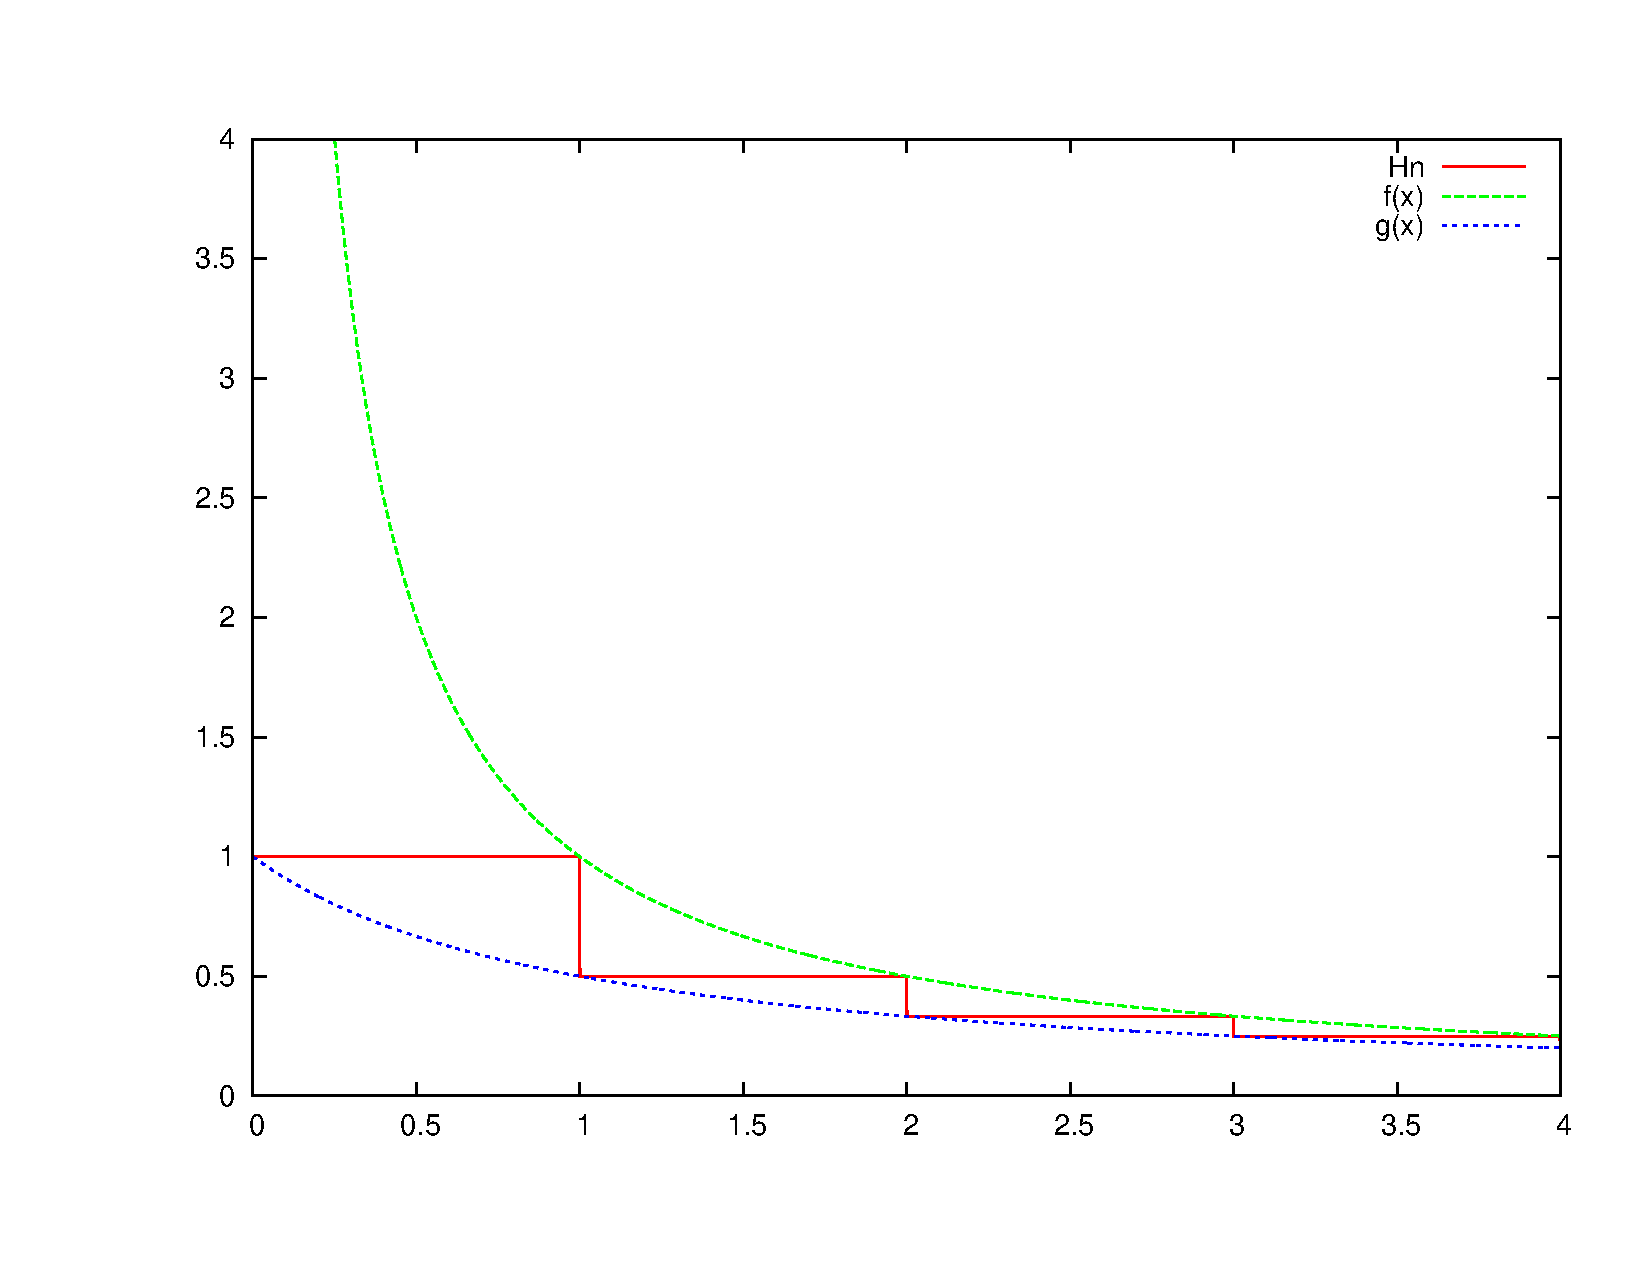
\includegraphics[width=.85\textwidth]{kap1harmonische}
  \caption{$H_n$ zeigt den Teil auf, der bei jedem Schritt der Harmonischen Reihe summiert wird. Die Harmonische Reihe kann geometrisch als die Größe der Fläche von $H_n$ interpretiert werden. $f(x)=\frac{1}{x}$ und $g(x)=\frac{1}{1+x}$ bilden eine obere und untere Schranke.}
  \label{harmonische}
\end{figure}

Die Harmonische Zahl $H_n$ kann geometrisch interpretiert werden, als die Größe der Fläche der Funktion $H_n(x) = \frac{1}{\lceil x \rceil}$, die in Abbildung \ref{harmonische} dargestellt ist. Als obere Schranken können wir $f(x) = \frac{1}{x}$, als untere $g(x) = \frac{1}{x+1}$ angeben. Also können wird $H_n$ mit Hilfe von Integralen abschätzen. Da wir $f(x) = \frac{1}{x}$ nicht von $0$ an abschätzen können, beginnen wir bei $1$ und addieren 1 für alle $ 0 \le x \le 1$ hinzu.
\begin{align*}
  H_n &\le 1 + \int_{1}^{n} \frac{1}{x} dx = 1 + \ln n - \ln 1 = 1 + \ln n \\
  H_n &\ge 1 + \int_{0}^{n} \frac{1}{x+1} dx = \ln (n+1) 
\end{align*}

Wie genau ist diese Abschätzung? Der Unterschied zwischen der oberen und unteren Schranke entspricht der Euler"=Mascheroni"=Konstante, also $\gamma \approx 0,5772156649$. Es gilt somit:
\[ H_n = \ln n + \mathcal{O}(1) \]

Jetzt haben wir alles zusammen, um die Laufzeit von Quicksort abzuschätzen.
\begin{align*}
  C(n) &\le 2(n+1) H_{n+1} \\
       &\le 2(n+1) (\ln n + \mathcal{O}(1)) \\
%       &\le (2n +2) (\ln n + 1)\\
%       &\le 2n \ln n + 2n + 2 \ln n + 2 \\
%       &\le 2n \ln n + 2(n+\ln n +1)\\
       &\le 2n \ln n + \mathcal{O}(n) \\
       &\le \frac{2n \log_2 n}{\log_2 e} + \mathcal{O}(n) \\
       &\approx 1,386 n \log n + \mathcal{O}(n)
\end{align*}
\end{Lza}

Fassen wir die Ergebnisse kurz zusammen und überlegen wir kurz, was dies für die Praxis bedeutet. Mergesort hat eine Laufzeit von $n \log n$. Quicksort hat eine Laufzeit von $1,386 n \log n + \mathcal{O}(n)$. Quicksort ist also etwa um den Faktor $1,39$ langsamer, als Mergesort.

Quicksort ist dennoch in der Realität meist effizienter als Mergesort. Mergesort muss die Daten in zwei getrennten Arrays vorhalten, Quicksort kann immer im selben Array arbeiten. Dadurch muss Quicksort weniger Daten im Speicher lesen und schreiben. Gerade bei großen Mengen kann das ausschlaggebend sein. Übersteigt der benötigte Speicher den Arbeitsspeicher eines Computers, nutzt dieser als zusätzlichen Speicher die Festplatte, was zu deutlich längeren Zugriffszeiten führt. Für bestimmte Probleme werden extra Algorithmen entwickelt, die mehr wert auf kleineren Speicherplatzverbrauch legen, als auf kurze Laufzeiten. Solche Algorithmen werden vor allem in Gebieten gebraucht, in denen Algorithmen auf großen Datenmengen rechnen, wie zum Beispiel der Meteorologie.

Abbildung \ref{groessenvergleich} veranschaulicht, die Anzahl der Vergleiche von Algorithmen bestimmter Laufzeit. Des Weiteren wird die Größe von Problemen verglichen, die ein Computer lösen kann, der $10^9$ beziehungsweise $10^{10}$ Vergleiche pro Sekunde bewältigen kann.

\begin{figure}[hbt]
  \centering
  \subfloat[Anzahl von Vergleichen für Algorithmen bestimmter Laufzeiten]{
    \begin{tabular}{>{$}r<{$}>{$}r<{$}>{$}r<{$}>{$}r<{$}}
      n & n \log n & \frac{1}{2} n^2 - \frac{1}{2} n & n! \\\hline\hline
      10 & 33 & 45 & 3{,}6 \cdot 10^{6} \\
      20 & 86 & 190 & 2{,}4 \cdot 10^{18} \\
      50 & 282 & 1225 & 3{,}0 \cdot 10^{64}\\\hline\hline
    \end{tabular}
  }
  
  \subfloat[Größe von Problemen, die eine Maschine lösen kann, welche $10^9$ Vergleiche in der Sekunde verarbeitet]{
    \begin{tabular}{l>{$}r<{$}>{$}r<{$}>{$}r<{$}}
                  & n \log n        & \frac{1}{2} n^2 - \frac{1}{2} n & n! \\\hline\hline 
      $1$ Sekunde & 4 \cdot 10^7    & 4 \cdot 10^4 & 13 \\
      $1$ Stunde  & 1 \cdot 10^{11} & 2{,}6 \cdot 10^6 & 16\\\hline\hline
    \end{tabular}
  }
  \quad
  \subfloat[Größe von lösbaren Problemen auf einer zehnmal schnelleren Maschine]{
    \begin{tabular}{l>{$}r<{$}>{$}r<{$}>{$}r<{$}}
                  & n \log n            & \frac{1}{2} n^2 - \frac{1}{2} n & n! \\\hline\hline 
      $1$ Sekunde & 3{,}5 \cdot 10^8    & 1 \cdot 10^5                    & 14 \\
      $1$ Stunde  & 9{,}1 \cdot 10^{11} & 8{,}4 \cdot 10^6                & 17 \\\hline\hline
    \end{tabular}
  }
  \caption{Übersicht über die Vergleiche bei Algorithmen bestimmter Laufzeitklasse und ihre lösbarkeit auf Maschinen verschiedener Größe.}
  \label{groessenvergleich}
\end{figure}

Man sieht in Abbildung \ref{groessenvergleich}, dass die Größe der Probleme nicht proportional mit der Geschwindigkeit des Computers wächst. Ein Computer kann alle Permutationen einer Folge untersuchen, die gerade mal ein Element mehr enthält, als es ein Computer kann, der zehnmal langsamer ist.

\section{Berechnungsmodelle (models of computing)}
Wenn wir Laufzeiten betrachten, sprechen wir bislang über Vergleiche. Wir sollten jedoch versuchen Begriffe wie Algorithmus, Speicherverbrauch und Laufzeit mathematische zu erfassen. Dazu dienen uns Berechnungsmodelle. Berechnungsmodelle sind mathematische Modelle für Rechner, also für Maschinen zum automatisierten Lösen von Problemen.

Wir wollen zwei Berechnungsmodelle betrachten. Zum einen die von Alan Turing erfundene Turingmaschine (TM), zum anderen die Registermaschine (RAM~-- random access machine). Die Definition einer Turingmaschine setzen wir als bekannt voraus.

\begin{Def}[Registermaschine (RAM~-- random access machine)]
\hspace{\parindent}
Eine Registermaschine hat einen Speicher bestehend aus einer unendlichen Anzahl an Zellen $R_0, R_1, \ldots$ Jede Zelle kann eine Zahl $\in \mathbb{Z}$ beliebiger Größe speichern.

Ein Programm ist eine endliche Folge von Befehlen. Befehle können mit einer Registeradresse $R_i$, dem Inhalt eines Registers $(R_i)$ oder einer Konstante $k \in \mathbb{N}$ arbeiten. Ein Befehlssatz könnte zum Beispiel die in Abbildung \ref{rambefehle} dargestellten Befehle umfassen.
\begin{figure}[hbt]
  \centering
  \begin{tabular}{>{\ttfamily}l@{\qquad}p{20em}}
    A := B &  wobei \texttt{A} eine Registeradresse sein muss und \texttt{B} eine Registeradressen der Form $R_i$, der Inhalt eines Registers der Form $(R_i)$ oder eine Konstanten $\in \mathbb{N}$ sein kann\\
    A := B op C & für arithmetische Operatoren, wie die Addition, Subtraktion, Multiplikation und ganzzahlige Division \\
    GOTO L & wobei \texttt{L} eine Zeile des Programms ist \\
    GGZ B, L & zur Zeile \texttt{L} des Programms springt, wenn $B > 0$ \\
    GLZ B, L & zur Zeile \texttt{L} des Programms springt, wenn $B < 0$ \\
    GZ B, L & zur Zeile \texttt{L} des Programms springt, wenn $B = 0$ \\
    HALT & Die Abarbeitung des Programms beendet.
  \end{tabular}
  \caption{Möglicher Befehlssatz einer Registermaschine}
  \label{rambefehle}
\end{figure}
\end{Def}

Die Semantik eines Befehls kann man auch formaler fassen. Den Zustand einer Registermaschine kann man durch eine Funktion $c : \mathbb{N} \to \mathbb{Z}$ beschreiben, die zu jeder Speicherzelle $R_i$ den dort gespeicherten Wert angibt. Die Semantik eines Befehls kann man dann als Abbildung eines Zustandes auf einen anderen definieren, die vollständige operationelle Semantik lässt sich also beschreiben, in dem man für alle Befehle und Zustände ihre Folgezustände angibt.

\begin{Def}[Registermaschine berechnet Funktion]
\hspace{\parindent}Die Berechnung einer Funktion durch eine Registermaschine kann man definieren als: $f : \mathbb{Z}^* \to \mathbb{Z}^*$, wobei $\mathbb{Z}^*$ die Menge aller endlichen Folgen ganzer Zahlen ist. Das bedeutet falls die Folge $a_0, a_1, \ldots, a_k$ in den Zellen $0, 1, \ldots, k$ steht, dann wird das Programm bis zum \texttt{HALT}-Befehl ausgeführt. Danach steht in den ersten $s$ Zellen $b_0, b_1, \ldots, b_s$. Das heißt, die Berechnung einer Funktion durch eine Registermaschine ist eine Funktion, die Zustände auf Zustände abbildet, wobei es eine Folge von Befehlen geben muss, die den Startzustand gegebenenfalls über Zwischenzustände in den Endzustand überführen.
\end{Def}

\subsection{Laufzeit und Speicherbedarf (Komplexitätsmaße)}
Laufzeit und Speicherbedarf eines Algorithmus dienen als Maß seiner Komplexität.

Bei Turingmaschinen sind Laufzeit und Speicherbedarf klar definiert: Ein Zeitschritt, entspricht der einmaligen Anwendung der Überführungsfunktion und damit einem Schritt des Kopfes auf dem Band der TM. Der Speicherplatz gleicht der Anzahl der benutzten Zellen auf dem Band. Formal ausgedrückt: Die Laufzeit einer TM ist definiert als $t(w) = $ Anzahl der Schritte, bis TM hält. Der Speicherbedarf einer TM ist definiert als $s(w) = $ Anzahl der benutzten Zellen des Bandes bei Eingabe $w$, bis TM hält.

Bei Registermaschinen gibt es zwei Sichtweisen, das logarithmische Kostenmaß (LKM) und das Einheitskostenmaß (EKM).

\begin{Def}[Einheitskostenmaß (EKM)]\label{defEKM}
\hspace{\parindent}Im Einheitskostenmaß kostet das Ausführen eines Befehls immer eine Zeiteinheit, unabhängig von der Komplexität des Befehls oder seinen Operanden. Für den Speicherbedarf im Einheitskostenmaß entspricht jedes Register einer Speichereinheit, unabhängig von der Größe seines Inhalts. Die Laufzeit einer Registermaschine im EKM ist also definiert als $t(x) = $ Anzahl ausgeführter Befehle bis zum ersten Erreichen des \texttt{HALT}-Befehls. Der Speicherplatzbedarf einer Registermaschine im EKM ist also definiert als $s(x) =$ in einem Schritt maximal benutzte Anzahl von Registern über alle Befehle.
\end{Def}

In der Realität wir eine Addition von zwei 1000-stelligen Zahlen mehr Laufzeit und Speicherplatz brauchen, als die Addition von zwei dreistelligen Zahlen.

\begin{Def}[Logarithmisches Kostenmaß (LKM)]\label{defLKM}
\hspace{\parindent}Das logarithmische Kostenmaß berücksichtigt die Länge der einzelnen Operanden. Die Laufzeit eines Befehls wird als die Summe der Länge der Binärdarstellung aller Werte des Befehls definiert. Ist $L(n)$ die Länge eines Operanden in Binärdarstellung, so ist die Laufzeit eines Befehls als $\sum_{i=1}^{j}L(i)$ definiert, wobei der Befehl aus den Werten $1 \ldots j$ besteht. Die Laufzeit eines Algorithmus wird wie im EKM definiert, als $t(x)=$ Summe der Laufzeiten aller ausgeführten Befehle.

Der Speicherplatzbedarf eines Zustandes im logarithmischen Kostenmaß wird als die Summe der Länge aller in Registern gespeicherter Werte in Binärdarstellung zuzüglich ihrer Adressen in Binärdarstellung definiert. Der Speicherplatzbedarf einer Registermaschine ist wieder definiert, als der in einem Schritt maximal benutzte Speicherplatz über alle Befehle. Anders ausgedrückt wird der Speicherplatzbedarf einer Registermaschine im logarithmischen Kostenmaß definiert, als der Speicherplatzbedarf des Zustands, der vom Start der Berechnung bis zum Erreichen das \texttt{HALT}-Befehls den meisten Speicherplatz verbraucht hat.
\end{Def}

\subsection{Komplexität}
Komplexität ist der Überbegriff für die unterschiedlichen Komplexitätsmaße, wie Laufzeit und Speicher. Wir unterscheiden dabei drei Fälle: die Komplexität im schlechtesten, im mittleren Fall und die erwartete Komplexität bei Zufallsalgorithmen.

Zur Berechnung des schlechtesten Falls betrachten wir das untersuchte Komplexitätsverhalten über alle Eingaben der Länge $n$ und nehmen davon das Maximum:
\begin{align*}
  T(n) &= \max_{|x|=n} t(n) \\
  S(n) &= \max_{|x|=n} s(n)
\end{align*}

Im Mittel gilt, dass $T(n)$ der Erwartungswert von $t(x)$ ist, wobei $x$ eine Eingabe der Länge $n$ ist. Zum Berechnen des Erwartungswertes brauchen wir die Wahrscheinlichkeitsverteilung auf der Menge der Länge der Eingaben. Bei der Analyse des deterministischen Quicksort-Algorithmus gehen wir davon aus, dass alle Permutationen der Eingabefolge mit gleicher Wahrscheinlichkeit auftreten.

Zufallsalgorithmen werden auch probabilistische oder randomisierte Algorithmen genannt. Sie verwenden den Zufall, um einzelne Entscheidungen zu treffen, zum Beispiel für die Auswahl eines Pivotelements. Hier hilft es nicht über alle Eingaben zu mitteln. Statt dessen muss der Erwartungswert über alle zufälligen Entscheidungen betrachtet werden.

Der deterministische Quicksort-Algorithmus hat eine gute Laufzeit im Mittel, es gibt jedoch "`schlechte"' Eingaben, die eine schlechte Laufzeit provozieren. Der randomisierte Quicksort-Algorithmus hat ein gutes Laufzeitverhalten für alle Eingaben.

%Berechnungsmodelle: gewisse mathematische Strukturen, die man Einführt um Algorithmus, Laufzeit u.ä. Begriffe zu modellieren.
%
%Das einfachste Modell ist die Turingmaschine. Laufzeit für TM: die Anzahl der Schritte, Anzahl der angewandeten Überführungsfunktionen, Speicherplatz: benutzte Zellen auf dem Band. Üblicherweise nimmt man das maximum über alle Angaben der Länge n. Man kann auch den Erwartungswert nehmen, dann spricht man von Mittel.
%
%Als weiteres Modell wurde die Registermaschine besprochen (abgekürzt RAM). Zwei Sichweisen: das Einheitskostenmaß (EKM). Egal wie groß die Operanden sind zählt man bei der Ausführung immer eine Zeiteinheit. Daher nicht ganz fair. Das logarithmischen Kostenmaß (LKM) zählt die länge der Binärdarstellungen aller beteiligten Operanden.
%\clearpage

\subsection{Vergleich dieser Berechnungsmodelle}
\begin{Satz}[Zur Laufzeit von RAM und TM]
\hspace{\parindent}Zu einer Registermaschine mit Laufzeit $T(n)$ im logarithmischen Kostenmaß gibt es eine äquivalente Einband-Turingmaschine der Laufzeit $\mathcal{O}(T(n))^5$
\end{Satz}

\begin{Satz}[Zum Speicherplatz von RAM und TM]
\hspace{\parindent}Zu einer Registermaschine mit Speicherplatz S(n) im logarithmischen Kostenmaß gibt es eine äquivalente Einband-Turingmaschine mit Speicherplatzbedarf $\mathcal{O}(S(n))$.
\end{Satz}

Insbesondere gilt, dass alle Probleme, die in polynomieller Zeit oder Platz auf einer Registermaschine mit logarithmischen Kostenmaß lösbar sind, auch in polynomieller Zeit auf einer Turingmaschine lösbar sind. Polynomiell bedeutet, dass die Laufzeit in $\mathcal{O}(n^k)$ liegt, für ein $k \in \mathbb{N}$.

\begin{Bem}[Komplexitätsklasse \textsf{P}]
\hspace{\parindent}Diese Klasse von Problemen, die in polynomieller Laufzeit lösbar sind, heißt \textsf{P}. Die Klase von Problemen, die in polynomiellem Speicherplatz lösbar sind, heißt \textsf{PSPACE}.
\end{Bem}

\section{Darstellung von Algorithmen und ihre Laufzeitanalyse}
\subsection{Pseudocode}
Algorithmen werden meist nicht als Register- oder Turingmaschinen dargestellt, stattdessen werden Konstrukte höherer Programmiersprachen genutzt, wie z.B. \texttt{if}, \texttt{for}, \texttt{while} oder Rekursion, zum Teil sogar vermischt mit umgangssprachlichen Anweisungen. Diese Art der Darstellung nennt man \textit{Pseudocode}.

Die Umsetzung in Code einer Registermaschinen sollte offensichtlich sein. Die Analyse von Algorithmen ist auch möglich, wenn sie in Pseudocode vorliegen, zumindest in Form von $\mathcal{O}$ oder $\Theta$.

\subsection{Beispiel Sortieralgorithmen}
Betrachten wir zum Beispiel die Sortieralgorithmen \ref{Bogosort} bis \ref{Alter-Mann}. Ihre Laufzeit\footnote{So nicht anders angegeben betrachten wir Laufzeit, Speicherplatz usw. immer im Einheitskostenmaß. Betrachten wir solche Werte nach dem logarithmischen Kostenmaß, weißen wir speziell darauf hin.} auf einer Registermaschine ist proportional zur Anzahl der Vergleiche. Das ist keine triviale Aussage, sondern eine Aussage, die unter Betrachtung der Algorithmen im Pseudocode gewonnen werden kann. Damit ist zum Beispiel die Laufzeit von Mergesort $\Theta(n \log{n})$ auf einer Registermaschine.

\begin{center}
\begin{tabular}{lcc}
 & Anz. Vergl. & RAM (EKM) \\\hline\hline
Minimum Auswahl & $ \frac{1}{2} n^2 $ & $2{,}5 n^2$ \\
Mergesort & \textasciitilde $n \log{n}$ & $12 n \log{n}$ \\
Randomisiertes Quicksort & \textasciitilde  $1{,}38 n\log{n}$ & $9 n \log{n}$ \\\hline\hline
\end{tabular}
\end{center}

\subsection{Rekursion}
Rekursion wird zum Beispiel von der Algorithmen-Entwurfsstrategie divide~\& conquer (Teile und herrsche) genutzt. Um ein Problem der Größe $n$ zu lösen, wird es in kleinere Teilprobleme zerlegt. Diese löst man rekursiv und kombiniert ihre Lösungen zu einer Lösung des Gesamtproblems.

Liefert die Laufzeitanalyse eines Algorithmus eine Rekursionsgleichung, so muss diese aufgelöst werden (vergleiche z.B. die Laufzeitanalyse \ref{QuicksortLza} von Quicksort auf S. \pageref{QuicksortLza}). Die Nutzung von Rekursion in Algorithmen beinhaltet die Gefahr exponentielle Laufzeit zu bekommen (siehe Übung).

Neben der Laufzeit spielt auch der Platzbedarf gerade bei rekursiven Algorithmen eine große Rolle. Während der Laufzeit wird ein Stack aufgebaut, der für alle rekursiven Aufrufe einen activation record, einen Datensatz mit allen Laufzeitinformationen, enthält. Unter der Annahme, dass die Datensätze im Laufzeitstack konstante Größe haben, ist der Speicherplatzbedarf für diesen Stack ist so hoch, wie die Tiefe der Rekursion sein kann.

\begin{Bsp}[Fakultät]
\hspace{\parindent}
Die Fakultät lässt sich rekursiv berechnen:
\begin{align*}
fak(0) &= 1 \\
fak(n) &= fak(n-1) \cdot n
\end{align*}

Dieses Vorgehen hat einen Speicherplatzbedarf von $\Theta (n)$. Die Fakultät lässt sich aber auch durch eine einfache Schleife berechnen, ganz ohne Rekursion und ohne Laufzeitstack.
\end{Bsp}

\subsection{Typische Funktionen}

Betrachten wir einige bei der Analyse von Algorithmen typischerweise auftretende Funktionen, sortiert nach ihrem Wachstum:
\begin{center}
\begin{tabular}{cll}
$\log{\log{n}}$ & \multirow{2}*{$\left.\vphantom{\begin{array}{l}\\\end{array}}\right\rbrace$logarithmisch}\\
$\log{n}$\\
$\sqrt{n}$\\
$n$ & linear & \multirow{4}*{$\left.\vphantom{\begin{array}{l}\\ \\ \\ \end{array}}\right\rbrace$polynomiell}\\
$n \log{n}$\\
$n^2$ & quadratisch\\
$n^3$\\
$\vdots$\\
	$2^n$ & \multirow{3}*{$\left.\vphantom{\begin{array}{l}\\\\\end{array}}\right\rbrace$exponentiell}\\
$n!$\\
$2^{n^2}$\\
$2^{2^n}$ & doppelt exponentiell\\
\end{tabular}
\end{center}

Da $\lim\limits_{n \rightarrow \infty}{\frac{\log{n}}{n^\alpha}} = 0$ wissen wir, dass $\log{n} = o(n^{\alpha})$. $\log{n}$ wächst also schwächer als jedes $n^\alpha, \alpha > 0$, daher auch als $\sqrt{n} = n^{\frac{1}{2}}$.


\chapter{Sortieren und Suchen}
\section{Vergleichsbaummodell}
Das Vergleichsbaummodell modelliert Algorithmen, die nur auf Vergleichen zwischen Elementen der Eingabefolge beruhen. $\mathcal{U}$ sei ein Universum auf dem eine lineare Ordnung $\le$ definiert ist. Die Eingabefolge ist definiert als $a_1, \ldots, a_n \in \mathcal{U}$.

\begin{figure}[htb]
  \centering
  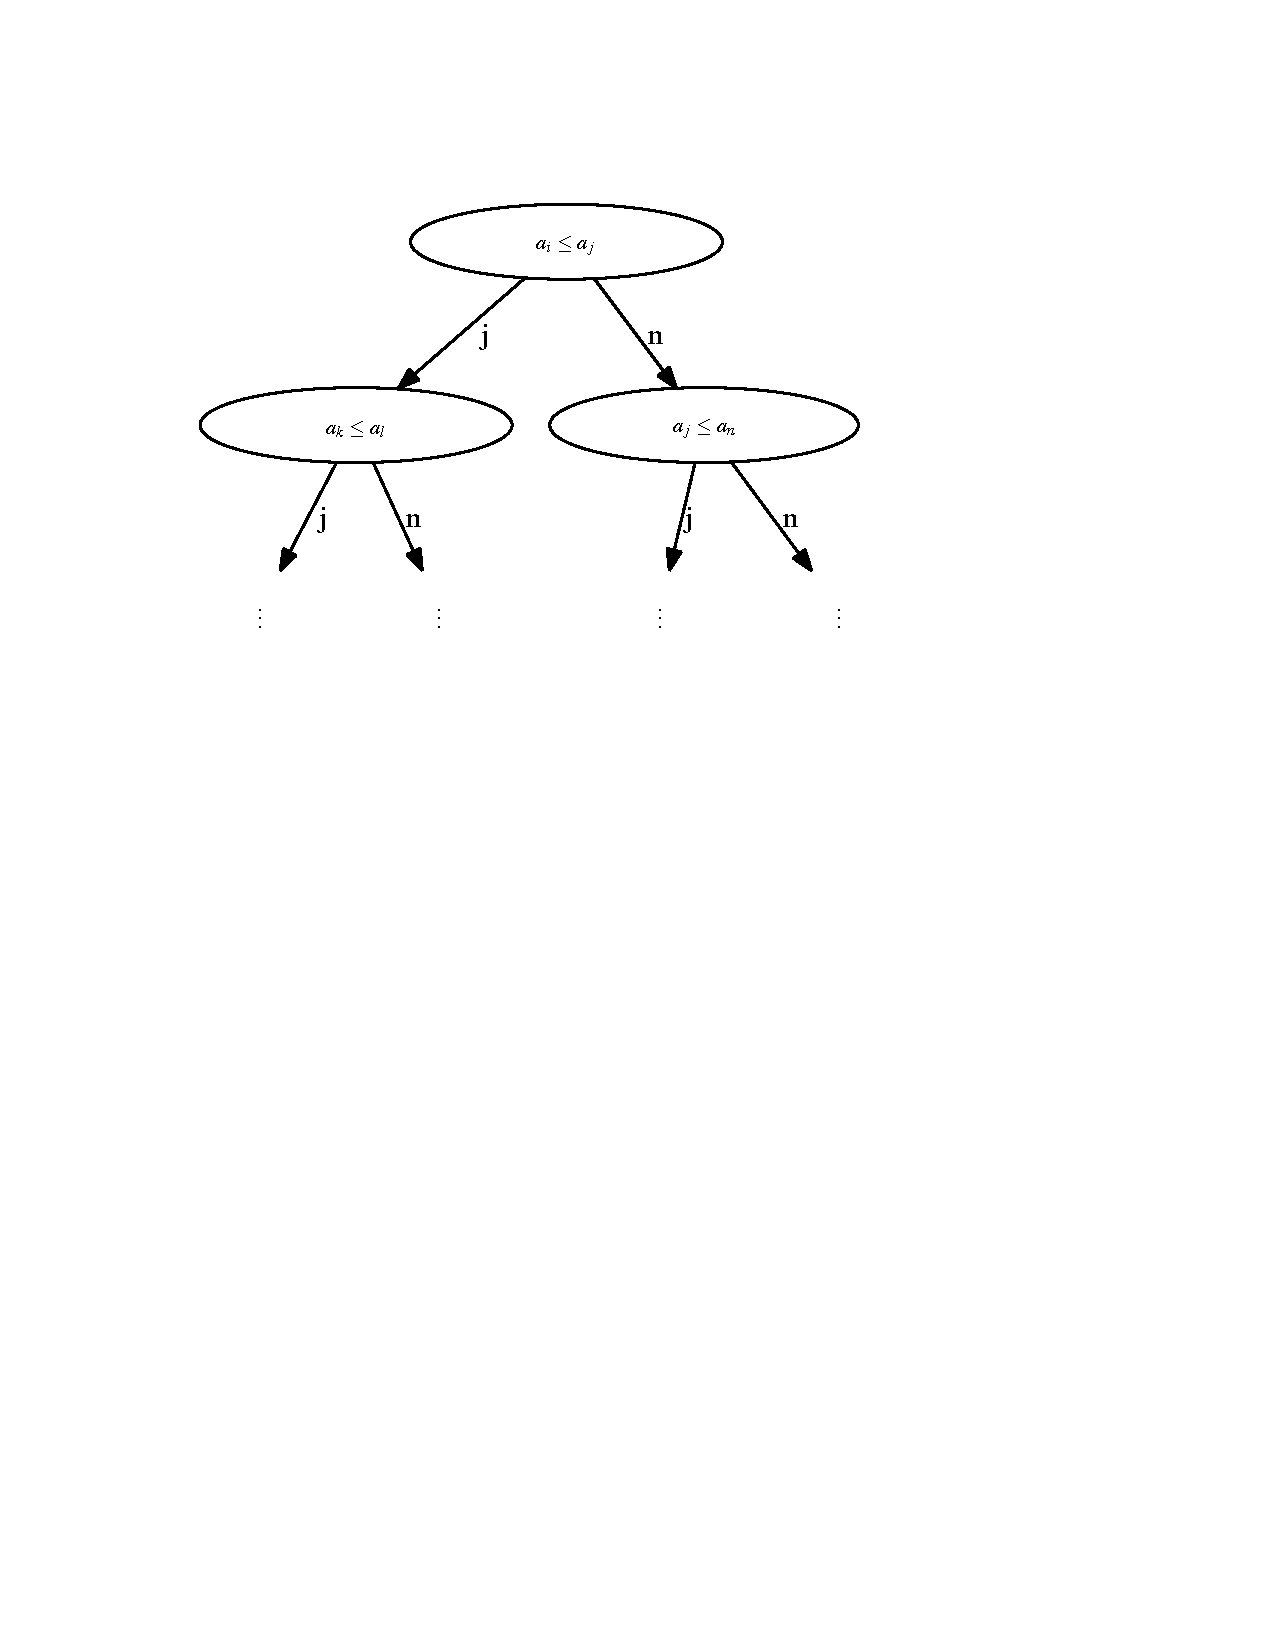
\includegraphics[scale=.75]{kap2graph1.pdf}
  \caption{Vergleichsbaum für einen Algorithmus und eine Eingabe $a_1, \ldots, a_n$}
\end{figure}

Die Algorithmen \ref{Bogosort} bis \ref{Alter-Mann} lassen sich für feste $n$ als Vergleichsbäume darstellen.

\begin{figure}[htb]
  \centering
  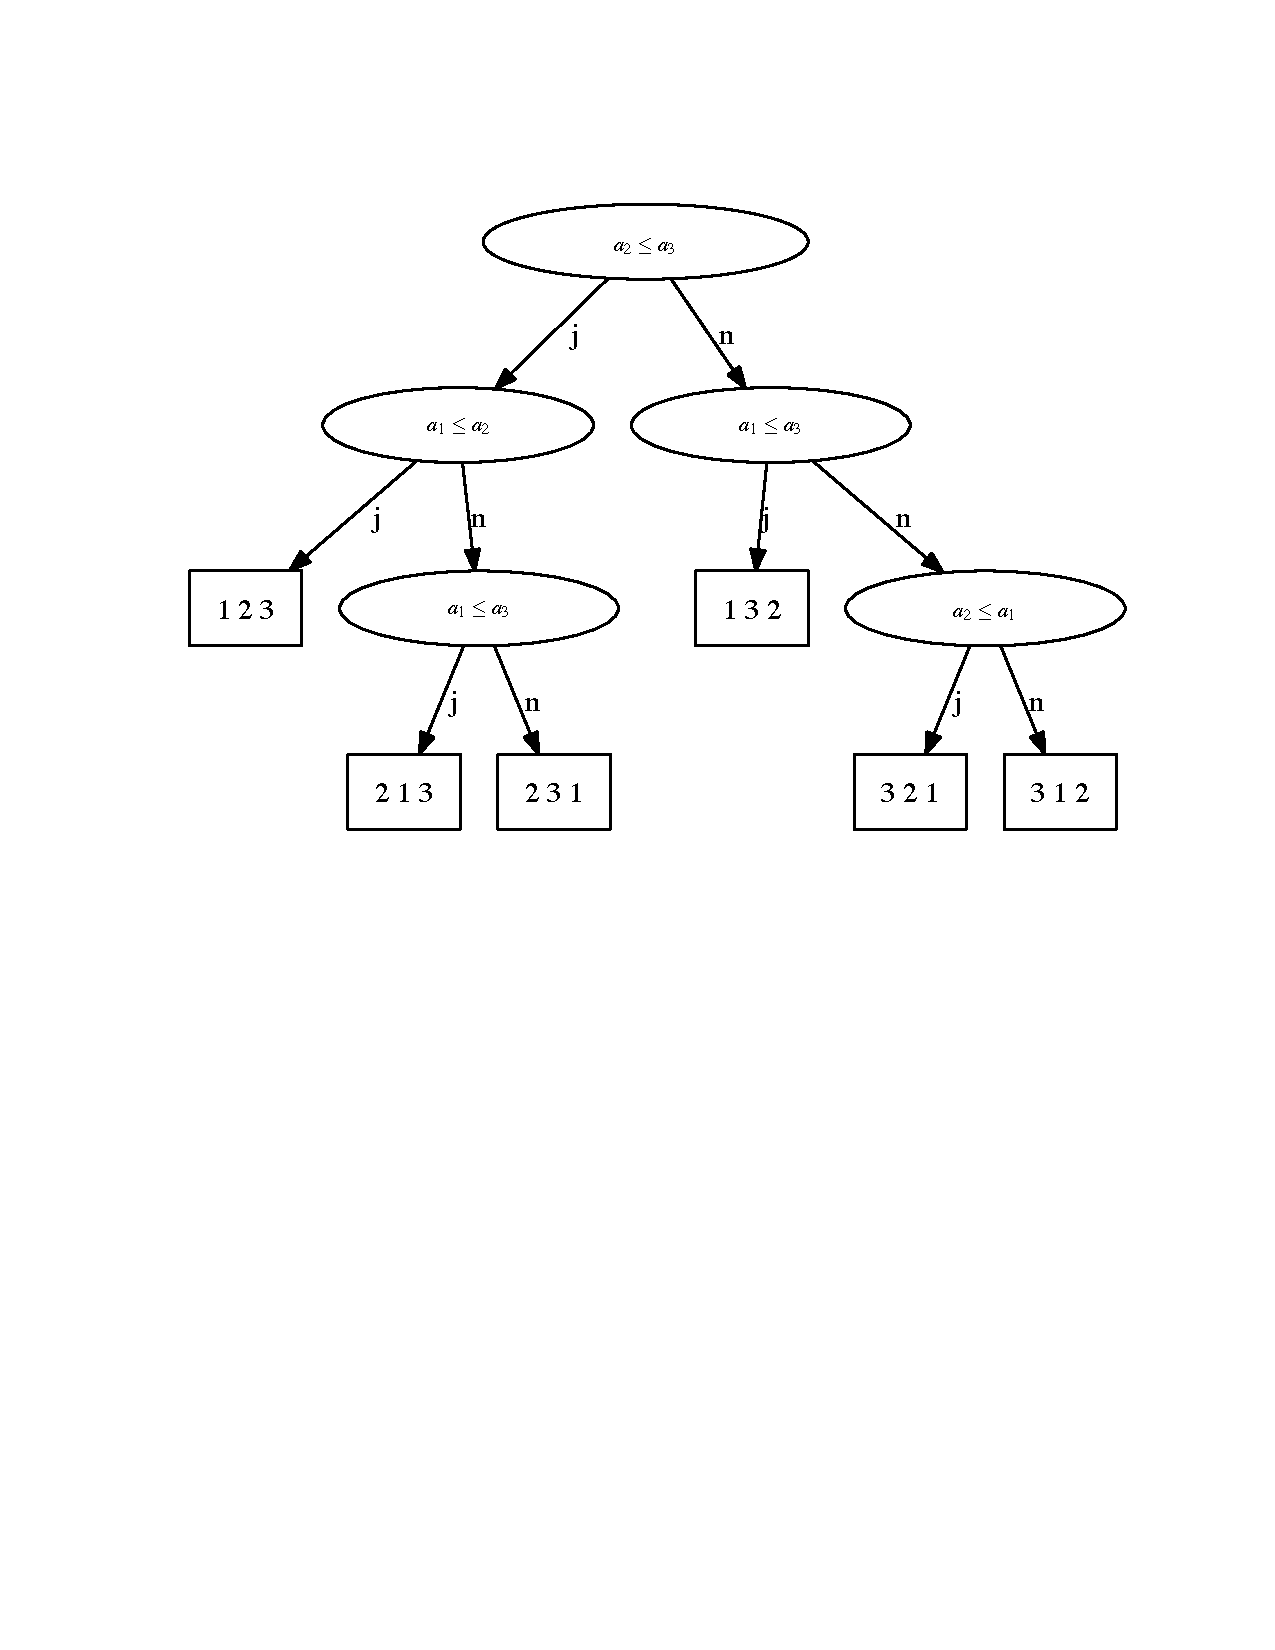
\includegraphics[scale=.75]{kap2graph2.pdf}
  \caption{Vergleichsbaum für Mergesort und die Eingabe $a_1, a_2, a_3$}
\end{figure}

In den Blättern des Vergleichbaums finden wir das Ergebnis des Algorithmus. Für vergleichsbasiertes Sortieren könnnen wir durch den Vergleichsbaum eine untere Schranke zeigen.

\subsection{Untere Schranke für vergleichsbasierte Sortieren}
Allgemeine Sortierverfahren funktionieren auf beliebigen, linear geordnetem Universum. Für allgemeine Sortierverfahren kann man eine untere Schranke zeigen. Für spezielle Universen (z.B. $\lbrace 0, 1 \rbrace$) lassen sich schnellere Sortierverfahren finden.

Eine untere Schranke ist eine Aussage der Form: für jede Eingabe der Länge $n$ braucht man mindestens $T(n)$ Vergleiche. Eine untere Schranke kann auch eine Aussage der Form sein: es gibt eine Eingabe der Länge $n$ zu deren Sortierung man mindestens $T(n)$ Vergleiche braucht. Anstatt auf Vergleichen können sich die Aussagen natürlich auch auch auf Laufzeit, Speicher oder der Gleichen beziehen.

Ein Vergleichsbaum zum Sortieren einer Folge der Länge $n$ muss mindestens $n!$ Blätter haben, da $n!$ der Anzahl aller möglichen Permutation einer Folge der Länge $n$ entspricht. Ein Vergleichsbaum ist binär, das heißt bei Höhe $h$ hat er maximal $2^h$ Blätter. Die Höhe entspricht einem Lauf durch den Vergleichsbaum von oben nach unten mit einer maximal langen Folge von Vergleichen. Die Anzahl der Blätter lässt sich also durch $2^h \ge \text{Anzahl der Blätter} \ge n!$ abschätzen, mit $h \ge \log n!$.
Wir können $n!$ wie folgt abschätzen:
\[n! = 1 \cdot 2 \cdot \ldots \cdot \frac{n}{2} \cdot \underbrace{\left(\frac{n}{2}+1\right) \cdot \ldots \cdot n}_{\ge \frac{n}{2}} \ge \frac{n}{2}^{\frac{n}{2}}\]
Also gilt $\log n^n \ge \log n! \ge \log \frac{n}{2}^{\frac{n}{2}}$. Genauer lässt sich $n!$ noch durch die Stirlingsche Formel abschätzen: $n! = \sqrt{2 \pi n} \left(\frac{n}{e}\right)^n e^{\frac{\Theta}{12n}}$ wobei $0<\Theta<1$.

Wegen der Logarithmengesetze  ist $\log \frac{n}{2}^{\frac{n}{2}} = \frac{n}{2} (\log n-1)$. Mit den Logarithmengesetzen und der Stirlingschen Formel können wir $\log n!$ wie folgt abschätzen.

\begin{align*}
\log n! &= \log \left(\sqrt{2 \pi n} \left(\frac{n}{e}\right)^n e^{\frac{\Theta}{12n}}\right) \\
          &= \frac{1}{2} \log n + \frac{1}{2} \log 2 \pi + n (\log n - \log e) + \frac{\Theta}{12n} \log e\\
%          &= \frac{1}{2} \log n + n\left(\log n - \log e \right) + \log e \frac{\Theta}{12n} + \frac{1}{2}\log 2 \pi \\
          &= n \log n - n \log e + \frac{1}{2} \log n + \frac{1}{2} \log 2 \pi +  o(1)
\end{align*}

$\lim\limits_{n \rightarrow \infty}{o(1)} = 0$, also ist $h \ge n \log{n} - \mathcal{O}(n)$ für hinreichend große $n$.

\begin{Satz}[Untere Schranke für vergleichsbasiertes Sortieren]
\hspace{\parindent}Im Vergleichsbaummodell braucht jeder Algorithmus zum Sortieren einer Folge der Länge $n$ im schlechtesten Fall mindestens $n \log{n} -\mathcal{O}(n)$ Vergleiche.
\end{Satz}

Das heißt man kann nicht schneller sortieren als $n \log{n} -\mathcal{O}(n)$. Für spezielle Universen kann man das wie gesagt schlagen, im Allgemeinen Fall aber nicht.

%\section{Berechnungsbaummodell}
Algebraische Berechnungsbäume sind ein erweitertes Modell der Vergleichsbäume. Vergleichsbäume werden dabei um Rechnungen erweitert, so dass in algebraischen Berechnungsbäumen auch $+, -, *, /$ verwendet werden können.

Auch mit diesem Modell lässt sich $\Omega(n \log n)$ als untere Schranke für allgemeine Sortierverfahren zeigen.

\subsection{Weitere untere Schranken}
\begin{Exk}[Landau-Notation]
\hspace{\parindent}Landau-Symbole werden verwendet, um das asymptotische Verhalten von Funktionen und Folgen zu beschreiben.

\begin{center}
\begin{tabular}{lp{14em}c}
Notation & Bedeutung & math. Definition \\\hline\hline
$f \in \mathcal{O}(g)$ & obere Schranke: $f$ wächst nicht wesentlich schneller als $g$ & $0 \le \limsup\limits_{x \to a} \left|\frac{f(x)}{g(x)}\right| < \infty$ \\
$f \in o(g)$ &$f$ wächst langsamer als $g$ (asymptotisch vernachlässigbar)&$\lim\limits_{x \to a} \left|\frac{f(x)}{g(x)}\right| = 0$\\
$f \in \Omega(g)$ &$f$ wächst nicht wesentlich langsamer als $g$ (untere Schranke)&$0 < \liminf\limits_{x \to a} \left|\frac{f(x)}{g(x)}\right| \le \infty$\\
$f \in \omega(g)$ &$f$ wächst schneller als $g$ ($g \in o(f)$)&$\lim\limits_{x \to a} \left|\frac{f(x)}{g(x)}\right| = \infty$\\
$f \in \Theta(g)$ &$f$ und $g$ wachsen gleich schnell ($f \in \mathcal{O}(g)$ und $g \in \mathcal{O}(f)$)&$0 < \liminf\limits_{x \to a} \left|\frac{f(x)}{g(x)}\right| \le \limsup\limits_{x \to a} \left|\frac{f(x)}{g(x)}\right|< \infty$\\\hline\hline
\end{tabular}
\end{center}
\end{Exk}

$\Omega(n \log n)$ gilt nicht nur für allgemeine Sortiverfahren als untere Schranke. Ein anderes Problem mit der selben unteren Schranke ist das Problem der \textit{Mengengleichheit}. Gegeben sind zwei Mengen über einem Universum: $S, T \subseteq \mathcal{U}$. Gefragt ist, ob $S$ und $T$ gleich sind, also $S=T$? Entscheiden lässt es sich in $n \log n$, in dem man beide Mengen sortiert und anschließend in linearer Zeit vergleicht.

Ein weiteres Problem der Art ist das Problem der \textit{element uniqueness}. Gegeben ist eine Folge $S \subseteq \mathcal{U}$ der Länge $n$ mit den Elementen $a_1, \ldots a_n$. Gibt es $i,j$ mit $i\neq j$, so dass gilt $a_i = a_j$?

Es gibt nicht viele Probleme mit bekannten unteren Schranken. Interessant ist, dass es noch andere Wege gibt die untere Schranke für allgemeine Sortierverfahren zu zeigen, als über das Vergleichsbaummodell.

Wir wollen hier aber noch ein Problem mit einer anderen unteren Schranke betrachten: \textit{Finden des Maximums}. Das triviale Vorgehen ist sicherlich das erste Element mit dem zweiten zu vergleichen und sich das Größere der beiden zu merken. Alle weiteren Elemente werden dann mit dem bis dahin gefundenen Maximum verglichen, so dass man auf eine Laufzeit von $n-1$ kommt. Warum geht es aber nicht schneller als mit $n-1$ Vergleichen? Jedes Element, das nicht als Maximum deklariert wird, muss in einem Vergleich unterlegen gewesen sein: Es gibt im allgemeinen Fall keine Möglichkeit zu erkennen, dass ein Element nicht das Maximum ist, ohne es zu Vergleichen. Jedes Element muss also mind. einmal verglichen worden sein, daher braucht man mindestens $n-1$ Vergleiche.

\section{Sortieren in linearer Zeit}
Sortieren in linearer Zeit lässt sich weder im Vergleichsbaummodell realisieren noch für den allgemeinen Fall. Wir wollen hier Algorithmen betrachten, die spezielle Universen in linearer Zeit sortieren. Betrachten wir zunächst das Universum $\mathcal{U} = \lbrace 0, 1 \rbrace$. Hier kann man in $\mathcal{O}(n)$ mit zwei Zählern sortieren, indem man erst alle $0$- und dann alle $1$-Elemente zählt und anschließend die richtige Anzahl in der richtigen Reihenfolge ausgibt. Verallgemeinert auf beliebige endliche Universen $\mathcal{U} = \lbrace c_1, \ldots, c_k\rbrace$ braucht man $k = |\mathcal{U}|$ Zähler.

\textit{Bucketsort} ist eine Verallgemeinerung des Sortierens in linearer Zeit. Allen zu sortierenden Elemente muss dazu ein Wert zugewiesen werden können. Die Eingabe kann dann als Intervall angesehen werden, dass in gleichgroße Teilintervalle aufgeteilt werden kann, in sogenannte "`Buckets"'. In diese Buckets werden dann die Elemente einsortiert. Wenn die Elemente gleichverteilt sind und die Anzahl der Buckets der Anzahl der Elemente entspricht (ein Element pro Bucket), so arbeitet Bucketsort in linearer Zeit. Andernfalls müssen die Buckets intern sortiert und dann konkateniert ausgegeben werden. Bucketsort hat dann die Laufzeit des Algorithmus, der zum Sortieren der Buckets genutzt wird. Diese Verfahren ist zum Beispiel gut geeignet, um Briefe anhand von Postleitzahlen zu sortieren.

\textit{Radixsort} ist ein Algorithmus zum Sortieren von Wörtern $\in \Sigma^*$ mit $\Sigma$ endliches Alphabet. Es basiert auf Bucketsort. Das Ziel ist es die eingegebenen Wörter in lexikographische Ordnung zu bringen. Dabei hat jeder Buchstabe in einem Wort ein unterschiedliches Gewicht, je nach seiner Position (größtes Gewicht hat der erste Buchstabe, kleinstes Gewicht der letzte). Radixsort sortiert die Wörter wie folgt: zu erst werden die Wörter anhand ihres letzten Buchstaben sortiert. In weiteren Läufen werden die Buchstaben von hinten nach vorne verglichen und die Reihenfolge der Wörter nur verändert, wenn die betrachteten Buchstaben nicht in lexikographischer Ordnung stehen. Ein Beispiel ist in Abb. \ref{radixBsp} zu sehen.

\begin{figure}[hbt]
\centering
\begin{tabular}{ccccccc}
Mon & \multirow{4}{*}{$\xrightarrow{\stackrel{\text{\small letzer}}{\text{\small Buchstabe}}}$} & Die & \multirow{4}{*}{$\xrightarrow{\stackrel{\text{\small vorletzer}}{\text{\small Buchstabe}}}$}& Die & \multirow{4}{*}{$\xrightarrow{\stackrel{\text{\small erster}}{\text{\small Buchstabe}}}$} & Die \\
Die &  & Mon & & Mit & & Don \\
Mit &  & Don & & Mon & & Mit \\
Don &  & Mit & & Don & & Mon \\
\end{tabular}
\caption{Radixsort auf den Wörtern Mon, Die, Mit, Don.}\label{radixBsp}
\end{figure}


Radixsort braucht $\mathcal{O}(n)$ Zeit, wobei $n$ der Gesamtzahl der Buchstaben aller Wörter entspricht.

\section{Das Auswahlproblem (selection, order statistics, Select)}
Betrachten wir das Auswahlproblem: Als Eingabe bekommen wir eine Folge $S$ von $n$ Elementen aus dem Universum $(\mathcal{U}, \le)$ und die Zahl $k$ mit $1 \le k \le n$. Gesucht ist das k-t-kleinste Element von $S$, also das Elemente, das an Stelle $k$ der Folge $S$ steht, wenn sie aufsteigend sortiert ist. Dieser Ansatz --~sortieren der Folge und abzählen der Stelle $k$~-- liefert bereit einen Algorithmus, mit Laufzeit $\mathcal{O}(n \log n)$. Geht das noch schneller?

\subsection{Randomisiertes Select}
\begin{Alg}[SELECT(k, S)]
	\begin{enumerate}
	  \item Falls $|S|=1$ (also $S = \lbrace a \rbrace$), return $a$, sonst:
	  \item Wähle zufällig ein Element $a \in S$.
	  \item Spalte $S$ in drei Teilfolgen: $S_1 = \lbrace\text{Elemente} < a\rbrace$, $S_2 = \lbrace\text{Elemente} = a\rbrace$ und $S_3 = \lbrace\text{Elemente} > a\rbrace$.
	  \item Falls $k \leq |S_1|$, dann return \textsc{Select}$(k, S_1)$.
	  \item Falls $k \leq |S_1| + |S_2|$ dann return $a$.
	  \item Sonst return \textsc{Select}$(k-|S_1| - |S_2|, S_3)$.
	\end{enumerate}
\end{Alg}

Dieser Algorithmus ist mit Quicksort vergleichbar. Er hat die gleiche Schwäche: Wenn man $a$ ungünstig wählt, ist die Laufzeit im schlechtesten Fall $\Theta(n^2)$. Doch wie ist die erwartete Laufzeit, also die Laufzeit im Mittel?

Der Rekursionsanker ist einfach zu finden: $T(1) = b$, wobei $b$ konstant ist. Stellen wir die Rekursionsgleichung für $T(n)$ auf: Sei $a$ das $i$-t-kleinste Element (also das Element an Stelle $i$, falls die Folge aufsteigend sortiert ist). Dann ist $S_1 = \{ a_1, \ldots, a_{i-1}\}$, $S_2 = \{ a_i \}$ und $S_3 = \{ a_{i+1}, \ldots , a_n \}$ . Jedes $i \in \{1, \ldots, n\}$ hat eine Wahrscheinlichkeit von $\frac{1}{n}$. Falls $i<k$, so liegt das gesuchte Element in $S_3$. Wir starten also eine rekursive Suche in $S_3$, einer Teilfolge der Größe $n-i$. Angenommen $i > k$, so liegt das gesuchte Element in $S_1$, also in einer Teilfolge der Größe $i-1$. Der Fall $i=k$ ist durch $T(1)$ bereits abgedeckt. Die Rekursionsgleichung lässt sich daher wie folgt aufstellen:

\[ T(n) = \frac{1}{n} \left(\vphantom{\sum_{i=1}^{k-1}}\right. \underbrace{\sum_{i=1}^{k-1} T(n-i)}_{\text{rek. Aufruf für} S_3} + \underbrace{\sum_{i=k+1}^{n} T(i-1)}_{\text{rek. Aufruf für} S_1} \left.\vphantom{\sum_{i=1}^{k-1}}\right) + \underbrace{c \cdot n}_{\text{fürs Aufteilen}}\]

Betrachten wir kurz die beiden Summen in dieser Gleichung. In der ersten Summe verläuft $i$ von $1$ bis $k-1$. Es wird also summiert über $T(n-1) + T(n-2) + \ldots + T(n-k+1)$. In der zweiten Summe verläuft $i$ von $k+1$ bis $n$. Es wird also summiert über $T(k) + \ldots + T(n-2) + T(n-1)$.

\begin{figure}[hbt]
  \centering
  \includegraphics{kap2strahl1}
  \caption{Angenommen $k \leq \frac{n}{2}$. Der mittlere Bereich visualisiert die erste, der untere die zweite Summe. Der blaue gepunktete Bereich entspricht: $k \ldots \frac{n}{2}$, der grüne gestrichelte größere Bereich $\frac{n}{2} \ldots (n-k+1)$.}
  \label{kap2strahl1}
\end{figure}

Angenommen $k \leq \frac{n}{2}$. Wir können $k \ldots \frac{n}{2}$ durch $\frac{n}{2} \ldots n-k+1$ ersetzen, da $T$ monoton steigend und somit der ersetzte Bereich kleiner ist, als der ersetzende Bereich. In Abbildung \ref{kap2strahl1} wird das ganze veranschaulicht: wir ersetzen den blauen, durch den grünen Bereich. Dadurch können wir die beiden Summen zu einer zusammenfassen, und schreiben:
\[T(n) \leq \frac{2}{n} \sum_{i= \lfloor \frac{n}{2} \rfloor}^{n-1} T(i) + c \cdot n\]

Behauptung: $T(n) = \mathcal{O}(n)$. Das heißt $\exists{} d > 0 : T(n) \le d n$ für alle $n \in \mathbb{N}$. Wir wollen das durch Induktion über n beweisen.

Wir nehmen an, dass eine Konstante $d$ existiert, so dass gilt $T(n) \le d \cdot n$.
Als Induktionsanfang dient uns $n=1$. Anhand von Zeile $1$ des Algorithmus kann man sehen, dass $T(1) = b \le d$. Für ein geeignet gewähltes $d \ge b$ ist das richtig.
Es folgt der Induktionsschritt $(n-1) \rightarrow n$:

\[T(n) \le \frac{2}{n} \sum_{i= \lfloor \frac{n}{2} \rfloor}^{n-1} T(i) + cn\]
Aufgrund der Induktionsvoraussetzung können wir annehmen, dass 
\[\sum_{i= \lfloor \frac{n}{2} \rfloor}^{n-1} T(i) \le \sum_{i= \lfloor \frac{n}{2} \rfloor}^{n-1} d \cdot i\]
Daher gilt:
\[T(n) \le \frac{2d}{n} \sum_{i=\lfloor\frac{n}{2}\rfloor}^{n-1} i + cn\]
Die Summe schätzen wir mit dem Satz von Gauß ab, wobei wir aufgrund des Laufindex der Summe den zu viel berechneten Teil subtrahieren müssen.
\[ T(n) \le \frac{2d}{n} \left( \frac{n(n-1)}{2} - \frac{\lfloor \frac{n}{2} \rfloor(\lfloor \frac{n}{2} \rfloor -1)}{2} \right) + cn \qquad \lfloor \frac{n}{2} \rfloor \ge \frac{n}{2}-1 \]
Unter Berücksichtigung der Abschätzung $\lfloor \frac{n}{2} \rfloor \ge \frac{n}{2} -1$ können wir schreiben:
\begin{align*}
T(n) & \le \frac{2d}{n} \left( \frac{1}{2}n^2 - \frac{1}{2} n - \frac{(\frac{n}{2} -1) (\frac{n}{2}-2)}{2}\right) + cn\\
     & \le \frac{2d}{n} \left( \frac{3}{8} n^2 + \frac{1}{4}n -1 \right) + cn
\end{align*}
Die $-1$ können wir weg lassen, für die Ungleichung ist das unerheblich.
\begin{align*}
T(n) & \le \frac{3}{4}dn + \frac{1}{2}d + cn \\
     &  = \left( \frac{3}{4} d + c \right) n + \frac{d}{2}
\end{align*}
Gegen die $\frac{d}{2}$ können wir noch etwas machen: Die $\frac{3}{4}d$ ersetzen wir durch $0{,}8d$ und ziehen dann $0{,}05dn$ vom zweiten Summanden ab.
\[ T(n) \le (0{,}8 d + c) n + \left(\frac{1}{2} - 0{,}05 n\right) \cdot d \]
Für $n \ge 10$ nimmt $\left(\frac{1}{2} - 0{,}05 n\right) \cdot d$ einen Wert $\le 0$ an, das heißt für diese $n$ ergibt sich:
\[T(n) \le (0{,}8 d + c) n\]
Wir können nun wiederum abschätzen $0{,}8 d + c \le d$ und nach $d \le 5c$ auflösen. So erhalten wir schließlich für $n \ge 10$
\[T(n) \le dn\]

Für $n < 10$ braucht Algorithmus konstant viele Schritte: $T(n) \le e$. Wählen wir $d \ge e$ dann gilt $T(n) \le dn$ für alle $n \in \mathbb{N}$. Die Behauptung gilt also mit $d=max (b, 5c, e)$.

\begin{Satz}
\hspace{\parindent}Der Algorithmus \textsc{Select} löst das Auswahlproblem mit mittlerer Laufzeit $\mathcal{O}(n)$ für Folgen der Länge $n$.
\end{Satz}

\subsection{Deterministisches Select}
Können wir einen deterministischen Select-Algorithmus finden, mit garantierter Laufzeit von $\mathcal{O}(n)$? Wir ersetzen die ersten beiden Zeilen im Select"=Algorithmus durch folgende:

\begin{enumerate}
  \item Falls $|S| < 60$, löse das Problem "`brute force"' zum Beispiel durch sortieren und auswählen. Sonst:
  \item \begin{itemize}
    \item Teile $S$ in $\lceil \frac{n}{5} \rceil$ Teilfolgen der Länge 5
    \item bestimmte von allen Teilfolgen die "`Mediane"' (d.h. k-tes Element für $k=\lceil \frac{5}{2} \rceil$)
    \item bestimme von diesen $\lceil \frac{n}{5} \rceil$ Medianen rekursiv den Median und wähle ihn als Element $a$ aus.
  \end{itemize}
\end{enumerate}

Warum ist die Laufzeit garantiert linear? In Abbildung \ref{mediansuche} sieht man, dass durch ein klug gewähltes $a$ ein konstanter Bruchteil an Elementen wegfällt und nicht untersucht werden muss.

\begin{figure}[htb]
  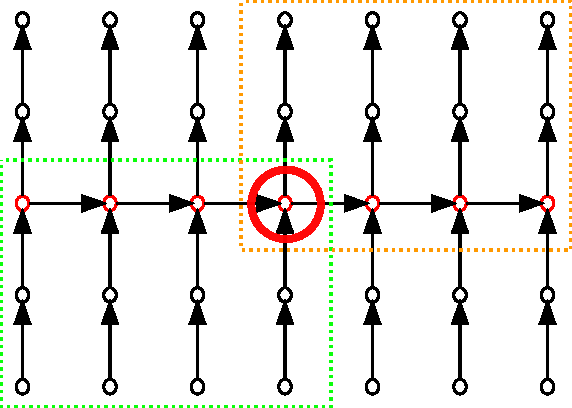
\includegraphics{kap2mediansuche}
  \centering
  \caption{Graphische Darstellung der Mediansuche: von links nach rechts sieht man die fünf\-ele\-men\-ti\-gen Teilfolgen, jeweils von oben nach unten absteigend sortiert (ein Pfeil steht für $\le$). Die roten Punkte markieren die Mediane, der rote Kreis den Median der Mediane. Die \textcolor{green}{grüne} Box markiert die Menge A, die alle Elemente enthält von denen aus es einen gerichteten Pfad zum Median der Mediane gibt. Die \textcolor{orange}{orangene} Box markiert die Menge B, die alle Elemente enthält zu denen es einen gerichteten Pfad vom Median der Mediane aus gibt. Beim Aufspalten fällt eine von beiden Mengen weg, so dass der rekursiver Aufruf höchstens die übrigen Elemente untersuchen muss.}
  \label{mediansuche}
\end{figure}

Wenn $n$ kein Vielfaches von 5 ist, können wir neben der letzten fünfelementigen Teilmenge bis zu vier weitere Elemente habe. Diese berücksichtigen wir bei der Mediansuche nicht, sie fließen einfach direkt in die Menge der Elemente ein, die später untersucht werden.

Wir wissen, dass es in Abbildung \ref{mediansuche} einen gerichteten Pfad von allen Elementen der Menge $A$ zu $a$, dem Median der Mediane gibt. Daher gilt $\forall b \in A : b \le a$. Analog können wir folgende Aussage gestalten $\forall b \in B : b \ge a$. Beim Aufspalten bezüglich $a$ fällt daher die Menge $A$ oder die Menge $B$ weg. Der rekursive Aufruf untersucht daher höchstens die restlichen Elemente. Es gibt $\frac{n}{5}$ Teilfolgen, von denen die eine Hälfte zu $A$ beiträgt, die andere Hälfte zu $B$. Jede Teilfolge hat fünf Elemente, von denen wiederum die Hälfte zu $A$ beziehungsweise zu $B$ gehört. Wir können die Größe von $A$ und $B$ somit abschätzen als $|A| \ge \lceil\frac{\lfloor\frac{n}{5}\rfloor}{2} \rceil \cdot 3 = 3 \cdot \lfloor \frac{n}{10} \rfloor \le |B|$.

Die rekursiven Aufrufe betreffen daher höchstens $|S_1|, |S_3| \le n - 3 \lfloor \frac{n}{10} \rfloor$ Elemente. Diese können wir weiter abschätzen: Es gilt $n - 3 \lfloor \frac{n}{10} \rfloor \le n - 3 (\frac{n}{10} - 1) = 0,7 n + 3 \le 0,75 n$ falls $3 \le 0,05 n$ also für hinreichend Große $n \ge 60$. Dies begründet die erste Zeile des Algorithmus, die für die ersten 60 Elemente einen Brute-Force-Ansatz wählt.

Wir erhalten folgende Rekursions(un)gleichung:
\begin{align*}
  T(n) &\le c \qquad\text{für n < 60}\\
  T(n) &\le \underbrace{T(\lfloor\frac{3}{4}n\rfloor)}_{\text{für den Rek. Aufruf}} + \underbrace{T(\lfloor \frac{n}{5} \rfloor)}_{\text{für die Mediansuche}} + \underbrace{dn}_{\text{aufteilen in } S_1, S_2, S_3} + \mathcal{O}(n)
\end{align*}
%Wir erhalten folgende Rekursions(un)gleichung:
%\begin{align*}
%  T(n) &\le c \qquad\text{für n < 60}\\
%  T(n) &\le \underbrace{T(\lfloor\frac{7}{10}n\rfloor)}_{\text{für den Rek. Aufruf}} + \underbrace{T(\lfloor \frac{n}{5} \rfloor)}_{\text{für die Mediansuche}} + \underbrace{dn}_{\text{aufteilen in } S_1, S_2, S_3}
%\end{align*}
%
%Es gilt $n - 3 \lfloor \frac{n}{10} \rfloor \le n - 3 (\lfloor \frac{n}{10} \rfloor-1) = 0,7 n + 3 \le 0,75 n$ falls $3 \le 0,05 n$ also für hinreichend Große $n \ge 60$. Dies begründet die erste Zeile des Algorithmus, die für die ersten 60 Elemente einen Brute-Force-Ansatz wählt. Für hinreichend große $n$ können wir abschätzen $\frac{n}{5} \le \frac{n}{5} +1 \le \lfloor 0,25 n \rfloor$. Wir können also schreiben:
%\[ T(n) \le T(\lfloor\frac{3}{4}n\rfloor) + T(\lfloor \frac{n}{4} \rfloor) + dn \]

Warum ergibt das lineare Laufzeit? Wir zeigen per Induktion, dass es eine Konstante $b$ gibt, so dass $T(n) \le bn$ für alle $n \in \mathbb{N}$ und somit $T(n) \in \mathcal{O}(n)$ liegt.

Betrachten wir zunächst den Induktionsanfang für $n<60$. $T(n) \le c$. Wir wählen die Konstante $b$ nun so, dass gilt $b \ge c$ und der Induktionsanfang somit stimmt.
Es folgt der Induktionsschritt $n-1 \to n$. 
\[ T(n) \le \frac{3}{4} bn + \frac{1}{5} bn + dn = (0,95 b + d) n \]
Wir wählen $b$ nun so, dass $0,95 b + d \le b$, also $d \le 0,05 b$ und somit $20 d \le b$.

$b$ lässt sich ingesammt bestimmen durch $b = max(c, 20 d)$, womit wir gezeigt hätten, dass es eine Konstante $b$ gibt, so dass $T(n) \le bn$ und somit $T(n) \in \mathcal{O}(n)$.

\begin{Satz}[Deterministische Select hat lineare Laufzeit]
\hspace{\parindent}Die deterministische Variante von \textsc{Select} hat auch im schlechtesten Fall eine Laufzeit von $\mathcal{O}(n)$.
\end{Satz}

\section{Suchen}

Gegeben ist eine Menge $S \subset \mathcal{U}$ mit $\mathcal{U}$ linear geordnetem Universum: $(\mathcal{U}, \le)$. Welche Möglichkeiten gibt es $S$ so abzuspeichern, dass eine effiziente Suche in $S$ möglich ist? Mit "`Suche"' ist ein Algorithmus gemeint, der feststellt, ob ein $a \in \mathcal{U}$ in $S$ enthalten ist und gegebenenfalls die Stelle findet, an der sich $a$ in $S$ befindet.

\subsection{Binärsuche}
Eine Lösung ist ein geordnetes Feld für $S$. Diese Datenstruktur ermöglicht Binärsuche.

%\begin{figure}[htb]
%  \centering
%  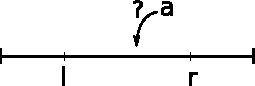
\includegraphics{kap2binsuch}
%  \caption{Ein Beispiel für die Vorgehensweise der Binärsuche.}
%\end{figure}

\begin{Alg}[Binärsuche]
\begin{algorithmic}[1]
\Function{binsuche}{$l$, $r$, $a$}
  \If{$l \le r$}
    \State $k = \frac{l + r}{2}$
    \If{$S[k]==a$}
      \State \textbf{return} $k$
    \ElsIf{$S[k] > a$}
       \State \textbf{return} Binsuche($l$, $k-1$, $a$)
     \Else
       \State \textbf{return} Binsuche($k+1$, $r$, $a$);
    \EndIf
  \Else
    \State \textbf{return} nicht gefunden
  \EndIf
\EndFunction
\end{algorithmic}
\end{Alg}

Betrachten wir die Laufzeit $T(n)$ der Binärsuche, mit $n = |S|$. Der Suchraum wird bei jedem Schritt halbiert. Daher ergibt sich folgende Rekursionsgleichung:
\begin{align*}
  T(1) &= c\\
  T(n) &= T(\lfloor \frac{n}{2} \rfloor) + d
\end{align*}
Daraus folgt $T(n) = \mathcal{O}(\log n)$. Wesentlich effizientere Laufzeit im Mittel weißt die Interpolationssuche auf, die versucht den Suchraum auf den Bereich einzuschränken, in dem ein Treffer erwartet wird.

\subsection{Interpolationssuche}
Nehmen wir an das Universum $\mathcal{U}$ ist ein linear geordnetes Intervall reeller Zahlen, o.B.d.A $\mathcal{U}=[0,1]$. Gehen wir weiter davon aus, dass $S$ unabhängige und gleichverteilte Elemente sind, die zufällig aus $\mathcal{U}$ gewählt wurden.

\begin{Bem}
\hspace{\parindent}Jedes beliebige Intervall lässt sich auf das Intervall $[0,1]$ abbilden und umgekehrt. Aus der Beschränkung folgt lediglich, dass es ein größtes und ein kleinstes Element in $\mathcal{U}$ gibt.\end{Bem}

\begin{figure}[htb]
  \centering
  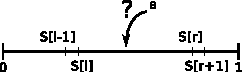
\includegraphics[scale=1.25]{kap2Interpolationssuche}
  \caption{Beispiel: Es soll der Bereich $S[l] \ldots S[r]$ nach $a \in [0,1]$ durchsucht werden, dabei ist $S$ ein aufsteigend sortiertes Feld.}
  \label{interpolationssuche}
\end{figure}

Die Interpolationssuche funktioniert genau wie die Binärsuche, bis auf die Auswahl des Pivotelements $a$. Als Pivotelement wählen wir das $k$-te Element der Folge $S$, wobei $k$ wie folgt definiert ist:
\[ k=l-1 + \left\lceil \frac{a-S[l-1]}{S[r+1]-S[l-1]} \cdot (r-l+1) \right\rceil \]
Wir versuchen also das Element als Pivoelement zu wählen, bei dem wir bei perfekter Gleichverteilung das gesuchte Element erwarten würden.

% 0......S[l-1].S[l]..........S[r].S[r+1]...........1
%           (_________________________)
%                      ^a

%$k=l-1 + \left\lceil \frac{a-S[l-1]}{S[r+1]-S[l-1]} \cdot (r-l+1) \right\rceil$

Möchte man die Rekursionsfolge aufstellen, um die Laufzeit zu berechnen, so sollte man für $S[0] = 0$ und $S[n+1] = 1$ setzen.

Die Laufzeit der Interpolationssuche ist abhängig von der Größe der durchsuchten Folge: $|S|=n$. Im schlechtesten Fall hat die Interpolationssuche eine Laufzeit von $\Theta(n)$, im Mittel liegt die Laufzeit bei $\mathcal{O}(\log\log n)$. Der Beweis der Laufzeit ist zu komplex für diese Veranstaltung.

\subsection{Quadratische Binärsuche}
%           ___ = \sqrt{m}
% ______________________________m   mit m=r-l+1
%...S[l]..||...||...S[k].......S[r]
%                    ^a? sonst
%               ^a? sonst
%          ^a?
Um ein Feldsegment von $S[l]\ldots S[r]$ nach $a \in [0,1]$ zu durchsuchen bestimmen wir das Pivotelement, wie bei der Interpolations-Suche und nennen es $k$. Falls $a=S[k]$ haben wir das gewünschte Element bereits gefunden. Falls $S[k] > a$ überprüfen wir die Elemente $S[k-\sqrt{m}], S[k-2 \sqrt{m}], \ldots , S[k - i \sqrt{m}]$ bis ein Element $\le a$ gefunden wird, wobei $m = r-l+1$. Dann durchsuchen wir rekursiv den Bereich $S[k-i \cdot \lceil\sqrt{m}\rceil] \ldots S[k-(i-1) \cdot \lceil\sqrt{m}\rceil]$. Sollte $a > S[k]$ sein, gehen wir analog vor.

\begin{figure}[hbt]
  \centering
  \includegraphics{kap2quadratischeBinsuche}
  \caption{Quadratische Binärsuche: es wird die erwartete Position von $a$ berechnet. Je nachdem ob der vorgefundene Wert größer oder kleiner ist wird nach links oder rechts um $\sqrt{m}$ Felder gesprungen, bis ein kleinerer/größerer Wert als $a$ gefunden wird. in dem so eingegrenzten Intervall wird dann nach $a$ gesucht.}
  \label{quadratischeBinsuche}
\end{figure}

%$S[k-1\sqrt{m}]$.\\
%durchsuche rekursiv $S[k-i\lceil\sqrt{m}\rceil]...S[k-(i-1) \lceil\sqrt{m}\rceil]$
%Analyse:

\begin{Lza}
\hspace{\parindent}Wie viele Sprünge der Länge $\lceil\sqrt{m}\rceil$ sind im Mittel notwendig um richtiges Intervall der Länge $\lceil\sqrt{m}\rceil$ zu finden? Die Anzahl der Sprünge ist abhängig vom Abstand zwischen der erwarteten Position des gesuchten Elements $a$ und seiner tatsächlichen Position. Die tatsächliche Postion können wir auch mit $rang(a)$ bezeichnen, ihre erwartete Position (den Erwartungswert von $rang(a)$) haben wir mittels $k$ angegeben.

Den Erwartungswert über die der Anzahl der benötigten Sprünge nennen wir $c$. $P_i$ ist die Wahrscheinlichkeit, dass mindestens $i$ Sprünge gebraucht werden um $a$ zu finden. $P_i - P_{i+1}$ entspricht der Wahrscheinlichkeit genau $i$ Sprünge zu brauchen. Wir können dann $c$ berechnen:
\[c = \sum_{i=1}^{\infty} i \cdot (P_i - P_{i+1})\]
Das lässt sich zusammenfassen:
\begin{align*}
  c &= \sum_{i=1}^{\infty} i \cdot (P_i - P_{i+1}) \\
    &= \sum_{i=1}^{\infty} i \cdot P_i - \sum_{j=2}^{\infty} (j-1) \cdot P_{j} \\
    &= P_1 + \sum_{i=2}^{\infty} (i \cdot P_i - (i-1) \cdot P_{i}) \\
    &= \sum_{i=1}^{\infty} P_i %\qquad \text{mit } P_1, P_2 \le 1
\end{align*}

$P_1$ und $P_2$ sind die Wahrscheinlichkeiten, dass mindestens $1$ beziehungsweise mindestens $2$ Sprünge benötigt werden, um $a$ zu finden. Es gilt $P_1, P_2 \le 1$. Bei $i \ge 3$ Sprüngen ist der Rang von $a$ um mindestens $(i-2) \cdot \sqrt{m}$ von seinem Erwartungswert $k$ entfernt, also:
\[ |rang(a) -k| \ge (i-2) \cdot \lceil\sqrt{m}\rceil \]
Also gilt für $i \ge 3$, dass $P_i$ kleiner oder gleich der Wahrscheinlichkeit ist, dass der Abstand zwischen $rang(a)$ und $k$ größer oder gleich $(i-2) \cdot \sqrt{m}$ ist:
\[ P_i \le P(|rang(a) - k| \ge (i-2) \cdot \sqrt{m}) \]

Die Wahrscheinlichkeit, dass der Wert einer Zufallsvariablen sich um mehr als einen gegebenen Wert von dem Erwartungswert dieser Zufallsvariablen unterscheidet, lässt sich mit der Tschebyscheff Ungleichung abschätzen.
\[ P(|X - \mu| \ge t) \le \frac{\sigma^2}{t^2} \]
Dabei ist $X$ die Zufallsvariable und $\mu$ ihr Erwartungswert. $\sigma$ ist die Standardabweichung und $\sigma^2$ ist die Varianz von $X$, das heißt $\sigma^2 (X) = E((X-E(X))^2)$

%$X$ Zufallsvariable und $\mu$ ihr Erwartungswert.
%$\sigma^2$ Varianz von $X = E((X-E(x))^2)$
%$\sigma$ Standardabweichung

\begin{figure}[hbt]
  \centering
  \includegraphics{Suche-Intervall-l_minus_1-r_plus_1}
  \caption{Suche von $a$ über die Teilfolge $S[l] \ldots S[r]$, also über die Werte des Intervalls $\left( S[l-1], S[r+1] \right)$. }
  \label{Suche_Intervall_lr}
\end{figure}

Abbildung \ref{Suche_Intervall_lr} veranschaulicht die Suche von $a$ über der Teilfolge $S[l] \ldots S[r]$, also über die Werte des Intervalls $\left( S[l-1], S[r+1] \right)$. Unsere Zufallsvariable $X(a)$ bildet das gesuchte Element $a$ auf seinen Rang $rang(a)$ ab. Der ist identisch mit der Anzahl der $S[j]$ für die gilt $S[j] \le a$. Wir gehen davon aus, dass $S[j]$ unabhängige, gleichverteilte, gleichmäßig über dem Intervall $(S[l-1], S[r+1])$ gezogene Elemente sind, die nach ihrer Ziehung ihrer Größe nach geordnet wurden. Die Wahrscheinlichkeit, dass ein zufällig aus $(S[l-1], S[r+1])$ gezogenes Element $S[j] \le a$ ist, können wir angeben als
\[ P = \frac{a - S[l-1]}{S[r+1] - S[l-1]} \]
Es ist klar, dass $j = l, \ldots, r$ sein muss. Wir erinnern uns, dass wir $m = r-l+1$ definiert hatten. Nun können wir der Binomialverteilung entsprechend berechnen, wie groß die Wahrscheinlichkeit ist, dass $q$ viele $S[j] \le a$ sind:
\[ \binom{m}{q} \cdot P^q \cdot (1-P)^{m-q} \]

$\binom{m}{q}$ gibt die Möglichkeiten an $q$ Stück aus $m$ auszuwählen. $p^q$ steht für die Wahrscheinlichkeit, dass diese $q$ alle $\le a$ sind. $(1-p)^{q-m}$ entspricht der Wahrscheinlichkeit, dass die restlichen $S[j] >a$ sind.

Der Erwartungswert einer binomialverteilten Größe ist
\begin{align*}
  E(X) &= \mu \\
       &= \sum_{q=0}^{m} q \cdot \binom{m}{q} \cdot P^q \cdot (1-P)^{m-q}\\
       &= P \cdot m
\end{align*}

Ihre Varianz ist
\begin{align*}
  \sigma^2 &= E((X-E(X))^2) \\
           &= E\left(\left(\binom{m}{q} \cdot P^q \cdot (1-q)^{m-q} - P \cdot m\right)^2\right) \\
           &= P \cdot (1-P) \cdot m
\end{align*}

Wir können $P_i$ jetzt durch die Tschebyscheff Ungleichung abschätzen.
\[ \underbrace{P_i}_{\ge i \text{ Sprünge, } i \ge 3} \le \frac{\sigma^2}{t^2} \le \frac{P \cdot (1-P) \cdot m}{((i-2)\sqrt{m})^2} = \frac{P \cdot (1-P)}{(i-2)^2} \]

\begin{figure}[htb]
	\centering
	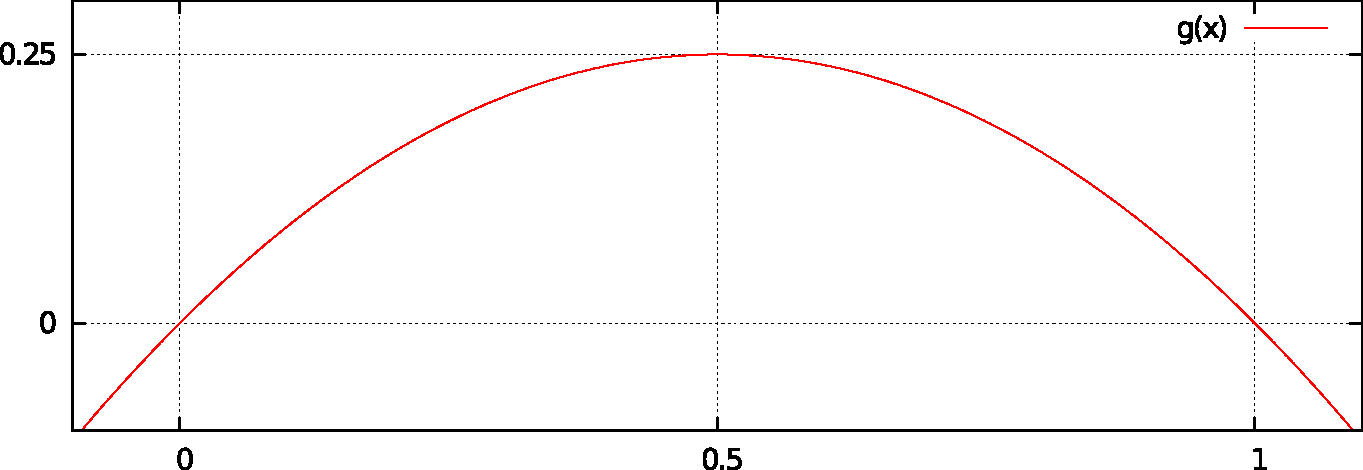
\includegraphics[width=.75 \textwidth]{kap2x-xQuadrat}
	\caption{Visualisierung von $P(1-P)$ zur Abschätzung gegen $0,25$.}
	\label{kap2x-xQuadrat}
\end{figure}

Abbildung \ref{kap2x-xQuadrat} visualisiert $P(1-P)$. Es ist leicht zu sehen, dass wir $P(1-P) \le \frac{1}{4}$ setzen können, also $P_i = \frac{P \cdot (1-P)}{(i-2)^2} \le \frac{1}{4 \cdot (i-2)^2}$.

Nun lässt sich die erwartete Anzahl von Vergleichen genau bestimmen. Weil $P_1, P_2 \le 1$ können wir $P_1+P_2 \le 2$ abschätzen. Dank Gauß wissen wir $\sum_{j=1}^{\infty} \frac{1}{j^2} = \frac{\pi^2}{6}$.

\begin{align*}
	c &= \sum_{i=1}^{\infty} P_i\\
	  &\le 2 + \frac{1}{4} \sum_{i=3}^{\infty} \frac{1}{(i-2)^2} \\
	  &= 2 + \frac{1}{4} \sum_{j=1}^{\infty} \frac{1}{j^2}\\
	  &= 2 + \frac{\pi^2}{24}\\
	  &= 2,411\ldots
\end{align*}

Damit können wir die Rekursionsgleichung für $T(n)$ aufstellen:
\begin{align*}
  T(1) &= b \\
  T(n) &\le T(\sqrt{n}) + c
\end{align*}

$T(\sqrt{n})$ berechnet die Kosten für den rekursiven Aufruf. Den Suchraum kann man im Mittel in konstanter Zeit auf $\sqrt{n}$ einschränken, was durch $c$ (zuvor gegen $2,411\ldots$ abgeschätzt) berücksichtigt wird.

Wir analysieren die Rekursionsgleichung für $n$ der Form $2^{2^k}$.
\begin{align*}
  T(1) &=b \\
  T(n) &\le T(\sqrt{n}) + c \\
       &\le T(n^{\frac{1}{4}}) +2 \cdot c \\
       &\quad\vdots \\
       &\le T(n^{(\frac{1}{2}^a)}) + a \cdot c \\
       &\le T(2) + c \cdot \log \log n
%\\     & = \mathcal{O}(\log \log n)
\end{align*}
$a$ setzen wir also so, dass gilt $n^{\left(\frac{1}{2}^a\right)} = 2$. Daraus folgt:
\begin{align*}
  \log n^{\frac{1}{2^a}} &= 1 \\
  \frac{1}{2^a} \log n &= 1\\
  \log n &= 2^a\\
  \log \log n &= a
\end{align*}
und daher $ T(n) \in \mathcal{O}(\log \log n)$. Für allgemeine $n$ ließe sich durch Induktion zeigen, dass $T(n) \le c \cdot \log \log n$.
\end{Lza}

\chapter{Datenstrukturen}
\begin{Def}[Datenstruktur]
\hspace{\parindent}Eine Datenstruktur definiert eine Art Daten abzuspeichern, damit gewisse Operationen effizient ausgeführt werden können. Bei der Analyse betrachtet man
  \begin{itemize}
    \item die Vorverarbeitungszeit (preprocessing) um die Datenstruktur aufzubauen
    \item den Speicherplatz
    \item Zeit für die Operationen (z.B. Suchen, Einfügen, und so weiter).
  \end{itemize}
\end{Def}

Es gibt Datenstrukturen, in denen man z.B. sehr effizient suchen kann, die aber beim Einfügen oder Löschen vergleichsweise langsam sind. Andere Datenstrukturen sind darauf ausgelegt schnell Daten aufnehmen zu können, eignen sich wiederum nicht so dazu durchsucht zu werden.	

\section{Wörterbuch (dictionary)}
Als Wörterbuch versteht man einen abstrakten Datentyp, der Daten über einem Universum $\mathcal{U}$ in einer Menge $S \subseteq \mathcal{U}$  speichert. Über $\mathcal{U}$ ist meist eine lineare Ordnung definiert, z.B. $\le$.

Operationen auf Datenstrukturen, die man zu Wörterbüchern zählt sind:
\begin{itemize}
  \item \texttt{Suche}($a$, $S$): $a \in S$?
  \item \texttt{Einfügen}($a$, $S$): $S := S \cup \{a\}$
  \item \texttt{Streichen}($a$, $S$): $S := S \setminus \{a\}$
\end{itemize}

Betrachten wir uns einige konkrete Datentypen, die man als Wörterbuch ansehen kann.

\subsection{Sortiertes Feld}
Ein Sortiertes Feld ist sehr effizient, wenn es um das Suchen eines Wertes geht. Die Suche auf einem sortierten Feld lässt sich in $\mathcal{O}(\log n)$ ausführen. Für das Einfügen und Streichen von Elementen wird $\Theta(n)$ Zeit gebraucht.

\subsection{Hashing}
Unter Hashing versteht man ein Feld der Größe $m$ und eine Hashfunktion $h : \mathcal{U}\rightarrow \{ 1, \ldots, m \}$. Mit Hilfe der Hashfunktion wird die Stelle im Feld bestimmt, an der ein Element gespeichert werden soll, beziehungsweise gespeichert ist. $h$ ist im allgemeinen nicht injektiv, das heißt es kann mehrere Elemente in $S$ geben, die auf die gleiche Stelle $i$ abgebildet werden, ein entsprechendes Beispiel zeigt Abbildung \ref{kap3hashfunktion}.

\begin{figure}[htb]
  \centering
  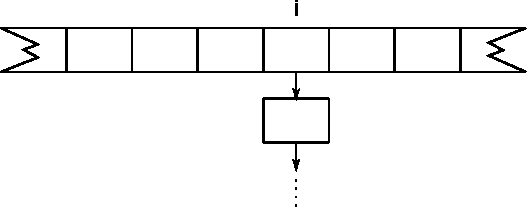
\includegraphics[scale=.8]{kap3hashfunktion}
  \caption{Die Hashfunktion ist meist nicht injektiv. Alle Elemente $x$ mit $h(x) = i$ werden in einer Liste an Stelle $i$ im Feld gespeichert.}
  \label{kap3hashfunktion}
\end{figure}

Einfügen, Suchen und Streichen kosten $\mathcal{O}(1 + \text{Länge der Liste})$ Zeit. Zumindest im Mittel $\mathcal{O}(1)$, falls es gelingt Listenlänge konstant zu halten.

Bei einem Array, wie es in Abbildung \ref{kap3hashfunktion} dargestellt wird, möchte man nicht zu viel Platz verschwenden. Entsprechende Anforderungen sind an die Hashfunktion zu stellen. Wählt man ein Element aus $\mathcal{U}$ zufällig, so sollte jede Position, die die Hashfunktion für das Element berechnet, gleich wahrscheinlich sein.

Man kann die mittlere Listenlänge auch bei beliebig vielen Einfügungen konstant halten. Sobald das Verhältnis  $\frac{|S|}{m}$ eine Konstante (zum Beispiel 2) übersteigt verdoppelt man die Anzahl der Plätze $m$ und fügt alles in das neue Feld ein. Eine einzelne Einfügung kann so zwar $\Theta(n)$ Zeit kosten, aber amortisiert über alle Einfügeoperationen erhalten wir eine Laufzeit von $\mathcal{O}(1)$.

\subsection{Binäre Suchbäume}
Ein Binärer Suchbaum ist eine Datenstruktur, bei der die Elemente in Knoten eines Baums angeordnet werden. Alle Kinder $k$ eines Knotens $a$, für die gilt $k \le a$, werden dem linken Teilbaum der Nachfolger von $a$ hinzugefügt, alle anderen Knoten dem rechten. Abbildung \ref{kap3Suchbaum} stellt das für einen Knoten und zwei Teilbäume dar.

\begin{figure}[hbt]
  \centering
  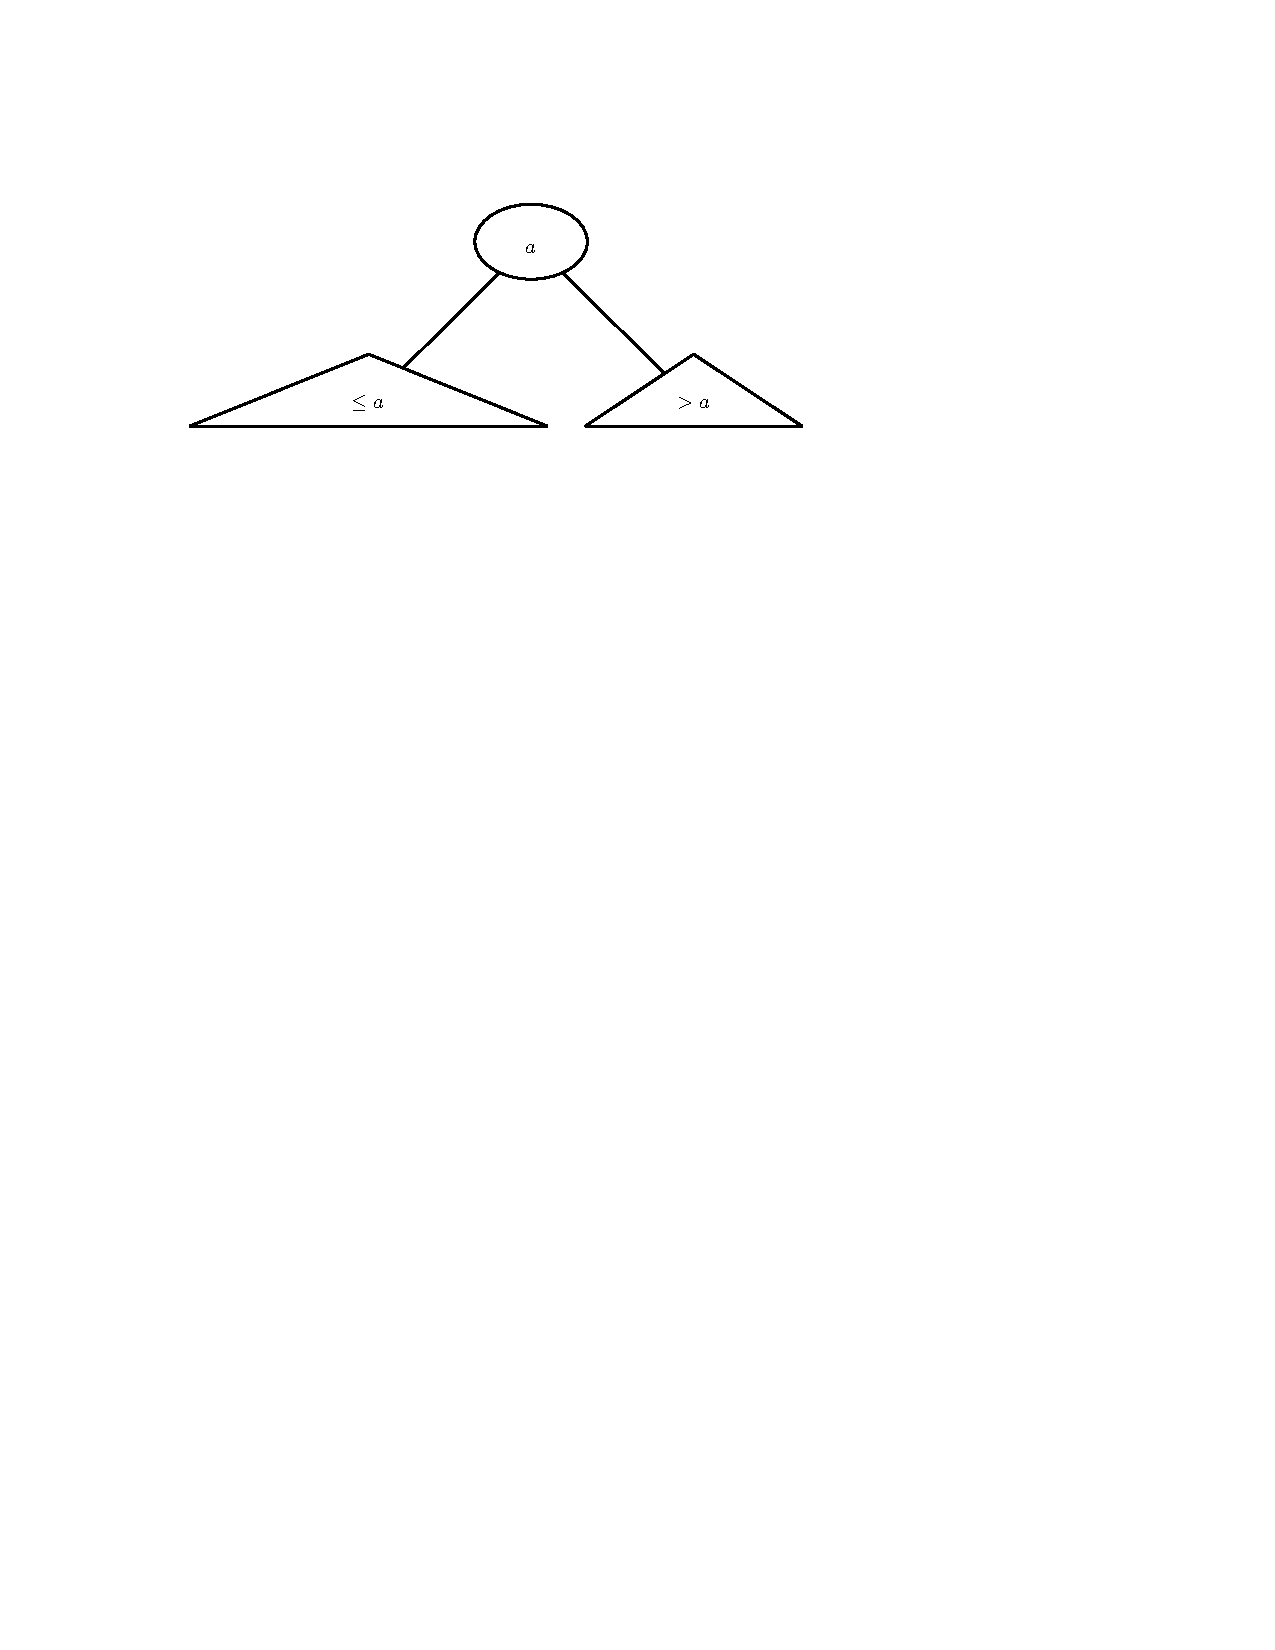
\includegraphics[scale=.75]{kap3Suchbaum}
  \caption{Jeder Knoten eines binären Suchbaums hat maximal zwei Kinder. Alle Kinder, die im linken Teilbaum angehängt sind, sind kleiner oder gleich als der Knoten $a$. Alle Kinder von $a$ die größer sind, werden zum rechten Teilbaum hinzugefügt.}
  \label{kap3Suchbaum}
\end{figure}

Die in Abbildung \ref{kap3Suchbaum} dargestellte Strukturierung gilt für jeden Teilbaum eines binären Suchbaums. Die Blätter eines binären Suchbaums enthalten keine Elemente von $S$. Jedes Blatt entspricht einer erfolglosen Suche.

Gesucht wird, in dem das gesuchte Elemente mit der Wurzel des Baums oder eines Teilbaums verglichen wird. Ist sie das gesuchte Element, kann die Suche erfolgreich beendet werden. Andernfalls wird rekursiv im linken oder rechten Teilbaum weiter gesucht, je nachdem, ob der zu vor betrachtete Knoten größer oder kleiner als das gesuchte Element war. Erreicht man ein Blatt des Baums, wird die Suche erfolglos beendet.

Zum Einfügen sucht man nach dem Element, das eingefügt werden soll, bis man ein Blatt erreicht. Anstelle des Blatts fügt man das Element ein und hängt an es zwei neue Blätter an. Beim Streichen sucht man das zu streichende Element und ersetzt es durch die Wurzel des linken Teilbaums seiner Nachfolger.

Suchen, Einfügen und Streichen von Elementen in einem binären Suchbaum lassen sich in $\mathcal{O}(h)$ Zeit realisieren, wobei $h$ für die Höhe des Baums steht. $h$ ist im günstigsten Fall (perfekt ausbalancierter Binärbaum) $\lceil \log n \rceil$ und im schlechtesten Fall (nicht ausbalancierter, entarteter Binärbaum) $n$.

Wie kann man Höhe $\mathcal{O}(\log n)$ garantieren, bei beliebigen Einfügungen und Streichungen? Dazu gibt es viele Ansätze, diese Fragestellung ist gerade in den 1970er Jahren viel untersucht worden. Wir betrachten hier zwei Methoden, die die Höhe $\mathcal{O}(\log n)$ garantieren.

\subsection{Höhenbalancierte Bäume (AVL-Bäume)}
Höhenbalancierte Bäume wurden 1962 von Addson-Velski und Landis vorgestellt, sie werden auch AVL-Bäume genannt. Höhenbalancierte Bäume sind binäre Suchbäume, wobei sich die Höhe des linken und die Höhe des rechten Teilbaums eines jeden inneren Knotens um höchstens 1 unterscheiden.

\begin{Beh}
\hspace{\parindent}Die Höhe eines AVL-Baums mit $n$ inneren Knoten ist $\Theta(\log n)$.
\end{Beh}
\begin{Bew}
\hspace{\parindent}$n_h$ sei die Mindestknotenanzahl eines AVL-Baums der Höhe $h$, also die Mindestanzahl innerer Knoten, mit der die Invariante von AVL-Bäumen erfüllt werden kann. In Abbildung \ref{kap3Mindestknotenzahl1} sehen wir drei Bäume unterschiedlicher Höhe und ihre Mindestkontenanzahl.

\begin{figure}[hbt]
  \centering
  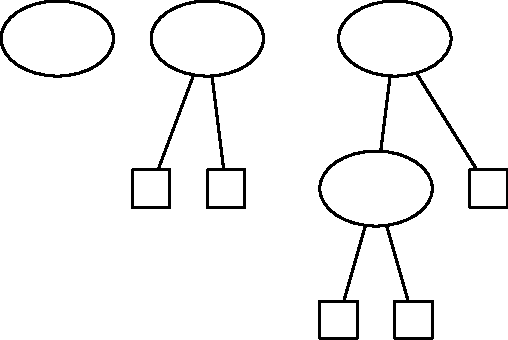
\includegraphics[scale=0.7]{kap3Mindestknotenzahl1}
  \caption{Drei AVL-Bäume mit $n_0 = 0$, $n_1 = 1$, $n_2 = 2$.}
  \label{kap3Mindestknotenzahl1}
\end{figure}

Wir wir in Abbildung \ref{kap3Mindestknotenzahl2} sehen, lässt sich eine Rekursionsgleichung für die Mindestknotenanzahl eines AVL-Baums abhängig von seiner Höhe aufstellen:
\[ n_h = n_{h-1} + n_{h-2} + 1 \]

\begin{figure}[hbt]
  \centering
  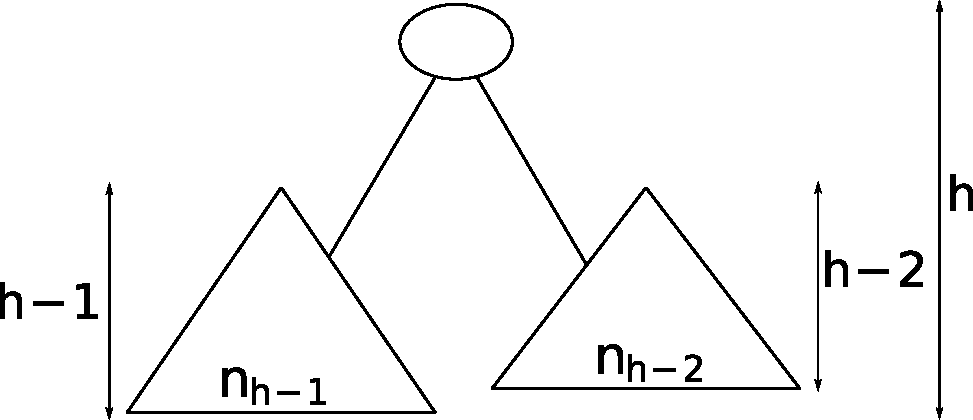
\includegraphics[scale=0.5]{kap3Mindestknotenzahl2}
  \caption{Wenn wir die kleinste Anzahl an inneren Knoten eines AVL-Baumes betrachten, muss der linke Teilbaum $h-1$ Höhe haben, der rechte Teilbaum $h-2$.}
  \label{kap3Mindestknotenzahl2}
\end{figure}

Dies erinnert uns an die Fibonacci-Zahlen. Es gilt $n_h \ge f_{h-1}$ mit $h \ge 1$ und $f_n$ die $n$-te Fibonacci-Zahl. Wir wollen das durch Induktion beweisen. Für den Induktionsanfang mit $h=1$ und $h=2$ gilt dies, wie wir in Abbildung \ref{kap3Mindestknotenzahl1} sehen. Auch der Induktionsschritt ist einfach:
\[ n_h \quad=\quad n_{h-1} + n_{h-2} + 1 \quad\ge\quad f_{h-2} + f_{h-3} + 1 \quad=\quad f_{h-1} + 1 \quad\ge\quad f_{h-1} \qquad \surd \]

Wir wissen, dass $f_{h-1} \ge \phi^{h-2}$. Dabei ist $\phi = \frac{\sqrt{5} +1}{2}$ der sogenannte "`goldene Schnitt"'. Nun können wir $h$ besser abschätzen:
\begin{align*}
  n_h &\ge \phi^{h-2} \\
  \log n_h &\ge (h-2) \log \phi \\
  h &\le \frac{1}{\log \phi} \log n_h +2 \\
%  h &\le \underbrace{\frac{1}{\log \phi}}_{\in [1,2]} \log n_h +2 \\
  h &\le 1,44 \log n_h + 2\\
  h &= \mathcal{O}(\log n_h)\\
  &\Rightarrow \mathcal{O}(\log n) \qquad\text{mit n Anzahl der Knoten}
\end{align*}
\end{Bew}

\begin{figure}[htb]
  \centering
  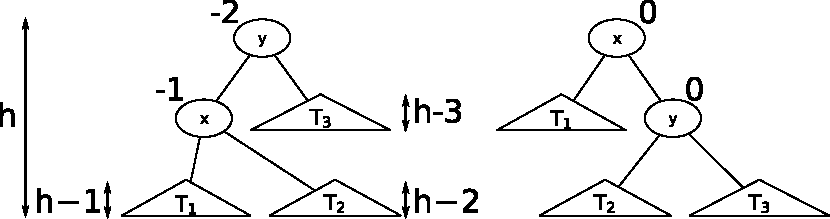
\includegraphics[width=.75\textwidth]{kap3Rotation1}
  \caption{Eine Rotation hilft beim Erhalt der AVL-Eigenschaft. Der Knoten $x$ wird zur neuen Wurzel, sein rechter Teilbaum wird links an $y$ gehangen. Die Zahlen bei den Knoten geben den Wert wieder, den man erhält, wenn man die Höhe des rechten von der Höhe ihres linken Teilbaums abzieht.}
  \label{kap3Rotation1}
\end{figure}

\begin{figure}[hbt]
  \centering
  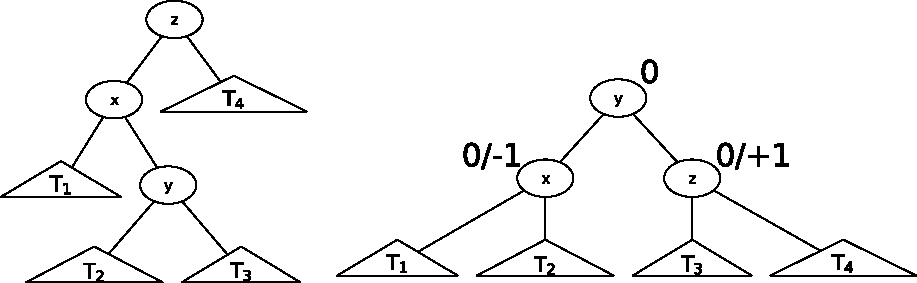
\includegraphics[width=.75\textwidth]{kap3Rotation2}
  \caption{Eine Doppelrotation kann die AVL-Eigenschaft nach dem Löschen oder Hinzufügen weiterer Elemente wieder herstellen.}
  \label{kap3Rotation2}
\end{figure}

Beim Einfügen und Streichen kann die AVL-Eigenschaft verloren gehen. Knoten, die auf dem Suchpfad vom gestrichenem oder eingefügtem Element zur Wurzel liegen, könnten außer Balance geraten. Um das zu verhindern gibt es Operationen, die die AVL-Eigenschaft wieder herstellen. In Abbildung \ref{kap3Rotation1} wird eine Rotation dargestellt, in Abbildung \ref{kap3Rotation2} eine Doppelrotation. Außerdem gibt es weitere symmetrische Fälle, diese beiden Operationen.

Jede solche Operation ist in $\mathcal{O}(1)$ Zeit durchführbar, sie müssen höchsten entlang eines Weges im Baum durchgeführt werden. Daraus folgt $\mathcal{O}(\log n)$ Zeit für die Rebalancierung, da ein Pfad höchstens diese Länge haben kann.

\begin{Satz}
\hspace{\parindent}Suchen, Einfügen und Streichen in AVL-Bäumen ist in $\mathcal{O}(\log n)$ Zeit möglich.
\end{Satz}

Ein AVL-Baum speichert die Daten, sowie jeweils noch zwei Zeiger für das rechte und das linke Kind. Ein AVL-Baum braucht somit $\mathcal{O}(n)$ Speicherplatz. Die Vorverarbeitungszeit liegt in $\mathcal{O}(n \log n)$, da das sortierte Ausgeben eines Baumes nicht besser sein kann, als $\Omega(n \log n)$ und die Ausgabe eines AVL-Baums in linearer Zeit geht.

\subsection{(a, b)-Bäume}
$(a, b)$-Bäume sind Mehrweg Suchbäume. Dabei sind $a, b \in \mathbb{N}$. Des Weiteren gilt $a \ge 2$ und $b \ge 2a -1$.

\begin{Def}
  \begin{figure}[htb]
    \centering
    \includegraphics[width=.8\textwidth]{kap3ABBaum}
  	\caption{Schematische Darstellung eines $(a,b)$-Baums, der in seinen inneren Knoten das Maximum seiner Teilbäume speichert.}
  	\label{kap3ABBaum}
  \end{figure}

\hspace{\parindent}Ein $(a, b)$-Baum ist ein Baum, in dessen Blättern die Menge $S = \{a_1, \ldots, a_n\} \subset \mathcal{U}$ mit $(\mathcal{U}, \le)$ abgelegt ist. Dabei werden folgende Bedingungen erfüllt:
\begin{itemize}
  \item alle Blätter haben gleiche Tiefe
  \item $\delta(v) \le b$ für alle Knoten v, wobei $\delta(v)$ die Anzahl der Kinder von $v$ angibt.
  \item $\delta(v) \ge a$ für alle Knoten von v
  \item $\delta(w) \ge 2$ für die Wurzel $w$
  \item Elemente von $S$ werden in den Blättern von links nach rechts aufsteigend sortiert gespeichert
  \item in jedem inneren Knoten $v$ stehen Elemente $y1 < y2 < \ldots < y_k$ mit $a-1 \le k \le b-1, k = \delta(v) -1$, so dass $y_i$ größtes Element im i-ten Unterbaum von $v$ (siehe Abbildung \ref{kap3ABBaum})
\end{itemize}
\end{Def}

\begin{figure}[htb]
  \centering
  \includegraphics[width=.8\textwidth]{kap3ABWochentage}
  \caption{Beispiel für einen $(2, 3)$-Baum, der die Wochentage enthält.}
  \label{kap3ABWochentage}
\end{figure}

Angenommen die Höhe eines $(a, b)$-Baums sei $h$. Sei $n$ die Zahl der Blätter des $(a,b)$-Baums. Wir können $n$ nun abschätzen. Die Maximale Zahl von Blättern ist $b^h$, genau dann, wenn alle inneren Knoten Grad $b$ haben. Die Minimale Zahl von Blättern ist $2\cdot a^{h-1}$, genau dann, wenn die Wurzel Grad 2 und die anderen Knoten Grad $a$ haben. Wir können also $n$ abschätzen: $2 \cdot a^{h-1} \le n \le b^h$. Daraus folgt:
\[ (h-1) \log a + 1 \le \log n \le h \log b \]
\[ (h-1) \log a       < \log n \le h \log b \]
\[ h=\mathcal{O}(\log n) \]

Betrachten wir nun die Wörterbuchoperationen auf $(a, b)$-Bäumen. Die Suche nach $a \in \mathcal{U}$ verläuft wie folgt: Vergleiche das gesuchte Element mit den Elementen $y_1, \ldots, y_k$, die in der Wurzel gespeichert sind. Ist $a \le y_1$, so wird $i=1$ gesetzt. Ist $a > y_k$, wird $i=k+1$ gesetzt. Andernfalls wird $i$ so gewählt, dass gilt $y_{i-1} < a \le y_i$. Anschließend wird der $i$-te Teilbaum rekursiv durchsucht. Der Baum muss einmal durchlaufen werden, das geschieht in $\mathcal{O}(h) = \mathcal{O}(\log n)$ Zeit.

%Suchen nach $a \in \mathcal{U}$}
%Vergleiche mit den Einträgen $y_1, \ldots, y_k$ in der Wurzel und finde $i$ mit $y_{i-1} < a \le y_i$ (bzw. $a \le y_1$, dann $i=1$ oder $a > y_k$, dann $i=k+1$). Durchsuche rekursive $i$-ten Teilbaum. $\mathcal{O}(1)$ Zeit, weil $a \le k$ und $k$ Konstante. Insgesamt $\mathcal{O}(h) = \mathcal{O}(\log n)$ Laufzeit.

Soll Element $a \in \mathcal{U}$ in einen $(a,b)$-Baum eingefügt werden, so muss die Position gefunden werden, an der ein Blatt mit Inhalt $a$ erwartet wird. Falls es nicht vorhanden ist, hängen wir ein neues Blatt mit Beschriftung $a$ an der entsprechenden Stelle an den Vaterknoten an. Hat der Vaterknoten nun $b+1$ Blätter, müssen wir ihn in zwei Knoten Spalten und überprüfen, ob der Vaterknoten des Vaterknotens dadurch zu viele Kinder hat. Dieser Vorgang setzt sich gegebenenfalls rekursiv bis zur Wurzel fort. Wird die Wurzel gespalten muss eine neue Wurzel erstellt werden, die als Kinder die Knoten enthält, die aus der Spaltung der Wurzel entstanden sind. Eine entsprechende Operation zeigt Abbildung \vref{kap3Einfuegen}.

\begin{figure}[htbp]
  \centering
  \subfloat[Es wird ein Blatt erstellt und eingefügt, der Vaterknoten hat nun jedoch mehr als $3$ Nachfolger, was in einem $(2,3)$-Baum nicht zulässig ist.]{\label{kap3EinfuegenA}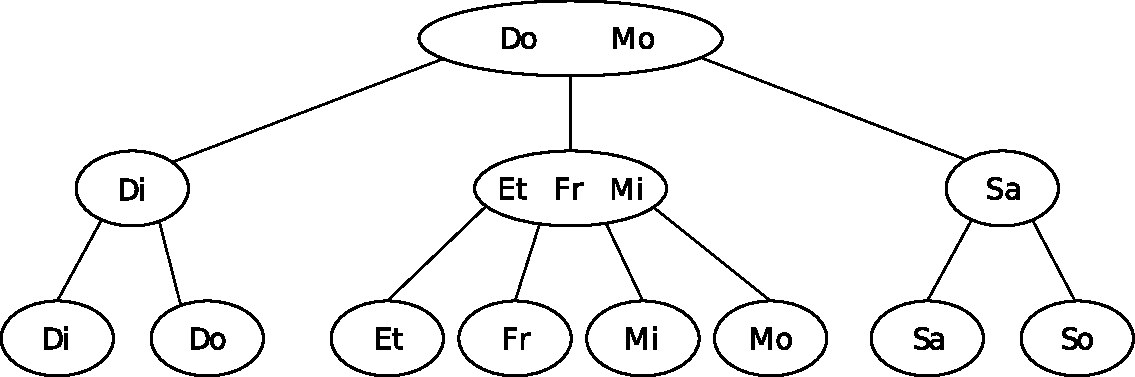
\includegraphics[width=.95\textwidth]{kap3ABEinfuegenA}}
  
  \subfloat[Wir spalten den Vaterknoten und ergänzen die Wurzel um ein Element.]{\label{kap3EinfuegenB}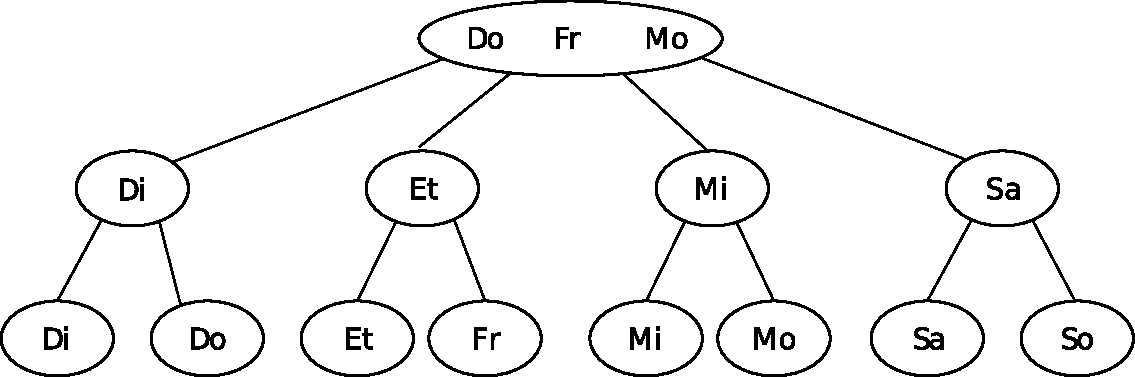
\includegraphics[width=.95\textwidth]{kap3ABEinfuegenB}}
  
  \subfloat[Auch die Wurzel muss gespalten werden. Dazu wird eine neue Wurzel erstellt, die als Kinder die Knoten enthält, die durch die Spaltung der alten Wurzel entstanden.]{\label{kap3EinfuegenC}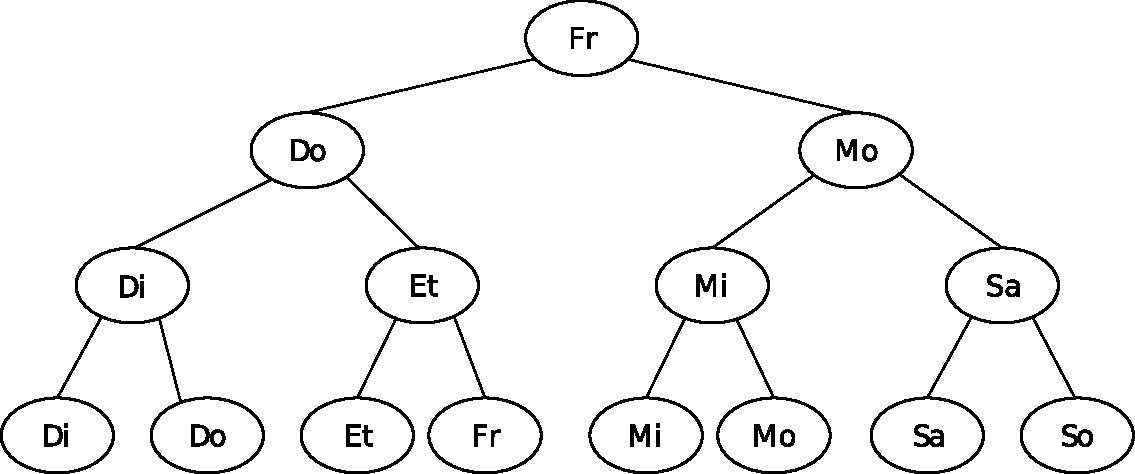
\includegraphics[width=.95\textwidth]{kap3ABEinfuegenC}}
  \caption{Wir fügen den fiktiven "`Etag"' (Et) in den $(2,3)$-Baum aus Abbildung \vref{kap3ABWochentage} ein.}
  \label{kap3Einfuegen}
\end{figure}

%Streichen von $a \in \mathcal{U}$
%Suchen nach a. Falls Blatt mit $a$ gefunden, entfernen wir dieses. Aktualisieren der Einträge der inneren Knoten. Ggf. Zusammenfassen von Knoten.

%Vorlesung 8

Um ein Element $a \in \mathcal{U}$ aus einem $(a,b)$-Baum zu entfernen, müssen wir das Element zu erst im Baum suchen. War die Suche erfolgreich, wird das Blatt dass $a$ enthält entfernt. Hat der Vater $v$ des Blattes nun weniger als $a$ Kinder, müssen wir weitere Operationen vornehmen, um die Invariante von $(a,b)$-Bäumen aufrecht zu erhalten. Wir unterscheiden dabei zwei Fälle:

Im ersten Fall hat der $v$ einen benachbarten Geschwisterknoten $w$, der mehr als $a$ Kinder hat. $v$ kann dann eines der äußeren Kinder von $w$ adoptieren, in die Kante zwischen dem entsprechenden Kind und $w$ gelöst und eine Kante zwischen $v$ und dem Kind erstellt wird. Anschließend sind nur noch die Beschriftungen der inneren Knoten zu aktualisieren.

Im zweiten Fall haben alle benachbarten Geschwisterknoten von $v$ nur $a$ Kinder. In diesem Fall verschmelzen wir $v$ und $w$ zu $v'$. Es kann jetzt sein, dass der Vater von $v$ und $w$ zu wenig Kinder hat und wir die Operation rekursiv fortsetzen müssen. Im schlimmsten Fall müssen wir die Kinder der Wurzel zu einer neuen Wurzel verschmelzen und die alte Wurzel entfernen. Pro Knoten braucht das konstante Zeit, insgesamt liegt die Operation damit bei $\mathcal{O}(h)$, wobei $h$ wieder die Höhe des Baumes bezeichnet. Die Operation liegt also auch in $\mathcal{O}(\log n)$.

\begin{Satz}
  \hspace{\parindent}Suchen, Einfügen, Streichen in $(a,b)$-Bäumen kostet jeweils $\mathcal{O}(\log n)$ Zeit.
\end{Satz}

\subsubsection{Amortisierte Analyse der Zahl der Spaltungen, Adoptionen und Verschmelzungen eines (a,b)-Baumes}
\begin{Beh}
  \hspace{\parindent}Werden in einem leeren $(a,b)$-Baum, mit $b \ge 2a + 1$, $n$ Einfügungen und/oder Streichungen vorgenommen, so ist die Gesamtzahl der SAV"=Operationen (Spaltungen, Adoption, Verschmelzung) höchstens $2n$. Das heißt gemittelt über alle Einfügungen und Streichungen gibt es $\mathcal{O}(1)$ SAV"=Operationen.
\end{Beh}

\begin{Bew}[mittels "`Buchhaltermethode"' (accounting method)]
  \hspace{\parindent}Für jede Einfügung/Streichung werden 2 \euro{} bezahlt. Jede SAV"=Operation kostet 1 \euro{}. Wenn am Schluss keine Schulden entstanden sind, kann es höchstens $2n$ SAV"=Operationen gegeben haben.
  
  Um das zu zeigen, gehen wir davon aus, dass jeder innere Knoten ein Konto hat, auf das das eingezahlte Geld überwiesen wird. Wir betrachten das hier Beispielhaft für einen $(2,5)$-Baum. In einem solchen Baum hat ein innerer Knoten $2, 3, 4$ oder $5$ reguläre Kinder. Beim Löschen oder Einfügen kann ein innerer Knoten vor den Operationen zum ausbalancieren des Baums auch $1$ oder $6$ Kinder haben.

  Wir stellen folgende Invariante über den Kontostand eines inneren Knotens auf:
  \begin{center}
    \begin{tabular}{l|llllll}
      Anzahl der Kinder & 1 & 2 & 3 & 4 & 5 & 6\\\hline
      Kontostand in \euro{} (mindestens) & 3 & 1 & 0 & 0 & 1 & 3
    \end{tabular}
  \end{center}
  
  Betrachten wir nun die SAV"=Operationen und überprüfen wir, ob die Invariante aufrecht erhalten werden kann. Einfüge-Operationen veranschaulicht Abbildung \vref{kap3BuchhalterA}. Streichungen veranschaulicht Abbildung \vref{kap3BuchhalterB}.

\begin{figure}[hbtp]
  \centering
  \subfloat[Einfügen eines Knotens ohne Aufspaltung erhält die Invariante Aufrecht, solange  $-1 \le c \le 2$. Da jede Einfüge"=Operation 2 \euro{} mitbringt, ist das erfüllt.]{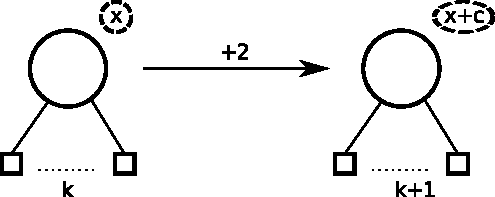
\includegraphics{kap3BuchhalterA1}}
  
  \subfloat[Wird ein Knoten gespalten, so muss er $b+1$ Nachfolger haben. Gemäß der Invariante hat er in einem $(2,5)$-Baum also $3$ \euro{}, die beiden neuen Knoten haben je $0$ \euro{}. Von den drei Euro wird einer auf die Kosten der Operation verwendet, die beiden verbleibenden werden dem Vaterknoten gegeben, da diesem ja ein neuer Knoten hinzugefügt wird. Die Invariante bleibt also erfüllt.]{\includegraphics{kap3BuchhalterA2}}
  
  \subfloat[Muss die Wurzel gespalten werden, entstehen in einem $(2,5)$-Baum zwei neue Knoten mit je 3 Kindern, die nach der Invariante $0$ \euro{} auf dem Konto haben. Die neue Wurzel hat $2$ Kinder und braucht daher $1$ \euro{}. Das Spalten kostet $1$ \euro{}. Die alte Wurzel hatte $6$ Kinder und laut der Invariante entsprechend $3$ \euro{}. Bei der Spaltung der Wurzel ist also sogar ein Euro mehr vorhanden, als erforderlich.]{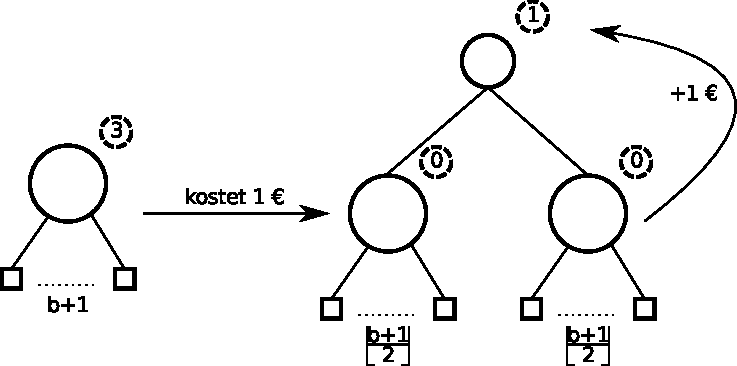
\includegraphics{kap3BuchhalterA3}}
  
  \caption{SAV"=Operationen und Invariante beim Einfügen. In den gestrichelten Kreisen wird der Kontostand der Knoten gezeigt. $c$ schätzt die Kosten der Operation ab.}
  \label{kap3BuchhalterA}
\end{figure}

\begin{figure}[hbtp]
  \centering
  \subfloat[Der Kontostand eines Knotens, dem ein Nachfolger gestrichen wird, verändert sich gemäß der Invariante um $-1 \le c \le 2$. Jede Streichung bringt $2$ \euro{} mit, so dass die Invariante erfüllt bleibt.]{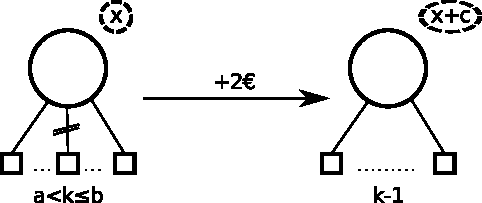
\includegraphics{kap3BuchhalterB1}}
  
  \subfloat[Adoption eines Kindes: wird ein Kind von einem Knoten entfernt, da er von einem Nachbarn adoptiert wird, verändert sich der Kontostand des Knotens um $0 \le c \le 1$ \euro{}. Ein Knoten, der ein Kind adoptieren muss, hat $3$ \euro{}. Einer verbleibt bei ihm, einer deckt die Kosten der Adoption, einer steht zur Verfügung um die Änderung am Kontostand des Nachbarn auszugleichen.]{\includegraphics{kap3BuchhalterB2}}
  
  \subfloat[Verschmelzen zweier Knoten: Wir haben zwei benachbarte Knoten, einen mit einem Nachfolger, einen mit $2$ Nachfolgern. Gemäß der Invariante stehen uns also $4$ \euro{} zur Verfügung. Ein Euro wird auf die Operation an sich verwandt. Der Vaterknoten hat nun ein Kind weniger, sein Kontostand verändert sich also um $-1 \le c \le 2$ \euro{}. Selbst im schlimmsten Fall haben wir daher einen Euro mehr, als wir brauchen, um die Invariante aufrecht zu erhalten.]{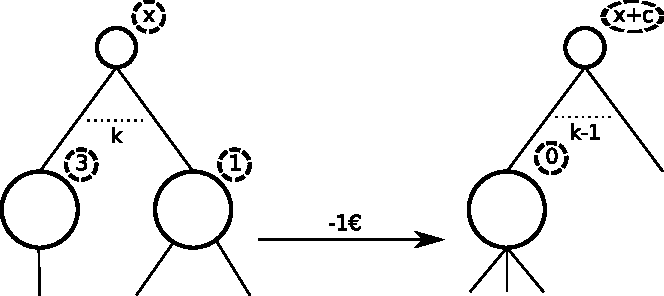
\includegraphics{kap3BuchhalterB3}}
  
  \caption{SAV"=Operationen und Invariante beim Löschen. In den gestrichelten Kreisen wird der Kontostand der Knoten gezeigt.}
  \label{kap3BuchhalterB}
\end{figure}
\end{Bew}

Wir haben also für einen $(2,5)$-Baum bewiesen, dass die Anzahl der SAV"=Operationen bei $n$ Einfügungen/Streichungen $2n$ nicht übersteigt und es somit gemittelt über alle Einfügungen und Streichungen $\mathcal{O}(1)$ SAV"=Operationen gibt.

Es gibt noch andere Datenstrukturen mit $\mathcal{O}(\log n)$ für Wörterbuch Operationen.

\subsection{Rot-Schwarz-Bäume}
Rot-Schwarzbäume sind binäre Suchbäume, in denen die Knoten rot und schwarz gefärbt werden. Rot-Schwarz-Bäume weisen folgende Eigenschaften auf:
\begin{itemize}
  \item alle Blätter und die Wurzel sind schwarz
  \item rote Knoten haben 2 schwarze Kinder
  \item Jeder Weg von der Wurzel bis zu einem Blatt hat gleich viele schwarze Knoten.
\end{itemize}

\begin{figure}[htb]
  \centering
  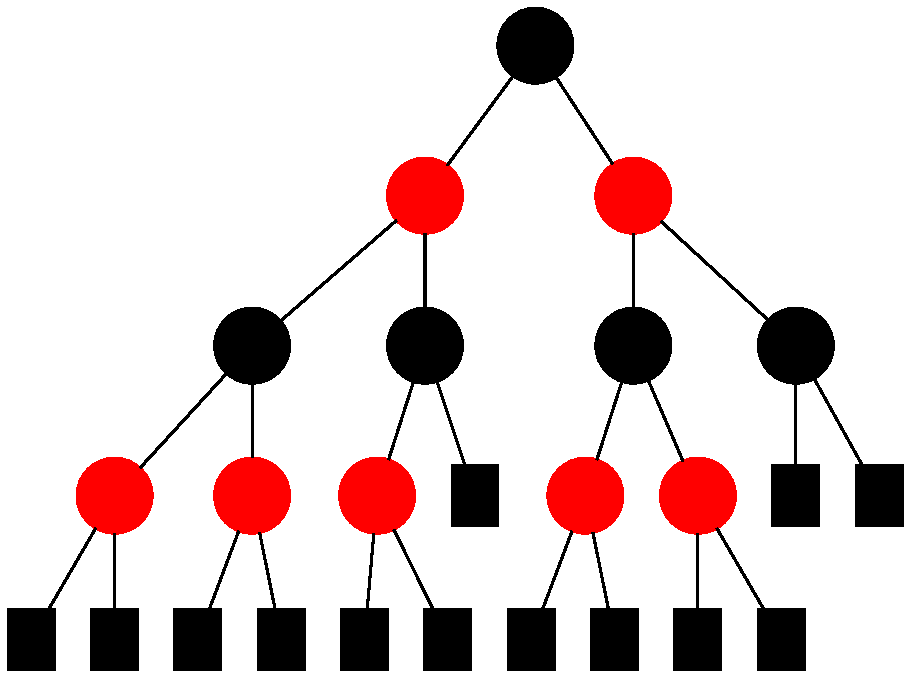
\includegraphics[scale=.6]{kap3RSBaum}
  \caption{Beispiel: Ein Rot-Schwarz-Baum}
  \label{RSBaum}
\end{figure}

Die Höhe eines Rot"=Schwarz"=Baums liegt in $\mathcal{O}(\log n)$, wobei $n$ die Anzahl der Elemente entspricht, die der Rot-Schwarz-Baum enthalten soll. % Genau wie bei B-Bäumen sind diese in den Konten gespeichert, die Höhe eines Rot"=Schwarz"=Baums entspricht also der logarithmischen Anzahl seiner Blätter. % B-Bäume sind (a,b)-Bäume und speichern die Werte nicht in den Knoten sondern in den Blättern (im Gegensatz zu R-S-Bäumen)

Wenn man rote Knoten eines Rot"=Schwarz"=Baums mit ihren schwarzen Vätern verschmilzt, erhält man einen $(2,4)$-Baum.

\subsection{Gewichtsbalancierte Bäume}
Gewichtsbalancierte Bäume werden auch $BB[\alpha]$"=Bäume genannt. Bei $BB[\alpha]$"=Bäumen handelt es sich um binäre Suchbäume.

\begin{figure}[htb]
  \centering
  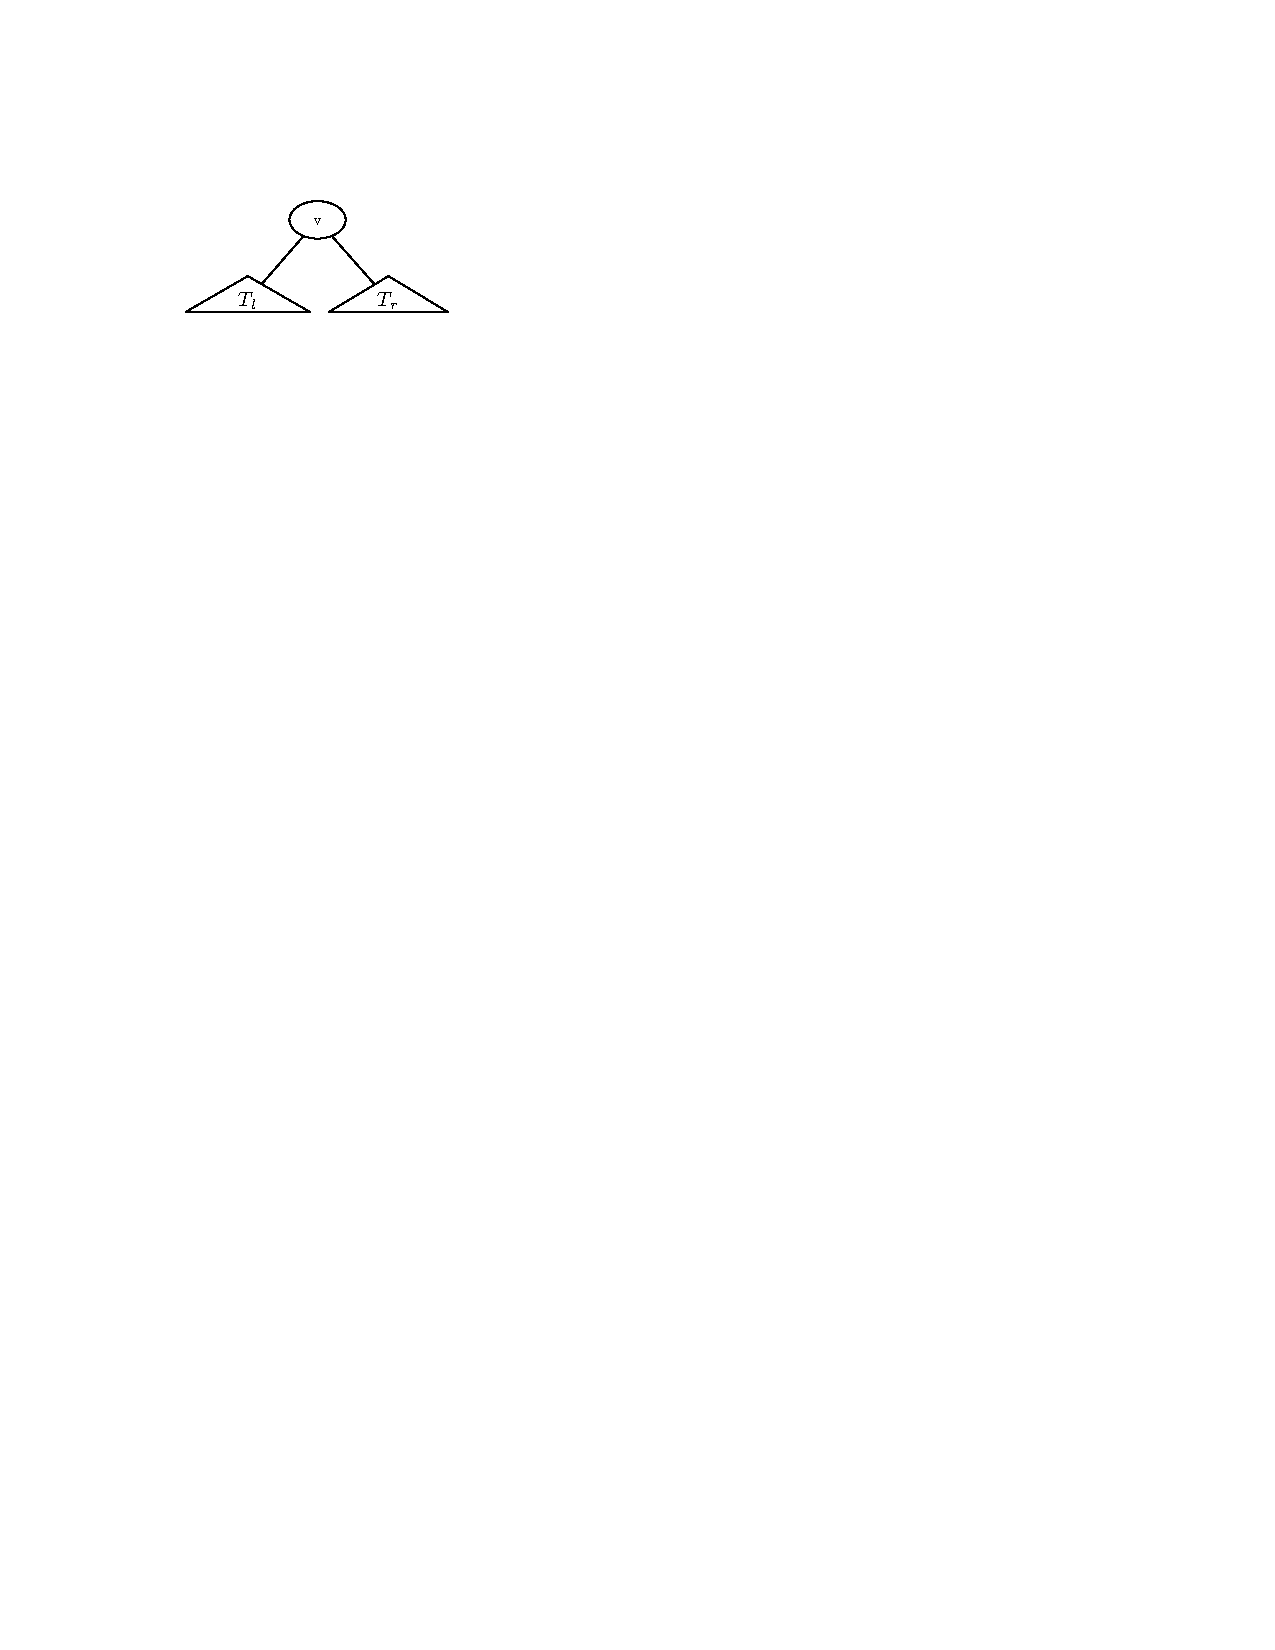
\includegraphics{kap3BBalpha}
  \caption{$balance(v) = \frac{\text{Anzahl der Blätter in } T_l}{\text{Anzahl der Blätter in } T}$}
\end{figure}

\begin{Def}[{$BB[\alpha]$-Baum}]
\hspace{\parindent}Ein $BB[\alpha]$-Baum ist ein binärer Suchbaum mit $\alpha \in (0, \frac{1}{2}]$, $balance(v) \in [\alpha, 1-\alpha]$ für jeden inneren Knoten $v$.
\end{Def}

Es gilt:
\begin{enumerate}
  \item $BB[\alpha]$-Bäume haben logarithmische Tiefe für $0 < \alpha \le \frac{1}{2}$
  \item falls $\alpha \in \left[ \frac{1}{4}, 1-\frac{\sqrt{2}}{2} \right]$ kann die $BB[\alpha]$-Eigenschaft nach Einfügungen und Streichungen durch Rotationen und Doppelrotationen wieder hergestellt werden.
\end{enumerate}

Der Beweis ist kompliziert. Wenn man das $\alpha$ zu klein macht, lässt man zu wenig Spielraum für die Rotation. Macht man $\alpha$ zu groß, kann es dazu kommen, dass man die Balance durch Rotationen und Doppelrotationen nicht wieder herstellen kann.

\subsection{Optimale Binäre Suchbäume}
\begin{Def}[optimaler binärer Suchbaum]
  \hspace{\parindent}Ein binärer Suchbaum ist optimal, wenn die erwartete Anzahl an Vergleichen für eine Suchanfrage minimal ist.
\end{Def}

Angenommen wir haben eine statische Menge $S = \{a_1, a_2, \ldots, a_n\}$ aus einem linear geordnetem Universum $(\mathcal{U}, \le)$, also $S \subseteq \mathcal{U}$. Wie sieht ein optimaler binärer Suchbaum aus? Wie sieht also ein binärer Suchbaum aus, der mit möglichst minimaler Anzahl von Vergleichen beantworten kann, ob für ein Element $a \in \mathcal{U}$ auch $a \in S$ gilt?

Für jeden inneren Knoten in einem binären Suchbaum gilt, dass die Schlüssel der Elemente seines linken Teilbaum kleiner oder gleich seines eigenen Schlüssels sind und die Elemente seines rechten Teilbaums größer seines Schlüssels sind. In den Schlüsseln der inneren Knoten speichern wir also alle Elemente der Menge $S$. Die Blätter stehen für erfolglose Suchen, also für die Intervalle zwischen den Schlüsseln in S: $(-\infty, a_1), (a_1, a_2), \ldots, (a_{n-1}, a_n), (a_n, \infty)$.

Sollten sich balancierte Bäume gut eignen, wird sich die Balance von alleine einstellen. Da $S$ statisch ist, finden keine Einfüge"= oder Streiche"=Operationen statt, wir müssen uns also keine Gedanken darüber machen, ob der Baum auszubalancieren ist oder nicht. Die Blätter können also auch unterschiedliche Tiefe haben, wenn sich das als besonders performant herausstellt.

Um zu entscheiden, welcher Knoten, wo angeordnet wird, müssen wir wissen, wie wahrscheinlich es ist, dass nach einem bestimmten Elemente aus $\mathcal{U}$ gefragt wird. Wir betrachten dazu folgende Wahrscheinlichkeiten:
\begin{enumerate}
  \item $p_i$ sei die Wahrscheinlichkeit, dass bei einer Suchanfrage nach $a_i \in S$ gefragt wird.
  \item $q_i$ sei die Wahrscheinlichkeit, dass bei einer Suchanfrage nach $a \notin S$ gefragt wird, mit $a_i < a < a_{i+1}$.
  \item $q_0$ sei die Wahrscheinlichkeit, dass nach $a$ gefragt wird, mit $a < a_1$.
  \item $q_n$ sei die Wahrscheinlichkeit, dass nach $a$ gefragt wird, mit $a > a_n$.
\end{enumerate}

Da wir es mit einer Wahrscheinlichkeitsverteilung zu tun haben gilt:
\[ \sum_{i=1}^n p_i + \sum_{j=0}^n q_j = 1\]

Wir können nun den Erwartungswert der Anzahl an Vergleichen bestimmen. Also die erwartete durchschnittliche Anzahl von Vergleichen, bei einer Anfrage an den Suchbaum. Er setzt sich zusammen aus den Zugriffswahrscheinlichkeiten für ein Element und die Anzahl der Vergleiche, die erforderlich ist, um zu bestimmen, ob das Element zur Menge $S$ gehört oder nicht:
\[ P = \sum_{i=1}^n p_i \cdot (Tiefe(i) + 1) + \sum_{i=0}^n q_i \cdot Tiefe'(i) \]
wobei $Tiefe(i)$ die Tiefe des Knotens $a_i$ angibt und $Tiefe'(i)$ die Tiefe des Blattes mit dem Schlüssel $(a_i, a_i+1)$, beziehungsweise die Tiefe des Blattes $(-\infty, a_0)$ für $i=0$ oder die Tiefe des Blattes $(a_n, \infty)$ für $i=n$. Diese Zielfunktion wollen wir minimieren, um den perfekten Suchbaum zu finden.

Die erste Summe repräsentiert die Suche nach einem Element $a_i \in S$. Sie summiert für alle Elemente aus $S$ das Produkt aus Anfragewahrscheinlichkeit des Elements und die Anzahl der nötigen Vergleichsoperationen zum Finden des repräsentierenden Knotens. Die Anzahl der Verlgeichsoperationen entspricht der Tiefe des Knotens $+1$ für den Vergleich mit der Wurzel.

Die zweite Summe summiert über die übrigen Anfragen. Das sind Anfragen nach Elementen, die nicht in $S$ gespeichert sind. Alle diese Elemente liegen in den Intervallen, die in als Schlüssel der Blätter genutzt werden. Wir können, um die Anzahl der Vergleiche zu ermitteln, also die Zugriffswahrscheinlichkeit auf eines dieser Elemente mit der Tiefe des Blatts multiplizieren, welches das Intervall enthält, in dem das gesuchte Element liegt.

\subsubsection{Drei beispielhafte Suchbäume}


Betrachten wir ein Beispiel. Sei $\mathcal{U} = \{1, 2, 3, 4, 5, 6, 7\}$ und $S = \{2, 5, 6\}$. Nach den Elementen aus $S$ wird mit den Wahrscheinlichkeiten $p_1 = 0{,}3,\quad p_2 = 0{,}2,\quad p_3 = 0{,}1$ gefragt. Die Intervalle zwischen den Elementen in $S$ seien gleich wahrscheinlich, d.h. $q_0 = q_1 = q_2 = q_3 = 0{,}1$. In Abbildung \vref{kap3OptimaleSB} sehen wir drei mögliche Suchbäume.

\begin{figure}[htb]
  \centering
  \subfloat[Baum $T_1$\label{kap3OptimaleSBT1}]{\includegraphics[width=.4\textwidth]{kap3OptimaleSB2}}
  
  \subfloat[Baum $T_2$\label{kap3OptimaleSBT2}]{\includegraphics[width=.3\textwidth]{kap3OptimaleSB1}}\hspace{.05\textwidth}
  \subfloat[Baum $T_3$\label{kap3OptimaleSBT3}]{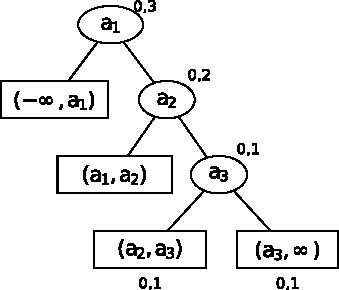
\includegraphics[width=.3\textwidth]{kap3OptimaleSB3}}

  \caption{Drei mögliche Suchbäume über die Elemente $S=\{a_1, a_2, a_3\}$ mit bekannter Zugriffswahrscheinlichkeit $0{,}1 - 0{,}3$.}
  \label{kap3OptimaleSB}
\end{figure}

Die erwartete durchschnittliche Suchzeit (Zahl der Vergleiche) für die in Abbildung \vref{kap3OptimaleSB} dargestellten Suchbäume ist:
\begin{align*}
  P_{T_1} &= (0{,}2 + 0{,}3 \cdot 2 + 0{,}1 \cdot 2) + (2 \cdot 0{,}1 + 2 \cdot 0{,}1 + 2 \cdot 0{,}1 + 2 \cdot 0{,}1)\\
          &= 1{,}8\\
  P_{T_2} &= (0{,}1 + 0{,}2 \cdot 2 + 0{,}3 \cdot 3) + (0{,}1 + 0{,}1 \cdot 2 + 0{,}1 \cdot 3 + 0{,}1 \cdot 3)\\
          &= 2{,}3\\
  P_{T_3} &= (0{,}3 + 0{,}2 \cdot 2 + 0{,}1 \cdot 3) + (0{,}1 + 0{,}1 \cdot 2 + 0{,}1 \cdot 3 + 0{,}1 \cdot 3)\\
          &= 1{,}9\\
\end{align*}

In diesem Beispiel, ist also der Baum $T_1$ besser, als die Bäume $T_2$ oder $T_3$.

\subsubsection{Optimale BST und dynamische Programmierung}
Per \textit{brute force} alle möglichen Suchbäume zu erzeugen und zu untersuchen, lässt sich jedoch nur für sehr kleine $|S|=n$ durchführen. Es gibt $\binom{2n}{n} \cdot \frac{1}{n+1} \approx 4^n$ mögliche Suchbäume, das heißt bereits bei $n=5$ wären über $1.000$ Bäume zu untersuchen. Mit der Methode des \textit{dynamischen Programmierens} können wir das Problem jedoch effizienter lösen. 

\textit{Dynamische Programmierung} bietet sich an, wenn sich ein Problem in kleinere Teilprobleme zerlegen lässt, die sich wiederum in kleinere Teilprobleme zerlegen lassen. Die kleinste Einheit dieser Teilprobleme wird gelöst, die Lösung gespeichert, so dass sie für die Lösung verschiedener größerer Teilprobleme genutzt werden kann, ohne jedes mal neu bestimmt zu werden. Jedes Teilproblem muss so nur einmal gelöst werden, auch wenn es zum Gesamtproblem mehrfach beiträgt.

Versuchen wir nun die Suche nach einem optimalen binären Suchbaum in solche Teilprobleme aufzuteilen:
\begin{itemize}
  \item Sei $S'=\{a_i, \ldots, a_j\}$ eine Teilmenge  der Menge $S$, also $S' \subset S$.
  \item Mit $T_{i,j}$ bezeichnen wir den optimalen Suchbaum für $S'$.
  \item Die Wurzel von $T_{i,j}$ sei $a_m$, $m \in \{i, \ldots, j\}$.
  \item Die inneren Knoten von $T_{i,j}$ sind $\{a_i, \ldots, a_j\}$.
  \item Wir speichern $(a_{i-1}, a_i), (a_i, a_{i+1}) \ldots, (a_{j-1}, a_j), (a_j, a_{j+1})$ in den Blättern von $T_{i,j}$, also genau wie bei $S$ die Intervalle über die Bereiche vor, zwischen und nach den gespeicherten Elementen.
  \item Mit $P_{T_{i,j}}$ bezeichnen wir die erwartete durchschnittliche Anzahl an Vergleichen, um zu bestimmen, ob ein Element im Teilbaum $T_{i,j}$ gespeichert ist, oder nicht, unter der Bedingung, dass wir die Suche bereits auf den Teilbaum eingeschränkt haben.
  \item Die Zugriffswahrscheinlichkeiten auf Elemente des Teilbaums (die in den inneren Knoten gespeichert werden) geben wir mit $\widetilde{p_i} = \frac{p_i}{w_{i,j}}$ an, die Zugriffswahrscheinlichkeiten auf seine Blätter mit $\widetilde{q_i} = \frac{q_i}{w_{i,j}}$ an. Dabei bezeichnet $w_{i,j}$ die Wahrscheinlichkeit, dass nach einem Element $a \in [a_i, a_j]$ gesucht wird, also $w_{i,j} = p_i + \ldots + p_j + q_{i-1} + q_i + \ldots + q_j$. $\widetilde{p_i}$ und $\widetilde{q_i}$ sind also bedingte Wahrscheinlichkeiten.\footnote{$P(A|B)=\frac{P(A \cap B)}{P(B)}$ und wenn $A \subset B$, dann $P(A|B) = \frac{P(A)}{P(B)}$.}
\end{itemize}

\begin{figure}[hbt]
  \centering
  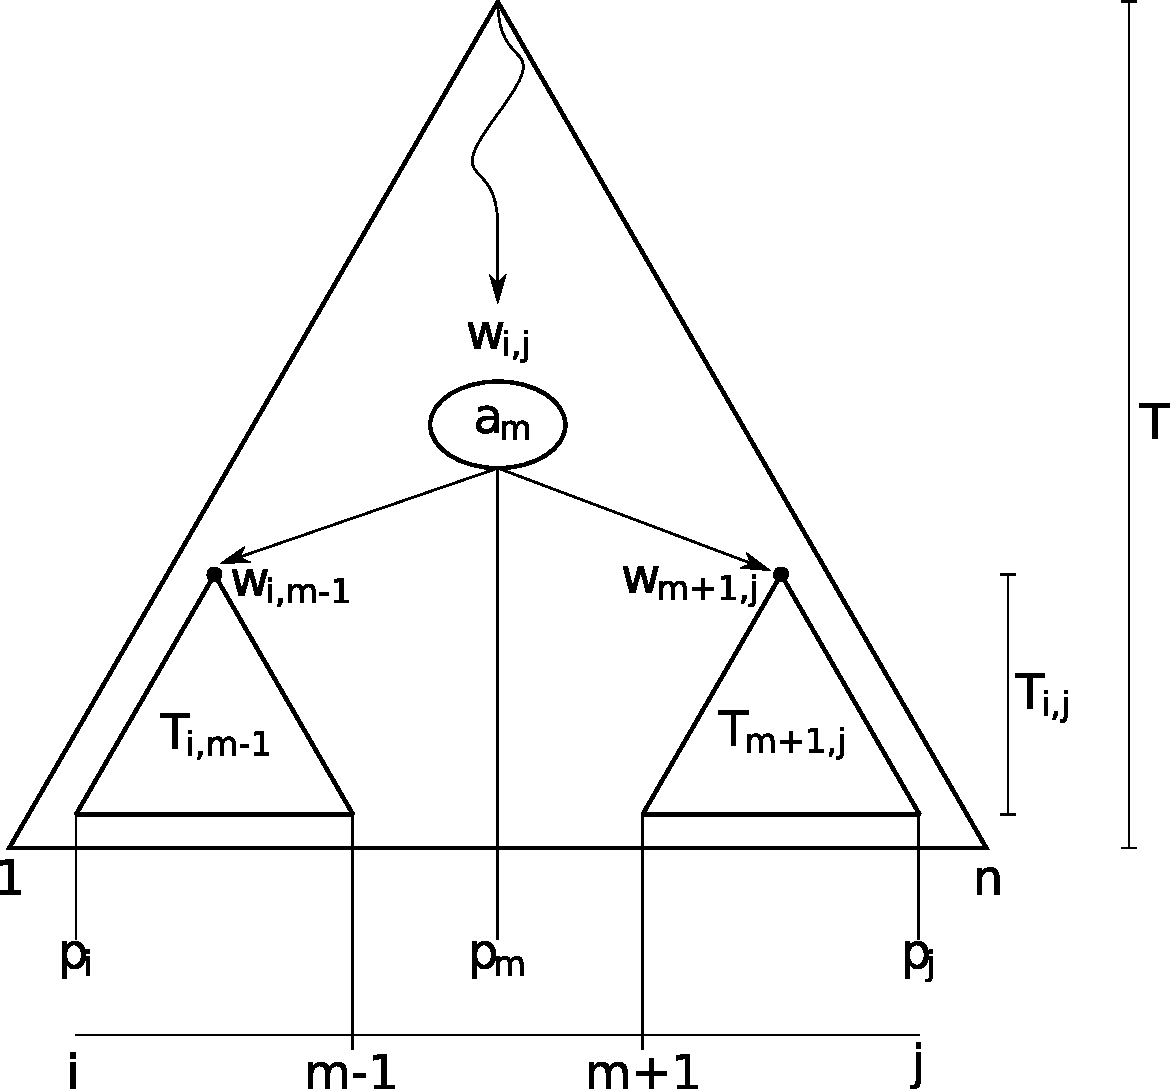
\includegraphics[width=.5\textwidth]{kap3SucheOSB}
  \caption{Die Suche eines optimalen Suchbaums lässt sich in Teilprobleme aufspalten. Darstellung zur Veranschaulichung der Bezeichnungen der Teilbäume und wichtiger Knoten.}
  \label{kap3SucheOSB}
\end{figure}

Wir wissen, dass sich $T_{i,j}$ aus $a_m$ und zwei Teilbäumen zusammensetzt: $T_{i, m-1}$ und $T_{m+1,j}$. Abbildung \ref{kap3SucheOSB} veranschaulicht das. Dies nutzen wir um die erwartetet Anzahl von Vergleichen in $T_{i,j}$ zu bestimmen. Zu beachten ist, dass $\widetilde{p_i}=\frac{p_i}{w_{i,j}}$ und $\widetilde{q_i}=\frac{q_i}{w_{i,j}}$ gilt.
\begin{align*}
P_{T_{i,j}} &= \sum_{k=i}^{j} \widetilde{p_k} \cdot (Tiefe(k) + 1) + \sum_{k=i-1}^{j} \widetilde{q_k} \cdot Tiefe'(k) \\
	&= \frac{1}{w_{i,j}} \cdot \left( \sum_{k=i}^{j} p_k \cdot (Tiefe(k) + 1) + \sum_{k=i-1}^{j} q_k \cdot Tiefe'(k) \right)\\
	&= \frac{1}{w_{i,j}} \cdot \left( \sum_{k=i}^{m-1} p_k \cdot (Tiefe(k) + 1) + p_m + \sum_{k=m+1}^{j} p_k \cdot (Tiefe(k) + 1)\right. \\
	& \phantom{= \frac{1}{w_{i,j}}} \quad \left. + \sum_{k=i-1}^{m-1} q_k \cdot Tiefe'(k) + \sum_{k=m}^{j} q_k \cdot Tiefe'(k)\right)
\end{align*}
Wenn wir hier die Summen durch die Formeln für die Teilbäume ersetzen müssen wir zwei Dinge berücksichtigen. $P_{T_{i,m-1}}$ berechnet die bedingte Wahrscheinlichkeit, bedingt darauf, dass wir nach einem Knoten in dem Teilbaum $T_{i,m-1}$ gefragt werden. Wir wissen bereits, dass wir in dem Teilbaum sind, müssen daher $P_{T_{i,m-1}}$ mit $w_{i,m-1}$ multiplizieren. Die Formel für $P_{T_{i,m-1}}$ berücksichtigt die Tiefe eines Knotens, bzw. die Tiefe eines Blattes. Von $P_{T_{i,m-1}}$ aus betrachtet ist die Tiefe jedoch um $1$ geringer, als von $P_{T_{i,j}}$ aus betrachtet.
\begin{align*}
  P_{T_{i,j}} &= \frac{1}{w_{i,j}} \cdot \left( \sum_{k=i}^{m-1} p_k \cdot (Tiefe(k) + 1) + \sum_{k=i-1}^{m-1} q_k \cdot Tiefe'(k) + p_m \right.\\
    & \phantom{= \frac{1}{w_{i,j}}} \quad \left. + \sum_{k=m+1}^{j} p_k \cdot (Tiefe(k) + 1) + \sum_{k=m}^{j} q_k \cdot Tiefe'(k) \right)\\
    &= \frac{ w_{i,m-1} \cdot P_{T_{i,m-1}} +  w_{i,m-1} + p_m + w_{m+1, j} + w_{m+1,j} \cdot P_{T_m+1, j} }{w_{i,j}}\\
    &= 1 + \frac{w_{i,m-1} \cdot P_{T_{i,m-1}} + w_{m+1, j} \cdot P_{T_{m+1,j}}}{w_{i,j}}
\end{align*}

%\[ P_{T_{i,j}} = \sum_{k=i}^{j} \widetilde{p_k} \cdot (Tiefe(k) + 1) + \sum_{k=i-1}^{j} \widetilde{q_k} \cdot Tiefe'(k) \]
%Wir lösen nun $\widetilde{p_k}$ und $\widetilde{q_k}$ auf, da $\widetilde{p_i}=\frac{p_i}{w_{i,j}}$ und $\widetilde{q_i}=\frac{q_i}{w_{i,j}}$.
%\[ P_{T_{i,j}} = \frac{1}{w_{i,j}} \cdot \left( \sum_{k=i}^{j} p_k \cdot (Tiefe(k) + 1) + \sum_{k=i-1}^{j} q_k \cdot Tiefe'(k) \right) \]
%Wir teilen die Summenformeln neu auf, wobei wir beachten, dass $Tiefe(m) = 0$, weil $a_m$ die Wurzel von $T_{i,j}$ ist.
%\[ \sum_{k=i}^{j} p_k \cdot (Tiefe(k) + 1) = \sum_{k=i}^{m-1} p_k \cdot (Tiefe(k) + 1) + p_m + \sum_{k=m+1}^{j} p_k \cdot (Tiefe(k) + 1) \]
%Analog gilt:
%\[ \sum_{k=i-1}^{j} q_k \cdot Tiefe'(k) = \sum_{k=i-1}^{m-1} q_k \cdot Tiefe'(k) + \sum_{k=m}^{j} q_k \cdot Tiefe'(k) \]
%Wir können nun die Formel für den Teilbaum $T_{i, m-1}$ aufstellen:
%\[ P_{T_{i,m-1}} = \sum_{k=i}^{m-1} \widehat{p_k} \cdot (Tiefe(k) + 1) + \sum_{k=i-1}^{m-1} \widehat{q_k} \cdot Tiefe'(k)\]
%wobei natürlich $\widehat{p_k} = \frac{p_k}{w_{i,m-1}}$ und $\widehat{q_k} = \frac{q_k}{w_{i,m-1}}$. Genauso lässt sich die Formel für den Teilbaum $T_{m+1,j}$ aufstellen:
%\[ P_{T_{m+1, }} = \sum_{k=m+1}^{j} \overline{p_k} \cdot (Tiefe(k) + 1) + \sum_{k=m}^{j} \overline{q_k} \cdot Tiefe'(k) \]
%natürlich mit $\overline{p_k} = \frac{p_k}{w_{m+1, j}}$ und $\overline{q_k} = \frac{q_k}{w_{m+1, j}}$. Wenn wir das zu einer Formel zusammenfassen, müssen wir beachten, dass wir nicht mehrfach berücksichtigen, die Suche bereits auf einen Teilbaum beschränkt zu haben. Wir müssen daher $P_{T_{i,m-1}}$ mit $w_{i,m-1}$ multiplizieren und $P_{T_{m+1,j}}$ mit $w_{m+1, j}$.
%
%Wir können das nun zu einer neuen Formel für $P_{T_{i,j}}$ zusammenfassen:
%\[ P_{T_{i,j}} = \frac{w_{i,m-1} \cdot P_{T_{i,m-1}} + p_m + w_{m+1, j} \cdot P_{T_{m+1,j}}}{w_{i,j}} \]

%\begin{align*}
%  P_{T_{i,j}} &= \sum_{k=i}^{j} \widetilde{p_k} \cdot (Tiefe(k) + 1) + \sum_{k=i-1}^{j} \widetilde{q_k} \cdot Tiefe'(k)\\
%    &= \sum_{k=i}^{j} \frac{p_k}{w_{i,j}} \cdot (Tiefe(k) + 1) + \sum_{k=i-1}^{j} \frac{q_k}{w_{i,j}} \cdot Tiefe'(k)\\
%  w_{i,j} \cdot P_{T_{i,j}} &= \sum_{k=i}^{j} p_k \cdot (Tiefe(k) + 1) + \sum_{k=i-1}^{j} q_k \cdot Tiefe'(k)\\
%    &= \sum_{k=i}^{j} \left[ p_k \cdot (Tiefe(k) + 1) + q_k \cdot Tiefe'(k) \right] + q_{i-1} \cdot Tiefe'(i-1) \\
%    &= \sum_{k=i}^{m-1} \left[ p_k \cdot (Tiefe(k) + 1) + q_k \cdot Tiefe'(k) \right] \\
%    &\qquad + p_m \cdot (\underbrace{Tiefe(m)}_{=0} +1 ) + q_m \cdot Tiefe'(m) \\
%    &\qquad + \sum_{k=m+1}^j \left[ p_k \cdot (Tiefe(k) + 1) + q_k \cdot Tiefe'(k) \right] \\
%    &\qquad + q_{i-1} \cdot Tiefe'(i-1)\\
%    &= \sum_{k=i}^{m-1} \left[ w_{i,m-1} \cdot \frac{p_k}{w_{i,m-1}} \cdot (Tiefe(k) + 1) +  w_{i,m-1} \cdot \frac{q_k}{w_{i,m-1}} \cdot Tiefe'(k) \right] \\
%        &\qquad + p_m + q_m \cdot Tiefe'(m) + q_{i-1} \cdot Tiefe'(i-1)\\
%        &\qquad + \sum_{k=m+1}^j \left[ w_{m+1,j} \cdot \frac{p_k}{w_{m+1,j}} \cdot (Tiefe(k) + 1) + w_{m+1,j} \cdot \frac{q_k}{w_{m+1,j}} \cdot Tiefe'(k) \right] \\
%    &=  w_{i,m-1} \cdot \sum_{k=i}^{m-1} \left[\widehat{p_k} \cdot (Tiefe(k) + 1) + \widehat{q_k} \cdot Tiefe'(k) \right] \\
%            &\qquad + p_m + q_m \cdot Tiefe'(m) + q_{i-1} \cdot Tiefe'(i-1)\\
%            &\qquad + w_{m+1,j} \sum_{k=m+1}^j \left[ \overline{p_k} \cdot (Tiefe(k) + 1) + \overline{q_k} \cdot Tiefe'(k) \right] \\
%    &=  w_{i,m-1} \cdot P_{T_{i, m-1}} - q_{i-1} \cdot Tiefe'(i-1) \\
%    &\qquad +  p_m + q_m \cdot Tiefe'(m)  + q_{i-1} \cdot Tiefe'(i-1) \\
%    &\qquad + w_{m+1,j} \cdot P_{T_{m+1, j}} - q_m \cdot (Tiefe'(m)) \\
%    &= w_{i,m-1} \cdot P_{T_{i, m-1}} + p_m + w_{m+1,j} \cdot P_{T_{m+1, j}}\\
%    P_{T_{i,j}} &= \frac{w_{i,m-1} \cdot P_{T_{i, m-1}} + p_m + w_{m+1,j} \cdot P_{T_{m+1, j}}}{w_{i,j}}\\
%                &= 1 + \frac{w_{i,m-1} \cdot P_{T_{i, m-1}} + w_{m+1,j} \cdot P_{T_{m+1, j}}}{w_{i,j}}
%\end{align*}
%
%Daraus folgt:
%\[ P_{T_{i,j}} = 1 + \frac{w_{i,m-1} \cdot P_{T_{i,m-1}} + w_{m+1, j} \cdot P_{T_{m+1,j}}}{w_{i,j}} \]

\begin{Lma}
  \hspace{\parindent}Der Teilbaum $T_{i,j}$ sei ein optimaler binärer Suchbaum für die Menge $\{a_i, \ldots, a_j\}$. $a_m$ sei die Wurzel von $T_{i,j}$, $T_{i,m-1}$ der linke und $T_{m+1,j}$ der rechte Teilbaum von $T_{i,j}$. Dann ist $T_{i,m-1}$ der optimale binäre Suchbaum für die Menge $\{a_i, \ldots, a_{m-1}\}$ und $T_{m+1,j}$ der optimale binäre Suchbaum der Menge $\{a_{m+1}, \ldots, a_j\}$.
\end{Lma}

\begin{Bew}
  \hspace{\parindent}Angenommen es existiert ein Baum $T'_{i,m-1}$ mit $P_{T'_{i,m-1}} < P_{T_{i,m-1}}$. Dann wäre auch $P_{T'_{i,j}} < P_{T_{i,j}}$, da:
  \begin{align*}
    P_{T'_{i,j}} &= 1 + \frac{w_{i,m-1} \cdot P_{T'_{i,m-1}} + w_{m+1, j} \cdot P_{T_{m+1,j}}}{w_{i,j}}\\
      &< 1 + \frac{w_{i,m-1} \cdot P_{T_{i,m-1}} + w_{m+1, j} \cdot P_{T_{m+1,j}}}{w_{i,j}} = P_{T_{i,j}}
  \end{align*}
  dies steht aber in Widerspruch dazu, dass $P_{T_{i,j}}$ ein optimaler binärer Suchbaum ist. Jeder Teilbaum von $P_{T_{i,j}}$ muss daher selber ein optimaler binärer Suchbaum sein.
\end{Bew}

Wir haben nun alles zusammen um mit Hilfe der Methode des dynamischen Programmierens einen Algorithmus zum Finden eines optimalen binären Suchbaums anzugeben.
Wir vereinbaren folgende Variablen für den Algorithmus:
\begin{align*}
  r_{i,j} &:= \text{Index der Wurzel von } T_{i,j}\\
  c_{i,j} &:= w_{i,j} \cdot P_{T_{i,j}} = \text{ Kosten von } T_{i,j}\\
  w_{i,j} &:= \text{Wahrscheinlichkeit, dass } a \in \{a_i, \ldots, a_j\}
\end{align*}

Es ist leicht zu erkennen, dass $w_{i,j} = w_{i, m-1} + p_m + w_{m+1, j}$ gilt. Man kann $c_{i,j}$ auch rekursiv berechnen. $c_{i,j}$ setzt sich aus den Kosten seiner Teilbäume zusammen, die Tiefe der Knoten in den Teilbäumen ist jedoch um eins erhöht. Daher gilt: $c_{i,j} = c_{i,m-1} + p_m + c_{m+1,j} + w_{i,m-1} + w_{m+1,j} = w_{i,j} + c_{i,m-1} + c_{m+1, j}$. Für $i=m$ gibt es keinen linken Teilbaum, für $m=j$ gibt es keinen rechten Teilbaum. $T_{i,i}$ definieren wir als leeren Baum, mit dem Gewicht $w_{i,i} = q_i$ und den Kosten $c_{i,i}=0$.

% Algorithmus aus dem Vorlesungsskript
\begin{Alg}[Finden eines optimalen binären Suchbaums]
\begin{algorithmic}[1]
  \Function{Finde Baum}{$p_1, \ldots, p_n$, $q_0, \ldots, q_n$}
    \For{$i = 0, \ldots, n$}
      \State $w_{i+1,i} = q_i$
      \State $c_{i+1,i} = 0$
    \EndFor
    \For{$k=0, \ldots, n-1$}
      \For{$i=1, \ldots, n-k$}
        \State $j=i+k$
        \State Bestimme $m$ mit $i \le m \le j$, so dass $c_{i,m-1} + c_{m+1,j}$ minimal ist.
        \State $r_{i,j} = m$
        \State $w_{i,j} = w_{i,m-1} + p_m + w_{m+1, j}$
        \State $c_{i,j} = c_{i, m-1} + c_{m+1, j} + w_{i, j}$
      \EndFor
    \EndFor
  \EndFunction
\end{algorithmic}
\end{Alg}

% Aho, Hopcroft, Ullman: The Design an Analysis of Computer Algorithms
%\begin{Alg}[Finden eines optimalen binären Suchbaums]
%\begin{algorithmic}[1]
%  \For{$i = 0, \ldots, n$}
%    \State $w_{i,i} = q_i$
%    \State $c_{i,i} = 0$
%  \EndFor
%  \For{$k=1, \ldots n$}
%    \For{$i=0, \ldots, n-k$}
%      \State $j=i+k$
%      \State Bestimme $m$ mit $i < m \le j$, so dass $c_{i,m-1} + c_{m+1,j}$ minimal ist.
%      \State $r_{i,j} = m$
%      \State $w_{i,j} = w_{i,m-1} + p_m + w_{m+1, j}$
%      \State $c_{i,j} = c_{i, m-1} + c_{m+1, j} + w_{i, j}$
%    \EndFor
%  \EndFor
%\end{algorithmic}
%\end{Alg}

Der Algorithmus basiert auf einem von Richard Bellman 1957 gefundenen Satz über optimale mittlere Suchdauer in binären Suchbäumen. Die Teilprobleme, in die die Suche nach dem optimalen binären Suchbaum aufgeteilt wird, sind die Teilbäume $T_i,j$. Der Algorithmus sucht für jeden dieser Teilbäume die optimale Wurzel, bestimmt das Gewicht des Teilbaums und die Kosten für die Suche im Teilbaum. Diese Werte werden dann genutzt, um größere Teilbäume zu berechnen. Als Ergebnis bekommen wir die Wurzeln aller Teilbäume, angefangen bei Teilbäumen, die lediglich einen Knoten enthalten, bis zum gesuchten Teilbaum $T_{1,n}$.

\subsubsection{Beispielhafte Suche nach dem optimalen binären Suchbaum}
Wer veranschaulichen das Vorgehen des Algorithmus, in dem wir das Beispiel von oben nachvollziehen. $S$ ist demnach die Menge $\{2, 5, 6\}$ mit den Zugriffswahrscheinlichkeiten $p_1 = 0{,}3,\quad p_2 = 0{,}2,\quad p_3 = 0{,} 1$ und $q_0 = q_1 = q_2 = q_3 = 0{,}1$. Der Algorithmus erzeugt dann folgende Tabelle:

\begin{center}
\begin{tabular}{|>{$}c<{$}||>{$}c<{$}|>{$}c<{$}|>{$}c<{$}|>{$}c<{$}|>{$}c<{$}|}\hline
 & i=0 & i=1 & i=2 & i=3 \\\hline\hline
\multirow{2}*{Init} & w_{1,0}=0{,}1 & w_{2,1} = 0{,}1 & w_{3,2}= 0{,}1 & w_{4,3} = 0{,}1 \\
                    & c_{1,0}=0\hphantom{0} & c_{2,1} = 0\hphantom{0} & c_{3,2}=0\hphantom{0} & c_{4,3}=0\hphantom{0}\\\hline
\multirow{3}*{k=0}  & & r_{1,1}=1\hphantom{0} & r_{2,2}=2\hphantom{0} & r_{3,3}=3\hphantom{0} \\
                    & & w_{1,1}=0{,}5 & w_{2,2}=0{,}4 & w_{3,3}=0{,}3\\
                    & & c_{1,1}=0{,}5 & c_{2,2}=0{,}4 & c_{3,3}=0{,}3\\\hline
\multirow{3}*{k=1}  & & r_{1,2}=1\hphantom{0}& r_{2,3}=2\hphantom{0}& \\
                    & & w_{1,2}=0{,}8 & w_{2,3}=0{,}6 & \\
                    & & c_{1,2}=1{,}2 & c_{2,3}=0{,}9 & \\\hline
\multirow{3}*{k=2}  & & r_{1,3}=2\hphantom{0}& & \\
                    & & w_{1,3}=1{,}0 & & \\
                    & & c_{1,3}=1{,}8 & & \\\hline
\end{tabular}
\end{center}

Aus dieser Tabelle lässt sich nun leicht der optimale binäre Suchbaum erstellen.
\begin{Alg}
\begin{algorithmic}[1]
  \Procedure{Erzeuge Baum}{$i$, $j$}
    \State Erzeuge Knoten $v_{i,j}$ als Wurzel von $T_{i,j}$.
    \State Knoten $v_{i,j}$ wird dabei mit $s_{r_{i,j}}, \text{ mit } s \in S$ beschriftet.
    \If{$i < r_{i,j}$}
      \State \textsc{Erzeuge Baum}($i$, $r_{i,j}-1$) als linken Teilbaum von $v_{i,j}$
    \EndIf
    \If{$r_{i,j} < j$}
      \State \textsc{Erzeuge Baum}($r_{i,j} + 1$, $j$) als rechten Teilbaum von $v_{i,j}$
    \EndIf
  \EndProcedure
\end{algorithmic}
\end{Alg}

Wir beginnen  mit \textsc{Erzeuge Baum($1, 3$)}. Die Wurzel $v_{1,3}$ ist $a_2$. Um den linken Teilbaum zu erzeugen rufen wir \textsc{Erzeuge Baum($1, 1$)} auf und finden $v_{1,1} = a_1$. Um den rechten Teilbaum zu erzeugen rufen wir \textsc{Erzeuge Baum($3, 3$)} auf und finden die Wurzel $v_{3,3} = a_2$. Anschließend erzeugen wir die Blätter, per Definition als Intervalle. Wir erhalten so den Baum, den wir bereits in Abbildung \vref{kap3OptimaleSBT1} gesehen haben.

\subsubsection{Analyse von Laufzeit und Speicherverhalten}
Der Algorithmus muss die Zwischenergebnisse speichern. Eine Tabelle, wie wir sie oben genutzt haben können wir als Matrix $M \in \mathcal{M}((n + 1) \times n, \mathbb{R})$ auffassen. Der Speicherplatz beträgt also $S(n) = n \cdot (n+1) = n^2 + n \in \mathcal{O}(n^2)$.

Betrachten wir das Laufzeitverhalten des Algorithmus. Die Zeilen 2 bis 5 können wir mit $c_1 \cdot (n+1)$ ansetzen. Zeile 8 ist eine einfache Operation konstanter Zeit, im folgenden mit $c_2$ berücksichtigt. In Zeile 9 müssen wir $(j-i) = k$ zuvor berechnete Werte nachschauen und vergleichen. Dafür berechnen wir $k \cdot c_3$. Zeile 10 bis 12 brauchen wieder konstante Zeit, also $c_4$. Daher:
\[ T(n) = c_1 \cdot n + c_1 + \sum_{k=0}^{n-1} \sum_{i=1}^{n-k} \left( c_2 + k \cdot c_3 + c_4\right) \]
$c_2 + c_4$ fassen wir zu $c_5$ zusammen:
\begin{align*}
  T(n) &= c_1 \cdot n + c_1 + \sum_{k=0}^{n-1} \sum_{i=1}^{n-k} \left( c_5 + k \cdot c_3 \right)\\
       &= c_1 \cdot n + c_1 + \sum_{k=0}^{n-1} \left( (n-k) \cdot c_5 + (n-k) \cdot k \cdot c_3 \right)\\
       &= c_1 \cdot n + c_1 + c_5 \cdot \sum_{k=0}^{n-1} (n-k) + c_3 \cdot \sum_{k=0}^{n-1} (nk - k^2)\\
       &= c_1 \cdot n + c_1 + c_5 \cdot \sum_{k=1}^{n} k + c_3 \cdot \left( n \cdot \sum_{k=1}^{n-1} k - \sum_{k=1}^{n-1} k^2\right)\\
       &= c_1 \cdot n + c_1 + c_5 \cdot \frac{n^2 + n}{2} + c_3 \cdot \left( n \cdot \left( \frac{n^2 + n}{2} -n \right) - \frac{2n^3 + 3n^2 + n}{6} -n^2 \right)\\
       &= c_1 \cdot n + c_1 + c_5 \cdot \frac{n^2 + n}{2} + c_3 \cdot \left( \frac{n^3 - n}{6} \right)\\
       &\in \mathcal{O}(n) + \mathcal{O}(n^2) + \mathcal{O}(n^3)
\end{align*}
Der Algorithmus liegt also in $\mathcal{O}(n^3)$.

\subsubsection{Optimierung}
Durch die dynamische Programmierung hat der Algorithmus mindestens quadratische Laufzeit. Die kubische Laufzeit des Algorithmus beruht auf einer Kombination des dynamischen Programmierens und der Suche nach der Wurzel in Zeile 9 des Algorithmus. Donald E. Knuth hat in seinem Buch \textit{The Art of Computer Programming} Band 3: \textit{Sorting and Searching.} folgendes Lemma bewiesen:

\begin{Lma}
  \hspace{\parindent}$r_{i,j-1} \le r_{i,j} \le r_{i+1, j}$.
\end{Lma}

Durch die Eingrenzung der Wurzelsuche durch das Lemma, kann die Laufzeit des Algorithmus auf $T(n) \in \mathcal{O}(n^2)$ reduziert werden.

% vorlesung 10
\subsection{Sonstige Datenstrukturen für das Wörterbuchproblem}
Binäre Suchbäume weißen in schlechten Fällen, schlechte Laufzeiten bei der Suche auf. Als Antwort darauf haben wir uns balancierte Bäume angeschaut, z.B. AVL-Bäume oder $(a,b)$-Bäume, die oft als B-Bäume bezeichnet werden. Es gibt noch mehr Bäume mit verschiedenen Vorschriften. Wir haben uns schließlich optimale binäre Suchbäume angeschaut. Oft kennt man die Wahrscheinlichkeiten nicht, wie oft man nach welchen Daten gefragt wird, kann also keinen optimalen Suchbaum aufbauen.

Es gibt weitere Datenstrukturen für das Wörterbuchproblem. Einige arbeiten zum Beispiel mit einer Move"=To"=Front"=Heuristik. Dabei werden die Daten, nach denen gefragt wird, so verschoben, dass sie schneller zu finden sind, als Daten, nach denen lange nicht mehr gefragt wurden (z.B. an den Anfang einer Liste oder eines Arrays). Ein solche Vorgehen lässt sich auch auf Bäumen implementieren: Splay-Trees sind selbstorganisierende Suchbäume. Die Daten, auf die zugegriffen wird, werden durch Rotation und Doppelrotation innerhalb des Baums "`nach oben"' bewegt.

Für spezielle Datenmengen lassen sich noch bessere Datenstrukturen entwickeln. Ein \textit{Trie} ist ein digitaler Suchbaum, der zum Beispiel gerne von Suchmaschinen im Internet, von Programmen zur Textverarbeitung oder in der Bioinformatik zur Speicherung von DNA"=Folgen genutzt wird.

\begin{figure}[hbt]
  \centering
  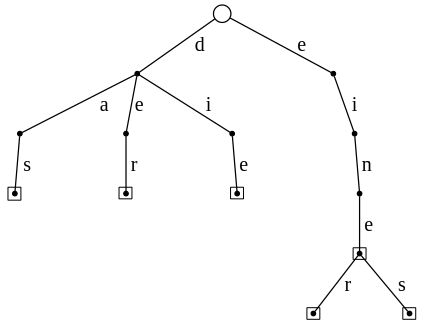
\includegraphics[scale=.5]{kap3Trie}
  \caption{Ein Trie, der die bestimmten und unbestimmten Artikel enthält.}
  \label{trie}
\end{figure}

In Abbildung \vref{trie} sehen wir ein einfaches Beispiel eines Tries. Das lässt sich zu Gunsten der Effizienz noch vereinfachen. Suffixbäume zum Beispiel sind Tries, die alle Suffixe eines Wortes speichern. Zur Konstruktion und Darstellung braucht man lineare Zeit im Verhältnis zur Wortlänge. Suffixbäume sind für DNA besonders gut geeignet. Suffixarrays vereinfachen diesen Ansatz noch.

\section{Prioritätswarteschlangen (priority queues)}
Eine weitere wichtige Datenstruktur, die wir im Folgenden immer wieder nutzen werden sind Prioritätswarteschlangen. Die üblichen Operationen auf einer Prioritätswarteschlange sind:
\begin{itemize}
  \item Streichen des Minimums (\texttt{delete-min}): finde und streiche das kleinste Objekt, also das Objekt mit der höchsten Priorität.
  \item Einfügen eines neuen Objekts (\texttt{insert}): hinzufügen eines neuen Objekts in die Warteschlange.
  \item Vermindere einen Schlüssel (\texttt{decrease-key}): vermindere den Wert eines Schlüssels, erhöhe also die Priorität eines Objekts.
\end{itemize}

Die Standarddatenstruktur dafür ist ein (binärer) Heap. Betrachten wir daher kurz die Laufzeiten der oben genannten Operationen auf einem einfachen und einem Fibonacci"=Heap:

\begin{center}
\begin{tabular}{lcc}
& Heap & \multirow{2}*{Fibonacci-Heaps}\\
& (schlechtester Fall) & \\\hline\hline
Streiche Minimum & $\Theta(\log n)$ & $\Theta(1)$ (amortisiert)\\
Einfügen & $\Theta(\log n)$ & $\mathcal{O}(\log n)$ (schlechtester Fall)\\
Vermindere Schlüssel & $\Theta(\log n)$ & $\Theta(1)$ (amortisiert)\\\hline\hline
\end{tabular}\\
\end{center}

$\mathcal{O}(\log n)$ Zeit ist auch mit Standarddatenstrukturen für Wörterbücher möglich, mit einem Heap jedoch einfacher zu implementieren.

\section{Union-Find (disjoint sets)}
Union-Find bezeichnet sowohl ein Problem, als auch eine Datenstruktur. Gegeben ist eine feste Menge $S$ von Daten (o.B.d.A. $S = \{1, \ldots, n\}$). Gesucht ist eine Partition von $S$ in disjunkte Teilmengen, also $S = S_1 \cupdot S_2 \cupdot \ldots \cupdot S_k$. Darauf aufbauend definieren wir zwei Operationen:
\begin{itemize}
  \item \texttt{Union}($S_i$, $S_j$): vereinige zwei Teilmengen in der Partition und erzeuge so eine neue Partition.
  \item \texttt{Find}($i$): finde die Teilmenge der Partition, die $i$ enthält.
\end{itemize}

Hierfür gibt es eine Reihe von Anwendungen, von denen wir einige beispielhaft benennen wollen, ehe wir die Datenstruktur genauer untersuchen:
\begin{itemize}
  \item Finden der Zusammenhangkomponente eines Graphen, insbesondere: finden minimaler Spannbäume.
  \item Segmentierung von Bildern in der Bildverarbeitung: Erkennen und Zerlegen des Bildes in Segmente, die zusammen gehören (z.B. weil sie die gleiche Farbe haben).
  \item Equivalence(X, Y) in Fortran: Prüfen, ob X und Y verschiedene Bezeichner für das Gleiche sind. Man schafft dabei auf der Menge aller Variablen eines Programms eine Partition.
\end{itemize}

\begin{figure}[htb]
  \centering
  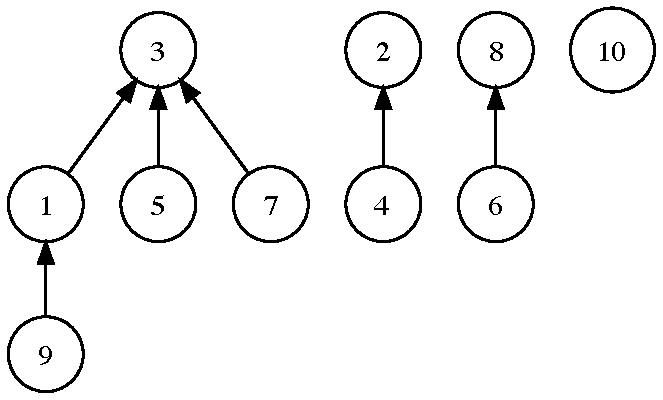
\includegraphics[scale=.66]{kap3UnionFind1}
  \caption{Beispiel einer Union"=Find"=Struktur mit $S= \{1, \ldots, 10 \}$ und den Partitionen $\{1, 3, 5, 7, 9\}$ $\{2, 4\}$ $\{6, 8\}$ $\{10\}$.}
  \label{kap3UnionFind1}
\end{figure}

Welche Datenstruktur wählen wir, um das Union"=Find"=Problem effizient zu lösen? Die Datenstruktur ist ein Wald, das heißt eine Menge von Bäumen. Wir brauchen einen Baum pro Teilmenge $S_1, \ldots, S_k$. Jede davon hat einen Repräsentanten $a \in S_i$, der sich in der Wurzel des entsprechenden Baums befindet. Die Verweise innerhalb eines Baums verlaufen vom Kind zum Vater.

Die Operationen lassen sich auf dieser Datenstruktur nun leicht konkretisieren. \texttt{Find}($x$) sucht den Knoten $x$ und folgt dem Pfad aufwärts bis zur Wurzel. Der Repräsentant, der in der Wurzel steht wird als Ergebnis der Operation zurück gegeben. \texttt{Union}($S_i, S_j$) macht die Wurzel des Baums von $S_j$ zu einem Kind der Wurzel von $S_i$. Die Laufzeit für \texttt{Union} liegt natürlich in $\mathcal{O}(1)$ . Die Laufzeit von \texttt{Find} ist abhängig von der Höhe des Baumes $h$: $\mathcal{O}(h)$. Die Abbildung \vref{kap3UnionFindOp} veranschaulicht beide Operationen.

\begin{figure}[htb]
  \centering
  \subfloat[\label{kap3UnionFindOp1}]{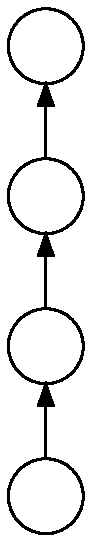
\includegraphics[scale=0.5]{kap3UnionFindOp1}}\hspace{3em}
  \subfloat[\label{kap3UnionFindOp2}]{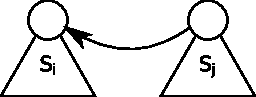
\includegraphics{kap3UnionFindOp2}}
  \caption{\subref{kap3UnionFindOp1} zeigt schematisch eine \texttt{Find}-Operation, Abbildung \subref{kap3UnionFindOp2} eine \texttt{Union}"=Operation.}
  \label{kap3UnionFindOp}
\end{figure}

Hat ein Baum die in Abbildung \vref{kap3UnionFindOp1} gezeigte Form, so hat \texttt{Find} eine Laufzeit von $\Theta(n)$. Dies lässt sich vermeiden, in dem die \texttt{Union}"=Operation immer den niedrigeren Baum an den Höheren hängt. Angenommen wir beginnen mit der Partition $\{1\}, \{2\}, \ldots, \{n\}$, und führen alle \texttt{Union}"=Operationen unter Beachtung des Höhenausgleichs durch, dann kann kein Baum die in Abbildung \vref{kap3UnionFindOp1} gezeigte Form annehmen.

\begin{Satz}
\hspace{\parindent}Führt man, beginnend mit der Partition $\{1\}, \ldots, \{n\}$, eine Folge von \texttt{Union}"=\texttt{Find}"=Operationen durch, wobei \texttt{Union} mit Höhenausgleich ausgeführt wird, so kostet \texttt{Union} $\mathcal{O}(1)$ und \texttt{Find} $\mathcal{O}(\log n)$ Zeit im schlechtesten Fall.
\end{Satz}

\begin{Bew}
\hspace{\parindent}Es ist zu zeigen, dass die Bäume nie höher werden als $\mathcal{O}(\log n)$. Dazu speichern wir mit jeder Wurzel noch die Höhe des Baums und zeigen durch Induktion über die Höhe $h$ eines Baums, dass jeder Baum $k \ge 2^h$ Knoten enthält.

Wir wählen als Induktionsanfang $h=0$. $2^h = 2^0 = 1$. Da ein Baum mit Höhe $0$ einen Knoten hat, stimmt die Induktionsvoraussetzung.

\begin{figure}[hbt]
  \centering
  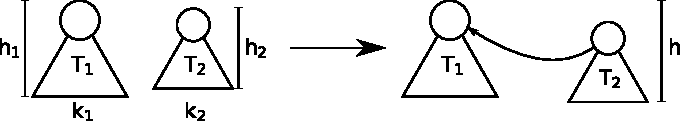
\includegraphics[width=0.9\textwidth]{kap3UnionFindLfzBew}
  \caption{Eine \texttt{Union}"=Operation mit Höhenausgleich, bei der ein Baum mit $k=k_1 + k_2$ Knoten und Höhe $h= max(h_1, h_2 +1)$ entsteht.}
  \label{kap3UnionFindLfzBew}
\end{figure}

Es folgt der Induktionsschritt $h-1 \to h$: in Abbildung \vref{kap3UnionFindLfzBew} sehen wir die \texttt{Union}"=Operation, aus der der Baum $T$ der Höhe $h=max(h_1, h_2 +1)$ mit $k=k_1+k_2$ Knoten entstanden ist. Angenommen $h_1 > h_2$: offensichtlich gilt $k_1 + k_2 \ge k_1$ und nach Induktionsvoraussetzung $k_1 \ge 2^{h_1} = 2^h$, daher auch $k \ge 2^h$. Falls aber $h_1 = h_2$ ist, so gilt $k_1 + k_2 \ge 2^{h_1} + 2^{h_2} = 2 \cdot 2^{h_2} = 2^{h_2 +1} = 2^{h}$.
\end{Bew}

Geht es noch besser? Bereits den Höhenausgleich kann man als eine Art Heuristik ansehen. Die \textit{Pfadkompression} geht davon aus, dass man Knoten oft in den gleichen Teilbäumen sucht. Sucht man z.B. nach einem Knoten a, so sammelt die Pfadkompression alle Knoten und Teilbäume, die auf dem Weg von der Wurzel zum Knoten a liegen und hängt diese gesammelten Knoten und Teilbäume direkt an die Wurzel an. Ein nachfolgender Zugriff auf einen der Knoten aus diesem Teilbaum wird deutlich schneller erfolgen. Abbildung \vref{kap3Pfadkompression} veranschaulicht das vorgehen.

\begin{figure}[htb]
  \centering
  \includegraphics[scale=.5]{kap3Pfadkompression}
  \caption{Pfadkompression: alle Knoten auf dem Weg von der Wurzel zu Knoten a werden direkt an die Wurzel gehängt.}
  \label{kap3Pfadkompression}
\end{figure}

%Was kostet \texttt{Union}-\texttt{Find} mit Höhenausgleich und Pfadkompression?
%Im schlechtesten Fall: immer noch $\mathcal{O}(1)$ beziehungsweise $\mathcal{O}(\log n)$.
%Amortisiert, ausgehend von $1 \ldots n$, dann Folge von \texttt{Union}s und \texttt{Find}s $\rightarrow$ res. Wald.
%
%definieren Rang eines Konten $v$: ursprünglich $0$, wird um $1$ erhöht, bei allen \texttt{Union}-Operationen wo $v$ Wurzel wird und zwei Wurzeln mit gleichen Rängen vorliegen.
%Zeichnung 7
%Heuristik: \texttt{Union} gemäß Rang: Baum, dessen Wurzel den kleineren Rang hat, wird an den gehängt, dessen Wurzel den größeren Rang hat.

% vorlesung 11

%Pfadkompression: man durchläuft einen Weg vom Knoten zur Wurzel. Dabei sammelt man alle Teilbäume auf dem Weg auf und hängt sie an die Wurzel. Dadurch sollte die nächste \texttt{Find}-Operation schneller ablaufen.

\subsection{Amortisierte Laufzeitanalyse von Union"=Find mit Pfadkompression}
Die Analyse der Laufzeit von Union"=Find mit Pfadkompression wird eine der komplizierteren in dieser Vorlesung.

Wir nehmen an, dass am Anfang jedes Elemente aus $S$ eine einelementige Menge bildet. Dann wird eine Folge $\sigma$ von \texttt{Union"=Find}"=Operationen ausgeführt. \texttt{Union} arbeitet dabei gemäß des Rangs der Wurzelknoten, der beiden zu vereinigenden Bäume. Zu jedem Knoten wird dazu sein Rang gespeichert. Am Anfang haben alle Knoten Rang $0$, falls zwei Bäume vereinigt werden, deren Wurzeln den gleichen Rang $r$ haben, so erhält die neue Wurzel den Rang $r+1$.

\begin{figure}[htb]
  \centering
  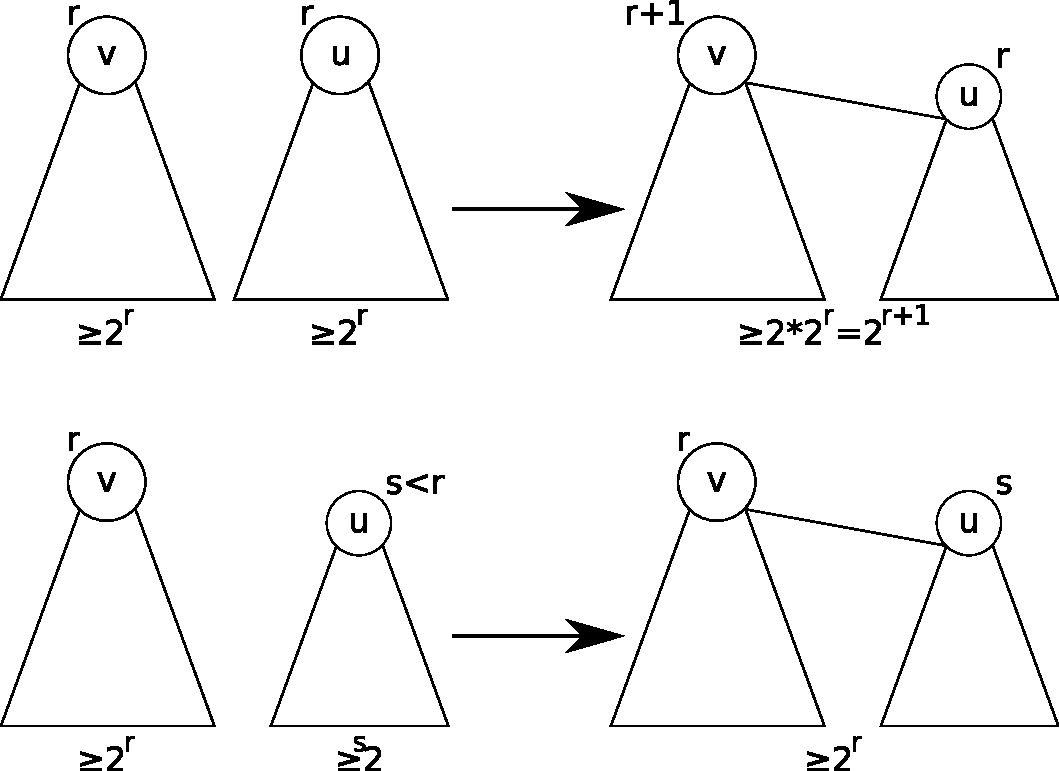
\includegraphics[width=.75\textwidth]{kap3UnionByRang}
  \caption{Der Rang eines Wurzelknotens erhöht sich, wenn zwei Bäume vereinigt werden, deren Wurzelknoten gleichen Rang haben. Haben die Wurzelknoten unterschiedlichen Rang, ändern sich die Ränge nicht und der Wurzelknoten mit kleinerem Rang wird an den Wurzelknoten mit höherem Rang angefügt.}
  \label{kap3UnionByRang}
\end{figure}

In Abbildung \vref{kap3UnionByRang} sehen wir, wie Union nach Rang funktioniert und wie es sich auf den Rang eines Knotens auswirkt. Wir können nun einige Eigenschaften festhalten. Für alle Knoten $v$, Wurzel eines Unterbaums $T_v$ gilt:
\begin{enumerate}
  \item $T_v$ hat mindestens $2^{Rang(v)}$ Knoten.
  \item es gibt $\le \frac{n}{2^r}$ Knoten vom Rang $r$ (folgt direkt aus 1.)
  \item alle Ränge sind $\le \log n$ (folgt direkt aus 2.)
  \item Falls bei der Ausführung von $\sigma$ irgendwann $w$ Nachkomme von $v$ ist, dann ist der $Rang(w) < Rang(v)$. Denn jede Kante ist durch eine \texttt{Union}"=Operation entstanden, nach der $Rang(w) < Rang(v)$ (siehe Abbildung \vref{kap3UnionByRang}). \texttt{Find}"=Operationen ändern daran nichts.
\end{enumerate}

\begin{Bem}
  \hspace{\parindent}Für alle Knoten $v$, Wurzel eines Unterbaums $T_v$ gilt: Höhe $T_v \le Rang(v)$. Die Pfadkompression ändert daran nichts, da bei Pfadkompression zwar die Höhe geringer wird, der Rang sich jedoch nicht verändert.

  Auch für Union nach Rang ist der schlechteste Fall für \texttt{Find} $\mathcal{O}(\log n)$.
\end{Bem}

Zur amortisierten Analyse von Union"=Find mit Pfadkompression brauchen wir eine sehr schnell und eine sehr langsam wachsende Funktion. Wir definieren die Funktionen $F,G : \mathbb{N} \to \mathbb{N}$ wie folgt:

\begin{align*}
  F(0) &= 1 \\
  F(i) &= 2^{F(i-1)} \quad i=1, 2, 3, \ldots
\end{align*}

Bereits die ersten Werte der Funktion lassen ihr sehr starkes Wachstum erkennen.
\begin{center}
  \begin{tabular}{>{$}l<{$}|>{$}r<{$}|>{$}r<{$}|>{$}r<{$}|>{$}r<{$}|>{$}r<{$}|>{$}r<{$}|>{$}r<{$}}
    i & 0 & 1 & 2 & 3 & 4 & 5 & 6 \\\hline
    F(i) & 1 & 2 & 4 & 16 & 65536 & 2^{65536} & 2^{2^{65536}}
  \end{tabular}
\end{center}

Die Funktion $G$ ist eine sehr langsam wachsende Funktion. Wir definieren sie mit Bezug auf $F(n)$:
\[G(n) = min\{k \mid F(k) \ge n \}\]

Auch hier wollen wir exemplarisch einige Werte betrachten:
\begin{center}
  \begin{tabular}{>{$}l<{$}|>{$}r<{$}|>{$}r<{$}|>{$}r<{$}|>{$}r<{$}|>{$}r<{$}|>{$}r<{$}|>{$}r<{$}|>{$}r<{$}|>{$}r<{$}|>{$}r<{$}|>{$}r<{$}|>{$}r<{$}|>{$}r<{$}}
    n    & 0 & 1 & 2 & 3 & 4 & 5 & 6 & \ldots & 16 & \ldots & 65536 & \ldots & 2^{65536} -1 \\\hline
    G(n) & 0 & 0 & 1 & 2 & 2 & 3 & 3 & 3 & 3 & 4 & 4 & 5 & 5
  \end{tabular}
\end{center}

$G(n)$ heißt auch $\log^* n$ : wie oft muss man den Logarithmus auf $n$ anwenden damit man auf eine Zahl $\le 1$ kommt?

Wir hatten bereits angenommen, dass jedes Element aus $S$ am Anfang eine einelementige Menge bildet und dann eine Folge $\sigma$ von \texttt{Union"=Find}"=Operationen ausgeführt wird. Gehen wir weiter davon aus, dass $\sigma$ aus $\le n-1$ \texttt{Union}- und $m$ \texttt{Find}"=Operationen besteht. Wir teilen die Ränge der Knoten in Gruppen auf:

\begin{center}
  \begin{tabular}{l|>{$}r<{$}|>{$}r<{$}|>{$}r<{$}|>{$}r<{$}|>{$}r<{$}|>{$}r<{$}|>{$}r<{$}|>{$}r<{$}|>{$}r<{$}}
    $r$           & 0 & 1 & 2 & 3 & 4 & 5 & \ldots & 16 & \ldots\\\hline
    Gruppe $G(r)$ & 0 & 0 & 1 & 2 & 2 & 3 &      3 & 3 & \ldots
  \end{tabular}
\end{center}

Jedes \texttt{Union} kostet $\mathcal{O}(1)$ Zeit. \texttt{Find} kostet mehr, proportional zur Länge des Weges bis zur Wurzel. Im folgenden führen wir eine amortisierte Analyse mittels Buchhalter Methode durch. Für jeden Knoten $v$ auf dem Weg zur Wurzel entstehen konstante Kosten in Höhe von 1 \euro{}. Diese ordnen wir
\begin{enumerate}
  \item der \texttt{Find}"=Operation zu, falls $v$ die Wurzel ist oder der Vater $x$ von $v$ in einer anderen Ranggruppe als $v$ ist,
  \item ansonsten dem Knoten $v$ selbst zu.
\end{enumerate}

\begin{figure}[hbt]
  \centering
  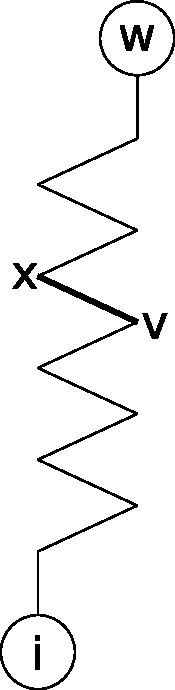
\includegraphics[scale=.4]{kap3DesZahlst}
  \caption{Die Ränge wachsen monton steigend von unten nach oben. Wenn sich die Ranggruppe von v und x unterscheidet, werden die Kosten der Find-Operation berechnet, sonst dem Knoten v.}
  \label{kap3DesZahlst}
\end{figure}

Keine \texttt{Find}"=Operation wird mit mehr als $G(n)$ Kosten belastet. Die Ränge sind laut der 4. Eigenschaft aufsteigend sortiert (monoton steigend). Die Ranggruppe kann sich höchstens $G(n)$ mal ändern, was der Anzahl der Ranggruppen entspricht. Eigentlich ändert sich die Ranggruppe sogar nur $G(\log{n})$ mal. Der Unterschied zwischen $G(n)$ und $G(\log n)$ ist höchstens $1$, da $G(\log n)$ den Logarithmus einmal mehr ausführt, als $G(n)$ dies bereits tut.

Wie viele Kosten fallen bei den Knoten selbst an? Betrachten wir Knoten $v$: Durch die Pfadkompression wird $v$ nach oben bewegt und wird Kind eines Vaters dessen Rang größer sein muss, als der seines bisherigen Vaters (wegen der monoton steigenden Ränge). Sei $g$ die Gruppe des Knotens $v$, also $g = G(Rang(v))$. Dann gibt es höchstens $F(g) - F(g-1)$ Ränge in der Gruppe g. Höchstens $F(g) - F(g-1)$ mal kann die Ranggruppe von $v$ der Ranggruppe seines Vaters entsprechen. Höchstens so oft kann also ein Knoten $v$ belastet werden.

Sei $N(g)$ die Anzahl der Knoten in Ranggruppe $g$. Wir können $N(g)$ bestimmen:
\[ N(g) \le \sum_{r=F(g-1)+1}^{F(g)}\frac{n}{2^r} \]
weil es laut der 2. Eigenschaft höchstens $\frac{n}{2^r}$ Knoten vom Rang $r$ gibt und es höchstens $F(g) - F(g-1)$ Ränge in Gruppe $g$ gibt. Wir können das umformen:
\begin{align*}
N(g) &\le \sum_{r=F(g-1)+1}^{F(g)}\frac{n}{2^r}\\
     &= \frac{n}{2^{F(g-1)+1}} (1 + \frac{1}{2} + \frac{1}{4} + \ldots)\\
     &\le \frac{n}{2^{F(g-1)}} \cdot \frac{1}{2} \cdot 2\\
     &= \frac{n}{2^{F(g-1)}} \\
     &= \frac{n}{F(g)}
\end{align*}

Es gibt also höchstens $\frac{n}{F(g)}$ Knoten in Ranggruppe $g$, die jeweils höchstens $F(g) - F(g-1) < F(g)$ mal belastet werden. Ranggruppe $g$ wird also maximal $\frac{n}{F(g)} \cdot F(g)$ mal belastet. Da es nicht mehr als $G(n)$ Ranggruppen gibt, liegen die Gesamtkosten aller Knoten in $\mathcal{O}(n \cdot G(n))$.

\begin{Satz}
  \hspace{\parindent}Ausgehend von einer Partition $S_i = \{ i \}$ mit $i = 1, \ldots , n$ wird eine Folge $\sigma$ ausgeführt, bestehend aus $\le n$ \texttt{Union}"=Operationen nach Rang und $m$ \texttt{Find}"=Operationen mit Pfadkompression. Die Gesamtlaufzeit von $\sigma$ liegt dann in $\mathcal{O}(n \log^*n + m \log^*n) = \mathcal{O}((n+m) \log^* n)$.
\end{Satz}

Aus diesem Satz folgt insbesondere, dass \texttt{Find} mit Pfadkompression eine amortisierte Laufzeit von $\mathcal{O}(\log^* n)$ hat.

Es sei noch angemerkt, dass es sogar noch schneller geht, auch wenn wir das im Folgenden nicht beweisen. Zunächst führen wir jedoch die \textit{Ackermann"=Funktion} ein: $A: \mathbb{N} \times \mathbb{N} \to \mathbb{N}$, definiert durch:
\begin{align*}
  A(0,0) &= 0\\
  A(i,0) &= 1 \quad i\ge 1 \\
  A(0,x) &= 2x \quad x \ge 0\\
  A(i+1, x) &= A(i, A(i+1, x-1))
\end{align*}

Daraus folgt:
\begin{align*}
  A(1,x) &= A(0, A(1, x-1)) = 2 \cdot A(1,x-1)\\
  A(2, x) &= A(1, A(2, x-1)) = 2^{A(2, x-1)}
\end{align*}

\begin{figure}[htb]
  \centering
  \begin{tabular}{l||>{$}r<{$}>{$}r<{$}>{$}r<{$}>{$}r<{$}>{$}r<{$}>{$}r<{$}}
%    \backslashbox[3em]{i}{x} & 0 & 1 & 2 & 3 & 4 & 5 \\\hline\hline
        & x=0 & x=1 & x=2 & x=3 & x=4 & x=5 \\\hline\hline
    $i=0$ & 0 & 2 & 4 & 6 & 8 & 10\\
    $i=1$ & 1 & 2 & 4 & 8 & 16 & 32\\
    $i=2$ & 1 & 2 & 4 & 16 & 65356 & \ldots\\
    $i=3$ & 1 & 2^2 & 2^{2^{2^{2}}} & \multicolumn{3}{l}{$2^{2^{\iddots^{2}}\big\} 65356}\quad\ldots$}
  \end{tabular}
  \caption{Einige Werte der Ackermann"=Funktion.}
  \label{AckermannWerte}
\end{figure}

$A(2,X)$ entspricht ungefähr $F(i)$. $A(z,4)$ wächst bereits viel stärker als $F(i)$.

Es gibt auch eine Funktion, die \textit{inverse Ackermann"=Funktion} genannt wird:
\[ \alpha(m, n) = min \{z \ge 1 \mid A(z, 4 \cdot \lceil\frac{m}{n}\rceil) > \log n\} \]

\begin{Satz}
  \hspace{\parindent}Ausgehend von einer Partition $S_i = \{ i \}$ mit $i = 1, \ldots , n$ wird eine Folge $\sigma$ ausgeführt, bestehend aus $\le n$ \texttt{Union}"=Operationen nach Rang und $m$ \texttt{Find}"=Operationen mit Pfadkompression. Die Gesamtlaufzeit von $\sigma$ liegt dann in $\mathcal{O}(m \cdot \alpha(m,n))$.
\end{Satz}

Den Beweis führen wir hier nicht.

%vorlesung 12 vom 29.11.2010
\chapter{Graphenalgorithmen}
\section{Einführung}
\subsection{Definitionen}
\begin{Def}[Graph]
  \hspace{\parindent}Ein \textit{Graph} $G=(V, E)$ ist eine Menge von \textit{Knoten} $V$ und \textit{Kanten} $E$. Knoten werden auch Ecken oder englisch \textit{vertices} (von vertex) genannt, Kanten nennt man im Englischen \textit{edges}. Es gilt $E \subseteq \binom{V}{2}$, das heißt Kanten sind ungeordnete Paare über $V$.
\end{Def}

\begin{Def}[gerichteter Graph]
  \hspace{\parindent}Ein \textit{gerichteter Graph} ist ein Graph, in dem die Kanten definiert sind als $E \subseteq V \times V$ (geordnete Paare).
\end{Def}

\begin{Bsp}[gerichteter Graph]
  \hspace{\parindent}$V = \{1, \ldots, 7\} \quad E = \{(1,2), (2,2), (1,3), \ldots \}$
  
  \begin{figure}[htb]
    \centering
    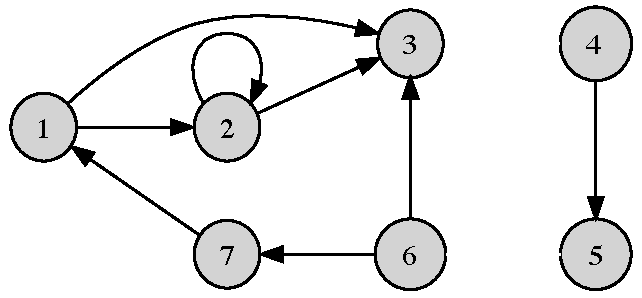
\includegraphics[scale=.5]{kap4Beispiel1}
    \caption{Ein gerichteter Graph}
    \label{kap4Beispiel1}
  \end{figure}
\end{Bsp}

\begin{Def}[Weg in einem Graphen]
  \hspace{\parindent}Ein \textit{Weg} in einem Graphen $G=(V,E)$ ist eine Folge von Knoten $v_1, \ldots, v_n$, wobei $(v_{i}, v_{i+1}) \in E$ für alle $i=1,\ldots n-1$. Die \textit{Länge eines Weges} ist $n-1$. Ein Weg $v_1, \ldots, v_n$ heißt \textit{einfach} genau dann, wenn $v_i \neq v_j$ für $i \neq j$ gilt.
\end{Def}

\begin{Def}[Kreis in einem Graph]
  \hspace{\parindent}Ein Weg $v_1, \ldots, v_n$ heißt \textit{Kreis} genau dann, wenn $v_1=v_n$. Ein Kreis heißt \textit{einfach}, wenn $v_i \neq v_{i+1}$ für alle $i=1, \ldots n-1$.
\end{Def}

\begin{Def}[azyklischer Graph]
  \hspace{\parindent}Ein Graph heißt \textit{azyklisch}, wenn er keinen Kreis enthält.
\end{Def}

\begin{Def}[zusammenhängender Graph]
  \hspace{\parindent}Ein ungerichteter Graph heißt \textit{zusammenhängend} genau dann, wenn zwischen je zwei Knoten $u,v \in V$ ein Weg $u=v_1, \ldots v_n = v$ existiert. Ein gerichteter Graph heißt \textit{stark zusammenhängend} genau dann, wenn zwischen je zwei Knoten $u,v \in V$ ein Weg $u=v_1, \ldots v_n = v$ existiert.
\end{Def}

\begin{Def}[Teilgraph]
  \hspace{\parindent}Ein Graph $G' = (V', E')$ heißt \textit{Teilgraph} eines Graphen $G=(V,E)$ genau dann, wenn $V' \subseteq V$ und $E' \subseteq E$. Ein Teilgraph heißt \textit{induzierter Teilgraph} genau dann, wenn $E' = E \bigcap (V' \times V')$ im gerichteten Fall und $E' = E \bigcap \binom{V'}{2}$ im ungerichteten Fall. Ein induzierter Teilgraph enthält also all die Kanten, die in $G$ zwischen den Knoten verlaufen, die auch in $V'$ enthalten sind.
\end{Def}

\begin{Def}[Zusammenhangskomponente]
  \hspace{\parindent}Eine \textit{Zusammenhangskomponente} von $G$ ist der maximale zusammenhängende induzierte Teilgraph $G' = (V', E')$. Maximal bedeutet, dass es keine echte Obermenge $V' \subsetneqq V''$ gibt, so dass der induzierte Teilgraph $G''=(V'', E'')$ zusammenhängend ist. Ist $G$ gerichtet, so spricht man von einer \textit{starken Zusammenhangskomponente}.
\end{Def}

\subsection{Darstellung endlicher Graphen}
Es gibt viele Möglichkeiten einen endlichen Graphen darzustellen, häufig genutzt werden die Adjazenzmatrix, die Adjazenzliste und die Inzidenzmatrix. Im folgenden gehen wir ohne Beschränkung der Allgemeinheit davon aus, dass der darzustellende Graph $G$ aus der Knotenmenge $\{ 1, \ldots, n \}$ besteht.

Eine \textit{Adjazenzmatrix} ist eine $n \times n$-Bitmatrix $A$. Für jeden Knoten enthält die Matrix eine Spalte und eine Zeile, dem entsprechend braucht eine Adjazenzmatrix $\Theta(n^2)$ Platz, mit $n = |V|$. $a_{ij} = 1 \Leftrightarrow (i,j) \in E$, die Matrix speichert also die zwischen Knoten verlaufenden Kanten. In ungerichteten Graphen gilt $a_{ij} = a_{ji}$.

\textit{Adjazenzlisten} speichern zu jedem Knoten $v$ eine Liste aller adjazenten Knoten, also alle $u$ mit $(v, u) \in E$. Adjazenzlisten brauchen $\Theta(n + m)$ viel Platz, mit $n = |V|$ und $m = |E|$.

Eine \textit{Inzidenzmatrix} hat für jeden Knoten eine Zeile und für jede Kante eine Spalte. Jede Spalte kann maximal zwei Einträge beinhalten, die sich von $0$ unterscheiden. Im ungerichteten Fall wird $1$ bei Knoten $v$ und Kante $e$ eingetragen genau dann, wenn $v$ inzident zu $e$ ist, das heißt wenn $v$ einer der beiden Endpunkte von $e$ ist. Im Fall eines azyklischen gerichteten Graphen wird beim Startknoten eine $1$ eingetragen und beim Endknoten eine $-1$.

\begin{Def}[Grad eines Knotens]
  \hspace{\parindent}Der \textit{Grad} eines Knotens entspricht im ungerichteten Fall der Anzahl inzidenter Kanten. Im gerichteten Fall wird zwischen dem \textit{Ingrad} und dem \textit{Ausgrad} unterschieden.
\end{Def}

\begin{Def}[Traversieren von Graphen]
  \hspace{\parindent}Als \textit{traversieren} von Graphen bezeichnet man das systematische besuchen aller Knoten eines Graphen, in dem man entlang der Kanten läuft. Hierzu gibt es zwei Techniken: Breiten- und Tiefensuche.
\end{Def}

Die \textit{Breitensuche} (BFS, \textit{breadth first search}) durchsucht $G=(V, E)$ bei $v$ beginnend. BFS findet alle direkten Nachbarn von $v$ und speichert sie in einer Warteschlange (Queue). Solange in der Warteschlange Knoten gespeicher sind, fügt es die noch nicht gefundenen Nachbarn des ersten Knotens der Warteschlange an die Warteschlange an. Dieser Vorgang wird solange wiederholt, bis die Warteschlange leer ist und keine unbekannten Knoten mehr gefunden werden. BFS findet kürzeste Wege in $G$, die von $v$ ausgehen. Die Laufzeit liegt in $\mathcal{O}(n^2)$, wenn $G$ als Adjazenzmatrix vorliegt und in $\mathcal{O}(n+m)$ bei der Darstellung von $G$ als Adjazenzliste.

Die \textit{Tiefensuche} (DFS, \textit{depth first search}) benutzt Rekursion oder einen Kellerspeicher (Stack). Alle Nachbarn eines Knotens $v$ werden darauf untersucht, ob sie bereits gefunden wurden. Die Knoten, die noch unbekannt sind werden in einen Speicher gelegt. Anschließend wird der oberste Knoten aus dem Kellerspeicher genommen und genauso untersucht. Dieses Verfahren wird angewandt, bis der Kellerspeicher leer und alle Knoten untersucht sind. Die Laufzeit liegt in $\mathcal{O}(n^2)$, wenn der zu untersuchende Graph als Adjazenzmatrix dargestellt wird, beziehungsweise in $\mathcal{O}(n+m)$ bei der Darstellung als Adjazenzliste. Die Tiefensuche findet alle Knoten zu denen es einen Weg von $v$ aus gibt (im ungerichteten Graphen ist das genau die Zusammenhangskomponente, die $v$ enthält).

Speichert man die Reihenfolge, in der die Knoten bei der Breiten- oder Tiefensuche entdeckt werden, kann man einen BFS-Baum beziehungsweise einen DFS-Baum aufstellen. Die Nummern der Reihenfolge (BFS- beziehungsweise DFS-Nummer) ist nicht eindeutig: Hat ein Knoten $v$ mehr als einen Nachbarn, wird bei BFS und DFS zufällig entschieden, welcher der Nachbarn zuerst besucht wird.

\begin{figure}[hbt]
  \centering
  \subfloat[\label{kap4BfsDfsBaum}]{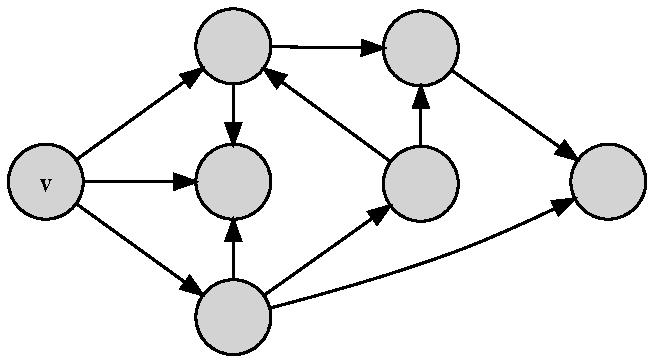
\includegraphics[width=.45\textwidth]{kap4BfsDfsBaum}}\\
  \subfloat[\label{kap4BfsBaum}]{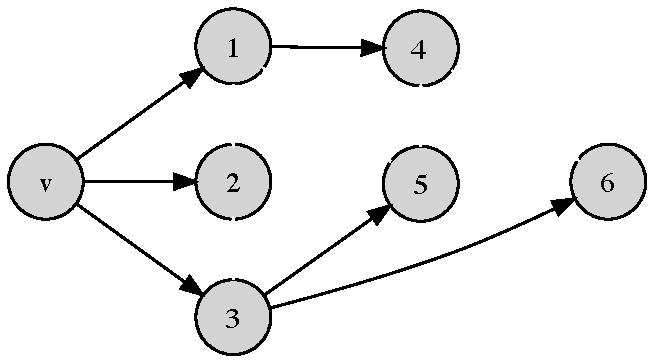
\includegraphics[width=.45\textwidth]{kap4BfsBaum}}\hspace{.05\textwidth}
  \subfloat[\label{kap4DfsBaum}]{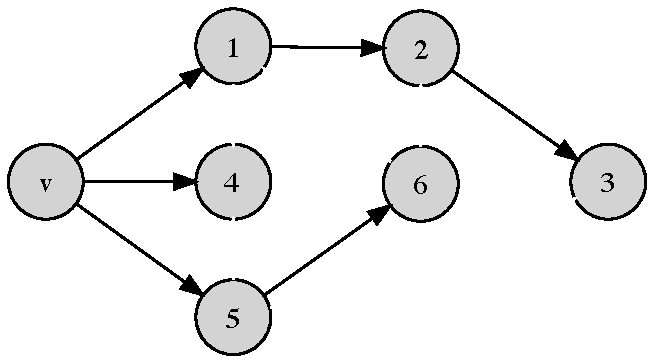
\includegraphics[width=.45\textwidth]{kap4DfsBaum}}
  \caption{\subref{kap4BfsDfsBaum} zeigt einen Graphen, \subref{kap4BfsBaum} einen zugehörigen BFS-Baum und \subref{kap4DfsBaum} einen zugehörigen DFS-Baum. In den DFS- und BFS-Baum sind die BFS- bzw. DFS-Nummern der Knoten eingetragen. BFS-Bäume enthalten kürzeste Wege vom Startknoten $v$ zu jedem anderen im Baum enthaltenen Knoten, so alle Kantenkosten identisch sind.}
  \label{kap4BfsDfsBaeume}
\end{figure}

\section{Minimale Spannbäume}
Gegeben ist ein ungerichteter Graph $G=(V,E)$ und eine Kostenfunktion $c: E \to \mathbb{R_+}$, die jeder Kante des Graphen Kosten zuweist. Gesucht ist ein zusammenhängender azyklischer Teilgraph $G'=(V, E')$ mit minimalen Gesamtkosten.

\begin{figure}[htb]
  \centering
  \subfloat[\label{kap4MST1}]{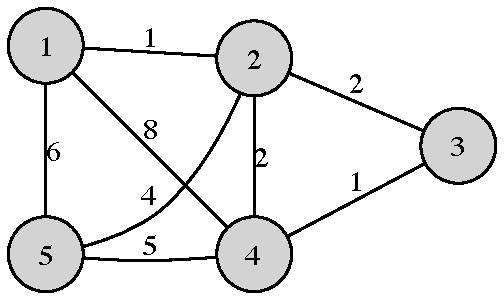
\includegraphics[width=.4\textwidth]{kap4MST1}}\hspace{.05\textwidth}
  \subfloat[\label{kap4MST2}]{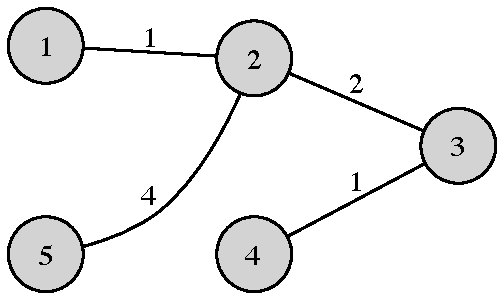
\includegraphics[width=.4\textwidth]{kap4MST2}}
  \caption{\subref{kap4MST2} ist ein minimaler Spannbaum des Graphen aus Abbildung \subref{kap4MST1}.}
  \label{kap4MST}
\end{figure}

\begin{Def}[Baum]
\hspace{\parindent}Ein \textit{Baum} ist ein azyklischer, zusammenhängender Graph.
\end{Def}

\begin{Def}[Spannbaum]
\hspace{\parindent}Ein \textit{Spannbaum} des Graphen $G=(V,E)$ ist ein Teilgraph $T=(V, E')$, der ein Baum (azyklisch, zusammenhängend) ist.
\end{Def}

Der \textit{Algorithmus von Kruskal} dient dem Finden von Spannbäumen minimaler Kosten. Er beginnt mit einem "`Spannwald"' $\{v_1\} \ldots \{v_n\}$.

\begin{Alg}[Algorithmus von Kruskal]
\begin{algorithmic}[1]
  \State $T := \emptyset$
  \State $Q := E$ \Comment{Prioritätswarteschlange gemäß Kosten}
  \State $VS := \{ \{v_1\} \ldots \{v_n\} \}$ \Comment{Partition der Knotenmenge}
  \While{$|VS| > 1$}
    \State $e:=\text{\texttt{delete-min}}(Q)$
    \If{$u, v$, mit $e=(u,v)$, liegen nicht in der gleichem Menge der Partion $VS$}
      \State Vereinige in $VS$ die Mengen, die $u$ und $v$  enthalten
      \State $T := T \cup \{ e \}$
    \EndIf
  \EndWhile
\end{algorithmic}
\end{Alg}

Als Datenstruktur für $Q$ bietet sich ein Heap an. Für $VS$ nutzen wir eine Union"=Find"=Struktur, mittels \texttt{Find} lässt sich leicht feststellen, ob $u$ und $v$ in der gleichen Menge der Partition liegen oder nicht, mit \texttt{Union} lassen sich bei Bedarf die Mengen, in denen $u$ und $v$ liegen leicht vereinigen. Die Initialisierung in Zeile $2$ liegt also in $\mathcal{O}(m \log m)$, die von Zeile $3$ in $\mathcal{O}(n)$. Die Laufzeit von Zeile 5 liegt in $\mathcal{O}(\log m)$ und wird $m$-mal ausgeführt, liegt insgesamt also in $\mathcal{O}(m \log m)$. Die Laufzeit der Zeilen 6 und 7 liegt insgesamt in $\mathcal{O}((n+m) \log^{*}n)$. Insgesamt liegt die Laufzeit des Algorithmus von Kruskal also in $\mathcal{O}(m \log m)$.

Der Algorithmus von Kruskal folgt einer einfachen Strategie, die als \textit{Greedy-Strategie} bekannt ist. Er sortiert alle Kanten nach ihren Kosten. Er betrachtet sich dann die jeweils günstigste noch nicht betrachtete Kante. Liegen die beiden Endknoten der Kante in unterschiedlichen Zusammenhangskomponenten, so fügt er die Kante zu seiner Lösung hinzu und vereinigt damit die beiden Zusammenhangskomponenten.

Der Algorithmus von Kruskal nimmt immer die nächste günstigste Kante. Die Strategie eines Algorithmus immer das nächste Beste zu bearbeiten nennt man \textit{greedy} (gierig). Auf abstrakte Strukturen verallgemeinernd können wir festhalten: greedy Algorithmen funktionieren auf \textit{Matroiden}.

%\section{Wegeprobleme in gerichteten Graphen}
%Gegeben sind ein gerichteter Graph $G=(V, E)$ und eine Kostenfunktion $c : E \to \mathbb{R}$. Häufig gestellte Fragen sind dann:
%
%\begin{enumerate}\renewcommand{\labelenumi}{\alph{enumi})}
%  \item Finde einen Weg mit minimalen Kosten, von $u$ nach $v$, mit $u,v \in V$.
%  \item Finde alle Wege mit minimalen Kosten von einem Knoten $u \in V$ zu jedem $v \in V$. Dieses Problem nennt man \textit{SSSP} (\textit{single source shortest path}).
%  \item Finde Wege mit minimalen Kosten zwischen allen Knotenpaaren $u, v$. Diese Fragestelltung wird \textit{APSP} (\textit{all pairs shortest path}) genannt.
%\end{enumerate}

%SSSP: Algorithmus von Daijkstra kurz erklären

%vorlesung 13 03.12.2010 (Fr)
%Ehe wir uns mit kürzesten"=Wege"=Problemen beschäftigen, sollten wir uns von der Korrektheit des Kruskal-Algorithmus überzeugen.

\subsection{Korrektheit des Kruskal"=Algorithmus (Greedy)}
Warum arbeitet der Algorithmus von Kruskal korrekt (beliebte Frage in Prüfungen)?

\begin{Lma}\label{kap4LmaKruskal}
\hspace{\parindent}Gegeben sind ein ungerichteter gewichteter Graph $G=(V, E)$ und ein aufspannender Wald $(V_1, T_1) \ldots (V_k, T_k)$ und $T=T_1 \cup \ldots \cup T_k$. Sei $e=(u,v)$ eine Kante mit minimalen Kosten und $u \in V_1$, $v \notin V_1$. Dann existiert der aufspannende Baum von $G$, der $T \cup \{e\}$ enthält und minimale Kosten unter allen Bäumen hat, die $T$ enthalten.
\end{Lma}

\begin{figure}[htb]
  \centering
  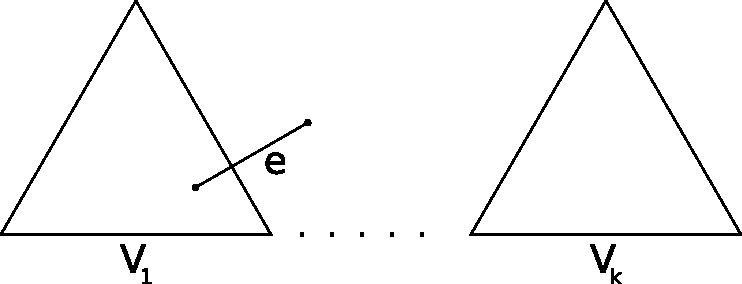
\includegraphics[scale=.5]{kap4KruskalErkl1}
  \caption{Die Ausgangslage des Lemmas \vref{kap4LmaKruskal}.}
  \label{KruskalErkl1}
\end{figure}

Aus Lemma \vref{kap4LmaKruskal} folgt die Korrektheit des Kruskal"=Algorithmus durch Induktion über seine Schleife.
Wir zeigen: jeder Wald, der bei Kruskals Algorithmus entsteht, ist Teilgraph eines minimal aufspannenden Baumes. Als Induktionsanfang dient uns bereits die Ausgangslage von Kruskals Algorithmus. Nach $0$ Iterationen besteht der Wald aus einem einzelnen Knoten.

Es folgt der Iterationsschritt von $k$ Iterationen auf $k+1$ Iterationen. Die Bäume $(V_1, T_1) \ldots (V_k, T_k)$ sind Teilgraphen eines minimal spannenden Baums (MST, \textit{minimum spanning tree}) nach Induktionsvoraussetzung. $e$ sei Kante minimalen Gewichts, die aus einem $V_i$ herausführt. Wenn man sie hinzu nimmt, dann gibt es nach Lemma \ref{kap4LmaKruskal} immer noch einen MST, der $T_1 \cup \ldots \cup T_k \cup \{e\}$ enthält. Es bleibt das Lemma zu Beweisen.

\begin{Bew}[Lemma \ref{kap4LmaKruskal}]
  \hspace{\parindent}Sei $B$ ein aufspannender Baum, der $T$ enthält und unter den Bäumen, die $T$ enthalten, minimale Kosten hat. Falls $e \in B$ ist das Lemma erfüllt. Andernfalls füge $e$ in $B$ ein. Es entsteht ein Kreis, denn $B$ enthält eine Kante $e' = (u', v')$ mit $u' \in V_1$, $v' \notin V_1$ und $e' \neq e$.  Es folgt $c(e) \le c(e')$ da $e$ minimal mit dieser Eigenschaft war.
  
  \begin{figure}[htb]
    \centering
    \includegraphics[scale=.32]{kap4BewKruskalLma}
    \caption{Wir sehen den Graphen $G$, sowie die Teilgraphen $V_1, \ldots, V_k$. $V_1$ ist ein aufspannender Baum, der $T$ enthält. Fügen wir nun eine Kante $e=(u,v)$ mit $u \in V_1$ und $v \notin V_1$ hinzu, gibt dies einen Kreis, da er bereits eine Kante $e'=(u', v')$ mit $u' \in V_1$ und $v \notin V_1$ enthält: Da $V_1$ ein Baum ist gibt es einen Weg von $u$ nach $u'$. Außerdem gibt es einen Weg von $v$ nach $v'$ (im Zweifelsfall über die Wurzel von $G$).}
  \end{figure}
  
  Wir schaffen nun einen neuen aufspannenden Baum $B'$, indem wir in $B$ $e'$ durch $e$ ersetzen. $B'$ enthält dann $T \cup \{e\}$. Es gilt $c(B') \le c(B)$, also ist $c(B')$ auch minimal unter Bäumen die $T$ enthalten (genau genommen gilt sogar $c(e) = c(e')$ und $c(B) = c(B')$).
\end{Bew}


\section{Wegeprobleme in gerichteten Graphen}
Gegeben ist im Allgemeinen ein gerichteter Graph $G=(V, E)$ mit Kostenfunktion $c : E \to \mathbb{R}$. Häufig gestellte Fragen sind dann:

\begin{itemize}\renewcommand{\labelenumi}{\alph{enumi})}
  \item Finde einen Weg mit minimalen Kosten, von $u$ nach $v$, mit $u,v \in V$.
  \item Finde Wege mit minimalen Kosten von einem Knoten $u \in V$ zu jedem anderen Knoten $v \in V$. Dieses Problem nennt man \textit{SSSP} (\textit{single source shortest path}).
  \item Finde Wege mit minimalen Kosten zwischen allen Knoten. Dieses Problem wird \textit{APSP} (\textit{all pairs shortest path}) genannt.
\end{itemize}

Wege mit minimalen Kosten werden manchmal auch \textit{kürzeste Wege} genannt. Als \textit{kürzesten Weg} kann man aber auch den Weg verstehen, der am wenigsten Kanten enthält. Im folgenden sprechen wir vom kürzesten Weg auch wenn wir den günstigsten Weg meinen. Aus dem Zusammenhang sollte eh hervorgehen, was gemeint ist (ein ungewichteter Graph entspricht einem gewichtetem Graph, bei dem alle Kantengewichte gleich sind).

\subsection{Dijkstras Algorithmus}
SSSP lässt sich mit Dijkstras Algorithmus lösen. Diesen Algorithmus wollen wir im folgenden vorstellen. Dabei bezeichnet $c[i,j]$ die Kosten der Kante $(i,j)$ falls $(i,j) \in E$. Es gilt $c[i,j] = \infty$ falls $(i,j) \notin E$. In $S$ speichern wir die Kontenmenge der Knoten zu denen bereits kürzeste Wege gefunden wurden. $D[v]$ bezeichnet die Kosten des kürzesten Weges von $s$ nach $v$.

\begin{Alg}[Dijkstra"=Algorithmus]
\begin{algorithmic}[1]
  \State $S :	= \emptyset$
  \State $D[s] := 0$
  \ForAll{$v \in V \setminus \{s\}$}
%    \State $D[v] := c[s,v]$
    \State $D[v] := \infty$
  \EndFor
  \While{$|S| < n$}
    \State wähle Knoten $w$ mit $w \in V \setminus S$ und $D[w]$ ist minimal
    \State $S := S \cup \{ w \}$
    \ForAll{$u \in V \setminus S$ und $u$ adjazent zu $w$}
      \State $D[u] := min(D[u], D[w] + c(w,u))$
    \EndFor
  \EndWhile
\end{algorithmic}
\end{Alg}

\subsubsection{Korrektheit von Dijsktra}
\begin{Beh}
  \hspace{\parindent}Zu jedem Zeitpunkt nachdem ein Knoten $w \in V$ in $S$ aufgenommen wird (Zeile 8) entspricht $D[w]$ genau der Länge des kürzesten Weges von $s$ nach $w$.
\end{Beh}

\begin{Bew}
  \hspace{\parindent}Der Beweis erfolgt per Induktion über die Anzahl $k$ der Iterationen der while-Schleife (Zeilen 6--12). Als Induktionsanfang wählen wir $k=0$. $S$ entspricht dann der leeren Menge, die Behauptung ist erfüllt. Wir können auch $k=1$ betrachten. Der Dijkstra"=Algorithmus wählt den Knoten $s$, es gibt keinen Knoten, der s näher sein kann, als s selbst. Der Abstand von s zu sich selbst entspricht $D[s] = 0$.
  
  Ehe wir den Induktionsschritt betrachten, führen wir noch $d(w)$ ein. $d(w)$ steht für die tatsächlichen Kosten des kürzesten Weges von $s$ nach $w$. In der $k$-ten Iteration der While"=Schleife werde $w$ aufgenommen. Wir nehmen an, dass wir den kürzesten Weg von $s$ nach $w$ noch nicht gefunden haben, das heißt $d(w) < D[w]$.
  
  \begin{figure}[htb]
    \centering
    \includegraphics[scale=.66]{kap4DijkstraKorrekt}
    \caption{Betrachten den tatsächlich kürzesten Weg $\pi$ von $s$ nach $w$: $\pi$ verlässt die Menge $S_{k-1}$ zum ersten Mal beim Traversieren der Kante $(u, v)$.}
    \label{kap4DijkstraKorrekt}
  \end{figure}
  
  Betrachten wir den tatsächlich kürzesten Weg $\pi$ von $s$ nach $w$. $\pi$ verlässt die Menge $S_{k-1}$ zum ersten Mal beim Traversieren der Kante $(u,v)$. Das Stück von $\pi$ bis $u$ ist der kürzeste Weg von $s$ nach $u$. Nach Induktionsvoraussetzung ist seine Länge $d(u) = D[u]$.
  
  Es muss gelten $d(v) \le d(u) + c(u,v) = D[u] + c(u,v) \ge D[v]$, denn $D[v]$ wurde auf $min(D[v], D[u] + c(u,v))$ gesetzt als $u$ in $S$ aufgenommen wurde. Tatsächlich gilt $D[v] = d(v)$, denn $d(u) + c(u,v)$ ist Teil des tatsächlich kürzesten Wegs $\pi$ von $s$ nach $w$. Des Weiteren muss gelten $D[w] \ge d(w) > d(v) = D[v]$. Dass steht aber im Widerspruch zum Dijkstra"=Algorithmus, der in Zeile 7 $w$ danach ausgesucht hat, dass $D[w]$ minimal ist.
  
  Somit haben wir bewiesen: zu jedem Zeitpunkt nachdem Knoten $w \in V$ in $S$ aufgenommen wird (Zeile 8) ist $D[w]$ die Länge des kürzesten Weges von $s$ nach $w$. Der Dijkstra"=Algorithmus arbeitet also korrekt.
\end{Bew}

\subsubsection{Laufzeit des Dijkstra"=Algorithmus}
Um eine Aussage über die Laufzeit des Dijkstra"=Algorithmus treffen zu können, müssen wir uns kurz überlegen, welche Datenstrukturen wir nutzen. Für die Knoten in $V \setminus S$ nutzen wir eine Prioritätswarteschlange (Heap) gemäß des Wertes $D$, alle anderen Datenstrukturen sollten trivial sein. Die Laufzeit für die Initialisierung (Zeilen 2--5) liegt in $\mathcal{O}(n)$. Zeile 7 und 8 entsprechen einem Aufruf von \texttt{delete"=min}, liegen also in $\mathcal{O}(\log n)$. Sie werden $n$ mal aufgerufen, was insgesamt in $\mathcal{O}(n \log n)$ liegt. Zeile 10 entspricht einem Aufruf von \texttt{decrease"=key} und liegt somit in $\mathcal{O}(\log n)$. Sie wird höchstens einmal pro Kante ausgeführt, was insgesamt in $\mathcal{O}(m \log n)$ liegt. Die Laufzeit des gesamten Algorithmus liegt also in $\mathcal{O}((n+m)\log n)$.

\subsection{All Pairs Shortest Path (APSP)}
Möchte man die kürzesten Wege zwischen allen Knoten berechnen, so könnte man einfach den Dijkstra"=Algorithmus auf alle Knoten anwenden. Von der Laufzeit her ist das aber nicht besonders gut, es läge in $\mathcal{O}(n (n+m) \log n)$, was sich mit $\mathcal{O}(n^3 \log n)$ abschätzen lässt. Geht das schneller?

%Algorithmus von Floyd"=Warshall
%
%$G(V,E)$
%$V=\{1, \ldots, n\}$
%$c(i,j)= Kosten von (i,j) fall (i,j) \in E, \infty sonst$.
%
%berechnen Werte
%$d_{ij}^k$ $\Big\{$ \begin{tabular}{l}$1\le i,j \le n$ \\ $0 \le k \le n$\end{tabular}
%
%= Länge des kürzesten Weges von $i$ nach $j$ mit Zwischenkonten in $\{1, \ldots k\}$ $\infty$ falls kein solcher Weg existiert.
%
%$d_{ij}^0 = c(i, j)$
%
%$d_{ij}^k$ Zeichnung 13-4
%erste Möglichkeit $k$ kommt nicht vor auf kürzestem Weg von $i$ nach $j$ mit Zwischenknoten $\in \{1, \ldots, k\}$: $d_{ij}^k = d_{ij}^{k-1}$
%
%$d_{ij}^k := min(d_{ij}^{k-1}, d_{ik}^{k-1}, d_{kj}^{k-1})$
%2. Möglichkeit $k$ kommt vor (ohne weitere Einschränkung nur einmal) Zeichnung 13-4b dann $d_{ij}^k = d_{ik}^{k-1} + d_{kj}^{k-1}$

% vorlesung 14 vom 06.12.2010 (Mo)
%APSP

Sei $G=(V,E)$ ein gerichteter Graph mit Kostenfunktion $c: E \to \mathbb{R}_{\ge 0}$. Die Knotenmenge $V$ sei o.B.d.A. $\{1, \ldots, n\}$. $d_{ij}^{k}$ entspricht den Kosten des kürzesten Weges zwischen $i$ und $j$ mit Zwischenknoten $\in \{1, \ldots, k\}$. $d_{ij}^k$ ist entweder $d_{ij}^{k-1}$ oder $d_{ik}^{k-1} + d_{kj}^{k-1}$. Ein Algorithmus, der die Kosten aller kürzesten Wege unter Nutzung der Methode des dynamischen Programmierens berechnet, ist dann einfach zu finden.

\begin{Alg}[von Floyd"=Warshall (dynamisches Programmieren)]
  \begin{algorithmic}[1]
    \For{$i=1 \ldots n$}
      \For{$j=1 \ldots n$}
        \If{$(i,j) \in E$}
          \State $d_{ij}^0 = c(i,j)$
        \Else
          \State $d_{ij}^0 = \infty$
        \EndIf
      \EndFor
    \EndFor
    \For{$k=1 \ldots n$}
      \For{$i=1 \ldots n$}
        \For{$j=1 \ldots n$}
          \State $d_{ij}^k = min(d_{ij}^{k-1}, d_{ik}^{k-1} + d_{kj}^{k-1})$\label{kap6FWAlgEntfernungBerechnen}
        \EndFor
      \EndFor
    \EndFor
  \end{algorithmic}
\end{Alg}

%Algorithmus von Floyd"=Warshall (dynamisches Programmieren)
%
%for $i=1, \ldots, n$ do\\
%  for $j=1, \ldots, n$ do\\
%    $d_{ij}^0$ = $c(i,j)$ falls $(i,j) \in E$, $\infty$ sonst\\
%  done\\
%done\\
%for $k=1, \ldots, n$ do\\
%  for $i=1, \ldots n$ do\\
%    for $j=1, \ldots, n$ do\\
%      $d_{ij}^k = min (d_{ij}^{k-1}, d_{ik}^{k-1} + d_{kj}^{k-1})$\\
%    done\\
%  done\\
%done\\

Die Länge der tatsächlich kürzesten Wege finden wir dann in $d_{ij}^n$ mit $1 \le i, j \le n$. Die Laufzeit liegt aufgrund der dreifach verschachtelten Schleife in $\mathcal{O}(n^3)$. Für mehrfaches Ausführen des Dijkstra"=Algorithmus hatten wir eine Laufzeit von $\mathcal{O}(n (n+m) \log n)$ angegeben. Die Anzahl der Kanten $m$ kann maximal $n^2$ groß werden. In einem vollständigen Graphen hat das dann eine Laufzeit von $\mathcal{O}(n^3 \log n)$, hier ist also der Algorithmus von Floyd"=Warshall günstiger. Für dünn besetzte Graphen (mit maximal $\frac{n^2}{n \log n}$ Kanten) ist das mehrfache Ausführen des Dijkstra"=Algorithmus jedoch besser.

Tatsächlich lassen sich mit beiden Algorithmen nicht nur die Länge der kürzesten Wege bestimmen, sondern auch die Wege selber (Teil der Übung). Der Algorithmus von Floyd"=Warshall ist vielseitig anwendbar. Setzt man in der Initialisierung $c(i,j) = 0$ falls $(i,j) \notin E$ und $1$ andernfalls und ersetzt die die Operanden $min, +$ durch $\vee$ und $\wedge$, so berechnet der Algorithmus, ob es überhaupt einen Weg zwischen zwei Knoten gibt, er berechnet also den transitiven Abschluss des Graphen $G$.

Der Algorithmus von Floyd"=Warshall geht ursprünglich auf einen Algorithmus von Kleene zurück. Eigentlich ist der Algorithmus von Floyd"=Warshall eine Abwandlung des Algorithmus von Kleene, wir beschreiben den Algorithmus von Kleene hier dennoch wie eine Abwandlung des Floyd"=Warshall"=Algorithmus.

Der Algorithmus bekommt als Eingabe einen endlichen Automaten (DFA) und gibt den regulären Ausdruck aus, der der Sprache entspricht, die der DFA erkennt. Die Zustände des Automaten werden dabei als Knoten angesehen und die Kostenfunktion als Abbildung von Kanten auf Elemente des Alphabets, also $c: E \to \Sigma$. $d_{ij}^k$ entspricht der Menge von Wörtern, die der Automat erzeugen kann, wenn er in Zustand $i$ beginnt, in Zustand $j$ endet und nur die Zustände $1, \ldots, k$ nutzt. Dazu wird die Initialisierung geändert zu:
\[ d_{i,j}^0 = \begin{cases}
                 a^* & \text{falls $i=j$ und der DFA erzeugt $a$ auf dem Weg von $i$ nach $i$}\\
                 \{ \varepsilon \} & \text{falls $i=j$ und } (i,i) \notin E\\
                 b & \text{falls $i \neq j$ und } (i,j) \in E \\
                 \emptyset & \text{sonst}
\end{cases} \]
und Zeile \ref{kap6FWAlgEntfernungBerechnen} des oben angegebenen Algorithmus von Floyd"=Warshall wird ersetzt durch
\[ d_{ij}^k = d_{ij}^{k-1} \cup d_{ik}^{k-1} (d_{kk}^{k-1})^* d_{kj}^{k-1} \]

\section{Flüsse in Netzen (network flow)}
Sei ein gerichteter Graph $G=(V,E)$ gegeben mit Kapazitätsfunktion $c: E \to \mathbb{R}_{\ge 0}$, \textit{Quelle} $s \in V$ und \textit{Ziel} (auch \textit{Senke} genannt) $t \in V$. Ein Beispiel eines solchen Graphen sehen wir in Abbildung \vref{kap4Fluesse1}. Gesucht wird der \textit{maximale Fluss} von $s$ nach $t$.

\begin{Def}[Netz]
  \hspace{\parindent}Wir definieren ein \textit{Netz} (oder auch \textit{Netzwerk}) $(V, E, c, s, t)$ als einen gerichteten Graphen mit Kapazitätsfunktion $c: E \to \mathbb{R}_{\ge 0}$, Quelle $s \in V$ und Senke $t \in V$.
\end{Def}

\begin{figure}[htb]
  \centering
  \includegraphics[scale=.75]{kap4Fluesse1}
  \caption{Ein Graph mit Quelle $s$ und Senkte $t$ und Kapazitäten an den Kanten.}
  \label{kap4Fluesse1}
\end{figure}

In der Praxis gibt es einige Beispiele: Röhrensysteme für Öl, Gas, Wasser oder ähnliches, Evakuierungspläne, Verkehrsnetze und so weiter.

\begin{Def}[Fluss]
\hspace{\parindent}Ein \textit{Fluss} ist eine Funktion $f: V \times V \to \mathbb{R}$ mit folgenden Eigenschaften:
\begin{alignat*}{2}
  f(u,v) & \le c(u,v) &\qquad& \text{wobei } c(u,v) := 0 \text{ falls } (u,v) \notin E\\
  f(u,v) & = -f(v,u) \\
  \sum_{v \in V} f(u,v) & = 0 && \forall u \in V \setminus \{s,t\}
\end{alignat*}
\end{Def}

\begin{Def}[Wert eines Flusses]
  \hspace{\parindent}Den \textit{Wert eines Flusses} definieren wir als
  \[|f| := \sum_{v \in V} f(s,v)\]
\end{Def}

\begin{figure}[htb]
  \centering
  \includegraphics[scale=.75]{kap4Fluesse2}
  \caption{In dem Beispiel aus Abbildung \vref{kap4Fluesse1} wurde mittels einer Greedy-Strategie ein maximaler Fluss bestimmt. Die Zahlen entlang der Kanten geben zuerst die durch den Fluss genutzte Kapazität dann die verfügbare Kapazität an. Der Fluss hat eine Größe von $|f| = 23$.}
  \label{kap4Fluesse2}
\end{figure}

Hat man ein Netzwerk mit mehr als einer Quelle und einer Senke, kann man das leicht auf eine Netzwerk mit einer Quelle und einer Senke zurückführen. Abbildung \vref{kap4MultQuellenSenken} zeigt wie das geht.

\begin{figure}[htb]
  \centering
  \includegraphics[scale=.75]{kap4MultQuellenSenken}
  \caption{Um ein Netzwerk mit mehr als einer Quelle und Senke zu einem Netzwerk mit einer Quelle und Senke zu wandeln führt man einen zusätzlichen Knoten $s$ und einen zusätzlichen Knoten $t$ ein. Von $s$ aus werden Kanten mit unendlich hoher Kapazität zu allen Quellen geführt und von den bestehenden Senken ebensolche Kanten zum Knoten $t$. $s$ wird dann Superquelle und $t$ Supersenke genannt.}
  \label{kap4MultQuellenSenken}
\end{figure}

\subsection{Ford"=Fulkerson"=Methode zur Bestimmung des maximalen Flusses}
Wie oben geschrieben suchen wir nach dem maximalen Fluss in einem solchen Netzwerk. Eine Methode dazu stammt von Ford und Fulkerson. Dazu wird im Netzwerk nach augmentierenden Wegen gesucht.

\begin{Def}[Augmentierender Weg]
  \hspace{\parindent} Gegeben ist ein Netzwerk mit einem Fluss $f$. Darin gibt es einen Weg von $s$ nach $t$, wobei für alle Kanten $(u,v)$ auf dem Weg gilt $f(u,v) < c(u,v)$. Das heißt alle Kanten auf dem Weg haben größere Kapazitäten, als sie bislang vom Fluss genutzt werden. Einen solchen Weg nennt man \textit{augmentierend}.
\end{Def}

\strut\begin{Alg}[Ford-Fulkerson]
  \begin{algorithmic}[1]
    \State initialisiere $f$ mit $0$ (auf jeder Kante).
    \While{augmentierender Weg exisitert}
      \State erhöhe den Fluss entlang dieses Weges so stark wie möglich.
    \EndWhile
  \end{algorithmic}
\end{Alg}

Beim Ausführen des Algorithmus von Ford"=Fulkerson hilft eine Datenstruktur, die wir Restnetz nennen.
\begin{Def}[Restnetz]
  \hspace{\parindent}Sei $G=(V,E)$ ein Graph mit Kapazitätsfunktion $c$, mindestens zwei Knoten $s$ und $t$ die als Quelle und Senke dienen und einem Fluss $f$. Das \textit{Restnetz} $G_f$ ist ein Graph mit der Knotenmenge $V$ und folgenden Kanten. Sei $e=(u, v) \in E$ eine Kante aus $G$ mit Kapazität $c(e)=b$, von der der Fluss bereits $f(e)=a$ nutzt. Dann hat die Kantenmenge des Restnetzes $E_f$ zwei Kanten: $(u,v)$ und $(v,u)$. Die Kapazitäten bestimmen wir wie folgt:
  \[ c_f(u,v) = b-a \]
  \[ c_f(v,u) = a \]
  
  Ist $c(u,v) = f(u,v)$ und somit $b-a = 0$, kann die Kante $(u,v)$ im Restnetz auch weggelassen werden. Analog kann auch die Kante $(v,u)$ weggelassen werden, wenn $f(u,v)=0$, also $b-a = b$.
\end{Def}

\begin{figure}[htb]
  \centering
  \subfloat[Eine einfache Kante im Netzwerk (links) wird ersetzt durch zwei Kante im Restnetz (rechts).\label{kap4RestnetzKonstruktion1}]{
    \includegraphics[width=.25\textwidth]{kap4RestnetzKonstruktionA1}\hspace{4em}\includegraphics[width=.25\textwidth]{kap4RestnetzKonstruktionB1}}\\
  \subfloat[Bestehen im Netzwerk bereits zwei Kanten, so wird $a$ zur Rückwärtskante addiert.\label{kap4RestnetzKonstruktion2}]{
    \includegraphics[width=.25\textwidth]{kap4RestnetzKonstruktionA2}\hspace{4em}\includegraphics[width=.25\textwidth]{kap4RestnetzKonstruktionB2}}
  \caption{Zu sehen ist, wie Kanten des Netzwerkes bei der Konstruktion des Restnetzes ersetzt werden. $b$ bezeichnet die Kapazität einer Kante, $a$ die durch den Fluss genutzte Kapazität, $c$ die Kapazität einer im Netzwerk bestehenden Rückwärtskante.}
  \label{kap4RestnetzKonstruktion}
\end{figure}

Die Konstruktion der Kanten im Restnetz zeigt Abbildung \vref{kap4RestnetzKonstruktion}. Einen Fluss in unserem Beispielnetzwerk und das resultierende Restnetz zeigt Abbildung \vref{kap4FluesseRestnetz}.

\begin{figure}[htb]
  \centering
  \subfloat[\label{kap4Fluesse3}]{\includegraphics[width=.45\textwidth]{kap4Fluesse3}}\hspace{.025\textwidth}
  \subfloat[\label{kap4Fluesse4}]{\includegraphics[width=.45\textwidth]{kap4Fluesse4}}
  \caption{\subref{kap4Fluesse3} zeigt einen Fluss in unserem Beispielnetz. \subref{kap4Fluesse4} zeigt das resultierende Restnetz.}
  \label{kap4FluesseRestnetz}
\end{figure}

Ein augmentierender Weg in $G$ entspricht einem Weg von $s$ nach $t$ im Restnetz $G_f$. Der Ford"=Fulkerson"=Algorithmus kann somit vereinfacht werden:

\begin{Alg}[Ford"=Fulkerson mit Hilfsstruktur $G_f$]
  \begin{algorithmic}[1]
    \State $G_f := G$
    \While{finde Weg von $s$ nach $t$ in $G_f$}
      \State erhöhe Fluss entlang dieses Weges so weit wie möglich
      \State aktualisiere $G_f$
    \EndWhile
  \end{algorithmic}
\end{Alg}

Sind alle Kapazitäten im Netzwerk ganzzahlig, so sind es auch alle Kapazitäten im Restnetzwerk, da wir nur ganze Zahlen addieren und subtrahieren. Der Fluss wird dann in jeder Iteration des Algorithmus um mindestens $1$ erhöht, was wichtig für die Analyse der Laufzeit ist. Warum können wir o.B.d.A. annehmen, dass alle Kapazitäten ganzzahlig sind? Weil wir andernfalls alle Kapazitäten entsprechend erweitern könnten. Arbeiten wir nicht mit ausschließlich ganzzahligen Kapazitäten, kann es passieren, dass der Algorithmus nicht terminiert!

Betrachten wird die Laufzeit dieses Algorithmus. Dabei sei $|V| = n$ und $|E| = m$. Das Finden eines augmentierenden Weges entspricht dem Finden eines Weges von $s$ nach $t$ in $G_f$. Dies ist zum Beispiel durch Breiten- oder Tiefensuche in $\mathcal{O}(n+m)$ möglich. Wir können wie gesagt von ganzzahligen Kapazitäten und somit von einer Steigerung des Flusses je Iteration um mindestens $1$ ausgehen. Daraus folgt das maximal $|f^*|$ Iterationen nötig sind. Dabei ist $f^*$ der endgültige (maximale) Fluss. Die Laufzeit liegt also in $\mathcal{O}(|f^*| \cdot (m+n))$. $f^*$ kann exponentiell in der Eingabegröße sein, wenn die Kapazitäten als Binärzahlen gegeben sind. Ist eine Zahl in Binärdarstellung gegeben, so ist ihr Wert exponentiell ihrer Länge.

%vorlesung 15 2010-12-10 (Fr)

\begin{figure}[htb]
  \centering
  \includegraphics[scale=.66]{kap4FFWorstCase}
  \caption{Ein Netzwerk, in dem der Algorithmus von Ford"=Fulkerson unter Umständen eine schlechte Laufzeit aufweist (Beispiel für eine worst-case-Analyse).}
  \label{kap4FFWorstCase}
\end{figure}

%Bei jeder Augmentierung erhöht sich der Fluss um mindestens $1$. Insgesamt hat man also maximal $|f^*|$ Augmentierungen, wobei $|f^*|$ dem endgültigen (maximalen) Fluss entspricht. Eine Augmentierung benötigt $\mathcal{O}(n+m)$ Zeit mit zum Beispiel Tiefen- oder Breitensuche, insgesamt liegt der Algorithmus also in $\mathcal{O}(|f^*| \cdot (m+n))$. Das ist potentiell exponentiell in der Größe der Eingabe (ist eine Zahl in Binärdarstellung gegeben, so ist ihr Wert exponentiell ihrer Länge, hier geht es um die Form der Kapazitäten).

Abbildung \vref{kap4FFWorstCase} zeigt ein Netz, in dem es passieren kann, dass der Ford"=Fulkerson"=Algorithmus den Fluss um je $1$ erhöht, also $2000$ Augmentierungen braucht. Es ist klar, dass wir den Algorithmus entsprechend verbessern sollten, wie genau zeigen wir später.

\subsection{Schnitte}
\begin{Def}[Fluss zwischen zwei Knotenmengen]
  \hspace{\parindent}In einem Netzwerk $N=(V, E, c, s, t)$ seien $X, Y$ zwei Mengen von Knoten. Dann definieren wir den Fluss von $X$ nach $Y$ als
\[ f(X,Y) := \sum_{x \in X} \sum_{y \in Y} f(x,y) \]
\end{Def}

Durch nachrechnen liese sich leicht beweisen, dass bei Flüssen zwischen Knotenmengen folgendes gilt:
\begin{Lma}\label{Lemma41}
  \begin{alignat*}{2}
    f(X,X) &= 0 &\quad& \forall X \subset V\\
    f(X,Y) &= -f(Y,X) && \forall X,Y \subset V\\
    f(X \cup Y, Z) &= f(X,Z) + f(Y,Z) && \forall X,Y \subset V, X \cap Y = \emptyset\\
    f(Z, X \cup Y) &= f(Z,X) + f(Z,Y) && \forall X,Y \subset V, X \cap Y = \emptyset
  \end{alignat*}
\end{Lma}

\begin{Def}[Schnitt]
  \hspace{\parindent}Wir definieren den \textit{Schnitt eines Netzwerks} als eine Partition der Knotenmenge $V = S \cupdot T$ mit Quelle $s \in S$ und Senke $t \in T$. Es handelt sich also um zwei disjunkte Teilmengen, das heißt $S \cap T = \emptyset$.
\end{Def}

\begin{figure}[htb]
  \centering
  \includegraphics[scale=.75]{kap4DefSchnitt}
  \caption{Die Abbildung skizziert eine einfache Vorstellung eines Schnitts.}
  \label{kap4DefSchnitt}
\end{figure}

Den Fluss zwischen zwei Knotenmengen haben wir bereits definiert. Analog dazu definieren wir die Kapazität eines Schnitts:
\[c(S,T) = \sum_{x \in S} \sum_{y \in T} c(x,y)\]
und den Fluss eines Schnitts:
\[ f(S,T) = \sum_{x \in S} \sum_{y \in T} f(x,y) \]

\begin{Lma}\label{Lemma42}
  Für jeden Fluss $f$ und jeden Schnitt $S, T$ gilt: \[ f(S,T) = |f| \]
\end{Lma}

\begin{Bew}
  \begin{alignat*}{2}
    f(S,T) &= f(S, V) - f(S,S) &\quad& \text{ weil } f(S,V) = f(S,T) + f(S,S)\\
           &= f(S, V) && \text{ weil } f(S,S) = 0\\
           &= f(\{s\}, V) + f(S \setminus \{s\}, V)\\
%           &= |f| + \sum_{u\in S \setminus \{s\}} \sum_{v\in V} f(u,v)\\
           & = |f| && \text{ weil } f(S \setminus \{s\}, V) = 0 \text{ und } f(\{s\}, V) = |f|
  \end{alignat*}
\end{Bew}

\begin{Koro}
  \hspace{\parindent}Der Wert jedes Flusses $f$ ist nach oben beschränkt durch die Kapazität jedes beliebigen Schnittes $S, T$:
  \[ |f| \le c(S,T) \]
  Dies gilt für jeden Fluss $f$ und jeden Schnitt $S$, also auch für den maximalen Fluss und den minimalen Schnitt.
\end{Koro}

\begin{Satz}[maximaler Fluss - minimaler Schnitt]
  \hspace{\parindent}Sei $f$ ein Fluss in einem Netzwerk $(V, E, c, s, t)$. Sei $G_f$ das entsprechende Restnetzwerk. Dann sind folgende Aussagen äquivalent:
  \begin{enumerate}
    \item \label{kap4SatzMaxFMinS:fMax} $f$ ist maximal.
    \item \label{kap4SatzMaxFMinS:augWeg} Es gibt keine augmentierenden Wege.
    \item \label{kap4SatzMaxFMinS:minS} Es gibt einen Schnitt $S,T$ mit $|f| = c(S,T)$.
  \end{enumerate}
\end{Satz}

\begin{Bew}
  \hspace{\parindent}Aus \ref{kap4SatzMaxFMinS:fMax} folgt \ref{kap4SatzMaxFMinS:augWeg} offensichtlich. Laut Definition ist ein augmentierender Weg ein Weg von $s$ nach $t$ bei dem für alle Kanten gilt, dass ihre Kapazitäten größer als die durch den Fluss genutzten Kapazitäten sind. Da dieser Fluss maximal ist, kann man ihn nicht mehr erhöhen, es kann also keinen augmentierenden Weg geben.
  
  \begin{figure}[htb]
    \centering
    \includegraphics[scale=.5]{kap4SchnittWeg}
    \caption{Alle Kanten von $S$ nach $T$ entsprechen den Kapazitäten, die dem Fluss zur Verfügung stehen. Kein Fluss kann daher größer sein, als es der minimale Schnitt ist. Für alle $u \in S$ und alle $v \in T$ gilt, dass die Kapazitäten von $(u,v)$ voll ausgenutzt sind, wenn es einen maximalen Fluss gibt.}
    \label{kap4SchnittWeg}
  \end{figure}
  
  Aus \ref{kap4SatzMaxFMinS:augWeg} folgt \ref{kap4SatzMaxFMinS:minS}: Es gibt keine augmentierenden Wege, das heißt es gibt keinen Weg von $s$ nach $t$ im Restnetz. Sei $S := \{ s \} \cup \{v \in V \mid \text{ in } G_f \text{ gibt es einen Weg von $s$ nach $v$}\}$ und $T := V \setminus S$. Dann muss $s \in S$ und $t \in T$ gelten. $S, T$ ist dann ein Schnitt. Für alle $u \in S$ und $v \in T$ gilt $c(u,v) = f(u,v)$. Aus Abbildung \vref{kap4SchnittWeg} und Lemma \ref{Lemma42} folgt
  \[ |f| = f(S,T) = c(S,T) \]
  
      
  Aus \ref{kap4SatzMaxFMinS:minS} folgt \ref{kap4SatzMaxFMinS:fMax} ergibt sich aus obigen Korollar. $|f| \le c(S,T)$ gilt für alle Schnitte und alle Flüsse. Für den vorher definierten Schnitt muss $c(S,T)$ minimal sein. Aus $|f| = c(S,T)$ folgt, dass $c(S,T)$ minimal und $|f|$ maximal sein muss, $f$ also der maximale Fluss ist.
\end{Bew}

Aus \ref{kap4SatzMaxFMinS:augWeg} folgt die Korrektheit des Algorithmus von Ford"=Fulkerson. Aus \ref{kap4SatzMaxFMinS:minS} folgt dass der minimale Schnitt dem maximalen Fluss entspricht.

Betrachten wir noch einmal unser Beispiel aus Abbildung \vref{kap4Fluesse1}. Ein Minimaler Schnitt ist zum Beispiel $T = \{ v_2, t \}$ und $S = V \setminus T$. Dieser Schnitt hat eine Größe von $23$, also gilt für dieses Netz $|f^*| = 23$. Abbildung \vref{kap4Fluesse5} zeigt das Netzwerk und den Schnitt.

\begin{figure}[htb]
  \centering
  \includegraphics[scale=.75]{kap4Fluesse5}
  \caption{Die gestrichelte blaue Linie zeigt einen minimalen Schnitt der Größe $23$.}
  \label{kap4Fluesse5}
\end{figure}

\subsection{Edmonds"=Karp"=Algorithmus}
Im Algorithmus von Ford"=Fulkerson heißt es, dass ein augmentierender Weg gefunden werden soll. Wie dieser Weg gefunden werden soll ist nicht angegeben. Der Edmonds"=Karp"=Algorithmus ist eine Variante des Ford"=Fulkerson"=Algorithmus. Der augmentierende Weg wird dabei durch Breitensuche im Restnetz $G_f$ gefunden. Der so gefundene augmentierende Weg ist der kürzeste bezüglich der Anzahl der Kanten.

Die Laufzeit des Edmonds"=Karp"=Algorithmus zu bestimmen ist nicht ganz einfach. Sei $\delta_f(u,v)$ der Abstand (die Anzahl der Kanten des kürzesten Weges) zwischen $u,v \in V$ im Restnetz $G_f$. Dann gilt:
\begin{Lma}
  \hspace{\parindent}Beim Edmonds"=Karp"=Algorithmus gilt für alle Knoten $v \in V \setminus \{ s,t \}$: In jedem augmentierenden Schritt wächst der Abstand von $\delta_{f}(s,v)$ monoton.
\end{Lma}

\begin{Bem}
  \hspace{\parindent}$\delta_{f}(u,v)$ zählt die Kanten zwischen zwei Knoten im Restnetz $G_f$. Das heißt, wenn $\delta_{f}(u,v)$ sich ändert, muss mindestens eine Kante im Restnetz hinzugefügt oder entfernt worden sein. % Eine Kante im Restnetz wird nur unter bestimmten Änderungen des Flusses entfernt oder hinzugefügt (Nutzung einer zuvor ungenutzten Kante durch den Fluss, erhöhen des Flusses auf einer Kante bis zu ihrer vollen Kapazität, entfernen einer Kante aus dem Fluss, absenken des Flusses auf einer voll ausgelasteten Kante).% Eine Kante wird zum Restnetz hinzugefügt, wenn der Fluss auf einer komplett ausgelasteten Kante des Netzwerks abnimmt oder eine noch nicht genutzte Kante des Netzwerks in den Fluss einbezogen wird. Eine Kante wird aus dem Restnetz entfernt, wenn ihr Pendant im Netzwerk aus dem Fluss entfernt wird oder die durch den Fluss genutzte Kapazität einer Kante im Netzwerk auf die volle Kapazität der Kante ansteigt. % Wächst der Abstand im Restnetz zwischen $s$ und einem Knoten $v$ monoton, bedeutet das, dass die Anzahl der durch 
\end{Bem}

\begin{Bew}
  \hspace{\parindent} Das Lemma beweisen wir, in dem wir einen Beweis durch Widerspruch führen. $f$ bezeichne den Fluss vor einem Augmentierungsschritt, $f'$ den Fluss nach einem Augmentierungsschritt. Angenommen das Lemma gelte nicht und es existiere ein Augmentierungsschritt bei dem für mindestens einen Knoten $v$ $\delta_{f'}(s,v) < \delta_{f}(s,v)$ gelte. Unter allen Knoten, für die das gilt, wählen wir o.B.d.A. den Knoten als $v$, bei dem $\delta_{f'}(s,v)$ minimal sei. Gilt für einen Knoten $u$ $\delta_{f'}(s,u) < \delta_{f'}(s,v)$, so muss auch $\delta_f(s,u) \le \delta_{f'}(s,u)$ gelten, denn sonst hätten wir $u$ an Stelle von $v$ ausgewählt.
  
  $p' \leadsto u \to v$ sei der kürzeste Weg von $s$ nach $v$ in $G_{f'}$. $u$ ist also der direkte Vorgänge von $v$ auf diesem Weg. Das heißt $\delta_{f'}(s, u) < \delta_{f'}(s,v)$, also gilt $\delta_{f}(s,u) \le \delta_{f'} (s,u)$ (sonst hätten wir $u$ an Stelle von $v$ gewählt). Für die Kante $(u,v)$ gibt es im Fluss $f$ dann zwei Möglichkeiten: Entweder es gilt $f(u,v) < c(u,v)$ oder es gilt $f(u,v) = c(u, v)$.
  
  Falls $f(u,v) < c(u,v)$ folgt daraus, dass $(u,v)$ als Kante im Restnetz $G_f$ enthalten ist, der kürzeste Weg von $s$ nach $G_f$ also auf keinen Fall länger sein kann, als der Weg von $s$ nach $u$ und von dort nach $v$. Also $\delta_{f}(s,v) \le \delta_{f}(s,u) + 1$ ($+1$ für die Kante $u \to v$). Dann gilt $\delta_{f}(s, u) + 1 \le \delta_{f'}(s,u) +1 = \delta_{f'}(s,v)$. Daraus folgt aber $\delta_{f}(s,v) \le \delta_{f'}(s,v)$, was unsere Annahme zum Widerspruch führt!
  
  Betrachten wir den Fall $f(u,v) = c(u,v)$. In diesem Fall ist $(u,v)$ keine Kante in $G_f$, aber eine Kante in $G_{f'}$, das heißt der augmentierende Weg $p$ muss die Kante $(v,u)$ enthalten. Der Edomnds"=Karp"=Algorithmus erweitert den Fluss immer nur entlang kürzester Wege, $p$ muss also der kürzeste Weg von $s$ nach $t$ im Restnetz $G_{f}$ sein, also ist $(v, u)$ Teil des kürzesten Wegs von $s$ nach $u$. Also
    \begin{align*}
      \delta_f(s,v) &= \delta_f(s,u) - 1 \\
                    &\le \delta_{f'}(s,u) -1 \\
                    &= \delta_{f'}(s,v) -2\\
                    &< \delta_{f'}(s,v)
    \end{align*}
    $\delta_f(s,v) < \delta_{f'}(s,v)$ ist ein Widerspruch zu unserer Annahme, das Lemma somit bewiesen.
\end{Bew}

Nachdem wir bewiesen haben, dass der Abstand zwischen einem Knoten $v$ (mit $v \neq s$ und $v \neq t$) und $s$ im Restnetz bei jedem Augmentierungsschritt monoton wächst, können wir uns die Laufzeit des Algorithmus näher anschauen.

%vorlesung 16 13.12.2010 (Mo)
\begin{Lma}
  \hspace{\parindent}Der Algorithmus von Edmonds"=Karp führt auf einem Netz mit $n = |V|$ Knoten und $m = |E|$ Kanten höchstens $\mathcal{O}(n \cdot m)$ Augmentierungen durch.
\end{Lma}
\begin{Bew}
  \hspace{\parindent}Eine Kante $(u,v)$ auf einem augmentierendem Weg $p$ wird \textit{kritisch} genannt genau dann, wenn $c_f(p) = c_f(u,v)$, wobei $c_f(p)$ die Kapazitätserhöhung ist und $c_f(u,v)$ die Restkapazität von $(u,v)$. Das heißt der Fluss wird um $c_f(u,v)$ erhöht. Nach der Augmentierung verschwindet die kritische Kante aus dem Restnetz, da ihre Kapazität dann ganz durch den Fluss genutzt wird. Bevor $(u,v)$ wieder im Restnetz erscheint, muss $(v,u)$ auf einem augmentierendem Weg liegen.
  
  Sei $f$ der Fluss bei dem $(u,v)$ kritisch war, auf dem nach dem Edmonds"=Karp"=Algorithmus gewählten augmentierenden Weg, also dem kürzesten Weg von $s$ nach $t$ im Restnetz $G_f$. Dann gilt $\delta_f(s,v) = \delta_f(s,u) + 1$, da die Kante $(u,v)$ nur dann als kritisch bezeichnet werden kann, wenn sie auf dem augmentierenden Weg liegt und $v$ auf $u$ folgt. Sei $f'$ der Fluss bei dem $(v,u)$ auf dem augmentierenden Weg liegt, nachdem $(u,v)$ in einer vorhergehenden Augmentierung kritisch war ($(u,v)$ war im Restnetz vom Vorgänger von $f'$ also nicht enthalten). Nach obigen Lemma wächst $\delta_f(s,v)$ monoton. Daher gilt

  \begin{align*}
    \delta_{f'}(s, u) &= \delta_{f'}(s,v)+1\\
                      &\ge \delta_f(s,v) + 1\\
                      &= \delta_f(s,u) + 2
  \end{align*}
  
  Das heißt wenn $(u,v)$ zwei Mal kritisch sein soll, erhöht sich der Abstand derweil im Restnetz um mindestens 2. Er kann höchstens $n-2$ werden, also kann eine Kante höchstens $\frac{n-2}{2} = \mathcal{O}(n)$ oft kritisch werden. Da das für jede Kante gilt, gibt es höchstens $\mathcal{O}(n \cdot m)$ Augmentierungen.
\end{Bew}

Der Edmonds"=Karp"=Algorithmus führt pro Augmentierung drei Schritte durch. Er sucht nach einem Weg von $s$ nach $t$ im Restnetz $G_f$ per Breitensuche, er erhöht den Fluss entlang dieses Wegs und er aktualisiert das Restnetz $G_f$. Es sollte offensichtlich sein, dass die letzten beiden Schritte in $\mathcal{O}(m)$ liegen. Die Breitensuche braucht normalerweise $\mathcal{O}(m+n)$ Zeit, $\mathcal{O}(n)$ für die Initialisierung und $\mathcal{O}(m)$ für das Prüfen der Adjazenzlisten. Wir halten das Restnetz lediglich für das Finden des Weges von $s$ nach $t$ vor und aktualisieren es in einem eigenen Schritt. Daher können wir hier auch für die Breitensuche eine Laufzeit von $\mathcal{O}(m)$ veranschlagen.

Da der Edmonds"=Karp"=Algorithmus maximal $\mathcal{O}(n \cdot m)$ Augmentierungen mit einer Laufzeit von jeweils $\mathcal{O}(m)$ durchführt ergibt sich folgender Satz:

\begin{Satz}
  \hspace{\parindent}Der Algorithmus von Edmonds"=Karop hat eine Gesamtlaufzeit von $\mathcal{O}(n \cdot m^2)$. Das liegt in $\mathcal{O}(n^5)$, weil wir $\mathcal{O}(m)$ mit  $\mathcal{O}(n^2)$ abschätzen können.
\end{Satz}

Das finden maximaler Flüsse ist intensiv erforscht worden. Ford und Fulkerson stellten den ersten Algorithmus dazu vor, Edmonds und Karp den ersten, der in polynomieller Zeit arbeitet. Seitdem sind etliche Verbesserungen erzielt und neue Algorithmen gefunden worden:
\begin{itemize}
  \item Goldberg stellte einen Algorithmus vor, der in $\mathcal{O}(n^2 \cdot m) = \mathcal{O}(n^4)$ arbeitet.
  \item 1986 stellten Goldberg und Tarjan einen Algorithmus mit einer Laufzeit von $\mathcal{O}(n \cdot m \cdot \log{\frac{n^2}{m}})$ vor.
  \item Mehlhorn, Cheryan, Hagerup veröffentlichten 1997 einen Algorithmus, der in $\mathcal{O}(n \cdot m + n^2 \log n)$ den maximalen Fluss eines Netzwerks findet.
\end{itemize}

Der Algorithmus von Edmonds"=Karp hat den Vorteil, dass er einfach nutzbar ist, auch wenn $\mathcal{O}(n^5)$ eine relativ große Laufzeit ist. $\mathcal{O}(n^5)$ ist dennoch polynomiell und nicht exponentiell.

\section{Bipartites Matching}
\begin{Def}[Matching (Paarung)]
  \hspace{\parindent}Sei $G=(V,E)$ ein ungerichteter Graph. Ein \textit{Matching} ist eine Teilmenge $M \subset E$, so dass keine zwei Kanten in $M$ einen Endpunkt gemeinsam haben.
\end{Def}

\begin{Def} [maximales Matching (maximal matching)]
  \hspace{\parindent}Ein Matching $M$, das nicht mehr erweitert werden kann, nennt man \textit{maximales Matching}. Das heißt es existiert kein Matching $M'$, so dass $M \subsetneq M'$.
\end{Def}

\begin{Def}[größtes Matching (maximum matching)]
  \hspace{\parindent}$M$ sei ein Matching. Gilt $|M| \ge |M'|$ für alle Matchings $M'$, so nennt man $M$ \textit{größtes Matching}.
\end{Def}

\begin{figure}[htb]
  \centering
  \includegraphics[scale=.66]{kap4MatchingBsp}
  \caption{Im gezeigten Graphen bildet $\{(b,d), (c,f)\}$ ein maximales aber kein größtes Matching. Größtes Matching ist $\{(a,f),(e,d),(b,c)\}$.}
  \label{kap4MatchingBsp}
\end{figure}

Jedes größte Matching ist maximal, aber nicht jedes maximale Matching ist größtes Matching. Ein maximales Matching ist leicht zu finden: man fügt "`greedy"' Kanten zu einer Menge hinzu, bis das Matching durch keine der verbliebenen Kanten erweitert werden kann. Ein größtes Matching lässt sich durch einen Netzwerk"=Fluss finden.

\begin{Def}[Bipatiter Graph]
  \hspace{\parindent}Ein Graph $G=(V,E)$ heißt bipartit (Paar) genau dann, wenn eine Partition $V = V_1 \cupdot V_2$ existiert, so dass alle Kanten einen Endpunkt in $V_1$ und einen in $V_2$ haben.
\end{Def}

\begin{figure}[htb]
  \centering
  \includegraphics[scale=.75]{kap4BipartitesMatching1}
  \caption{Zu sehen ist ein bipartiter Graph. Die blauen gestrichelten Kanten bilden ein Matching.}
  \label{kap4BipartitesMatching1}
\end{figure}

Die Suche nach einem größten Matching in einem bipartiten Graphen lässt sich auf das Flussproblem zurückführen. Dazu schaffen wir zwei zusätzliche Knoten: eine Quelle $s$ und eine Senke $t$. Wir fügen nun gerichtete Kanten $(s,v)$ für alle Knoten $v \in V_1$ und gerichtete Kanten $(u,t)$ für alle Knoten $u \in V_2$ ein und gewichten alle Kanten mit Kapazität $1$. Auch die Kanten, die im bipartiten Graphen enthalten waren gewichten wir mit Kapazität $1$ und wandeln sie zu gerichteten Kanten, die von Knoten aus $V_1$ zu Knoten aus $V_2$ verlaufen.

\begin{figure}[htb]
  \centering
  \includegraphics[scale=.8]{kap4BipartitesMatching2}
  \caption{Der bipartite Graph aus Abbildung \vref{kap4BipartitesMatching1} wurde zu einem Netzwerk erweitert.}
  \label{kap4BipartitesMatching2}
\end{figure}


Anschließend bestimmen wir den maximalen Fluss in dem entstandenen Netzwerk, zum Beispiel mit dem Edmonds"=Karp"=Algorithmus. Das größte Matching besteht dann aus den Kanten, die im Fluss mit Kapazität $1$ enthalten sind und von $V_1$ nach $V_2$ führen.

\begin{figure}[htb]
  \centering
  \includegraphics[scale=.8]{kap4BipartitesMatching3}
  \caption{Im Netzwerk aus Abbildung \vref{kap4BipartitesMatching2} wurde der dargestellte Fluss (blaue gestrichelte Kanten) gefunden. Die von $V_1$ nach $V_2$ verlaufenden Kanten des Flusses bilden ein maximales Matching.}
  \label{kap4BipartitesMatching3}
\end{figure}

Gibt es in einem Netz nur ganzzahlige Kapazitäten, so folgt daraus, dass es auch einen ganzzahligen maximalen Fluss gibt, welcher vom Ford"=Fulkerson"=Algorithmus beziehungsweise einer Variante davon, wie zum Beispiel dem Edmonds"=Karp"=Algorithmus, gefunden wird. Beide Algorithmen führen lediglich Addition und Subtraktion aus, die Kapazitäten bleiben also immer ganzzahlig. Bei dem von uns erzeugten Netzwerk können die Kanten durch den Fluss also immer nur mit einer Kapaztität von $0$ oder $1$ genutzt werden. Um die Korrektheit unseres Vorgehens nachzuweisen müssen wir also lediglich zeigen, dass der maximale Fluss in einem zum Netzwerk erweiterten bipartitem Graphen wirklich einem größten Matching entspricht, also $|f^*| = |M|$ wobei $f^*$ maximaler Fluss in $G'$ ist und $M$ größtes Matching in $G$.

Sei $M$ größtes Matching in $G$, dann lässt sich ein Fluss der Größe $|M|$ konstruieren. Im zum Netzwerk erweiterten Graphen $G'$ folgen wir dazu den Kanten von $s$ zu allen Knoten aus $V_1$, die Teil des Matchings sind. Von diesen Knoten aus folgen wir den im Matching enthaltenen Kanten nach $V_2$ und dort den Kanten zu $t$. Das heißt ein Maximaler Fluss muss so groß sein, wie das größte Matching.

Sei $f^*$ maximaler Fluss. Rufen wir uns kurz in Erinnerung, wie wir $G'$ erzeugt haben: alle Kanten verlaufen von $s$ zu Knoten aus $V_1$, von dort zu Knoten aus $V_2$ und von dort nach $t$. Jede Kante hat eine Kapazität von $1$. Daraus folgt, dass alle Kanten in $f^*$ eine Kapazität von $0$ oder $1$ haben müssen und $f^*$ ganzzahlig sein muss. Zwei Kanten, die der Fluss mit Kapazität $1$ nutzt und die zwischen $V_1$ und $V_2$ verlaufen können weder den selben Anfangs-, noch den selben Endknoten haben. In jeden Knoten aus $V_1$ (die Anfangsknoten einer solchen Kante) fließt nur eine Kante mit Kapazität $1$. Aus jedem Knoten von $V_2$ (Endknoten der betrachteten Kante) führt nur eine Kante auch mit einer Kapazität von $1$. Daraus folgt, dass alle Kanten des Flusses, die zwischen $V_1$ und $V_2$ verlaufen ein Matching $M$ bilden mit $|M| = |f^*|$.

% Wir haben also gesehen, dass es einen Fluss geben muss, der mindestens so groß sein muss, wie jedes Matching. Wir haben auch gesehen, dass es zu jedem Fluss ein Matching geben muss. $\{s\} \cup V_1, \{t\} \cup V_2$ ist ein Schnitt im Netzwerk. Wir wissen, dass ein Fluss nicht größer sein kann, als ein Schnitt. Da es keine direkten Kanten von $s$ nach $t$ gibt, ist der Fluss genau so groß, wie die von ihm genutzten Kapazitäten zwischen $V_1$ und $V_2$. Jede Kante hat eine Kapazität von maximal $1$. $f(V_1, V_2)$ entspricht also der Anzahl der genutzten Kanten. Daraus folgt $|M| \le |f^*| \le |M|$, also $|M| = |f^*|$.

Betrachten wir abschließend die Laufzeit zum Finden des Matchings. Der Algorithmus von Ford und Fulkerson braucht $\mathcal{O}(|f^*| \cdot m)$ Zeit zum Finden des maximalen Flusses, aus dem sich direkt das Matching ergibt. Den maximalen Fluss in einem Netzwerk, das aus einem bipartiten Graphen hervorgegangen ist, können wir leicht abschätzen: $|f^*| \le \frac{n}{2}$. Ein größtes Matching in einem bipartiten Graphen $G = (V, E)$ kann also in in $\mathcal{O}(n \cdot m)$ gefunden werden.

%Edmonds"=Karp funktioniert auch in Netzwerken mit nichtganzzahligen Kapazitäten. Folgt irgendwie aus Laufzeitanalyse, so ich es richtig verstanden habe....

%Vorlesung 17, 03.01.2011
\chapter{Lineare Programmierung}\label{chap:LP}
\section{Einführung in die Lineare Programmierung}
\begin{Bsp}
  \hspace{\parindent}Ein Molkereibetrieb hat zwei zentrale Sammelstellen. Eine erhält $15 m^3$, die andere $20 m^3$ Milch pro Tag. Des Weiteren hat der Betrieb drei Weiterverarbeitungsanlagen mit einer Kapazität von einmal $20 m^3$, einmal $15 m^3$ und einmal $10 m^3$ Milch pro Tag. Die Kosten für den Transport können wir Abbildung \vref{kap5Molkerei} entnehmen.
  
  \begin{figure}[htb]
    \centering
    \includegraphics[scale=.66]{kap5Molkerei}
    \caption{Links und Rechts sehen wir die Sammelstellen, in der der Mitte die Weiterverarbeitungsanlagen der Molkerei. Die Kantengewichte entsprechen den Transportkosten in $Euro/m^3$.}
    \label{kap5Molkerei}
  \end{figure}

  Problem: minimiere die gesamten Transportkosten unter diesen Nebenbedingungen. Dazu formalisieren wir die Angaben aus Abbildung \vref{kap5Molkerei}, unsere Nebenbedingungen sind also:
  \begin{align*}
    x_1 + x_2 + x_3 &= 15 \\
    x_4 + x_5 + x_6 &= 20 \\
    x_1 + x_4 &\le 20 \\
    x_2 + x_5 &\le 15 \\
    x_3 + x_6 &\le 10
  \end{align*}
  Außerdem gelten Vorzeichenbedingungen, da wir einen Transport der Milch von einer Weiterverarbeitungsanlage zurück zu einer der Sammelstellen verhindern wollen. Es gilt also $x_1 \ge 0, \ldots, x_6 \ge 0$. Letztlich können wir die Zielfunktion aufstellen, die minimiert werden soll:
  \[ f(x_1, \ldots, x_6) = 13 x_1 + 18 x_2 +10 x_3 + 12 x_4 + 5 x_5 + 20 x_6 \]
\end{Bsp}

Betrachten wir \textit{Lineare Programmierung} (LP, \textit{linear programming}) oder auch \textit{Lineare Optimierung} (\textit{linear optimaziation}) allgemeiner. Man hat Variablen $x_1, \ldots, x_n$ und eine \textit{lineare Zielfunktion} (\textit{objective function}) $f : \mathbb{R}^n \to \mathbb{R}$ der Form $f(x_1, \ldots, x_n) : c_1 x_1 + \ldots + c_n x_n$.

Des Weiteren gibt es lineare \textit{Nebenbedingungen} (\textit{constraints}):
\[
  \begin{matrix}
    a_{1,1} x_1 &+& \ldots &+& a_{1,n} x_n &\le& b_1 \\
                & & \vdots\\
    a_{l,1} x_1 &+& \ldots &+& a_{l,n} x_n &\le& b_l\\
    a_{l+1,1} x_1 &+& \ldots &+& a_{l+1,n} x_n &\ge& b_{l+1}\\
                & & \vdots\\
    a_{r,1} x_1 &+& \ldots &+& a_{r,n} x_n &\ge& b_r\\
    a_{r+1,1} x_1 &+& \ldots &+& a_{r+1,n} x_n &=& b_{r+1}\\
                & & \vdots\\
    a_{k,1} x_1 &+& \ldots &+& a_{k,n} x_n &=& b_k\\
  \end{matrix}
\]
und Vorzeichenbedingungen (\textit{sign constraints)}: $x_1 \ge 0, \ldots x_s \ge 0, x_{s+1} \le 0, \ldots, x_t \le 0$.

Das zu lösende Problem ist nun, dass die Funktion $f(x_1, \ldots, x_n)$ unter Beachtung der Neben- und Vorzeichen"=Bedingungen zu minimieren oder zu maximieren ist.

Betrachten wir das Problem unseres Beispiels: als zusätzliche Bedingung bestimmen wir noch, dass die Milch in vollen Behältern von $1 m^3$ Fassungsvermögen transportiert werden muss, das heißt $f : \mathbb{Z}^n \to \mathbb{R}$. Probleme dieser Form nennt man \textit{Ganzzahlige Programmierung}. Für Lineare Optimierung gibt es Algorithmen, die in polynomieller Zeit arbeiten, ganzzahlige Optimierung ist NP-schwer.

Ein lineares Programm kann leicht auf eine \textit{kanonische Form} gebracht werden: minimiere $c_1 x_1 + \ldots + c_n x_n = c^T \cdot x$ unter den Nebenbedingungen
\[ \left.\begin{matrix} a_{1,1} x_1 &+ \ldots +& a_{1,n} x_n &\le b_1 \\ \vdots & \vdots & \vdots & \vdots \\ a_{k,1} x_1 &+ \ldots +& a_{k,n} x_n &\le b_k\end{matrix}\quad\right|\quad A \cdot x \le b \]
Dabei ist
\[ c = \begin{pmatrix}c_1 \\ \vdots \\ c_n\end{pmatrix} \text{, } x = \begin{pmatrix}x_1 \\ \vdots \\ x_n\end{pmatrix}  \text{, } b = \begin{pmatrix}b_1 \\ \vdots \\ b_k\end{pmatrix} \text{ und }  A = \begin{matrix}a_{1,1} &\ldots& a_{1,n} \\ \vdots & & \vdots \\ a_{k,1} &\ldots& a_{k,n}\end{matrix} \]
und $c^T$ natürlich der transponierte Vektor $c = \begin{pmatrix} c_1 & \ldots & c_n\end{pmatrix}$.

Zu beachten ist, dass alle Nebenbedingungen jetzt $\le$ enthalten und bei $A \cdot x \le b$ $\le$~komponentenweise zu verstehen ist. Hinzu kommen noch die Vorzeichenbedingungen $x_1 \ge 0, \ldots, x_n \ge 0$, "`$x \ge 0$"'.

Die \textit{Standardform} sieht wie folgt aus:
\begin{align*}
  min~c^T x &\quad \text{unter}\\
  A \cdot x = b \\
  x \ge 0
\end{align*}
wobei es für $x$ mehrere Lösungen gibt und die gesucht wird, die $c^T x$ minimiert.

\begin{Bew}[allgemeine Form $\to$ Standardform]
  \hspace{\parindent}Sollte das lineare Programm maximiert werden, ersetzen wir $max~c^T \cdot x$ durch $min~(-c)^T \cdot x$.
  Des Weiteren ersetzen wir alle Nebenbedingungen $a_{i,1} x_1 + \ldots + a_{i, n} x_n \le b_i$ durch $a_{i,1} x_1 + \ldots + a_{i,n} + s_i = b_i$, $s_i \ge 0$ beziehungsweise $a_{i,1} x_1 + \ldots + a_{i, n} x_n \ge b_i$ durch $a_{i,1} x_1 + \ldots + a_{i,n} + s_i = b_i$, $s_i \le 0$.
  $s_i$ ist dabei eine neue Variable, auch \textit{Schlupfvariable} (\textit{slack variable}) genannt.
  
  Alle Vorzeichenbedingungen werden zu $x_i \ge 0$ umgeformt. War zuvor die Vorzeichenbedingung $x_i \le 0$ angegeben, so wird $x_i$ überall durch $-x_i$ ersetzt. Gab es keine Vorzeichenbedingung für $x_i$, so ersetze überall $x_i$ durch $x_i^+ - x_i^-$, $x_i^+ \ge 0, x_i^- \ge 0$, wobei $x_i^+$ und $x_i^-$ neue Variablen sind.
\end{Bew}

\begin{Bsp}
  \begin{alignat*}{3}
    max~7x_1 + x_2 & &\quad\text{ unter N.B. }\\
    3 x_1 + 5 x_2 &\ge 0\\
    2 x_1 - x_2 &= 1 \\
    x_1 - 2 x_2 &\le 3 &\quad\text{ und V.B.}\\
    x_1 &\le 0
  \end{alignat*}
  Zunächst wird die Zielfunktion umgeformt zu $min~-7 x_1 - x_2$. Auch die Vorzeichenbedingung für $x_1$ müssen wir ändern, so dass die Zielfunktion zu $min~7 x_1 - x_2$ unter der Vorzeichenbedingung $x_1 \ge 0$ wird. Wir führen die Schlupfvariablen $s_1 \le 0$ und $s_2 \ge 0$ ein. Auch die Vorzeichenbedingung für $s_1$ formen wir zu $s_1 \ge 0$ um und ersetzen $s_1$ daher durch $-s_1$. Die Nebenbedingungen sehen nun wie folgt aus:
  \begin{align*}
    -3 x_1 + 5 x_2 - s_1 &= 0 \\
    -2 x_1 - x_2 &= 1 \\
    -x_1 - 2 x_2 + s_2 &= 3
  \end{align*}
  
  Die Standardform sieht abschließend wie folgt aus:
  \begin{alignat*}{3}
    min~7x_1 - x_2^+ + x_2^- & & \quad \text{ unter }\\
    -3x_1 + 5 x_2^+ - 5 x_2^- -s_1 &= 0 \\
    -2 x_1 - x_2^+ + x_2^- &= 1 \\
    -x_1 - 2x_2^+ + 2x_2^- + s_2 &= 3
    \end{alignat*}
    
  Als Matrix und Vektoren dargestellt sieht das wie folgt aus:
  \[ c = \begin{pmatrix}7 \\ -1 \\ 1 \\ 0 \\ 0\end{pmatrix} \text{, } x = \begin{pmatrix}x_1 \\ x_2^+ \\ x_2^- \\ s_1 \\ s_2 \end{pmatrix} \text{, } A = \begin{pmatrix} -3 & 5 & -5 & -1 & 0 \\ -2 & -1 & 1 & 0 & 0\\ -1 & -2 & 2 & 0 & 1\end{pmatrix} \text{ und }b = \begin{pmatrix} 0 \\ 1 \\ 3\end{pmatrix} \]
  \[ min~c^T \cdot x \text{ Nebenbedingung }A \cdot x = b \text{ Vorzeichenbedingung } x \ge 0\]
\end{Bsp}

\section{Geometrtie der Lineraren Programmierung}
Gegeben ist ein Lineares Programm. Der Bereich
\[ \{x = (x_1, \ldots, x_n) \mid x \text{ erfüllt Neben- und Vorzeichenbedingungen}\}\]
heißt \textit{zulässiger Bereich} (\textit{feasible region}). Ein Beispiel sehen wir in Abbildung \vref{kap5LPGeo1}.

\begin{figure}[htb]
  \centering
  \includegraphics{kap5LPGeo1}
  \caption{Beispiel: Zulässige Bereich für die Nebenbedingungen $2x_1 + x_2 \le 8$, $x_1 - x_2 \ge 2$ und die Vorzeichenbedingungen $x_1, x_2 \ge 0$.}
  \label{kap5LPGeo1}
\end{figure}

\begin{Def}[konvexe Menge]
  \hspace{\parindent}Eine Menge $A$ heißt konvex genau dann, wenn $\forall x, y \in A, \lambda \in [0,1]$ gilt: $\lambda x + (1-\lambda) y \in A$. Das heißt mit $x, y \in A$ ist auch Strecke $\overline{xy} \subseteq A$.
\end{Def}

\begin{figure}[hbt]
  \centering
  \subfloat[\label{kap5konvexeBsp1}]{\includegraphics[scale=0.9]{kap5konvexeBsp1}}\hspace{2em}
  \subfloat[\label{kap5konvexeBsp2}]{\includegraphics[scale=0.9]{kap5konvexeBsp2}}\hspace{2em}
  \subfloat[\label{kap5konvexeBsp3}]{\includegraphics[scale=0.8]{kap5konvexeBsp3}}
  \caption{Drei Beispiele für Konvexe und nicht konvexe Figuren. Die Figur \subref{kap5konvexeBsp1} ist konvex, die beiden anderen sind es nicht.}
\end{figure}

\begin{Def}[Halbraum]
\hspace{\parindent}Eine Menge der Form: \[ \{ (x_1, \ldots, x_n) \mid a_1 x_1 + \ldots + a_n x_n \le b \} \quad a_1, \ldots a_n \in \mathbb{R}\] heißt Halbraum ("'Halbebene"' für $n=2$). Der zulässige Bereich eines linearen Programms ist ein Schnitt endlich vieler Halbräume, dass heißt er ist ein konvexes Polyeder (konvexes Polygon im Zweidimensionalen).
\end{Def}

\begin{figure}[htb]
  \centering
  \includegraphics[scale=.75]{kap5Wuerfel}
  \caption{Konvexes Polyeder in 3D mit den Nebenbedingungen $x_1 \ge 0$, $x_1 \le 1$, $x_2 \ge 0$, $x_2 \le 1$, $x_3\ge 0$ und $x_3 \le 1$: ein Würfel.}
  \label{kap5Wuerfel}
\end{figure}

%vorlesung 18
%vorlesung 18, 17.01.2010 (Fr)
Ein konvexes Polyeder kann entartet sein. Beispiele dafür sind Polyeder, die
\begin{itemize}
  \item leer sind, z.B. wenn sich die Gleichungen widersprechen
  \item aus einem einzelnen Punkt bestehen, wenn sich alle Halbebenen in nur einem Punkt schneiden
  \item Strecken sind
  \item Geraden sind, z.B. durch zwei gleiche Halbebenen mit unterschiedlichem Vorzeichen
  \item unbeschränkt sind
  \item \dots
\end{itemize}

\begin{Def}[Polytop]
  \hspace{\parindent}Ein beschränktes Polyeder nennt man auch \textit{Polytop}.
\end{Def}

\section{Wo nimmt eine lineare Zielfunktion ihr Minimum an?}
% Bemerkung: 45 minunten Erklärung. Daraus:
%
%Was bedeutet es einen Vektor zu transponieren (Skalarprodukt)?
%Zeichnung 18-1 und Beispiel aus vorhergehender Vorlesung mit verschiedenen Vektoren für c (Zeichnung 18-2) und antworten, was dann minimal ist. Die minimale Lösung hängt nicht von der Länge von c sonder nur von der Richtung von c ab.
%
%Ein beliebig dimensionaler Würfel hat die Nebenbedingungen $x_1 \ge 0$, $x_1 \le 1$, $\ldots$, $x_n \ge 0$, $x_n \le 1$. Er hat die Ecke $(1, 0, \ldots, 0)$. Allgemein hat er die Ecken $(\alpha_1, \ldots, \alpha_n)$ mit $\alpha_i \in \{0,1\}$. Das sind $2^n -  (2^\frac{1}{2})^N$ viele.
%
%Idee des Simplexalgorithmus.
% Es folgt die Formalisierung

\begin{Def}[Ecke (Extrempunkt) eines Polyeders]
  \hspace{\parindent}Ein Punkt $v$ eines konvexen Polyeders $P \subseteq \mathbb{R}^n$ heißt \textit{Ecke} (\textit{Extrempunkt}) genau dann, wenn er nicht auf einer Strecke $\overline{xy}$ liegt mit $x,y \in P$ und $x \neq v, y\neq v$.
\end{Def}

\begin{Lma}\label{kap5Lma1}
  \hspace{\parindent}Sei $P = \{x \in \mathbb{R}^n \mid A \cdot x \le b\}$ ein Polyeder, mit $A \in \mathbb{R}^{m \times n},~ b \in \mathbb{R}^m \text{ und } m \ge n$. Dann gilt: $v$ ist eine Ecke von $P$ genau dann, wenn es $n$ linear unabhängige Nebenbedingungen in $A x \le b$ gibt, für die in $v$ Gleichheit gilt.
\end{Lma}

\begin{Bew}[Lemma \ref{kap5Lma1}]
  \hspace{\parindent}\glq$\Rightarrow$\grq: Sei $v$ eine Ecke und $J \subset \{1, \ldots, m\}$ die Menge der linear unabhängigen Nebenbedingungen, bei denen für $v$ Gleichheit gilt: $J = \{j_1, \ldots, j_k\}$. Die zugehörigen Zeilenvektoren von $A$ sind $a_{j_1}, \ldots, a_{j_k}$. Angenommen $k < n$, dann existiert ein Vektor $t \in \mathbb{R}^n$ mit $a^T_{j_i} \cdot t = 0$ für $i=1, \ldots, k$. Das heißt $t$ ist orthogonal zu $a_{j_1}, \ldots, a_{j_k}$.
  \begin{figure}[htb]
    \centering
    \includegraphics[scale=0.5]{kap5BewLma1}
    \caption{$v$ liegt auf einer Strecke zwischen $v^+$ und $v^-$.}
    \label{kap5BewLma1}
  \end{figure}
  Definieren $v^+ = v + \gamma \cdot t$ und $v^- = v - \gamma \cdot t$. Dann ist $a^T_{j_i} \cdot v^{\pm} = a^T_{j_i} \cdot v \pm \gamma \cdot a^T_{j_i} t = a^T_{j_i} v = b_{j_i}$. Für ein $l \notin J$ mit $a_lv < b_l$ folgt dann $a_l v^+ < b_l,~ a_lv^- < b_l$ falls $\gamma > 0$ hinreichend klein. Also: $v^+, v^- \in P$. $v=\frac{1}{2}v^+ + \frac{1}{2} v^-$ liegt dann auf der Strecke zwischen $v^+$ und $v^-$, wie wir in Abbildung \vref{kap5BewLma1} sehen. $v$ kann nicht zeitgleich eine Ecke sein und auf einer Strecke zwischen zwei Punkten liegen, die zu $P$ gehören: Widerspruch.
  
  \glq$\Leftarrow$\grq: Sei $v$ keine Ecke von $P$. Daraus folgt $\exists v_1, v_2 \in P$ mit $v_1 \neq v_2$ und $v= \lambda v_1 + (1- \lambda) v_2$ und $0 < \lambda < 1$. Seien $a_{j_1} \ldots a_{j_n}$ Zeilenvektoren von $A$ bei denen bei $v$ Gleichheit gilt. Sei $B$ eine $n \times n$-Matrix, die $a_{j_1} \ldots a_{j_n}$ als Zeilenvektoren enthält. Da diese Vektoren linear unabhängig sind, ist $B$ regulär und somit invertierbar.
%  $B= \begin{pmatrix} a_{j_1} \\ \vdots \\ a_{j_n} \end{pmatrix}$ reguläre (daher invertierbare) $n \times n$-Matrix (weil alle Vektoren linear unabhängig sind?!).
  \[ \begin{pmatrix}b_{j_1} \\ \vdots \\ b_{j_n} \end{pmatrix} = b' = B v = \lambda (B v_1) + (1-\lambda)(B v_2) \]
  %  \[ \begin{pmatrix}b_{j_1} \\ \vdots \\ b_{j_n} \end{pmatrix} = b' = B v = \lambda \underbrace{(B v_1)}_{\le b' \text{ da } v_1 \in P} + (1-\lambda)\underbrace{(B v_2)}_{\le b'} \]
  
  Da $v_1 \in P$ wissen wir, dass $B v_1$ komponentenweise kleiner sein muss als $b'$. Das Gleiche gilt für $v_2$. Wäre eine der Komponenten echt kleiner, als $b'$, so wäre die Konvexkombination $B v = \lambda (B v_1) + (1-\lambda)(B v_2)$ in der entsprechenden Komponente echt kleiner als $b'$.  Damit ist $B v_1 = b'$ und $B v_2 = b'$. Daraus folgt $v_1 = B^{-1} b'$ und $v_2 = B^{-1} b'$, also $v_1 = v_2$. Dann muss jedoch $v$ eine Ecke sein, was jedoch im Widerspruch zu unserer ursprünglichen Annahme steht.
  %  Damit ist $B v_1 = b'$ und $B v_2 = b'$. Daraus folgt $v_1 = B^{-1} b'$ und $v_2 = B^{-1} b'$, also $v_1 = v_2$. Dann muss jedoch $v$ eine Ecke sein: Widerspruch.
\end{Bew}

\begin{Bem}
  \hspace{\parindent}Wenn $m < n$ ist, gibt es keine Ecken.
\end{Bem}

Falls (nur) $k$ der Ungleichungen die Form $a_1 v_1 + \ldots + a_n v_n = b$ haben und $n-k$ der Ungleichungen die Form $a_1 v_1 + \ldots + a_n v_n < b$, heißt die Menge der Punkte \textit{$(n-k)$"=dimensionale Facette} von $P$.

%Vorlesung 19, vom 10.01.10 (Mo)
Lösungen des linearen Programms finden wir also im zulässigen Bereich, das Minimum in Ecken (Extrempunkten) dieses Polyeders. Das lässt sich bei der Suche nach einer optimalen Lösung nutzen. 
Ohne Beschränkung der Allgemeinheit seien die Zeilenvektoren von $A$ linear unabhängig. Wenn die Zeilenvektoren von $A$ nicht linear unabhängig wären, gäbe es entweder Gleichungen die weggelassen werden könnten, oder sogar keine Lösung. Also ist $A$ vom Rang $m$. Daraus folgt: Es gibt $m$ linear unabhängige Spaltenvektoren. Diese bilden eine Basis des $m$-dimensionalen Bildraums. $J$ sei eine Menge von Spaltenvektoren aus $A$: $J = j_1 < \ldots < j_m$ und B eine $m \times m$-Matrix, die aus diesen Spalten besteht. Falls die Spaltenvektoren eine Basis bilden, sei
\[ a = B^{-1} \cdot b \quad \in \mathbb{R}^m \]
Daraus folgt $B \cdot a = b$. Dann definiere $x \in \mathbb{R}^n$ durch $x_{j_i} = a_i$ mit $ i=1, \ldots, m$ und $x_l = 0$ für $l \notin J$.
\[ x = \begin{pmatrix}0 \\ \vdots \\ 0 \\ a_{j_1} \\ 0 \\ \vdots \\ 0 \\ a_{j_2} \\ \vdots \end{pmatrix} \]
$x$ erfüllt die Nebenbedingungen des linearen Programms, denn
\[ A \cdot x = A \cdot \begin{pmatrix} 0 \\ \vdots \\ 0 \\ a_{j_1} \\ 0 \\ \vdots \\ 0 \\ a_{j_2} \\ \vdots \end{pmatrix} = B \cdot a = b\]
$x$ heißt \textit{Basislösung} des linearen Programms.
Falls $x$ auch die Vorzeichenbedingungen des linearen Programms erfüllt, heißt es \textit{zulässige Basislösung} (bfs, \textit{basic feasible solution}.

Fassen wir einmal zusammen: Zum lineare Programm $ A \cdot x = b$, $x \ge 0$ mit der $m \times n$-Matrix $A$ ist die zulässige Basislösung (bfs) ein Vektor. Dazu wählen wir aus $A$ $m$ linear unabhängige Spaltenvektoren aus und bilden mit diesen eine invertierbare $m \times m$-Matrix. Diese Matrix ergibt zusammen mit unserem Vektor $b$ ein Gleichungssystem, das wir lösen (da $B$ invertierbar ist, ist das einfach). Die Komponenten des als Lösung gefunden Vektors können wir einzelnen Spalten von $A$ zuordnen. Wir konstruieren nun einen $n$"=dimensionalen Vektor, der für jede Spalte von $A$ eine Komponente unseres Lösungsvektors enthält oder $0$ ist, wenn die entsprechende Spalte keiner Komponente der Lösung des Gleichungssystem zugeordnet ist. Dieser $n$"=dimensionale Vektor stellt eine Basislösung dar. Entspricht dieser Vektor auch den Vorzeichenbedingungen, so handelt es sich um eine zulässige Basislösung.

In einer so konstruierten Basislösung sind $m$ Nebenbedingungen und $n-m$ Vorzeichenbedingungen durch Gleichheit erfüllt.

\begin{Satz}
  \hspace{\parindent}Im Linearen Programm $min~c^Tx$, $Ax = b$, $x \ge 0$ ist $w \in \mathbb{R}^n$ eine bfs genau dann, wenn $w$ eine Ecke des Polyeders der zulässigen Lösungen $F$ ist.
\end{Satz}

Auf Grund der Komplexität des Beweises sei hier nur die Beweisidee kurz skizziert: $w$ ist bfs $\Leftrightarrow$ $w$ erfüllt $m$ Nebenbedingungen mit Gleichheit und $n-m$ Vorzeichenbedingungen mit Gleichheit. $m + n - m = n$ $\Leftrightarrow$ $w$ ist Ecke, ähnlich wie der Beweis von Lemma \ref{kap5Lma1}.

\begin{Koro}
\hspace{\parindent}Es gibt höchstens $\binom{n}{m}$ Ecken des zulässigen Bereichs. Also gibt es höchstens $\binom{n}{m}$-mal eine Auswahl von $j_1 \ldots j_m \in \{ 1, \ldots, n \}$. Daher gibt es höchstens $\binom{n}{m}$ viele bfs.
\end{Koro}

\begin{Satz}
  \hspace{\parindent}Das Lineare Programm $min~c^Tx$, $Ax = b$, $x \ge 0$ habe den zulässigen Bereich $F$, $p\in F$. Dann ist entweder $c^Tx$ auf $F$ nach unten unbeschränkt, oder es existiert eine Ecke $v$ von $F$ mit $c^Tv \le c^T p$.
\end{Satz}

Das heißt falls $c^T x$ sein Minimum auf $F$ annimmt, wird es bei einer Ecke von $F$ angenommen. Es ist möglich, dass eine Facette von $F$ oder sogar $F$ komplett das Minimum von $c^T x$ annimmt. In jedem dieser Fälle ist aber eine Ecke enthalten.

Auch hier geben wir nur die Beweisidee an: Wir wählen zunächst einen Punkt $p \in F$. Ein Beispiel sehen wir in Abbildung \vref{kap5PAusF}.

\begin{figure}[hbt]
  \centering
  \includegraphics[scale=.66]{kap5PAusF}
  \caption{Ein Punkt $p$ aus einem zulässigen Bereich $F$ eines linearen Programms.}
  \label{kap5PAusF}
\end{figure}

Falls $p$ keine Ecke ist, muss es zwei Punkte $u$ und $v$ geben, mit $u,v \in F$, so dass $p$ auf einer Geraden $g$ liegt, die auch durch die Punkte $u$ und $v$ geht. Abbildung \vref{kap5GeradeUPV} veranschaulicht das.

Auf der Geraden $g$ in Richtung $\overrightarrow{uv}$ ist $c^Tx$ strikt monoton fallend oder strikt monoton wachsend, da $c^Tx$ eine lineare Funktion ist. Solche $u, v$ existieren, es sei denn $c^T x$ ist überall konstant, dann wäre sie aber auch überall minimal. Ohne Beschränkung der Allgemeinheit gehen wir davon aus, dass $g$ in Richtung  $\overrightarrow{uv}$ monoton fallend ist (andernfalls vertauscht man $u$ und $v$). Angenommen wir verfolgen $g$, treffen jedoch nicht auf den Rand von $F$. Dann ist $F$ unbeschränkt, dann ist auch $c^T x$ in diese Richtung unbeschränkt. Andernfalls treffen wir auf den Rand von $F$ in $p'$ und $c^T p' \le c^Tp$. $p'$ liegt dann auf einer niedrigerdimensionalen Facette von $F$, siehe auch Abbildung \vref{kap5GeradeUPV}. Diese Verfahren wiederholen wir rekursiv, bis wir eine Facette der Dimension $0$ finden. Facetten der Dimension $0$ sind Ecken.

\begin{figure}[htb]
  \centering
  \includegraphics[scale=.66]{kap5GeradeUPV}
  \caption{Wenn $p$ keine Ecke von $F$ ist, muss es zwei Punkte $u, v \in F$ geben, durch die eine Gerde $g$ führt, auf der auch $p$ liegt.}
  \label{kap5GeradeUPV}
\end{figure}

Das Vorgehen, das in der Beweisidee skizziert wurde, werden wir uns später genauer ansehen. Es ist das \textit{Simplex"=Verfahren}.

%Solche $u,v$ gibt es, es sei denn $c^Tx$ ist überall konstant, also $\equiv 0$ daraus folgt: Satz gilt sowieso. (Falls es konstant bleibt, bleibt es immer konstant. Wir haben es mit einer linearen Funktion zu tun. Das heißt wenn sie in alle Richtungen konstant ist, ist sie insgesamt konstant und $c^T \cdot v$ ist überall minimal. Sonst findet man immer eine Richtung, in die sie fällt oder steigt.) Das heißt auf der Geraden durch $u,v$
%  \begin{enumerate}\renewcommand{\theenumi}{\alph{enumi}}
%    \item wir treffen den Rand von $F$ in $p_1$ und $c^T p_< \le c^Tp$. $p_1$ liegt dann auf einer niedrigerdimensionalen Facette von $F$ und wir wenden das Verfahren rekursiv darauf an, bis wir eine Facette der Dimension 0 haben: eine Ecke.
%    \item wir treffen den Rand nicht, $F$ ist unbeschränkt. Falls $c^T x$ kleiner wird, wir es immer kleiner und ist nach unten unbeschränkt.
%  \end{enumerate}

\section{Geometrische Erklärung}
Ein lineares Programm, dass eine zulässige Lösung hat, hat einen zulässigen Bereich $F$, der sich aus den Neben- und Vorzeichenbedingungen ergibt. Die Zielfunktion lässt sich als Vektor $c$ darstellen. Stellen wir uns vor, dass durch $c$ eine Gerade $g$ führt. Nun kann man $F$ auf diese Gerade projizieren, und den Punkt $c^Tx^*$ bestimmen, an dem $c^Tx$ innerhalb des zulässigen Bereichs $F$ minimiert wird. Abbildung \vref{kap5GeometrischeErkl} veranschaulicht die geometrische Erklärung der linearen Programmierung.

\begin{figure}[htb]
  \centering
  \includegraphics[scale=1.25]{kap5GeometrischeErkl}
  \caption{Zur geometrischen Erklärung von linearer Programmierung betrachten wir uns $F$, $c$, eine Gerade $g$ durch $c$ und eine Projektion von $F$ auf $g$.}
  \label{kap5GeometrischeErkl}
\end{figure}

Davon ausgehend würde ein "`einfacher"' Algorithmus wie folgt vorgehen, um ein lineares Programm zu lösen:
\begin{itemize}
  \item stelle fest, ob $c^Tx$ auf $F$ beschränkt.
  \item falls ja, inspiziere alle Ecken von $F$, nehmen die, wo $c^Tx$ minimal.
\end{itemize}

Dieser Algorithmus hat leider exponentielle Laufzeit: es gibt $\binom{n}{m}$ Ecken, wobei $n$ die Dimension und $m$ die Anzahl der Nebenbedingungen ist. Die Laufzeit wird maximal, wenn $m = \frac{n}{2}$:
\[\binom{n}{\frac{n}{2}} = \frac{n \cdot (n-1) \cdot \ldots \cdot (\frac{n}{2} +1)}{\frac{n}{2} \cdot (\frac{n}{2} -1) \cdot \ldots \cdot 2 \cdot 1} \ge 2^{\frac{n}{2}} = \sqrt{2}^n = 1,41\ldots^n \]
Das ist exponentiell.

Der Simplex"=Algorithmus ist schneller, jedoch im schlechtesten Fall immer noch exponentiell. In der Praxis spielt das selten eine Rolle, da der schlechteste Fall hier nur selten auftritt. Anfang der achtziger Jahre wurde gezeigt, dass sich lineare Programmierung sogar echt in polynomieller Zeit lösen lässt. Wir wolle uns im Folgenden den Simplex"=Algorithmus näher anschauen, mit einem konkreten Beispieldurchlauf beginnend.

\section{Der Simplex"=Algorithmus}
\subsection{Beispieldurchlauf des Simplex"=Algorithmus}
\begin{Bsp}
  \begin{align*}
    \text{maximiere } & 5x_1 + 4x_2 + 3x_3 \\ 
    \text{Nebenbedingungen } & 2x_1 + 3x_2 + x_3 \le 5\\
    & 4x_1 + x_2 + 2x_3 \le 11\\
    & 3x_1 + 4x_2 + 2x_3 \le 8\\
    \text{Vorzeichenbedingungen } & x\ge 0
  \end{align*}
  
  Standardform durch Schlupfvariablen $x_4, x_5, x_6$:
  \[ min~c^Tx \quad Ax = b \quad x \ge 0 \]
  \[ b=\begin{pmatrix} 5 \\ 11 \\ 8 \end{pmatrix} \quad x=\begin{pmatrix} x_1 \\ \vdots \\ x_6 \end{pmatrix} \quad A=\begin{pmatrix} 2 & 3 & 1 & 1 & 0 & 0 \\ 4 & 1 & 2 & 0 & 1 & 0 \\ 3 & 4 & 2& 0 & 0 & 1 \end{pmatrix} \quad c=\begin{pmatrix} -5 \\ -4 \\ -3 \\ 0 \\ 0 \\ 0 \end{pmatrix}\]
  
  Wir formen das um, so dass wir folgendes erhalten:
  \begin{align*}
    x_4 &= \hphantom{1}5 -2x_1 -3x_2 -\hphantom{2}x_3\\
    x_5 &= 11 -4x_1 -\hphantom{3}x_2 -2x_3 \\
    x_6 &= \hphantom{1}8 -3x_1 -4 x_2 -2 x_3 \\
    z &= \hphantom{11} -5x_1 -4x_2 - 2x_3
  \end{align*}
  
  Diese Form der Darstellung von Variablen (hier $x_4$, $x_5$, $x_6$ und $z$) durch andere Variable nennt man auch \textit{Dictionary}. $z$ ist hier bereits in eine Form gebracht, bei der es zu minimieren ist. Genau genommen werden die Basisvariablen und die Zielfunktion dabei durch Nichtbasisvariablen dargestellt.
  
  Wir versuchen eine erste zulässige Basislösung zu finden: $x_1 = x_2 = x_3 = 0$. Daraus folgt $x_4 =5$, $x_5 = 11$ und $x_6 = 8$. Wir haben Glück, diese Basislösung entspricht auch den Vorzeichenbedingungen. Daher
  \[ \text{bfs} = \begin{pmatrix} 0 \\ 0 \\ 0 \\ 5 \\ 11 \\ 8 \end{pmatrix} \]
  
  %vorlesung 20 vom 14.01.2011 (Fr)
  Die bfs besteht aus den Spalten $4$, $5$ und $6$.
  \[ A= \begin{pmatrix} 2 & 3 & 1 & 1 & 0 &0 \\ 4 & 1 & 2 & 0 & 1 & 0 \\ 3 & 4 & 2 & 0 & 0 & 1\end{pmatrix} \]
  In der ersten Zeile der Matrix wurde die Schlupfvariable $x_4$ addiert, in der zweiten Zeile $x_5$ und in der dritten Zeile $x_6$. Die letzten drei Spalten sind die Spalten, die wir zur Lösung ausgewählt haben, auf Grund ihrer einfachen Form. Der Wert der Zielfunktion ist $z=0$.
  
  Dies kann verbessert werden durch Vergrößerung von $x_1$ um ein minimales $\Theta$. $x_2, x_3$ bleiben dabei $0$. Wir setzen $x_1$ also auf einen Wert $\Theta$ und erhöhen ihn soweit, dass die Vorzeichenbedingungen nicht verletzt werden. $\Theta$ lässt sich wie folgt berechnen:
\[
  \left.
    \begin{matrix}
        x_4 = 5 - 2\Theta &&\Theta \le \frac{5}{2}\\
        x_5 = 11 - 4 \Theta &\quad \ge 0 \quad& \Theta \le \frac{11}{4}\\
        x_6 = 8-3 \Theta && \Theta \le \frac{8}{3}
      \end{matrix}
    \right\}
    \Theta = \frac{5}{2} \text{ funktioniert}
  \]
  Alle drei Bedingungen sind und"=verknüpft, müssen also alle erfüllt sein. Daher wählen wir das Minimum aus und setzten $\Theta = \frac{5}{2}$.

  Daraus folgt eine neue bfs, wobei $x_1 = \Theta$ wird und $x_4 = 0$. Die neue bfs beinhaltet die Spalten $1, 5, 6$. Die neue bfs sieht wie folgt aus:
  \[ \text{bfs} = \begin{pmatrix} \frac{5}{2} \\ 0 \\ 0 \\ 0 \\ 1 \\ \frac{1}{2} \end{pmatrix} \quad z = - \frac{25}{2}\]
  
  Man kann nun ein neues Dictionary aufstellen. Dazu stellen wir die Gleichung von $x_4$ nach $x_1$ um. In die Gleichungen für $x_5$, $x_6$ und $z$ setzen wir jetzt diese Gleichung für $x_1$ ein, also zum Beispiel $x_5 = 11 - 4 (\frac{5}{2} - \frac{3}{2} x_2 - \frac{1}{2} x_3 - \frac{1}{2} x_4) - x_2 -2 x_3$. Das neue Dictionary sieht dann wie folgt aus:
  \begin{align*}
    x_1 &= \frac{5}{2} - \frac{3}{2} x_2 - \frac{1}{2} x_3 - \frac{1}{2} x_4 \\
    x_5 &= 1 + 5 x_2 + 2x_4\\
    x_6 &= \frac{1}{2} + \frac{1}{2} x_2 - \frac{1}{2} x_3 + \frac{3}{2} x_4 \\
    z &= - \frac{25}{2} + \frac{7}{2} x_2 - \frac{1}{2}  x_3 + \frac{5}{2} x_4
  \end{align*}

  Jetzt erhöhen wir $x_3$ um $\Theta$:
  \[ \left. \begin{matrix} x_1 = & \frac{5}{2} & - & \frac{1}{2} \Theta\\ x_5 = & 1 \\ x_6 = & \frac{1}{2} & - & \frac{1}{2} \Theta\end{matrix}\quad \right\} \ge 0 \qquad \begin{matrix}\Theta \le 5 \\\strut\\ \Theta \le 1 \end{matrix}\]
  Daraus folgt $x_3 : = 1$ und wieder eine neue bfs:
  \[ \text{bfs} = \begin{pmatrix}2 \\ 0 \\ 1 \\ 0 \\ 1 \\ 0\end{pmatrix} \]
  Aus einer neuen bfs folgt ein neues Dictionary, wir stellen die Gleichung für $x_6$ nach $x_3$ um:
  \begin{align*}
    x_1 &= \\
    x_3 &= 1 + x_2 + 3 x_4 - 2 x_6 \\
    x_5 &= \\
    z &= -\frac{25}{2} + \frac{7}{2} x_2 - \frac{1}{2} (1 + x_2 + 3 x_4 - 2x_6) + \frac{5}{2} x_4\\
      &= -13 + 3 x_2 + x_4 + x_6
  \end{align*}

  Die Zielfunktion $z = -13 + 3 x_2 + x_4 + x_6$ ist minimal genau dann, wenn $x_2 = x_4 = x_6 = 0$ gesetzt wird. Wir haben das Optimum gefunden. Die zugehörige bfs ist
  \[ \text{bfs} = \begin{pmatrix} 2 \\ 0 \\ 1 \\ 0 \\ 1 \\ 0 \end{pmatrix} \]
  Lassen wir die Schlupfvariablen weg, so erhalten wir die Lösung des ursprünglichen Linearen Programms. Die Lösung des ursprünglichen Linearen Programms ist also
  \[ \begin{pmatrix} x_1 \\ x_2 \\ x_3 \end{pmatrix} = \begin{pmatrix} 2 \\ 0 \\ 1 \end{pmatrix} \]
\end{Bsp}

\subsection{Tableau-Darstellung}
Das Simplex"=Verfahren lässt sich besser veranschaulichen, wenn man ein Tableau benutzt. Dazu schreibt man die Matrix $A$ neben den Vektor $b$ und darunter die Zielfunktion $z$:
\begin{center}
\begin{tabular}{ccccc|l}
%  $x_1$ & $x_2$ & $x_3$ & $x_4$ & $\ldots$ & \\\hline
  & & & & & \multirow{5}{*}{\rotatebox{90}{Vektor $b$}}\\
  & & & & &\\
   & \multicolumn{3}{c}{Marix $A$} & \\
  & & & & &\\
  & & & & &\\\hline
  & \multicolumn{3}{c}{Zielfunktion $z$} & & Wert von $z$
\end{tabular}
\end{center}

Bringen wir also unser Beispiel in diese Form:
\begin{center}
\begin{tabular}{>{$}r<{$}>{$}r<{$}>{$}r<{$}>{$}r<{$}>{$}r<{$}>{$}r<{$}|>{$}r<{$}}
  2 & 3 & 1 & 1 & 0 &0 & 5 \\
  4 & 1 & 2 & 0 & 1 & 0 & 11\\
  3 & 4 & 2 & 0 & 0 & 1 & 8\\\hline
  5 & 4 & 3 & 0 & 0 & 0 &0
\end{tabular}
\end{center}
Die Spalten entsprechen dabei natürlich $x_1$ bis $x_6$ gefolgt vom Vektor $b$.

Als \textit{Pivot"=Schritt} bezeichnen wir den Schritt von einer bfs zur nächsten. Ein Pivot"=Schritt wird wie folgt durchgeführt, wobei wir diesen Prozess rekursiv wiederholen:
\begin{enumerate}
  \item finde das Maximum der untersten Zeile. Die Spalte mit dem Maximum nennen wir \textit{Pivot"=Spalte}. Falls das Maximum kleiner oder gleich $0$ sein sollte, sind wir fertig und haben eine optimale Lösung gefunden, andernfalls:
  \item Für jede Zeile deren Eintrag $r$ in der Pivot"=Spalte positiv ist betrachten wir Eintrag $s$ in der rechtesten Spalte. Wir bestimmen die Zeile mit dem Kleinstem $\frac{s}{r}$, als \textit{Pivot"=Zeile}.
  \item Als \textit{Pivot"=Zahl} bezeichnen wir den Eintrag in der Pivot"=Spalte und Pivot"=Zeile. Jeder Eintrag der Pivot"=Zeile wird nun durch die Pivot"=Zahl dividiert.
  \item Von den übrigen Zeilen subtrahieren wir ein geeignetes Vielfaches der "`umgeformten"' Pivot"=Zeile (wie beim Gaußschen Eliminationsverfahren), so dass deren Einträge in der Pivot"=Spalte $0$ werden.
\end{enumerate}

Bei einem Pivot"=Schritt wird also die Lösung des Linearen Programms verbessert, in dem eine der Nichtbasisvariablen erhöht wird. Dadurch fällt eine Basisvariable raus und die erhöhte Nichtbasisvariable wird dafür Teil der neuen Basis und somit Teil der bfs. 

Im ersten Schritt haben wir also Spalte $x_1$ markiert, im zweiten Schritt die erste Zeile. Die Pivot"=Zahl steht also in der ersten Spalte und ersten Zeile. Wir teilen die erste Zeile spaltenweise (komponentenweise) durch $2$ und subtrahieren diese neue Zeile viermal von der zweiten und dreimal von der dritten Zeile. Wer erhalten nun folgendes Tableau:
\begin{center}
\begin{tabular}{>{$}r<{$}>{$}r<{$}>{$}r<{$}>{$}r<{$}>{$}r<{$}>{$}r<{$}|>{$}r<{$}}
  1 & \nicefrac{3}{2} & \nicefrac{1}{2} & \nicefrac{1}{2} & 0 &0 & \nicefrac{5}{2} \\
  0 & -5 & 0 & -2 & 1 & 0 & 1\\
  0 & -\nicefrac{1}{2} & \nicefrac{1}{2} & -\nicefrac{3}{2} & 0 & 1 & \nicefrac{1}{2}\\\hline
  0 & -\nicefrac{7}{2} & \nicefrac{1}{2} & -\nicefrac{5}{2} & 0 & 0 & -\nicefrac{25}{2}
\end{tabular}
\end{center}
Das Maximum der letzten Zeile ist $\frac{1}{2} > 0$. Unsere neue Pivot"=Spalte ist also die dritte Spalte. Neue Pivot"=Zeile ist also die dritte Zeile. Das nächste Tableau sieht also wie folgt aus:
\begin{center}
\begin{tabular}{>{$}r<{$}>{$}r<{$}>{$}r<{$}>{$}r<{$}>{$}r<{$}>{$}r<{$}|>{$}r<{$}}
  1 & 2 & 0 & 2 & 0 & -1 & 2 \\
  0 & -5 & 0 & -2 & 1 & 0 & 1 \\
  0 & -1 & 1 & -3 & 0 & 2 & 1 \\\hline
  0 & -3 & 0 & -1 & 0 & -1 & - 13
\end{tabular}
\end{center}
In der letzten Zeile gibt es kein Maximum, dass größer oder gleich null ist. Wir haben also eine optimale Lösung gefunden. Wir können die Lösung direkt aus dem Tableau ablesen (anhand der Spalten"=Einheitsvektoren):
\[ \text{bfs } = \begin{pmatrix} 2 \\ 0 \\ 1 \\ 0 \\ 1 \\ 0 \end{pmatrix} \]

\subsection{Einzelprobleme des Simplex"=Algorithmus}
Wir wollen noch Einzelprobleme des Simplex"=Verfahrens betrachten:
\begin{enumerate}
  \item Initialisierung: Wie findet man eine geeignete erste bfs und dem entsprechend das Start"=Dictionary?
  \item Iteration: Findet man immer eine geeignete \textit{Eintrittsvariable} zum Erhöhen und eine \textit{Austrittsvariable}, die stattdessen herausfällt?
  \item Terminierung: Könnte die Methode in eine unendliche Schleife geraten?
\end{enumerate}

\subsubsection{Initialisierung}
Wir wählten im Beispiel
\[ x_{n+i} = b_i - \sum_{j=1}^{n} a_{i,j} x_j \qquad i= 1, \ldots, m \]
als Dictionary. Das heißt wir hatten $(x_1, \ldots, x_n, b_1, \ldots, b_m) = (0, \ldots, 0, b_1, \ldots, b_m)$ als Anfangslösung. Das ist allerdings nur zulässig, falls $b_i \ge 0$ für $i = 1, \ldots, m$. Das ist im Allgemeinen aber nicht der Fall.

%Andernfalls können wir dieses Problem wie folgt beheben:
%Angenommen das lineare Programm liegt in kanonischer Form $\text{min }c^Tx \quad A x \le b \quad x \ge 0$ vor. Wir suchen ein Hilfsproblem mit einer zusätzlichen Variable $x_0$ und minimieren $x_0$, wobei das Hilfsproblem die Nebenbedingungen
%\[ \sum_{j=1}^{n} a_{i,j} x_{j} - x_0 \ge b_i \]
%und die Vorzeichenbedingungen $x_0, x_1, \ldots \ge 0$ hat. Dann sind die folgenden drei Aussagen äquivalent:
%\begin{itemize}
%  \item Das ursprüngliche Problem hat überhaupt eine zulässige Lösung
%  \item Das Hilfsproblem hat eine zulässige Lösung mit $x_0 = 0$
%  \item Das Hilfsproblem hat den optimalen Wert $0$.
%\end{itemize}

% Vorlesung 21 vom 17.01.2011 (Mo)
%Simplex"=Algorithmus geht aus von eine Lösung und verbessert diese, so lange es geht. Hangelt sich dabei von Ecke zu Ecke.
%
%Dictionary: Basisvariablen als Linearkombination der anderen Variablen. Zielfunktion auch.
%Pivotschritt: Verbessern der Lösung, durch erhöhen einer der Basisvariablen. Dadurch fällt eine Basisvariable raus, dadurch, dass Ihr Wert null wird, die Basisvariable tritt dann in die Lösung ein.
%Matrix $A = m \times n$. Basisvariablen: Spaltenvektoren, die Basis bilden, das linear unabhängig. Schlupfvariablen bilden am Anfang immer eine Basislösung, aber nicht immer eine zulässige Basislösung.
%
%Probleme:
%\begin{enumerate}
%  \item Start-BFS finden: Initialisierung
%  \item Iteration: finde geeignete Austritts und Eintrittsvariablen
%  \item Terminierung: endet die Simplex"=Methode immer oder kann sie in eine unendliche Schleife laufen?
%\end{enumerate}
%
%Initialisierung:
%im Beispiel kein Problem, weil $b_j \ge 0 \quad j=1, \ldots, m$ im Allgemeinen ist das aber nicht der Fall.

Das Problem lässt sich jedoch leicht lösen. Wir gehen o.B.d.A. davon aus, dass das lineare Programm in kanonischer Form vorliegt (andernfalls bringen wir es in diese Form):
\begin{align*}
    & min~c^Tx\\
  \text{Nebenbedingungen: } & Ax \le b\\
  \text{Vorzeichenbedingungen: } & x \ge 0
\end{align*}
Wir schaffen uns dann ein Hilfsproblem und führen eine neue Variable $x_0$ ein. Das Hilfsproblem hat die Form
\begin{align*}
  & min~x_0\\
    \text{Nebenbedingungen: } & \sum_{j=1}^n a_{ij}x_j - x_0 \le b_i \qquad i=1, \ldots, m \\
    \text{Vorzeichenbedingungen: } & x_0, x_1, \ldots, x_n \ge 0
\end{align*}

Dann sind die folgenden drei Aussagen äquivalent:
\begin{itemize}
  \item Das ursprüngliche Problem hat eine zulässige Lösung.
  \item Das Hilfsproblem hat eine zulässige Lösung mit $x_0 = 0$.
  \item Das Hilfsproblem hat den optimalen Wert $0$.
\end{itemize}

Das heißt, wenn wir das Hilfsproblem gelöst bekommen und die Lösung $x_0 = 0$ enthält, hat unser ursprüngliches lineares Programm auch eine Lösung. Unser gelöstes Hilfsprogramm liefert uns dabei eine bfs für unser ursprüngliches Problem. Mit dieser bfs können wir den Simplex"=Algorithmus dann starten. Bleibt die Frage: wie lösen wir das Hilfsproblem?

Zunächst führen wir Schlupfvariablen $x_{n+1} \ldots x_{n+m}$ ein. Wir finden leicht ein Anfangs"=Dictionary und eine Basislösung für unser Hilfsproblem: 
\[ x_{n+i} = b_i - \sum_{j=1}^n a_{ij}x_j + x_0 \text{ mit } i=1, \ldots, m \text{ und } \begin{pmatrix} 0 \\ \vdots \\ 0 \\ b_1 \\ \vdots \\ b_m \end{pmatrix} \]
Die Basislösung ist im Allgemeinen aber noch unzulässig. Wir erhöhen $x_0$ auf den Wert $-b_j$, wobei $|b_j|$ maximal unter den $b_i < 0$. Dadurch wird die Basislösung für unser Hilfsproblem zulässig.

Wir können dann Pivot"=Schritte auf unserem Hilfsproblem vornehmen. Sobald sich $x_0$ als Austrittsvariable anbietet, nutzen wir $x_0$ dafür. Dann ist $x_0$ nicht in der Basis, und $min~x_0=0$ mit $x \ge 0$ optimal erfüllt. Das bedeutet das Hilfsproblem hat das Optimum $x_0 = 0$ und wir haben eine zulässige Basislösung. Da $x_0 = 0$ kommt es in der bfs nicht vor. Wir können dann diese bfs für die Lösung des ursprünglichen Problems nutzen. Die Initialisierung ist abgeschlossen.

Es kann auch passieren, dass wir zu einer bfs für unser Hilfsproblem kommen, $min~x_0$ optimal, jedoch $x_0 \neq 0$ ist. Dann ist $x_0$ in der Basis enthalten und kann nicht entnommen werden. Daraus können wir aber immerhin schließen, dass das ursprüngliche Problem unzulässig ist und es keine zulässigen Lösungen gibt.

\begin{Bsp}
  \hspace{\parindent}Lineares Programm:
  \begin{align*}
    &min~x_1 - 2x_2\\
    \text{Nebenbedingungen: } & -x_1 + x_2 \le -1\\
    & 2x_1 - x_2 \le 4
  \end{align*}
  Führen $x_0$ ein
  \begin{align*}
    &min~x_0\\
    &x_0 \ge 0\\
    \text{Nebenbedingungen: } & -x_1 + x_2 - x_0\le -1\\
    & 2x_1 - x_2 -x_0\le 4
  \end{align*}
  Wir führen Schlupfvariablen ein und formen um:
  \begin{align*}
    x_3 &= -1 + x_1 -x_2 + x_0\\
    x_4 &= 4 - 2x_1 + x_2 + x_0
  \end{align*}
  Es ist sinnvoll auch die ursprüngliche Zielfunktion mit zu schleppen. $x_3$ und $x_4$ sind jedoch nicht in der Zielfunktion von unserem Beispiel enthalten, es ändert sich also nichts an dieser.
  
  Wir erhöhen $x_0$ auf $1$ und nehmen $x_3$ als Austrittsvariable (Wert sinkt auf $0$):
  \begin{align*}
    x_0 &= 1 - x_1 + x_2 + x_3\\
    x_4 &= 4 -2x_1 + x_2 + 1 -x_1 + x_2 + x_3\\
        &= 5 - 3x_1 + 2x_2 + x_3
  \end{align*}
  Die erste Zeile entspricht der Zielfunktion unseres Hilfsprogrammes. Die zugehörige bfs ist
  \[ \begin{pmatrix} x_0 \\ x_1 \\ x_2 \\ x_3 \\ x_4 \end{pmatrix} = \begin{pmatrix} 1 \\ 0 \\ 0 \\0 \\ 5 \end{pmatrix} \]

  Es folgt der nächste Pivotschritt: unsere Zielfunktion $w=x_0$ kann verringert werden, durch Erhöhung von $x_1$ auf $1$. Wir erhalten folgende BFS:
  \[ \begin{pmatrix} 0 \\ 1 \\ 0 \\ 0 \\ 2 \end{pmatrix} \]
  Damit können wir die Initialisierung abschließen und 
  \[ \begin{pmatrix} 1 \\ 0 \\ 0 \\ 2 \end{pmatrix} \]
  als Anfangs"=BFS für das ursprüngliche Problem nutzen.
  
  %Basisvariablen waren $x_1$ und $x_4$. Man möchte im Dictionary und in der Zielfunktion alles nur durch Nichtbasisvariablen ($x_2$ und $x_3$) ausgedrückt haben. Daher war die Veränderung der Zielfunktion erforderlich.
  
  Das Dictionary enthält die Basisvariablen (hier $x_1$ und $x_4$). Diese und die Zielfunktion sollen dabei nur aus Nichtbasisvariablen dargestellt werden. Das ist der Grund dafür, dass wir oben auch die ursprüngliche Zielfunktion mitgeschleppt haben. Wir ersetzen $x_1$ also in unserer Zielfunktion und bauen unser Start"=Dictionary auf. Die Zielfunktion ist nun also $min~1-x_2 - x_3$, das Start-Dictionary ist:
  \begin{align*}
    x_1 &= 1 - x_0 + x_2 + x_3\\
    x_4 &= 2 -x_2 - 2x_3
  \end{align*}
  Da $x_0=0$ ist $x_0$ in der ersten Zeile einfach weg gefallen.
\end{Bsp}

Durch die Lösung des Hilfsprogramms kann also immer ein Start"=Dictionary und eine Start-bfs gefunden werden.

\subsubsection{Iteration: Wahl von Eintritts- und Austrittsvariablen}
Eintrittsvariable kann jede Nichtbasisvariable sein, deren Koeffizient in der Darstellung der Zielfunktion negativ ist. In der Erklärung der Tableau"=Darstellung nutzen wir zur Auswahl eine Heuristik und wählen immer die Nichtbasisvariable aus, die den betragsmäßig größten negativen Koeffizienten hat. So erzeugen wir den "`steilsten Abstieg"'. Betrachten wir dazu kurz ein Beispiel, dass noch ein anderes Problem offenbart:

\begin{Bsp}
  \hspace{\parindent}$x_2$ und $x_5$ sind Basisvariablen, $z$ ist zu minimieren. Wir wollen $x_3$ erhöhen.
  \begin{center}
    \begin{tabular}{>{$}r<{$}>{$}r<{$}>{$}r<{$}>{$}r<{$}>{$}r<{$}}
      x_2 = &5 &-3x_1 &+2x_3 &-\hphantom{3}x_4\\
%      x_2 = &5 &+ 2x_3 &- \hphantom{3}  x_4 &-3 x_1\\
      x_5 = &7 &-4x_1 & & -3x_4\\\hline
%      x_5 = &7 &       &- 3 x_4 &-4 x_1\\
      z = &-5 & +\hphantom{3}x_1 & + 5x_3 &+ \hphantom{3} x_4
%      z = &-5  &- 5x_3 &+ \hphantom{3} x_4   & +\hphantom{3}x_1
    \end{tabular}
  \end{center}
  Aus der ersten Zeile folgt $\Theta\ge -\frac{5}{2}$, aus der zweiten Zeile $\Theta \le \infty$. Die Eintrittsvariable $x_3 = \Theta$ hat keine Beschränkung an $\Theta$. Wir können $z$ beliebig klein machen, es gibt also keine Lösung, die $z$ minimiert.
\end{Bsp}

Kandidaten für Eintrittsvariablen sind immer die Variablen, die einen negativen Koeffizienten in der Zielfunktion haben. Gibt es davon keine mehr, so lässt sich die Zielfunktion nicht weiter minimieren. Falls es welche davon gibt, schauen wir nach dem Simplex"=Verfahren nach möglichen Austrittskandidaten. Dabei stellen wir entweder fest, dass die Zielfunktion unbeschränkt ist, oder wir finden Zeilen mit einer Beschränkung. Diese Zeilen stehen dann für geeignete Austrittsvariable. Wir finden also immer eine Ein- und Austrittsvariable, falls die Zielfunktion beschränkt und weiter zu optimieren ist.

\subsubsection{Terminierung: Terminiert der Simplex"=Algorithmus immer?}
Kann der Simplex"=Algorithmus in eine endlose Schleife geraten? Bei der Auswahl der Austrittsvariable kann es mehrere Möglichkeiten geben. Auch das betrachten wir an einem Beispiel:
\begin{Bsp}
  \hspace{\parindent}$z$ soll wieder minimiert werden.
  \begin{center}
    \begin{tabular}{>{$}r<{$}>{$}r<{$}>{$}r<{$}>{$}r<{$}>{$}r<{$}}
      x_4 =& 1 &      &      &-2x_3\\
      x_5 =& 3 &-2x_1 &+4x_2 &-6 x_3\\
      x_6 =& 2 &+\hphantom{2}x_1 &-3x_2 &-4x_3\\\hline
      z   =&   &-2x_1 &+\hphantom{4}x_2 &-8x_3
    \end{tabular}
  \end{center}
\[ \text{Bfs } = \begin{pmatrix} 0 \\ 0 \\ 0 \\ 1 \\ 3 \\ 2 \end{pmatrix} \text{, Wert der Zielfunktion: } 0 \]

Mögliche Eintrittsvariablen sind also $x_1$ und $x_3$. Minimum für $x_3 = \frac{1}{2}$. Dann gehen $x_4$, $x_5$ und $x_6$ auf null. Alle drei bieten sich als Austrittsvariablen. Die neue bfs sieht wie folgt aus:
\[ \begin{pmatrix} 0 \\ 0 \\ \frac{1}{2} \\ 0 \\ 0 \\ 0\end{pmatrix} \]

Man kann nun eine der drei Basisvariablen als Austrittsvariable wählen, zum Beispiel $x_4$:
\begin{align*}
  x_3 &= \frac{1}{2} - \frac{1}{2} x_4 \\
  x_5 &= -2x_1 + 4 x_2 + 3 x_4\\
  x_6 &= x_1 - 3x_2 + 2x_4\\
  z   &= -4 -2 x_1 + x_2 + 4x_4
\end{align*}

Für den nächsten Pivot"=Schritt bietet sich lediglich $x_1$ als Eintrittsvariable an. Die erste Zeile gibt $\Theta = 0$ an, aus der zweiten Zeile folgt $\Theta \ge 0$ und aus der dritten Zeile $\Theta = 0$. $x_1$ kann demnach nur auf $0$ "`erhöht"' werden. Die Zielfunktion ändert in diesem Pivot"=Schritt also nicht ihren Wert. Der einzige Effekt, den wir erreichen ist, dass $x_1$ neue Basisvariable wird. Als Austrittsvariable können $x_5$ oder $x_6$ dienen. Es findet also ein Wechsel der Basis statt, zum Beispiel $3, 5, 6 \to 1, 3, 6$ ohne dass sich $z$ verbessert ($z$ bleibt gleich).
\end{Bsp}

Aus so etwas kann eine unendliche Schleife entstehen. Wir können das jedoch verhindern, in dem wir regeln, wie wir die Austrittsvariable auswählen. Blands Regel besagt: Gibt es mehrere Möglichkeiten eine Eintritts- oder Austrittsvariable zu wählen, so ist die Möglichkeit $x_k$ zu nehmen, das den kleinsten Index $k$ hat.

\begin{Satz}
  \hspace{\parindent}Falls das Simplex"=Verfahren Blands Regel anwendet, so terminiert es.
\end{Satz}

Den Satz präsentieren wir hier ohne Beweis, ein Beweis existiert jedoch.

\subsection{Laufzeit des Simplex"=Algorithmus}
Wie lange braucht ein Pivotschritt? Für die Wahl der Eintrittsvariablen veranschlagen wir $\mathcal{O}(n)$, für die Auswahl der Austrittsvariablen $\mathcal{O}(m)$. Die Pivotspalte zu einem Einheitsvektor zu machen kostet $\mathcal{O}(n \cdot m)$.

Wie viele solcher Schritte kann es geben? Die Anzahl der Schritte ist kleiner oder gleich der Anzahl der Ecken des Polygons, also $\binom{n+m}{m}$ und das ist im Allgemeinen exponentiell!

Das Simplex"=Verfahren wurde 1947 entwickelt. 1972 wurde ein Beispiel gefunden, bei dem der Simplex"=Algorithmus tatsächlich exponentielle Laufzeit aufweist: Der Klee"=Minty"=Würfel, bei dem alle Ecken (exponentiell viele) abgelaufen werden. Der Simplex"=Algorithmus wurde da bereits 25 Jahre lang erfolgreich angewandt. % Es gibt eine neuere Arbeit, die zeigt, dass der Algorithmus "`im Mittel"' in linearer Zeit läuft.

%vorlesung 22 21.01.2011 (Fr)
Borgwardt und Smale zeigten 1982, dass der Simplex"=Algorithmus im Mittel polynomielle Laufzeit benötigt (und im Mittel linear viele Pivot"=Schritte erforderlich sind). Ihre Untersuchung stützt sich dabei auf bestimmte Pivot"=Regeln, also Regeln zur Auswahl der Eintritts- und Austrittsvariablen. Es gibt seit einigen Jahren auch die \textit{smoothed analysis}, die auf eine Arbeit von Spielman und Teng aus dem Jahr 2001 zurück geht. Wenn man Eingaben, die ein schlechtes Laufzeitverhalten provozieren, zufällig perturbiert (lateinisch perturbare "`durcheinander wirbeln"') bekommt man erwartete polynomielle Laufzeit.

Die Lösung eines linearen Problems geht jedoch noch schneller. 1979 wies Khachian mit der Ellipsoid"=Methode nach, dass Lineare Programmierung auch im schlechtesten Fall in polynomieller Zeit gelöst werden kann. Eine neuere Methode, für die erst in den 1990er Jahren entscheidende Durchbrüche erfolgten, geht auf die Arbeit von Karmarkar aus dem Jahr 1984 zurück: die Innere"=Punkt"=Methode. Dennoch spielt das Simplex"=Verfahren bis heute in der Praxis eine wichtige Rolle, zumal es sich auch gut für große, dünnbesetzte Matrizen eignet.

Dieses Kapitel folgt ungefähr den ersten 40 Seiten des Buchs \textit{Linear Programming} von Va\v{s}ek Chv\'{a}tal.

\chapter{Komplexitätstheorie}
Zu fast allen Problemen, die wir bislang betrachtet haben, konnten wir einen Algorithmus angeben, der das Problem zumindest im Mittel in polynomieller Laufzeit löste. Aus der Existenz eines Algorithmus können wir schließen, dass die Komplexität des gelösten Problems nicht größer sein kann, als die Komplexität, die der Algorithmus verarbeiten kann (gemessen in Laufzeit oder Speicherplatzverbrauch unter Betrachtung des schlechtesten Falls). Es bleibt dann meist die Frage, ob es einen Algorithmus geben kann, der das Problem schneller löst als der bekannte.

In einigen Fällen ist es uns gelungen untere Schranken zu zeigen, zum Beispiel für vergleichsbasierte Sortierverfahren auf einem beliebigen, linear geordneten Universum. Die Komplexitätstheorie beschäftigt sich mit der Frage nach oberen und unteren Schranken von Problemen, mit ganzen Klassen von Problemen vergleichbarer Komplexität und der Abgrenzung dieser Klassen untereinander.

Ein Algorithmus, der ein Problem auch im schlechtesten Fall in einer bestimmten Laufzeit löst, ist eine eindeutige Methode eine obere Schranke zu zeigen. Eine untere Schranke zu finden ist deutlich schwieriger, weil hier gezeigt werden muss, dass das Problem nicht einfacher gelöst werden kann. Es müssen also insbesondere auch mögliche unbekannte Algorithmen berücksichtigt werden.

Bislang haben wir die Komplexität fast ausschließlich anhand der Laufzeit im Einheitskostenmaß (siehe Definition \vref{defEKM}) betrachtet. In diesem Kapitel nutzen wir immer das logarithmischen Kostenmaß (siehe Definition \vref{defLKM}), so wir nicht explizit angeben, dass das Einheitskotenmaß gemeint ist. Es sei noch kurz daran erinnert, dass ein Problem, welches in polynomieller Laufzeit auf einer Turingmaschine gelöst werden kann, dann auch auf einer Registermaschine in polynomieller Laufzeit lösbar ist und umgekehrt.

Zunächst wollen wir beispielhaft ein paar Probleme betrachten, bei denen bislang nicht bekannt ist, ob sie in polynomieller Laufzeit gelöst werden können.

\begin{Bsp}
  \hspace{\parindent}Gegeben sind einige Zahlen:
  \begin{center}
    \fcolorbox{black}{Lightgrey}{
      \begin{tabular}{>{$}r<{$}>{$}r<{$}>{$}r<{$}>{$}r<{$}>{$}r<{$}}
        16 & 23 & 11 & 3 & 18 \\
        23 & 71 & 19 & 33 & 7 \\
        43 & 52 & 17 & 12
      \end{tabular}
    }
  \end{center}
  
  Gesucht ist eine Kombination dieser Zahlen, so dass die Summe der gewählten Zahlen 100 entspricht. eine Lösung ist zum Beispiel:
  \begin{center}
      \fcolorbox{black}{Lightgrey}{
        \begin{tabular}{>{$}r<{$}>{$}r<{$}>{$}r<{$}>{$}r<{$}>{$}r<{$}}
          18 & 19 & 43 & 12 & 8
        \end{tabular}
      }
    \end{center}
\end{Bsp}

\begin{Bsp}
  \hspace{\parindent}Ist $229159043$ eine zusammengesetzte Zahl, also keine Primzahl? Ja, denn $15137$ und $15139$ sind ganzzahlige Teiler von $229159043$. Um genau zu sein ist die Primfaktorzerlegung von $229159043$ $15137$ und $15139$.
\end{Bsp}

\begin{Bsp}
  \hspace{\parindent}Die Knoten im in Abbildung \vref{kap6BspUK} dargestellten Graphen repräsentieren Personen auf einer Party. Zwischen zwei Knoten verläuft eine Kante, wenn die Personen, die sie repräsentieren, sich bereits vor der Party kannten. Gibt es sechs Personen die sich vorher noch nicht kannten?
  
  \begin{figure}[htb]
    \centering
    \includegraphics[scale=.75]{kap6BspUK}
    \caption{Die hellblauen Knoten sind eine gültige Lösung.}
    \label{kap6BspUK}
  \end{figure}

  Wir können die Frage etwas abstrahierter formulieren: gibt es sechs Knoten, die paarweise nicht mit Kanten verbunden sind? Im Graph in Abbildung \vref{kap6BspUK} sind sechs entsprechende Knoten hellblau eingefärbt.
\end{Bsp}

Welche Probleme stehen hinter diesen doch recht konkreten Beispielen? Formulieren wir die drei Beispiele allgemeiner:
\begin{enumerate}
  \item Gegeben sind die Zahlen $a_1, \ldots, a_n, b$. Gesucht ist eine Teilmenge $\{i_1, \ldots i_k\} \subset \{ 1, \ldots, n\}$ mit $a_{i_1} + \ldots + a_{i_k} = b$. Dieses Problem ist als \textsc{Subset"=Sum} oder \textsc{0"=1"=Knapsack} (0"=1"=Rucksackproblem) bekannt.
  \item Gegeben ist eine Zahl $a$ in Dezimaldarstellung. Ist $a$ zusammengesetzt? Wir nennen dieses Problem \textsc{ZSG} (zusammengesetzte Zahl).
  \item Gegeben ist ein Graph $G=(V,E)$ und eine Zahl $m$. Gibt es eine Knotenmenge $V' \subseteq V$ mit $|V'| = m$ mit $\forall v_1, v_2 \in V' : (v_1, v_2) \notin E$? Dieses Problem nennen wir \textsc{UK} (unabhängige  Knoten).
\end{enumerate}

Was ist diesen Problemen gemeinsam?
\begin{itemize}
  \item Es sind Entscheidungsprobleme: das heißt die Antwort lautet ja oder nein.
  \item Die Antwort auf die Frage scheint schwer zu berechnen (brute"=force"=Algorithmen haben exponentielle Laufzeit), eine positive Antwort aber leicht zu beweisen zu sein (durch Angabe eines Zeugen).
\end{itemize}

Entscheidungsprobleme können als formale Sprachen aufgefasst werden. Die Sprache eines Entscheidungsproblem akzeptiert alle Wörter, die einer codierten Eingabe entsprechen, auf die der Algorithmus zur Überprüfung einer Antwort des Entscheidungsproblems akzeptierend enden würde.

%Entscheidungsproblem entspricht der formalen Sprache aller Eingaben, bei denen die Antwort "`ja"' ist, codiert über einem endlichen Alphabet. Laufzeit hier immer: Turingmaschine oder Registermaschine mit logarithmischem Kostenmaß. 

\begin{Def}[Komplexitätsklasse \textsf{NP}]\label{defNP1}
  \hspace{\parindent}\textsf{NP} ist die Menge aller formaler Sprachen $L$ mit folgender Eigenschaft: es gibt eine Zahl $k \in \mathbb{N}$ und einen Algorithmus $A$ polynomieller Laufzeit, so dass \[ L = \{ w \mid \exists \text{ Wort $x$ mit } |x| \le |w|^k \text{ und } A(w,x) = 1 \} \]
  Das Wort $x$ nennt man \textit{Zeuge} dafür, dass $w \in L$. Den Algorithmus $A$ nennt man \textit{Verifikationsalgorithmus}.
\end{Def}

\begin{Bem}
  \hspace{\parindent}Man beachte: \textsf{NP} steht für \textit{Nichtdeterministisch Polynomiell}, also für die Klasse aller Entscheidungsprobleme, die auf einer Nichtdeterministischen Turingmaschine in polynomieller Zeit ausgeführt werden können.
\end{Bem}

\begin{Def}[alternative Definition von \textsf{NP}]\label{defNP2}
  \hspace{\parindent}\textsf{NP} sind alle Sprachen, die von einer \textit{nichtdeterministischen} Turingmaschine in polynomieller Zeit akzeptiert werden.
\end{Def}

Wir haben zwei Definitionen für \textsf{NP} angegeben. Das macht nur Sinn, wenn sich beide Definitionen nicht widersprechen, beziehungsweise sie sich aus der jeweils anderen ergeben. Definition \ref{defNP1} lässt sich aus Definition \ref{defNP2} schließen: erzeuge nichtdeterministisch einen Zeugen $x$ (jeder mögliche Zeuge sollte so erzeugt werden können) mit $|x| \le |w|^k$ und wende die Turingmaschine für $A$ auf $w$ an. Aus Definition \ref{defNP2} lässt sich auch \ref{defNP1} folgern: Der Zeuge entspricht der akzeptierenden Berechnung der nichtdeterministischen Turingmaschine bei Eingabe von $w$. Wenn man die akzeptierende Berechnung hat, ist es leicht nachprüfbar, ob $w$ zur Sprache gehört.

\begin{Bsp}
  \hspace{\parindent}Betrachten wir die Sprache $L$ für das Problem \textsc{Subset"=Sum}. Die Eingabe entspricht dann \[ bin(a_1)\#bin(a_2)\#\ldots\#bin(a_n)\#b \subset \{0,1,\#\}^* \]
  
  Ein Zeuge entspricht $bin(i_1)\#bin(i_2)\#\ldots\#bin(i_k)$ wobei $a_{i_1} + \ldots + a_{i_k} = b$. Der Algorithmus $A$ prüft, ob $a_{i_1} + \ldots + a_{i_k} = b$ stimmt und gibt dann $1$ sonst $0$ aus.
\end{Bsp}

\begin{Anm}
  \hspace{\parindent}Alle Probleme in \textsf{NP} sind in exponentieller Zeit entscheidbar.
  \[ \mathsf{NP} \subseteq \mathsf{EXPTIME}\]

  Denn um für eine Eingabe $w$ zu entscheiden, ob $w \in L$ ist für alle möglichen Zeugen $x$ mit $|x|\le |w|^k$ zu testen, ob $A(w,x)=1$ ist. Falls ein Zeuge gefunden wurde, der $A(w,x)=1$ erfüllt, so ist die Antwort "`ja"', sonst "`nein"'.

  Wie viele mögliche Zeugen müssen wir testen? Alphabet $\Sigma$ habe $c$ Zeichen, sei $n=|w|$. Dann testen wir höchstens $c^{n^k}$ Zeugen. Für jeden braucht $A$ polynomielle Zeit. Insgesamt wird also $c^{n^k} \cdot p(n)$ Zeit gebraucht, das ist exponentiell.
\end{Anm}

\begin{Def}[Komplexitätsklasse \textsf{P}]
  \hspace{\parindent}$P$ ist die Menge aller Sprachen, die in polynomieller Zeit entscheidbar sind.
\end{Def}

\begin{Anm}
  \[ \mathsf{P} \subseteq \mathsf{NP} \]
  
  Denn wenn $L \in \mathsf{P}$, gibt es einen Algorithmus $A$, der $L$ in polynomieller Zeit entscheidet: ein \textit{Entscheidungsalgorithmus}, der in polynomieller Zeit arbeitet. Dann entspricht $L$ auch der Definition von \textsf{NP}, wobei der Algorithmus $A(w,x)$ $x$ ignoriert und $A$ auf $w$ anwendet. Bislang ungeklärt ist die Frage, ob $\mathsf{P}=\mathsf{NP}$? Diese Frage ist eines der Milleniumprobleme, für deren Lösung jeweils eine Million Dollar Preisgeld ausgesetzt ist.
\end{Anm}

\section{Polynomialzeit"=Reduktion und NP"=Vollständigkeit}
Auch hier beginnen wir mit einem Beispiel:
\begin{Bsp}[Partition]
  \hspace{\parindent}Gegeben sind Zahlen $a_1, \ldots, a_n$. Existiert eine Teilmenge $J=\{i_1, \ldots, i_k\}$ von $\{1, \ldots, n\}$, die die folgende Gleichung erfüllt? \[ \sum_{j\in J}a_j = \sum_{l\notin J}a_l \]
  
  Dieses Problem nennen wir \textsc{Partition}. \textsc{Partition} ist in \textsf{NP}. Partition lässt sich leicht \textit{reduzieren} auf \textsc{Subset"=Sum}. Dabei überführen wir eine Eingabe für \textsc{Partition} in eine Eingabe für \textsc{Subset"=Sum}:
  \[ a_1, \ldots, a_n \quad \Rightarrow \quad a_1, \ldots, a_n, \sum_{i=1}^{n} \frac{a_i}{2} \]
   Wird eines der beiden Probleme unter der entsprechenden Eingabe gelöst, trifft die gleiche Antwort -- ja oder nein -- auch auf das andere Problem unter der überführten beziehungsweise originalen Eingabe zu.
\end{Bsp}

% Vorlesung 23, 24.01.2010 (Mo)
\begin{Def}[Polynomialzeit"=Reduktion]
  \hspace{\parindent}$L_1, L_2$ sind zwei Entscheidungsprobleme (in Form von Sprachen). $L_1$ heißt \textit{in polynomieller Zeit} auf $L_2$ \textit{reduzierbar} genau dann, wenn es eine in polynomieller Zeit berechenbare Funktion $f$ gibt, mit
  \[ w \in L_1 \Leftrightarrow f(w) \in L_2 \]
  
  Als mathematische Schreibweise dient uns $L_1 \le_p L_2$.
\end{Def}

\begin{Anm}
  \hspace{\parindent}Falls $L_1 \le_p L_2$ und $L_2 \in \mathsf{P}$ dann gilt auch $L_1 \in \mathsf{P}$.
\end{Anm}

Denn es lässt sich dann auch ein Algorithmus finden, der $L_1$ in polynomieller Zeit entscheidet, wie Abbildung \vref{kap6Reduktionsalgorithmus} zeigt. Wichtig ist, dass gezeigt wird, dass wenn $w$ Eingabe für $L_1$ und $f(w)$ Eingabe für $L_2$ aus $w \in L_1$ $f(w) \in L_2$ folgt, aus $w \notin L_1$ $f(w) \notin L_2$ folgt und umgekehrt: $f(w) \in L_2 \Rightarrow w \in L_1$, $f(w) \notin L_2 \Rightarrow w \notin L_1$.

\begin{figure}[htb]
  \centering
  \includegraphics{kap6Reduktionsalgorithmus}
  \caption{Falls $L_1 \le_p L_2$ und $L_2 \in \mathsf{P}$ lässt sich ein Polynomialzeitalgorithmus finden, der $L_1$ entscheidet. Dazu wird die Eingabe $w$ für $L_1$ in polynomieller Zeit in eine Eingabe $f(w)$ für $L_2$ gewandelt und dann der Polynomialzeitalgorithmus von $L_2$ angewandt. Zu sehen ist ein solcher Polynomialzeitalgorithmus, der $L_1$ entscheidet.}
  \label{kap6Reduktionsalgorithmus}
\end{figure}

$f$ ist für die Umwandlung der Eingabe zuständig und hat Laufzeit $p(n)$, wobei $p$ ein Polynom sei. Der Algorithmus für $L_2$ habe Laufzeit $q(n)$. Daraus folgt $|f(w)| \le p(n)$, die gesamte Laufzeit des in Abbildung \vref{kap6Reduktionsalgorithmus} gezeigten Algorithmus ist $\le p(n) + q(p(n))$, wobei $q(p(n))$ polynomiell ist, wenn $p, q$ polynomiell sind.

\begin{Def}[\textsf{NP}-schwer]
  \hspace{\parindent}Eine Sprache $L$ heißt \textit{\textsf{NP}-schwer} (\textit{\textsf{NP}-hard}) genau dann, wenn $L' \le_p L$ für alle $L' \in \mathsf{NP.}$
\end{Def}

\begin{Def}[\textsf{NP}-vollständig]
  \hspace{\parindent}$L$ heißt \textit{\textsf{NP}-vollständig} (\textit{\textsf{NP}-complete}) genau dann, wenn $L$ \textsf{NP}-schwer und $L \in NP$.
\end{Def}

\begin{Anm}
  \hspace{\parindent}Falls es eine Sprache $L$ gibt, die \textsf{NP}-schwer ist und $L \in P$, dann $P = NP$.
\end{Anm}

\begin{Anm}\label{transitiveReduktion}
  \hspace{\parindent}Falls $L_1 \le_p L_2$ und $L_1$ ist \textsf{NP}-schwer, dann ist auch $L_2$ \textsf{NP}-schwer. Das heißt $\le_p$ ist transitiv (siehe auch Abbildung \vref{kap6ReduktionTransitiv}).
\end{Anm}

\begin{figure}[htb]
  \centering
  \includegraphics[scale=.75]{kap6ReduktionTransitiv}
  \caption{$\le_p$ ist transitiv: Falls $L_1 \le_p L_2$ und $L_1$ ist \textsf{NP}-schwer, dann ist auch $L_2$ \textsf{NP}-schwer.}
  \label{kap6ReduktionTransitiv}
\end{figure}

Gibt es überhaupt \textsf{NP}"=volltständige Probleme? Wenn einmal von einem Problem gezeigt ist, dass es \textsf{NP}"=vollständig ist können wir Polynomialzeit"=Reduktion anwenden, um es von weiteren Problemen zu zeigen.

\section{Schaltkreis"=Erfüllbarkeit}
Das Problem der \textsc{Schaltkreis"=Erfüllbarkeit} ist auch bekannt als \textsc{CSat} (\textit{circuit satisfiability}). Wir werden das Problem kurz vorstellen und dann nachweisen, dass es \textsf{NP}"=vollständig ist.

Gegeben ist einen Schaltkreis, wie wir ihn zum Beispiel in Abbildung \vref{kap6XOR} sehen.
% Gefragt ist, ob es eine \textit{erfüllende Belegung} für seine Eingänge gibt, das heißt, ob man seine Eingänge so mit $0$ und $1$ belegen kann, dass am Ausgang eine $1$ entsteht?

\begin{figure}[htb]
  \centering
  \includegraphics[scale=.66]{kap6XOR}
  \caption{Ein Schaltkreis: Aufgebaut aus AND, OR und NOT erhalten wir die boolsche Funktion $(x_1 \wedge \overline{x_2}) \vee (\overline{x_1} \wedge x_2)$ auch bekannt als \textit{XOR}.}
  \label{kap6XOR}
\end{figure}

Formal betrachtet ist eine Schaltkreis ein gerichteter azyklischer Graph, dessen Knoten wie in Abbildung \vref{kap6KnotenMarkierung} markiert sind.
\begin{figure}[htb]
  \centering
  \subfloat[Eingänge]{\includegraphics{kap6KnotenMarkierungEingaenge}}\\
  \subfloat[Ein Ausgang]{\makebox[.5\textwidth][c]{\includegraphics{kap6KnotenMarkierungAusgang}}}\\
  \subfloat[Eine allgemeine Verzweigung, eine UND-Verknüpfung, eine ODER-Verknüpfung und eine Negation]{\includegraphics{kap6KnotenMarkierungVerzweigungVerknuepfungen}}
  \caption{Ein Schaltkreis ist ein gerichteter azyklischer Graph, dessen Knoten wie abgebildet markiert sind.}
  \label{kap6KnotenMarkierung}
\end{figure}

Einem Schaltkreis mit $n$ Eingängen kann in kanonischer Weise eine Boolesche Funktion $f : \{0,1\}^n \to \{0,1\}$ zugeordnet werden. Jedem der $n$ Eingänge wird dabei eine der Eingabevariablen $\alpha_i$ zugeordnet. Dann wird dem Ausgabeknoten bei Eingabe $\alpha_1 \ldots \alpha_n$ ein Bit zugeordnet, das $f(\alpha_1, \ldots, \alpha_n)$ entspricht.

\begin{Def}[erfüllbarer Schaltkreis]
  \hspace{\parindent}Ein Schaltkreis $C$ heißt \textit{erfüllbar} genau dann, wenn es eine Eingabe $\alpha_1, \ldots, \alpha_n$ gibt mit $f_c(\alpha_1, \ldots \alpha_n) = 1$.
\end{Def}

Das Problem der Schaltkreis"=Erfüllbarkeit (\textsc{CSat}) beschäftigt sich genau damit: gegeben ist ein Schaltkreis $C$. Ist $C$ erfüllbar?

$\mathsc{CSat} \in \mathsf{NP}$, denn als Zeuge $x$ dient eine Eingabe ($\alpha_1, \ldots, \alpha_n$), mit der der Verifikationsalgorithmus $A(C,x)$ nachprüft, ob $C$ bei Eingabe $x$ eine 1 liefert. Das geht leicht in polynomieller Zeit.

\begin{Satz}[Cook, 1970]
  \hspace{\parindent}\textsc{CSat} ist \textsf{NP}"=vollständig.
\end{Satz}

\begin{Bem}
  \hspace{\parindent}Cook hat ursprünglich nicht für \textsc{CSat} gezeigt, dass es \textsf{NP}"=vollständig ist, sondern für die Erfüllbarkeit boolescher Formeln (\textsc{Sat}). Die Analogie ist leicht zu sehen.
\end{Bem}

\begin{Bew}[Satz von Cook]
  \hspace{\parindent}Zunächst die Beweisidee:
  
  \begin{itemize}
    \item \textsc{CSat} ist in \textsf{NP}: siehe oben.
    \item \textsc{CSat} ist \textsf{NP}-schwer: zu zeigen ist, dass für beliebiges $L \in NP$ gilt $L \le_p \text{\textsc{CSat}}$. Das heißt wir wollen eine Funktion $f$ beschreiben, die in polynomieller Zeit berechenbar ist, mit $w \in L \Leftrightarrow f(w) \in \mathsc{CSat}$. Dabei ist $f(w)$ natürlich ein Schaltkreis.
  \end{itemize}
  
  Wir werden den Beweis nicht bis ins letzte Detail durchgehen, wollen uns aber die Konstruktion des Schaltkreises, also die oben als $f$ bezeichnete Funktion näher ansehen.
  
  Wir wissen: es existiert ein Algorithmus $A$, $k \in \mathbb{N}$ mit $w \in L \Leftrightarrow \exists x : |x| \le |w|^k$ und $A(w,x) = 1$. Sei $M_A=(Q, \Sigma, \delta, q_0)$ eine deterministische Einband"=Turingmaschine, die $A$ in polynomieller Zeit berechnet. Für Eingabe $w$ konstruieren wir einen Schaltkreis $S_w$ mit $w \in L \Leftrightarrow S_w \text{ ist erfüllbar}$. Wir bauen also einen Schaltkreis $f(w)$ der einer festen Verdrahtung der Rechnung entspricht, die $M_A$ ausführt. Der Schaltkreis hat $|w|^k$ Eingänge, und einen fest vorgegebenen Teil $w$, der neben den Eingängen als Teil der Eingabe gesehen werden kann. Die Eingänge des Schaltkreises dienen der Eingabe des Zeugen $x$.
  
  Der Schaltkreis besteht aus einzelnen Bausteinen von denen jeder einer Anwendung der Überführungsfunktion $\delta$ der Turingmaschine $M_A$ entspricht.
  \[ \delta(a,q) = (\tilde{a}, D, \tilde{q}) \]
  Das heißt: wird das Zeichen $a$ im Zustand $q$ gelesen, so geht $M_A$ in den Zustand $\tilde{q}$ über überschreibt $a$ mit $\tilde{a}$ und bewegt den Kopf in Richtung $D \in \{R, L, 0\}$. Abbildung \vref{kap6CSATBaustein} veranschaulicht einen solchen Baustein.
  
  \begin{figure}[htb]
    \centering
    \includegraphics[scale=.45]{kap6CSATBaustein}
    \caption{k ist ein Kontrollbit, a sind mehrere Eingänge, die Zeichen $a$ codieren, q mehrere Eingänge, die den Zustand $q$ codieren.}
    \label{kap6CSATBaustein}
  \end{figure}

% Vorlesung 24, 28.01.2011 (Fr)
  Um die Bausteine miteinander verknüpfen zu können, betrachten wir die Ausgabe des Bausteins genauer:
  \begin{align*}
    q' &= \begin{cases} \tilde{q} & \text{ falls } k=1 \\ 0 \ldots 0 & \text{ sonst (codiert: keinen Zustand)} \end{cases} \\
    k' &= \begin{cases}000 & \text{ falls } k=0 \\ 100 & \text{ falls } k=1, D=L \\ 010 & \text{ falls } k=1, D=0 \\ 001 & \text{ falls } k=1, D=R \end{cases} \\
    a' &= \begin{cases} \tilde{a} & \text{ falls } k=1 \\ a & \text{ sonst}\end{cases}
  \end{align*}
  
  Wie sieht nun der gesamte Schaltkreis aus? Sei $n=|w|$ und $k$ aus der Defintion von $L \in \mathsf{NP}$. Die Laufzeit der Turingmaschine $M_A$ sei $P(N)$ mit $N = |w| + |x| \le n + n^k$. Der Schaltkreis $S_w$ ist dann ein $P(N) \times P(N)$-Schema aus $B$"=Bausteinen, wie in Abbildung \vref{kap6SchaltkreisSchema}.
  
  \begin{figure}[htb]
    \centering
    \includegraphics{kap6SchaltkreisSchema}
    \caption{Der Schaltkreis $S_w$ ist ein $P(n) \times P(N)$-Schema aus $B$-Bausteinen. Die Zeilen entsprechen den Schritten, die $M_A$ macht, daher braucht es $P(N)$ viele. Die Spalten entsprechen den Zellen, die auf dem Band von $M_A$ genutzt werden. Auch hier braucht es $P(N)$ viele, da eine Turingmaschine in jedem Schritt maximal eine Zelle durchwandert. $M_A$ kann also maximal $P(N)$ viele Zellen nutzen.}
    \label{kap6SchaltkreisSchema}
  \end{figure}
  
  Die Verknüpfung der Bausteine miteinander betrachten wir beispielhaft am Stein $B_{ij}$, der in der $i$-ten Zeile und $j$-ten Spalte des Schemas steht, also der $j$-ten Zelle des Bandes zum Zeitpunkt $i$ entspricht. Diesen Baustein und seine Umgebung sehen wir in Abbildung \vref{kap6VerknuepfungDerBausteine}. In der selben Abbildung sehen wir auch eine Schaltung, um drei Eingänge komponentenweise disjunktiv zu verknüpfen. Eine solche Schaltung nutzen wir für die Eingänge $q$ und $k$.
  
  \begin{figure}[htp]
    \centering
    \includegraphics[height=.33\textheight]{kap6VerknuepfungDerBausteine}
    \caption{Die Ausgänge $L, 0, R$ der drei Bausteine aus der bevorstehenden Reihe werden komponentenweise mittels $\vee$ verknüpft und zum Eingang $k$ des Bausteins geführt. Selbiges passiert mit den Ausgängen $q$ der drei Bausteine der bevorstehenden Reihe. die mit dem Eingang $q$ verbunden werden. Der Ausgang $a$ des zuvorstehenden Bausteins wird direkt mit dem Eingang $a$ verbunden.	}
    \label{kap6VerknuepfungDerBausteine}
  \end{figure}
  
  Der Eingang $k$ entscheidet, ob ein Baustein \textit{aktiv} geschaltet ist, oder nicht. Ein Baustein erhält immer das aktuelle Zeichen der Zelle des Bandes, die er repräsentiert. $a$ wird also immer weiter gereicht, auch wenn ein Baustein nicht aktiv ist. Wird ein Baustein aktiviert, so erhält er auch den richtigen Zustand. Zwei der Vorgängerbausteine geben $0 \ldots 0$ aus, was komponentenweise mit dem Ausgang $q$ des aktiven dritten Vorgängerbausteins disjunktiv verknüpft wird. Letzterer gibt den aktuellen Zustand an den neuen aktiven Baustein weiter. Am Ausgang $q'$ der aktiven Zelle entsteht so immer der richtige aktive Zustand.
  
  \begin{figure}[hbp]
    \centering
    \includegraphics[width=.75\textwidth]{kap6SchaltkreisUeberblick}
    \caption{Überblick über den gesamten Schaltkreis. Sei $w= a_1 \ldots a_n$ und $q_0$ Anfangszustand von $M_A$. Der Zeuge $x$ wird über die Eingänge eingegeben, es gibt nur einen Ausgang, der genau wie der Verifikationsalgorithmus $0$ oder $1$ ausgibt (beziehungsweise das codierte Wort für $0$ oder $1$).}
    \label{kap6SchaltkreisUebersicht}
  \end{figure}
  
  In Abbildung \vref{kap6SchaltkreisUebersicht} bekommen wir einen Überblick über den gesamten Schaltkreis $S_w$. Wir nehmen an, dass $M_A$ das codierte Wort $10 \ldots 0$ auf das Band schreibt, falls das Ergebnis der Rechnung $1$ ist. Andernfalls schreibt $M_A$ $0 \ldots 0$ in die erste Zelle des Bandes. Nun wäre noch formal zu zeigen: $w \in L \Leftrightarrow S_w \text{ erfüllbar}$.
  
  \glq$\Rightarrow$\grq: Aus $w\in L$ folgt, dass es einen Zeugen $x$ gibt, für den $A(w,x)=1$. Die Codierung von $x$ ist dann eine erfüllende Belegung von $S_w$, da $S_w$ die Rechnung von $M_A$ "`simuliert"'. Das heißt aus $w \in L$ folgt $S_w$ ist erfüllbar.
  
  \glq$\Leftarrow$\grq: Angenommen $S_w$ ist erfüllbar. Dann gibt es eine erfüllende Belegung der Eingänge von $S_w$. Diese Belegung entspricht dann einem Zeugen $x$ für $w \in L$. Denn dann ist $A(w,x) =1$, da $S_w$ die Rechnung von $M_A$ "`simuliert"'. Das heißt aus $S_w$ ist erfüllbar folgt $w \in L$.
  
  Für einen vollständigen Beweis fehlen noch viele Kleinigkeiten. Die Beweisidee, speziell der Aufbau des Schaltkreises sollte aber klar geworden sein.  Damit wären alle Probleme in \textsf{NP} auf \textsc{CSat} reduzierbar.
  
  Die Konstruktion von $S_w$ aus $w$ ist in polynomieller Zeit möglich: das Schema hat $P(N) \cdot P(N)$ $B$"=Bausteine. Ein $B$"=Baustein hat konstante Größe, unabhängig von $w$ oder $x$. Die Konstruktion des gesamten Schaltkreises ist daher in $\mathcal{O}(P(N) \cdot P(N)) = \mathcal{O}(P(n+n^k)^2)$ möglich. $P(n+n^k)^2$ ist ein Polynom in $n$.
\end{Bew}

\begin{Anm}
  \hspace{\parindent}So ein Schaltkreis lässt sich immer Bauen, da $\wedge$, $\vee$, $\neg$ eine vollständige Basis für Booleschen Funktionen bilden.
\end{Anm}

\section{Weitere NP"=vollständige Probleme}
Der Beweis, dass \textsc{CSat} \textsf{NP}-vollständig ist, ist recht umfangreich. Da polynomielle Reduktion transitiv ist, können wir für weitere Probleme leichter zeigen, dass sie \textsf{NP}-schwer sind, in dem wir \textsc{CSat} auf diese Probleme reduzieren. Können wir auch noch nachweisen, dass sie in \textsf{NP} liegen, so haben wir nachgewiesen, dass auch sie \textsf{NP}"=vollständig sind.

\subsection{SAT (satisfiability)}
Gegeben sind Variablen $x_1, x_2, \ldots$ und Operationen (einstellige Negation, zweistellige Konjunktion und zweistellig Disjunktion), zum Beispiel $(x_1 \vee x_2 \vee \overline{x}_3)\wedge(x_2 \vee x_3 \vee x_4) \wedge (\overline{x}_1 \vee x_2 \vee \overline{x}_4)$. $(\overline{x}_1 \vee x_2 \vee \overline{x}_4)$ heißt \textit{Klausel} (\textit{clause}). Negierte oder nichtnegierte Variablen, wie zum Beispiel $\overline{x_1}, x_2, \overline{x}_4$, heißen \textit{Literale}.

\begin{Def}[Konjunktive Normalform (KNF)]
  \hspace{\parindent}Eine aussagenlogische Formel ist in \textit{konjunktive Normalform} (KNF), wenn sie nur aus Konjunktionen von disjunktiv verknüpften Literalen besteht. Das zuvor angegebene Beispiel, ist in KNF angegeben.
\end{Def}

\begin{Anm}
  \hspace{\parindent}Aus dem Grundstudium wissen wir, dass alle aussagenlogische Formeln in KNF überführt werden können.
\end{Anm}

\begin{Def}[Erfüllbarkeit boolescher Formeln]
  \hspace{\parindent}Eine Formel heißt \textit{erfüllbar} genau dann, wenn die Variablen der Formel so mit Wahrheitswerten (0,1) belegt werden können, dass der Wert der Formel insgesamt $1$ wird.
\end{Def}

Die oben beispielhaft angegebene Formel ist erfüllbar, denn $x_1 \leftarrow 1, x_2 \leftarrow 1, x_3 \leftarrow 1, x_4 \leftarrow 0$ ist eine \textit{erfüllende Belegung}.

Das Problem \textsc{Sat} (\textit{satisfiability}) befasst sich mit der Erfüllbarkeit aussagenlogischer (boolescher) Formeln. Gegeben ist eine aussagenlogische Formel $q$ (in KNF). \textsc{Sat} fragt ob $q$ erfüllbar ist oder nicht.

\begin{Anm}
  \hspace{\parindent}Jede boolesche Formel kann wie gesagt in KNF gebracht werden. Im schlimmsten Fall hat die Formel in KNF jedoch exponentielle Länge im Vergleich zur ursprünglichen Formel. Geht es nicht um strenge Äquivalenz, sondern um Erfüllbarkeitsäquivalenz, lässt sich zu jeder booleschen Formel durch einfügen neuer Variablen eine KNF finden, deren Länge linear im Vergleich zur Länge der ursprünglichen Formel liegt. \textsc{Sat} betrachtet ausschließlich die Erfüllbarkeit einer aussagenlogischen Formel. Ohne Beschränkung der Allgemeinheit können wir daher davon ausgehen, dass diese in KNF vorliegt.
\end{Anm}

\begin{Satz}
  \hspace{\parindent}\textsc{Sat} ist \textsf{NP}"=vollständig.
\end{Satz}

\begin{Bew}
  \hspace{\parindent}$\mathsc{Sat} \in \mathsf{NP}$, denn zu jeder erfüllbaren Formel $\varphi$ dient uns als Zeuge eine erfüllende Belegung. Ein Verifikationsalgorithmus evaluiert $\varphi$ mit einer solchen Belegung. Um zu zeigen, dass \textsc{Sat} \textsf{NP}"=vollständig ist, müssen wir aber noch zeigen, dass \textsc{Sat} \textsf{NP}-schwer ist. Das zeigen wir durch eine Reduktion $\mathsc{CSat} \le_p \mathsc{Sat}$.
  
  Gegeben sei ein Schaltkreis $S$. Wir konstruieren eine Formel $\varphi_s$, so dass $S$ erfüllbar ist genau dann, wenn $\varphi_s$ erfüllbar ist, wie folgt.
  $\varphi_s$ hat die Variablen $x_1, \ldots, x_n$ für die Eingänge des Schaltkreises und $y_1, \ldots, y_k$ für die $\neg, \wedge, \vee$ Gatter des Schaltkreises. Es werden nun Klauseln, wie in Abbildung \vref{kap6SatRedCSat} dargestellt, gebildet.
  
  \begin{figure}[htb]
    \centering
    \subfloat[Eine solche Schaltung wird in eine Klausel $y_m \equiv y_k \vee y_l$ umgewandelt, wobei $a \equiv b$ Abkürzung für $(a \vee \overline{b}) \wedge (\overline{a} \vee b)$ ist. Eine konjunktive Schaltung ($\wedge$-Gatter) wird dem entsprechend umgesetzt.\label{kap6SatRedCSat1}]{\makebox[15em][c]{\includegraphics{kap6SatRedCSat1}}}\hspace{1em}
    \subfloat[Ein Gatter zur Negation wird durch folgende einfache Klausel umgesetzt: $\overline{y}_k \equiv y_m$.\label{kap6SatRedCSat2}]{\makebox[15em][c]{\includegraphics{kap6SatRedCSat2}}}
    \caption{Reduktion von \textsc{CSat} auf \textsc{Sat}: Bildung von Klauseln. $y_k$ und $y_l$ können Eingänge oder andere Gatter sein.}
    \label{kap6SatRedCSat}
  \end{figure}
  
  Die Klauseln werden nun für alle Gatter des Schaltkreises gebildet. Die Formel $\varphi_s$ entspricht nun der Konjuktion all dieser $(y_m \equiv y_k \vee y_l)$, $(y_m \equiv y_k \wedge y_l)$, $(y_m \equiv \overline{y}_k)$ Teilformeln.

  Zu zeigen ist: $S$ ist erfüllbar genau dann, wenn $\varphi_s$ erfüllbar ist. Wir wollen dazu die Beweisidee vorstellen und nicht den vollständigen eigentlichen Beweis.
  
  \glq$\Rightarrow$\grq: Sei $\alpha_1 \ldots \alpha_n$ eine erfüllende Eingabe. Belege die Variablen $x_i \leftarrow \alpha_i \quad i=1, \ldots, n$ und $y_1, \ldots, y_k$ mit den Werten, die die entsprechenden Gatter im Schaltkreis produzieren, bei Eingabe der erfüllenden Belegung $\alpha_1 \ldots \alpha_n$ für $\varphi_s$. Per Induktion lässt sich beweisen, dass aus $S$ ist erfüllbar folgt, dass auch $\varphi_s$ erfüllbar ist. Die Formel $\varphi_s$ wurde genauso angelegt, dass dieser Schluss folgt.
   %Müsste man jetzt eigentlich noch per Induktion über ... zeigen, der Schaltkreis wurde allerdings genauso angelegt, dass das stimmt.
  
  \glq$\Leftarrow$\grq: Betrachte erfüllende Belegung für $\varphi_s$.
  \[ \begin{array}{rcl} x_1 & \leftarrow & \alpha_1 \\ & \vdots & \\x_n & \leftarrow & \alpha_n \\ y_1 & \leftarrow & \vdots\\ & \vdots & \\ y_k & \leftarrow & \vdots \end{array}\]
  Gib $\alpha_1 \ldots \alpha_n$ als Eingabe an $S$. Aus der Konstruktion von $\varphi_s$ folgt, dass $S$ dann erfüllt wird. Gibt es also eine erfüllende Belegung für $\varphi_s$, so ist auch $S$ erfüllbar.
\end{Bew}

% vorlesung 25, 31.01.2011 (Mo)
\subsection{3SAT}
\textsc{3Sat} ist eine spezielle Form des Problems \textsc{Sat}. \textsc{Sat} formuliert die Frage, ob eine aussagenlogische Formel $\varphi$ erfüllbar ist. \textsc{Sat} erwartet, dass $\varphi$ in KNF vorliegt. \textsc{3Sat} untersucht die selbe Frage, stellt jedoch noch die Bedingung auf, dass jede Klausel von $\varphi$ aus maximal 3 Literalen besteht. \textsc{3Sat} ist für sich genommen eigentlich nicht sehr interessant, auch wenn trotz der Beschränkung gezeigt werden kann, dass es \textsf{NP}-vollständig ist. Es ist jedoch technisch hilfreich, wenn durch Reduktion gezeigt werden soll, dass andere Probleme \textsf{NP}"=vollständig sind.

\begin{Beh}
  \hspace{\parindent}\textsc{3Sat} ist \textsf{NP}"=vollständig.
\end{Beh}

\begin{Bew}
  \hspace{\parindent}Den Beweis, dass \textsc{3Sat} \textsf{NP}-schwer ist, führen wir durch eine Reduktion von \textsc{Sat} auf \textsc{3Sat}: $\mathsc{Sat} \le_p \mathsc{3Sat}$.
  
  Sei $\varphi=C_1 \wedge \ldots \wedge C_k$ eine Instanz für \textsc{Sat}, wobei $C_i$ Klauseln sind. Zu jeder Klausel $C=(y_1 \vee \ldots \vee y_n)$, die aus den Literalen $y_i$ ($i=1, \ldots, n$) besteht, konstruieren wir eine Formel $C'$ in 3KNF (KNF mit $\le 3$ Literalen pro Klausel) wie folgt, wenn $n > 3$:
  \[ (y_1 \vee y_2 \vee z_1) \wedge (\overline{z}_1 \vee y_3 \vee z_2) \wedge \ldots \wedge (\overline{z}_{n-3} \vee y_{n-1} \vee z_{n-2}) \wedge (\overline{z}_{n-2} \vee y_n) \]
  Dabei sind $z_i$ neue zusätzliche Variablen. Diese Konstruktion führen wir nun für alle Klauseln von $\varphi$ aus und verbinden die entstehenden $C'$ konjunktiv. Wir erhalten eine Formel $\varphi'$ in 3KNF.
  
  Dann gilt: eine erfüllende Belegung von $C$ für $y_1 \ldots y_n$ kann zu einer erfüllenden Belegung von $C'$ für $y_1, \ldots, y_n, z_1, \ldots, z_{n-2}$ erweitert werden. Eine erfüllende Belegung von $C$ muss mindestens ein $y_i$ auf $1$ setzen. Die entsprechende Klausel in $C'$ sieht aus wie folgt: $\overline{z}_{i-2} \vee y_i \vee z_{i-1}$. Wir belegen $z_1, \ldots, z_{i-2}$ mit $1$ und $z_{i-1}, \ldots, z_{n-2}$ mit $0$. $C'$ ist dann erfüllt, denn $z_1$ bis $z_{i-2}$ sind erfüllt, $y_i$ ist erfüllt und $\overline{z}_{i-1}$ bis $\overline{z}_{n-2}$ sind auch erfüllt. Es folgt: ist $\varphi$ erfüllbar, so ist auch $\varphi'$ erfüllbar (eine erfüllende Belegung von $\varphi$ kann ja wie geschildert zu einer erfüllenden Belegung von $\varphi'$ erweitert werden).
  
  Wenn $\varphi'$ erfüllbar ist, ist auch $\varphi$ erfüllbar. Denn es muss eine erfüllende Belegung von $\varphi'$ geben und diese Belegung muss in jeder Klausel $C'$ mindestens ein $y_i$ auf $1$ setzen. Angenommen das ist nicht so und es gibt eine erfüllende Belegung für eine Klausel $C'$ bei der alle $y_i$ auf $0$ gesetzt sind. Dann muss $z_1 = 1$ gesetzt sein, damit die erste Klausel erfüllt ist. Selbiges gilt für $z_2$ und die zweite Klausel und so weiter. Damit alle Klauseln bis einschließlich der vorletzten Klausel erfüllt sind müssen also $z_1, z_2, \ldots, z_{n-2}$ auf $1$ gesetzt sein. Die letzte Klausel ist dann $(\overline{z}_{n-2} \vee y_n)$. Da wir $z_{n-2}$ bereits auf $1$ und $y_n$ auf $0$ gesetzt hatten ist diese Klausel dann aber nicht erfüllt, was im Widerspruch dazu steht, dass wir eine erfüllende Belegung gefunden haben, bei der alle $y_i$ auf $0$ gesetzt sind. Daher gilt: ist $\varphi'$ erfüllbar, so ist auch $\varphi$ erfüllbar.
\end{Bew}

\subsection{Probleme der Zulässigkeit Linearer Programme}
Betrachten wir kurz zwei Probleme, die sich mit der Zulässigkeit linearer Programme befassen: \textsc{0-1-LP} und \textsc{ILP}.

\textsc{0-1-LP} steht für 01 Lineare Programmierung. Gegeben sind Nebenbedingungen $Ax \le b, A \in \mathbb{Z}^{m \times n}, b \in \mathbb{Z}^m$. Gefragt ist, ob eine zulässige Lösung $x \in \{ 0,1 \}^n$ existiert. Das Problem linearer Programmierung mit einer Zielfunktion lässt sich auf dieses Problem, bei dem $c$ dem Nullvektor entspricht, leicht reduzieren.

Ganzzahlige lineare Programmierung (integer linear programming, \textsc{ILP}) hat die selben Anforderungen, fragt jedoch, ob eine zulässige Lösung $x \in \mathbb{Z}^n$ existiert, also eine ganzzahlige Lösung.

\begin{Satz}
  \hspace{\parindent}\textsc{0-1-LP} und \textsc{ILP} sind \textsf{NP}-vollständig.
\end{Satz}

Das bedeutet insbesondere, dass ganzzahlige lineare Programmierung \textsf{NP}-schwer ist. Ganzzahlige lineare Optimierung ist deutlich schwerer zu lösen als lineare Optimierung allgemein, für die es Logarithmen gibt, die immer in polynomieller Zeit arbeiten (siehe dazu Kapitel \ref{chap:LP} zur linearen Programmierung).

\begin{Bew}
  \hspace{\parindent}Den Beweis führen wir über zwei Reduktionen: $\mathsc{Sat} \le_p \operatorname{\mathsc{0-1-LP}} \le_p \mathsc{ILP}$.
  
  Zunächst wollen wir \textsc{Sat} auf \textsc{0-1-LP} reduzieren. Sei $\varphi=C_1 \wedge \ldots \wedge C_k$ eine Instanz für \textsc{Sat}, o.B.d.A. in KNF, bestehend aus den Klauseln $C_1, \ldots, C_k$. $\varphi$ ist erfüllbar, wenn es eine Belegung für $\varphi$ gibt, so dass jede Klausel \textit{wahr} wird. Wir konstruieren eine arithmetische Formel $\varphi'$, in dem wir die booleschen Operationen von $\varphi$ wie folgt umsetzen:
  \begin{itemize}
    \item die Negation $\overline{x}_i$ setzen wir um zu $(1-x_i)$,
    \item die Disjunktion $x_i \vee x_j$ setzen wir um als Addition $x_i + x_j$ und
    \item die Konjunktion kommt in einer Klausel einer Formel in KNF nicht vor.
    %\item die Konjunktion $x_i \wedge x_j$ setzen wir um als Multiplikation $x_i \cdot x_j$ und
  \end{itemize}
  Den Wert $0$ interpretieren wir als das boolesche \textit{falsch}, den Wert $1$ als das boolesche \textit{wahr}. $\varphi$ liegt o.B.d.A. in KNF vor. Jede Klausel $C_i$ werden wir nach diesen Regeln in eine Nebenbedingung umsetzen, die $\ge 1$ sein muss.
  
  Betrachten wir zum Beispiel folgende aussagenlogische Formel:
  \[ \varphi = (x_1 \vee x_2 \vee x_3) \wedge (x_1 \vee \overline{x}_2) \wedge (x_2 \vee \overline{x}_3) \wedge (\overline{x_1} \vee \overline{x_2} \vee \overline{x}_3) \]
  Wir erhalten dann folgende Nebenbedingungen:
  \begin{align*}
    x_1 + x_2 + x_3 & \ge 1\\
    x_1 + (1 - x_2) & \ge 1\\
    x_2 + (1 - x_3) & \ge 1\\
    (1 - x_1) + (1 - x_2) + (1 - x_3) & \ge 1
  \end{align*}
  Wir multiplizieren alle Nebenbedingungen mit $-1$ und bringen die Einsen aus den negierten Variablen ($1 - x_i$) auf die rechte Seite der Ungleichungen, um sie in die gewünschte Form $Ax \le b$ zu bringen und erhalten:
  \begin{align*}
      - x_1 - x_2 - x_3 & \le -1\\
      - x_1 + x_2 & \le 0\\
      - x_2 + x_3 & \le 0\\
      x_1 + x_2 + x_3 & \le 2
  \end{align*}
  
  Gibt es eine zulässige Lösung $x \in \{ 0, 1 \}^n$, so ist $\varphi$ erfüllbar. Denn eine entsprechende Lösung gibt für jede Variable $x_i$ eine Belegung mit $0$ oder $1$ vor. In jeder Nebenbedingung wird dadurch mindestens eine nichtnegierte Variable auf $1$ gesetzt oder mindestens eine negierte Variable auf $0$. Nichtnegierte Variablen die auf $1$ gesetzt werden sorgen dafür, dass die Klause wahr wird und die Nebenbedingung einen Wert von mindestens $1$ annimmt. Negierte Variablen, die auf $0$ gesetzt sind sorgen dafür, dass die Negation in der Klause erfüllt wird und die Nebenbedingung erfüllt wird, denn $1-0 \ge 1$ gilt als erfüllt. \textsc{0-1-LP} ist nur erfüllt, wenn alle Nebenbedingungen erfüllt sind. $\varphi$ ist nur erfüllt, wenn alle Klauseln erfüllt sind.
  
  Ist $\varphi$ erfüllbar, so ist es auch das oben konstruierte lineare Programm. Die Belegung erfüllt jede Klausel von $\varphi$. Das heißt jede Klausel muss mindestens eine nichtnegierte Variable enthalten, die auf $1$ gesetzt wird oder mindestens eine negierte Variable, die auf $0$ gesetzt wird. Entsprechend lässt sich eine zulässige Lösung für das obige \textsc{0-1-LP} konstruieren, denn die Nebenbedingungen sind aus diesen Klauseln hergeleitet. Die enthaltene nichtnegierte Variable, die auf $1$ gesetzt ist oder die enthaltene negierte Variable, die auf $0$ gesetzt ist, erfüllt die entsprechende Nebenbedingung.
  
  Die Reduktion $\operatorname{\mathsc{0-1-LP}} \le_p \mathsc{ILP}$ ist Teil der Übung.
  % http://www.scribd.com/doc/184860/Integer-Programming
\end{Bew}


\subsection{Clique}
Gegeben ist ein Graph $G=(V,E)$ und eine Zahl $k \in \mathbb{N}$. Enthält $G$ eine \textit{Clique} der Größe $k$? Eine \textit{Clique} ist ein vollständiger Teilgraph, also eine Teilmenge $V' \subset V$, so dass $\{x, y\} \in E$ für alle $x, y \in V', x \neq y$ erfüllt ist.

\begin{Satz}
  \hspace{\parindent}\textsc{Clique} ist \textsf{NP}-vollständig.
\end{Satz}

\begin{Bew}
  \hspace{\parindent}$\mathsc{Clique} \in \mathsf{NP}$, denn als Zeuge dient uns eine Teilmenge $V' \subset V$ der Größe $k$ (falls $k \le n$). Der Verifikationsalgorithmus prüft, ob je zwei Knoten in $V'$ verbunden sind.
  
  Um zu zeigen, dass \textsc{Clique} \textsf{NP}-schwer ist, zeigen wir $\mathsc{3SAT} \le_p \mathsc{Clique}$. Sei $\varphi$ eine Eingabe für \textsc{3Sat}. Wir müssen dann einen Graph $G_{\varphi}$ konstruieren und eine Zahl $k \in \mathbb{N}$ finden, so dass $G_{\varphi}$ eine Clique der Größe $k$ enthält, genau dann, wenn $\varphi$ erfüllbar ist.
  
  Die Eingabe für \textsc{3Sat} ist eine aussagenlogische Formel $\varphi = C_1 \wedge \ldots \wedge C_k$, die aus Klauseln $C_i = y_{i1} \vee y_{i2} \vee y_{i3}$ mit den Literalen $y_{ij}$ besteht. $G_{\varphi}$ enthält als Knoten alle Literale aller Klauseln. Wir fügen eine Kante zwischen $y_{ij}$ und $y_{lm}$ genau dann ein, wenn $i \neq l$ und $y_{ij} \neq \overline{y}_{lm}$. Die Größe der Clique $k$ setzen wir auf die Anzahl der Klauseln. Abbildung \vref{kap6Red3SatClique} demonstriert das an einem Beispiel.
  
  \begin{figure}[htb]
    \centering
    \includegraphics[scale=.6]{kap6Red3SatClique}
    \caption{Zur Formel $\varphi =(x_1 \vee \overline{x}_2 \vee x_3) \wedge (\overline{x}_1 \vee \overline{x}_2 \vee \overline{x}_{3})$ würde der abgebildete Graph $G_{\varphi}$ konstruiert werden. Dabei wird für jedes Literal ein Knoten erzeugt. Der Knoten $11$ steht für das Literal $x_1$ aus der ersten Klausel, der Knoten $12$ für das Literal $\overline{x}_2$ aus der ersten Klausel, der Knoten $21$ für das Literal $\overline{x}_1$ der zweiten Klausel und so weiter.}
    \label{kap6Red3SatClique}
  \end{figure}
  
  Dann gilt: $G_{\varphi}$ hat eine Clique der Größe $k$ genau dann, wenn $\varphi$ erfüllbar ist.
  
  \glq$\Leftarrow$\grq: Sei $\varphi$ erfüllbar. Jede erfüllende Belegung von $\varphi$ sorgt dafür, dass in jeder Klausel mindestens ein Literal erfüllt ist. Wir wählen nun pro Klausel ein erfülltes Literal aus, beziehungsweise die Knoten, die diese Literale repräsentieren. Wir hatten zwischen zwei Knoten eine Kante gezogen, wenn die Knoten Literale repräsentieren, die weder zur selben Klausel gehören noch die negierte und nichtnegierte Variante der selben Variable sind. Da wir aus jeder Klausel ein Literal wählen und alle gewählten Literale erfüllt sind, erhalten wir eine Clique der Größe $k$, die der Anzahl der Klauseln entspricht.
  
  \glq$\Rightarrow$\grq: $G_{\varphi}$ habe eine Clique der Größe $k$. Die Literale, die diesen Knoten entsprechen, ergeben eine erfüllende Belegung für $\varphi$. Denn in der Konstruktion des Graphen hatten wir nur Kanten zwischen Knoten gezogen, deren repräsentierte Literale zu unterschiedlichen Klauseln gehören und sich nicht widersprechen. Da $k$ der Anzahl der Klauseln entspricht, haben wir in jeder Klausel mindestens ein Literal erfüllt, was dafür sorgt, dass $\varphi$ erfüllt ist.
\end{Bew}

\subsection{Überdeckende Knotenmenge (vertex cover, VC)}
Gegeben ist ein Graph $G=(V,E)$ und eine Zahl $k \in \mathbb{N}$. Existiert ein \textsc{VC} der Größe $k$? Das heißt existiert eine Teilmenge $V' \subset V$ mit $|V'|=k$, so dass jede Kante in $E$ zu mindestens einem Knoten von $V'$ inzident ist?

\begin{figure}[htb]
  \centering
  \includegraphics[scale=.75]{kap6BspVC}
  \caption{Die hellblauen Knoten des Graphen bilden ein vertex cover der Größe $7$ in ihm.}
  \label{kap6BspVC}
\end{figure}

\begin{Satz}
  \hspace{\parindent}\textsc{VC} ist \textsf{NP}"=vollständig.
\end{Satz}

\begin{Bew}
  \hspace{\parindent}$\mathsc{VC} \in \mathsf{NP}$ zu zeigen ist leicht. Ein Zeuge ist eine Knotenmenge. Ein Verifikationsalgorithmus kann zum Beispiel alle Kanten markieren, die zu den in der Knotenmenge enthaltenen Knoten inzident sind. Sind alle Kanten markiert akzeptiert er, sonst verwirft er.
  
  Das \textsc{VC} \textsf{NP}-schwer ist, zeigen wird durch die Reduktion $\mathsc{Clique} \le_p \mathsc{VC}$.
  
  Sei $G=(V, E),~k$ eine Instanz für \textsc{Clique}. Wir konstruieren den komplementären Graphen $\overline{G} = (V, \binom{V}{2} \setminus E)$, der also alle ungeordneten Paare von $V$ enthält, die nicht in $E$ enthalten sind. Sei $\overline{k}= n - k$. Dann gilt $G$ hat eine Clique der Größe $k$ genau dann, wenn $\overline{G}$ ein \textsc{VC} der Größe $\overline{k}$ hat.
  
  Angenommen $V' \subseteq V$ sei eine Clique von $G$ der Größe $k$. Dann ist $V \setminus V'$ ein VC in $\overline{G}$. Für alle Kanten $(u, v) \in \overline{G}$ gilt $(u, v) \notin E$. Daraus folgt, dass mindestens einer der Knoten $u, v$ nicht Teil von $V'$ ist, denn alle Knoten, die zu $V'$ gehören, sind paarweise durch eine Kante in $E$ verbunden (sonst wäre $V'$ keine Clique). Das bedeutet aber auch, dass mindestens einer der beiden Knoten Teil von $V \setminus V'$ sein muss. Jede Kante $(u, v) \in \overline{G}$ ist also von der Knotenmenge $V \setminus V'$ überdeckt. Die Menge $V \setminus V'$ bildet also ein VC der Größe $|V| - k$ in $\overline{G}$.
  
  Angenommen $V' \subseteq V$ ist ein VC in $\overline{G}$ und $|V'| = \overline{k}$. Für jede Kante $(u, v) \in \overline{G}$ gilt, dass $u \in V'$ oder $v \in V'$ oder $u,v \in V'$. Daraus folgt, dass für alle $w, x \notin V'$ folgt, dass $(w, x) \notin \overline{G}$. Dann muss $(w, x)$ aber in $E$ enthalten sein. Das heißt $V \setminus V'$ ist eine Clique der Größe $|V| - |V'|$, was wiederum $k$ entspricht.
\end{Bew}

%vorlesung 26, 04.02.2011 (Fr). Jens Schmidt
\subsection{Subset-Sum}
\textsc{Subset-Sum} haben wir bereits zu Beginn des Kapitels vorgestellt. Gegeben sind einige Zahlen $a_1, \ldots, a_n, b$. Existiert eine Teilmenge $I \subset \{1, \ldots, n\}$, so dass $\sum_{i \in I} a_i = b$? Es ist auch bekannt als \textsf{0-1-Rucksack} (\textsf{0-1-Knapsack}).

Wir zeigen per Reduktion, dass \textsc{Subset-Sum} \textsf{NP}-schwer ist. Dazu reduzieren wir \textsc{VC} auf \textsc{Subset-Sum}. Gesucht ist also eine Funktion $f$, so dass $w \in \mathsc{VC} \Leftrightarrow f(w) \in \operatorname{\mathsc{Subset-Sum}}$. $w$ ist ein Graph und eine Zahl $k$, $f(w)$ eine Menge von Zahlen. Wir gehen dazu wie folgt vor:
\begin{itemize}
  \item Wir bilden die Inzidenzmatrix über den Graphen $G$ des Problems \textsc{VC}.
  \item An die Inzidenzmatrix hängen wir eine $|E| \times |E|$ Einheitsmatrix an.
  \item Wir fügen links eine neue Spalte hinzu, in die ersten $|V|$ Zeilen tragen wir jeweils $1$ ein, in die folgenden $|E|$ Zeilen $0$.
  \item Wir fügen eine letzte Zeile unten an, in deren ersten Spalte wir $k$ schreiben und deren andere Spalten $2$ enthalten.
  \item Jede Zeile, bis auf die letzte, interpretieren wir nun als Viernäre Zahl. Das bildet die Menge $\{a_1, \ldots, a_n\}$ unser Eingabe für \textsc{Subset-Sum}.
  \item $b$ setzen wir wie folgt: $b = \sum_{i=0}^{|E|-1}2 \cdot 4^i + k\cdot 4^{|E|}$, das entspricht der letzten Zeile, interpretiert als viernäre Zahl.
\end{itemize}

\begin{Bsp}
  \hspace{\parindent}Betrachten wir das ganze an einem Beispiel. Als Eingabe für \textsc{VC} dient uns der Graph, der in Abbildung \vref{kap6BspRedVCSubsetSum} zu sehen ist.

  \begin{figure}[hbt]
    \centering
    \includegraphics[scale=.75]{kap6BspRedVCSubsetSum}
    \caption{Ein Graph, der uns als beispielhafte Eingabe für \textsc{VC} dient.}
    \label{kap6BspRedVCSubsetSum}
  \end{figure}
  
  Wir bilden jetzt die Inzidenzmatrix, hängen eine Einheitsmatrix der Dimension $|E|=6$ an, fügen links die Spalte und unten die letzte Zeile an. Das Ergebnis sieht aus wie folgt:
  
  \begin{center}
    \begin{tabular}{>{$}l<{$}>{$}l<{$}||>{$}c<{$}>{$}c<{$}>{$}c<{$}>{$}c<{$}>{$}c<{$}>{$}c<{$}>{$}c<{$}}
            & & & e_1 & e_2 &e_3 & e_4 & e_5 & e_6\\\hline\hline
      a_1 & v_1 & 1 & 1 & 0 & 0 & 0 & 0 & 0\\
      a_2 & v_2 & 1 & 1 & 1 & 0 & 1 & 1 & 0\\
      a_3 & v_3 & 1 & 0 & 1 & 1 & 0 & 0 & 0 \\
      a_4 & v_4 & 1 & 0 & 0 & 0 & 0 & 1 & 1 \\
      a_5 & v_5 & 1 & 0 & 0 & 1 & 1 & 0 & 1 \\\hline
      a_6    &  & 0 & 1 & & & \multicolumn{3}{c}{\multirow{3}{*}{\Huge $0$}}\\
      a_7    &  & 0 & & 1 \\
      a_8    &  & 0 & & & 1\\
      a_9    &  & 0 & \multicolumn{3}{c}{\multirow{3}{*}{\Huge $0$}} & 1\\
      a_{10} &  & 0 & & & & & 1\\
      a_{11} &  & 0 & & & & & & 1\\\hline\hline
      b      &  & k & 2 & 2 & 2 &2 & 2 & 2
    \end{tabular}
  \end{center}
  
  Die Zahl $a_5$ in diesem Beispiel berechnet sich wie folgt: $a_5 = 1 \cdot 4^0 + 1 \cdot 4^2 + 1 \cdot 4^3 + 1 \cdot 4^6$. Die Summe jeder Spalte ist übrigens $3$ (die letzte Zeile ausgelassen). Die Formel für $b$ hatten wir oben bereits angegeben: $b=\sum_{i=0}^{|E|-1}2 \cdot 4^i + k\cdot 4^{|E|}$, hier im Beispiel also $b=\sum_{i=0}^{5} 2 \cdot 4^i + k \cdot 4^6$.
\end{Bsp}

Nachdem klar ist, wie wir die Reduktion durchführen, bleibt noch zu zeigen, dass $w \in \mathsc{VC}$ gilt genau dann, wenn $f(w) \in \operatorname{\mathsc{Subset-Sum}}$.

\glq$\Rightarrow$\grq: Es existiere eine überdeckende Knotenmenge der Größe $k$ ($v_{i_1}, \ldots, v_{i_k}$). Aus der Menge $\{a_1, \ldots, a_{n+m} \}$ wählen wir jetzt $a_{i_1}, \ldots , a_{i_k}$ aus. Jede Spalte summiert sich über die ausgewählten Zeilen zu $1$ (nur einer der beiden inzidenten Knoten ist in $V'$ enthalten), oder zu $2$ (beide inzidente Knoten sind enthalten) auf. Bei den Kanten, bei denen nur einer der inzidenten Knoten in $V'$ enthalten ist (Spaltensumme beträgt $1$) wählen wir zusätzlich noch die entsprechende Zeile aus der Einheitsmatrix aus (in unserem Beispiel sind das $a_6$ bis $a_{11}$). Die Summe über die erste Spalte wird so immer $k$ groß, die Summe über die anderen Spalten $2$ und somit folgt $f(w) \in \operatorname{\mathsc{Subset-Sum}}$ aus $w \in \mathsc{VC}$.

\glq$\Leftarrow$\grq: Es existiere eine Menge von Zeilen, die aufsummiert $b$ ergeben. Wegen $k$ an erster Stelle von $b$, muss diese Menge genau $k$ Zeilen der Inzidenz"=Matrix enthalten. Das repräsentiert einen Vertex"=Cover"=Kandidaten. Jede Spalte summiert sich zu $2$ auf, woraus folgt, dass mindestens ein Knoten je zugehöriger Kante enthalten ist, alle Kanten sind also überdeckt. Aus $f(w) \in \operatorname{\mathsc{Subset-Sum}}$ folgt also $w \in \mathsc{VC}$.

Zu Laufzeit und Platzbedarf sei kurz angemerkt, dass eine Inzidenzmatrix aus vielen Nullen und Einsen besteht. Alle oben verwendete Zahlen sind kleine Zahlen, alles nur je ein Bit. Der Platzbedarf (man denke an das logarithmische Kostenmaß) geht also in der $\Theta$"=Notation unter. Sei $n = |V|$ und $k$ eine beliebige Zahl aus $\mathbb{N}$. $f$ ist in polynomieller Zeit berechenbar. Die Eingabelänge liegt in $\Theta (n^2 + \log k)$, die Laufzeit in $\Theta (|V| \cdot |E| + |E|^2 + \log k)$. Jede 4-näre Zahl kann auch binär dargestellt werden, codiert durch 2 Bits. Das heißt für jede viernäre Zahl kommt einfach noch Faktor 2 dazu, was wieder in $\Theta$ untergeht. Wir wissen $|E| \le |V|^2$. Deshalb liegt die Laufzeit in $\Theta (n^4 + \log k)$, was quadratische in Bezug auf die Eingabelänge ist.

\subsection{Hamiltonkreis (hamiltonian circuit)}

\begin{Def}[Hamiltonkreis (hamiltonian circuit)]
  \hspace{\parindent}In einem Graphen heißt ein Kreis $w$ \textit{Hamiltonkreis} (\textit{hamiltonian circuit}), wenn er jeden Knoten genau einmal enthält. Man unterscheidet zwischen einem Hamiltonkreis in einem gerichtetem und einem Hamiltonkreis in einem ungerichteten Graphen.
\end{Def}

Das bekannte \textit{Problem des Handlungsreisenden} (\textit{travelling salesman problem}, \textsc{TSP}) ist ein Spezialfall, bei dem in einem gerichteten und gewichtetem Graphen nach einem Hamiltonkreis mit minimalen Kosten gefragt wird.

Die Frage, ob es in einem ungerichteten Graphen einen Hamiltonkreis gibt, nennen wir \textsc{HC} (\textit{hamiltonian circuit}). Das Problem zu entscheiden, ob es in einem gerichteten Graphen einen Hamiltonkreis gibt nennen wird \textsc{DHC} (\textit{directed hamiltonian circuit}).

Die Reduktion $\mathsc{HC} \le_p \mathsc{DHC}$ ist einfach, da \textsc{DHC} ein Spezialfall von \textsc{HC} ist. Man kann jeden ungerichteten Graphen in einen gerichteten verwandeln, in dem man je ungerichteter Kante zwei gerichtete Kanten einfügt, die in entgegengesetzter Richtung verlaufen. Die Reduktion in die andere Richtung, also $\mathsc{DHC} \le_p \mathsc{HC}$ verbleibt für die Übung.

\begin{Satz}
  \hspace{\parindent}\textsc{DHC} ist \textsf{NP}-schwer.
\end{Satz}

\begin{Bew}
  \hspace{\parindent}Wir zeigen dies durch Reduktion von \textsc{3Sat}: $\mathsc{3Sat}  \le_p \mathsc{DHC}$.
  
  \textsc{3Sat} bekommt als Eingabe eine aussagenlogische Formel $\varphi$ in 3-KNF. Daraus bauen wir einen Graphen, in dem genau dann ein Hamiltonkreis existiert, wenn $\varphi$ erfüllbar ist. $\varphi$ enthalte $n$ Variablen $x_1, \ldots, x_n$. Wir bauen einen Graphen, in dem jede Variable durch $3 + 2 b_i$ Knoten repräsentiert wird, wobei $b_i$ die Zahl der Vorkommen von $x_i$ oder $\overline{x}_i$ in $\varphi$ ist. $m$ sei die Anzahl der Klauseln von $\varphi = C_1 \wedge \ldots \wedge C_m$. Jede Klausel $C_j$ wird von einem Knoten im Graphen repräsentiert. Aus dem folgenden Beispiel sollte deutlich werden, wie wir den Graphen erstellen.

  \begin{Bsp}
    \hspace{\parindent} Sei $(x_1 \vee \overline{x}_2 \vee x_3) \wedge (\overline{x}_1 \vee x_2 \vee \overline{x}_4) \wedge (\overline{x}_1 \vee \overline{x}_2 \vee \overline{x}_3)$. Wir konstruieren den in Abbildung \vref{kap6BspRed3SatDHC} gezeigten Graphen.
    
    \begin{figure}[htb]
      \centering
      \includegraphics[height=.4\textheight]{kap6BspRed3SatDHC}
      \caption{Die Knoten $v_{i,1}, v_{i,2}, v_{i,3}$, sowie die paarweisen Zwischenknoten zwischen $v_{i,2}$ und $v_{i,3}$ repräsentieren die Variable $x_i$. Von den paarweisen Zwischenknoten geht je eine gerichtete Kante zu einer der Klauseln, die $x_i$ oder $\overline{x}_i$ enthalten. Geht die Kante vom linken Zwischenknoten aus und zum rechten Zwischenknoten zurück, so ist $x_i$ in der Klausel nichtnegiert enthalten. Geht die Kante vom rechten Zwischenknoten aus und zum linken Zwischenknoten zurück, so ist $x_i$ in der Klausel negiert enthalten.}
      \label{kap6BspRed3SatDHC}
    \end{figure}
  \end{Bsp}
  
  Betrachten wir kurz den im Beispiel erstellten Graphen (Abbildung \vref{kap6BspRed3SatDHC}). Wenn wir die Klauselknoten einmal ignorieren, so gibt es genau $2^n$ viele gerichtete Hamiltonkreise, die bei $v_{1,1}$ starten. Das codiert die $2^n$ Belegungen $(v_{i,1} \rightarrow v_{i,2} \rightarrow \ldots \rightarrow v_{i,3} \rightarrow v_{i+1,1} \text{ codiert } x_i = 1 \text{ und } v_{i,1} \rightarrow v_{i,3} \rightarrow \ldots \rightarrow v_{i,2} \rightarrow v_{i+1,1} \text{ codiert } x_i=0)$.
  
  Es sollte klar geworden sein, wie wir die Reduktion vornehmen wollen. Es bleibt zu zeigen, dass $w \in \mathsc{3Sat}$ gilt genau dann, wenn $f(w) \in \mathsc{DHC}$.

  \glq$\Rightarrow$\grq: Es existiere eine erfüllende Belegung $a$. Wähle für $a_i = 1$ die Knoten $v_{i,1} \rightarrow v_{i,2} \rightarrow \ldots$ für $a_i =0$ analog den anderen Pfad. Für jede Klausel $C_j$ gibt es ein erfüllendes Literal ($x_i = 1$ oder $\overline{x}_i = 1$). An den zugehörigen Paaren für $x_i$ (oder $\overline{x}_i$) können wir einen "`Abstecher"' zu $c_j$ machen. Das heißt es existiert ein gerichteter Hamiltonkreis.

  \glq$\Leftarrow$\grq: Es existiere ein gerichteter Hamiltonkreis. Jeder Klauselknoten $c_j$ ist in diesem Kreis enthalten und hat einen Vorgängerknoten $s$ und einen Nachfolgerknoten $t$. Zu zeigen ist, dass $(s,t)$ ist ein Paar sein müssen.
  
  \begin{figure}[htb]
    \centering
    \includegraphics{kap6Red3SatDHCBew1}
    \caption{$s$ und $x$ sind ein Paar im Graphen, wie er in Abbildung \vref{kap6BspRed3SatDHC} dargestellt ist. Die gepunkteten Pfade zeigen den möglichen Verlauf eines Hamiltonkreises, wenn wir davon ausgehen, dass Vorgänger und Nachfolger von $c_j$ kein Paar sein müssen. Die beiden unbezeichneten Knoten gehören entweder zu einem Paar vor beziehungsweise nach $(s,t)$ oder sind die Knoten $v_{i,2}$ beziehungsweise $v_{i,3}$.}
    \label{kap6Red3SatDHCBew1}
  \end{figure}
  
  Angenommen, ein Knoten $c_j$ hätte einen Vorgänger- und einen Nachfolger, die kein Paar sind. Abbildung \vref{kap6Red3SatDHCBew1} zeigt einen möglichen Verlauf eines solchen Hamiltonkreises. Wir verlassen $s$ und gehen zu $c_j$. Wenn wir jetzt nicht zu Knoten $x$ gehen, der ein Paar mit $s$ bildet, so können wir diesen Knoten auf dem Hamiltonkreis nie erreichen. Wir können in einem Hamiltonkreis keinen Knoten zweimal besuchen, $x$ hat jedoch nur zwei Pfade, von denen wir einen bereits besucht haben. Das heißt aus $x$ würde kein Weg mehr herausführen, der nicht gegen die Eigenschaften eines Hamiltonkreises verstoßen würde.

  \begin{figure}[htb]
    \centering
    \includegraphics{kap6Red3SatDHCBew2}
    \caption{Auch hier sind $s$ und $x$ ein Paar. Die gepunkteten Pfade zeigen wieder den möglichen Verlauf eines Hamiltonkreises, unter der Annahme, dass Vorgänger und Nachfolger eines Knotens $c_j$ kein Paar sein müssen. Im Unterschied zu Abbildung \vref{kap6Red3SatDHCBew1} haben wir den Knoten $x$ bereits besucht. Wir haben schwarze Zwischenknoten eingefügt vor und nach dem Paar, um zu verdeutlichen, warum die Annahme nicht eintreten kann.}
    \label{kap6Red3SatDHCBew2}
  \end{figure}

  Angenommen wir hätten $x$ vor $s$ besucht. Auch in diesem Fall könnten wir die Eigenschaft des Hamiltonkreises nicht aufrecht erhalten. Um das zu zeigen fügen wir vor den Paaren, nach den Paaren und zwischen den Paaren je einen Zwischenknoten ein. Das ändert die Eigenschaften der gesamten Konstruktion nicht verdeutlicht jedoch das Problem. Abbildung \vref{kap6Red3SatDHCBew2} zeigt, dass wir in einem solchen Fall die gleichen Probleme mit den Zwischenknoten hätten, die bereits zuvor beim Knoten $x$ eingetreten wären (der Zwischenknoten hätte nur zwei Nachbarn, von denen einer bereits besucht wurde).
  
  Es gibt also keinen Hamiltonkreis in dem oben konstruierten Graphen, bei dem der Vorgänger- und Nachfolgerknoten eines Knotens $c_j$ nicht ein Paar sind.
  
  Damit können wir den Hamiltonkreis als Kreis auf den Variablenknoten sehen, in dem an geeigneten Paaren "`Abstecher"' zu den Klauselknoten eingefügt worden sind. In jeder Klausel muss ein Literal $x_i$ erfüllt sein, wenn die Formel erfüllt sein soll. Dies erzwingt eine bestimmte Belegung für $x_i$. Angenommen das Literal ist positiv ($x_i$), so geht vom linken Knoten eines Paares ein gerichteter Weg zum entsprechendem Klauselknoten. Andernfalls ($\overline{x}_i$) geht vom rechten Knoten ein gerichteter Weg zum Klauselknoten und von dort in den linken Knoten des Paares zurück. Ein positives Literal erzwingt also eine Traversierung von links, woraus in unserer Konstruktion $x_i=1$ folgt. Ein negatives Literal erzwingt eine Traversierung von rechts, woraus in unserer Konstruktion $x_i=0$ folgt. Es folgt also $w \in \mathsc{3Sat}$ genau dann, wenn $f(w) \in \mathsc{DHC}$.
\end{Bew}



% Vorlesung 27, 07. Februar 2011 (Mo) Romain Grunert
\section{Weitere Komplexitätsklassen}
\subsection{co-NP}
\begin{Def}[\textsf{co-NP}]
  \hspace{\parindent}\textsf{co-NP} ist die Menge aller Sprachen, deren Komplement in \textsf{NP} ist.
  \[ \operatorname{\mathsf{co-NP}} = \{ L | L^c \in \mathsf{NP} \} \]
\end{Def}

\begin{Bem}
  \hspace{\parindent}$L \in \operatorname{\mathsf{co-NP}}$ heißt man kann in polynomieller Zeit verifizieren, ob $w \notin L$ gilt. Es existiert also ein Polynomialzeitalgorithmus $A$ und ein $k \in \mathbb{N}$, so dass $L=\{ w \mid \forall x \text{ mit } |x| \le |w|^k \text{ gilt } A(w,x)=0 \}$.
\end{Bem}

\begin{Bsp}[Clique\textsuperscript{c}]
  \hspace{\parindent}Betrachten wir kurz ein Beispiel für einen Algorithmus, der sicher in \textsf{co-NP} liegt. Gegeben ist ein Graph $G=(V,E)$ und eine Zahl $g \in \mathbb{N}$. Frage: enthält $G$ keine Clique der Größe $g$?
\end{Bsp}

Man kann leicht verifizieren, ob eine Eingabe nicht zu \textsc{Clique}\textsuperscript{c} gehört. Aber: Wie soll man prüfen beziehungsweise verifizieren, ob eine Eingabe $(G,g)$ zu \textsc{Clique}\textsuperscript{c} gehört? Es ist unbekannt, ob das effizient geht. Die natürlich folgende Frage ist, ob $\mathsf{NP} = \operatorname{\mathsf{co-NP}}$ oder $\mathsf{NP} \neq \operatorname{\mathsf{co-NP}}$? Eine andere interessante Frage ist, ob \textsf{P} eine echte Teilmenge des Schnittes von \textsf{NP} und \textsf{co-NP} ist: $\mathsf{P} \subsetneqq \mathsf{NP} \cap \operatorname{\mathsf{co-NP}}$? Beide Fragen sind bislang unbeantwortet.

\subsection{Jenseits von NP}
Wir wollen weitere Komplexitätsklassen beschreiben. Dazu definieren wir die beiden folgenden Funktionen, wobei $T, S : \mathbb{N} \to \mathbb{N}$:
\begin{itemize}
  \item \textsf{TIME}$(T(n)) :=$ Menge aller Sprachen, die in Zeit $T(n)$ entscheidbar sind.
  \item \textsf{SPACE}$(S(n)) :=$ Menge aller Sprachen, die in Platz $S(n)$ entscheidbar sind.
\end{itemize}


\textsf{P} haben wir bereits wie folgt definiert:
\[ \mathsf{P} = \bigcup_{p \text{ Polynom}} \mathsc{Time}(p(n)) \]

\begin{Def}[\textsf{PSPACE}]
  \hspace{\parindent}Die Komplexitätsklasse \textsf{PSPACE} ist die Menge aller Sprachen, die in polynomiellem Platz entschieden werden können.
  \[ \mathsc{PSpace} := \bigcup_{p \text{ Polynom}} \mathsf{SPACE}(p(n)) \]
\end{Def}

\begin{Bem}
  \hspace{\parindent}Es gilt $\mathsf{TIME}(T(n)) \subseteq \mathsf{SPACE}(T(n))$, also $\mathsf{P} \subseteq \mathsf{PSPACE}$. Eine nichtdeterministische Turingmaschine kann von einer deterministischen Turingmaschine in quadratischem Platz simuliert werden. Also gilt $\mathsf{PSPACE} = \mathsf{NPSPACE}$ und $\mathsf{NP} \subseteq \mathsf{PSPACE}$ und $\operatorname{\mathsf{co-NP}} \subseteq \mathsf{PSPACE}$ (Teil der Übungsaufgaben).
\end{Bem}

\subsubsection{Quantifizierte Boolesche Formeln}
Betrachten wir ein typisches Problem, das in \textsf{PSPACE} liegt: Quantifizierte Boolesche Formeln (\textsc{QBF}). Gegeben ist eine quantifizierte boolesche Formel $\varphi$, das heißt eine Formel der Form
\[ Q_1 x_1 Q_2 x_2 \ldots Q_n x_n \varphi (x_1 \ldots x_n) \]
mit $Q_i \in \{\exists, \forall\}$. Die Grundmenge über die quantifiziert wird ist $x_i \in \{0, 1\}$. Frage: ist $\varphi$ wahr?

\begin{Bsp}
  \hspace{\parindent}Betrachten wir schnell zwei Beispiele:
  \begin{align*}
    \forall x_1 \exists x_2 \forall x_3 (x_1 \vee x_2) \wedge x_3 & \quad\text{ist falsch}\\
    \forall x_1 \exists x_2 \exists x_3 (x_1 \vee x_2) \wedge x_3 & \quad\text{ist wahr}
  \end{align*}
\end{Bsp}

\begin{Satz}
  \hspace{\parindent}$\mathsc{QBF} \in \mathsf{PSPACE}$
\end{Satz}

\begin{Bew}
  \hspace{\parindent}Wir wollen den Beweis nicht komplett durchführen, aber zumindest die Beweisidee darlegen. Man kann eine quantifizierte boolesche Formel, wie folgt umformen:
  \begin{multline*}
    \forall x_1 Q_2 x_2 \ldots Q_n x_n \varphi (x_1 \ldots x_n) \\
    \Leftrightarrow Q_2 x_2 \ldots Q_n x_n \varphi(1, x_2 \ldots x_n) \\ \wedge Q_2 x_2 \ldots Q_n x_n \varphi(0, x_2, \ldots, x_n)
  \end{multline*}
  \begin{multline*}
    \exists x_1 Q_2 \ldots Q_n x_n \varphi(x_1 \ldots x_n) \\
    \Leftrightarrow Q_2 x_2 \ldots Q_n x_n \varphi (1, x_2 \ldots x_n) \\ \vee Q_2 x_2 \ldots Q_n x_n \varphi(0, x_2 \ldots x_n)
  \end{multline*}
  
  Damit kann man rekursiv bestimmen, ob $Q_1 x_1 \ldots Q_n x_n \varphi(x_1 \ldots x_n)$ wahr ist. Beim zweiten rekursiven Aufruf kann man den Platz des ersten Aufrufs wiederverwenden. Dadurch bleibt der Platzbedarf polynomiell. Das zu zeigen geht jedoch über die Beweisidee hinaus.
\end{Bew}

Noch einfacher ist $\mathsc{Sat} \le_p \mathsc{QBF}$ zu zeigen. Eine Eingabe für \textsc{Sat} $\varphi(x_1 \ldots x_n)$ in KNF ist genau dann erfüllbar, wenn $\exists x_1 \ldots \exists x_n \varphi(x_1 \ldots x_n)$ wahr ist. Damit wäre auch gezeigt, dass \textsc{QBF} \textsf{NP}"=schwer ist. Es lässt sich sogar zeigen, dass $L \le_p \mathsc{QBF}$ für alle $L \in \mathsf{PSPACE}$ gilt (hier ohne Beweis). \textsc{QBF} liegt wie oben gezeigt in \textsf{PSPACE} und es lassen sich alle Probleme aus \textsf{PSPACE} darauf poynomiell reduzieren. Daraus folgt, dass \textsc{QBF} \textsf{PSPACE}"=vollständig ist.

\subsubsection{Geo}
Betrachten wir noch ein anderes Problem: \textsc{Geo}, ein verallgemeinertes Geographiespiel. Gegeben ist ein gerichteter Graph $G=(V,E)$. Das Spiel verläuft wie folgt: Spieler $A$ setzt einen Stein auf einen Knoten, Spieler $B$ setzt einen Stein auf einen Nachfolgerknoten, und so weiter. Als Regel (oder Nebenbedingung) definieren wir, dass auf jeden Knoten nur ein Stein gesetzt werden darf. Es ergibt sich also ein Pfad. Verloren hat derjenige Spieler, der nicht mehr regelkonform setzen kann.

Das Problem besteht aus der Frage, ob der Spieler, der anfängt eine Gewinnstrategie haben kann? Das heißt: existiert ein Zug für Spieler $A$, so dass für alle Züge von Spieler $B$ gilt, dass er einen Gewinn von $A$ nicht mehr abwenden kann?

Es gilt $\mathsc{QBF} \le_p \mathsc{Geo}$. Daraus folgt, dass \textsc{Geo} \textsf{PSPACE}"=vollständig ist (hier ohne Beweis).

Es gilt $\mathsf{NP} \subseteq \mathsf{PSPACE}$ und demnach auch $\mathsf{P} \subseteq \mathsf{PSPACE}$. Es ist bislang nicht geklärt ob auch $\mathsf{NP} \subsetneqq \mathsf{PSPACE}$ und/oder $\mathsf{P} \subsetneqq \mathsf{PSPACE}$ gelten.

\subsection{Jenseits von PSPACE}
\begin{Def}[\textsf{EXPTIME}]
  \hspace{\parindent}Die Komplexitätsklasse \textsf{EXPTIME} ist die Menge aller Sprachen, die in exponentieller Zeit entschieden werden können.
  \[ \mathsf{EXPTIME} = \bigcup_{\substack{\text{Konstante c} \\ \text{Polynom p}}} \mathsf{TIME}(c^{p(n)}) \]
\end{Def}

Im Folgenden wollen wir zeigen, dass $\mathsf{PSPACE} \subseteq \textsf{EXPTIME}$ und $\mathsf{P} \subsetneqq \textsf{EXPTIME}$ gelten.

\begin{Satz}
  \hspace{\parindent}Ist ein Problem lösbar mit $S(n)$ Platz, so auch in $c^{S(n)}$ Zeit für eine Konstante $c$.
\end{Satz}

\begin{Bew}
  \hspace{\parindent}Den vollständigen Beweis gehen wir hier nicht durch, jedoch die Beweisidee sollte klar werden. Eine Turingmaschine $M$ verbraucht auf einem Band $S(n)$ Platz unter Nutzung eines Alphabetes der Größe $a$, also $|\Sigma|=a$. Eine Turingmaschine verfügt über eine endliche Kontrolle, $M$ habe $b$ viele Zustände. Daraus folgt, es sind maximal $S(n)$ verschiedene Kopfpositionen möglich und maximal $a^{S(n)}$ viele verschiedene Bandinhalte. Insgesamt gibt es also höchstens $S(n) \cdot a^{S(n)} \cdot b$ mögliche Konfigurationen. Da sich keine Konfiguration wiederholen darf (sonst gerät $M$ in eine Endlosschleife), muss die Laufzeit $\le c^{S(n)}$ sein, für eine geeignete Konstante $c$. Es folgt
  \[ \mathsf{SPACE}(S(n)) \subseteq \bigcup_{c \ge 1} \mathsf{TIME}(c^{S(n)}) \]
  und daher 
  \[ \mathsf{PSPACE} \subseteq \mathsf{EXPTIME} \]
  Offen ist, ob $\mathsf{PSPACE} \subsetneqq \mathsf{EXPTIME}$ und/oder $\mathsf{NP} \subsetneqq \mathsf{EXPTIME}$ gelten.
\end{Bew}

Man möchte die verschiedenen Komplexitätsklassen so gut, wie möglich von einander abgrenzen. Statt von $\subseteq$ sprechen zu müssen, möchte man, wo möglich, den Nachweis führen, dass eine Komplexitätsklasse eine echte Teilmenge einer anderen Komplexitätsklasse ist. Es gibt dabei zwei Einschränkungen: die Klassen müssen das gleiche Berechnungsschema zu Grunde legen (zum Beispiel eine TM) und die gleiche Ressource (Raum oder Zeit) betrachten. Solche Beweise nennt man Hierarchiesätze, weil sie die Klassen der betrachteten Ressource (\textsf{TIME}, \textsf{SPACE}) hierarchisch ordnen. Wir wollen folgende Hierarchiesätze angeben, ohne die zugehörigen Beweise näher zu betrachten. Für "`hinreichend vernünftige"' Funktionen gilt:
\begin{enumerate}
  \item Ist $S_1 = o(S_2)$, so ist $\mathsf{SPACE}(S_1) \subsetneqq \mathsf{SPACE}(S_2)$
  \item Ist $T_1 \log T_1 = o(T_2)$, so ist $\mathsf{TIME}(T_1) \subsetneqq \mathsf{TIME}(T_2)$.
\end{enumerate}

Mit Hilfe des zweiten Satzes (der auch \textit{Zeithierarchiesatz} genannt wird) können wir leicht zeigen, dass $\mathsf{P} \subsetneqq \textsf{EXPTIME}$ gilt:

\begin{Bew}
  \hspace{\parindent}Sei $p(n)$ ein Polynom. Dann gilt: $p(n) \log p(n) = o(2^{\nicefrac{n}{2}})$. Das heißt 
  \[ \lim_{n \to \infty} \frac{p(n) \log p(n)}{2^{\nicefrac{n}{2}}} = 0 \]
  Daraus folgt $\mathsf{P} \subseteq \mathsf{TIME}(2^{\nicefrac{n}{2}})$. Da $2^{\nicefrac{n}{2}} \log 2^{\nicefrac{n}{2}} = 2^{\nicefrac{n}{2}} \cdot \frac{n}{2} = o(2^n)$ gilt nach dem Zeithierarchiesatz $\mathsf{TIME}(2^{\nicefrac{n}{2}}) \subsetneqq \mathsf{TIME}(2^n)$.
  
  Daher gilt
  \[ \mathsf{P} \subseteq \mathsf{TIME}(2^{\nicefrac{n}{2}}) \subsetneqq \mathsf{TIME}(2^n) \subseteq \mathsf{EXPTIME} \]
  also
  \[ \mathsf{P} \subsetneqq \mathsf{EXPTIME} \]
\end{Bew}

Wir wissen $\mathsf{P} \subseteq \mathsf{NP} \subseteq \mathsf{PSPACE} \subseteq \mathsf{EXPTIME}$ und $\mathsf{P} \subsetneqq \mathsf{EXPTIME}$. Mindestens eine der Teilmengen muss also echt sein, es ist bislang jedoch noch nicht bekannt welche. Es ist also unklar ob $\mathsf{P} \subsetneqq \mathsf{NP}$, $\mathsf{NP} \subsetneqq \mathsf{PSPACE}$ und/oder $\mathsf{PSPACE} \subsetneqq  \mathsf{EXPTIME}$ gilt und dann dem entsprechend $\mathsf{P} \neq \mathsf{NP}$, $\mathsf{NP} \neq  \mathsf{PSPACE}$ und/oder $\mathsf{PSPACE} \neq  \mathsf{EXPTIME}$ gilt.

\subsection{Nachweisbar schwere Probleme}
Alle bisher vorgestellten Probleme können auch in \textsf{P} liegen. Es gibt jedoch auch Probleme, von denen bewiesen ist, dass sie nicht in \textsf{P} sind. Wir betrachten beispielhaft Äquivalente reguläre Ausdrücke (\textsc{ÄRA}).

Gegeben sind zwei reguläre Ausdrücke $e_1$ und $e_2$ mit $\cup, \cdot, *, \overline{~}, \cap$, zum Beispiel $aa* \cup \varepsilon$ und $\overline{a* b a* \cup b* a b*}* \cap a*$. Beschreiben $e_1$ und $e_2$ die gleiche Sprache $L(e_1) = L(e_2)$?

\begin{Satz}
  \hspace{\parindent}$\textsc{ÄRA} \in \mathsf{EXPTIME}$
\end{Satz}

\begin{Bew}
  \hspace{\parindent}Ein Regulärer Ausdruck lässt sich polynomiell in einen NFA (nichtdeterministischen endlichen Automaten) überführen, der lässt sich exponentiell in einen DFA (endlichen deterministischen Automaten) überführen, der lässt sich polynomiell in einen minimalen DFA überführen. Da es zu jedem DFA einen (bis auf die Benennung der Zustände) eindeutigen minimalen DFA gibt, lässt sich somit überprüfen, ob die beiden regulären Ausdrücke die selbe Sprache beschreiben, die der minimale DFA erkennt.
\end{Bew}
\begin{Satz}
  \hspace{\parindent}Jeder Algorithmus, der \textsc{ÄRA} löst, hat Laufzeit $\Omega(c^{\sqrt{\frac{n}{\log n}}})$ für ein $c > 1$ Daraus folgt ÄRA ist nicht in \textsf{P}.
\end{Satz}

Den Satz geben wir hier ohne Beweis an.


\section{Zusammenfassung und Übersicht}
Um uns eine abschließende Übersicht zu verschaffen, wollen wir zusammenfassen. \textsf{NP} ist die Klasse der Probleme, die von eine nichtdeterministischen Turingmaschine in polynomieller Zeit berechnet werden können, beziehungsweise die Klasse der Probleme, deren Lösung von einer deterministischen Turingmaschine in polynomieller Zeit überprüft werden können (das widerspricht sich nicht, siehe oben). \textsf{P} ist die Komplexitätsklasse der Probleme, die von einer deterministischen Turingmaschine in polynomieller Zeit gelöst werden können. $\mathsf{P} \subset \mathsf{NP}$ gilt sicher. Unklar ist, ob sogar $\mathsf{P} = \mathsf{NP}$ gilt oder ob viel mehr $\mathsf{P} \neq \mathsf{NP}$ gilt. Diese Frage wird \textsf{P}-\textsf{NP}-Problem genannt und gilt als eine der wichtigsten Fragen der Informatik. Zumeist wird von $\mathsf{P} \neq \mathsf{NP}$ ausgegangen, dies ist bislang aber unbewiesen.

\begin{figure}[htb]
  \centering
  \includegraphics[scale=.6]{kap6Komplexitaetsklassen}
  \caption{Gezeigt wird das Verhältnis der Komplexitätsklassen zueinander, unter der Annahme, dass $\mathsf{P} \neq \mathsf{NP}$, dass $\operatorname{\mathsf{co-NP}} \neq \mathsf{NP}$, dass $\mathsf{P} \subsetneqq \mathsf{NP} \cap \operatorname{\mathsf{co-NP}}$ und $\mathsf{NP} \subsetneqq \mathsf{PSPACE}$.}
  \label{kap6Komplexitaetsklassen}
\end{figure}

\textsf{co-NP} ist die Klasse der Probleme, deren Komplement in \textsf{NP} liegt. Es ist unklar, ob $\operatorname{\mathsf{co-NP}} = \mathsf{NP}$ oder $\operatorname{\mathsf{co-NP}} \neq \mathsf{NP}$. \textsf{PSPACE} ist die Klasse der Sprachen, die unter polynomiellen Platzbedarf gelöst werden können. \textsf{EXPTIME} ist die Klasse der Sprachen, die in exponentieller Zeit gelöst werden können. Abbildung \vref{kap6Komplexitaetsklassen} veranschaulicht das.

Das Mittel der Polynomialzeit"=Reduktion erlaubt es ein Problem zu lösen, in dem die Eingabe in eine Eingabe für ein anderes Problem in polynomieller Zeit gewandelt wird. Dabei kann die gewandelte Eingabe genau dann gelöst werden, wenn es auch für die originale Eingabe möglich ist. Ein Problem heißt \textsf{NP}-schwer, wenn alle Probleme die in \textsf{NP} liegen in polynomieller Zeit auf das Problem reduziert werden können. Liegt das Problem selbst auch in \textsf{NP}, so nennt man es \textsf{NP}"=vollständig. Könnte für ein Problem aus \textsf{P} gezeigt werden, dass es \textsf{NP}-schwer ist, so wäre $\mathsf{P} = \mathsf{NP}$ bewiesen.

\begin{figure}[htb]
  \centering
  \includegraphics[scale=.6]{kap6ReduktionenUebersicht}
  \caption{Wir haben für \textsc{CSat} gezeigt, dass es \textsf{NP}"=vollständig ist. Für die anderen hier gezeigten Probleme haben wir durch Reduktion gezeigt, dass auch sie \textsf{NP}-schwer sind. Alle diese Probleme liegen in \textsf{NP} und sind somit \textsf{NP}"=vollständig.}
  \label{kap6ReduktionenUebersicht}
\end{figure}

Wir haben für eine Reihe von Problemen gezeigt, dass sie \textsf{NP}"=vollständig sind. Angefangen haben wir mit \textsc{CSat}, das wir auf weitere Probleme reduziert haben. Da Reduktion transitiv ist, gilt somit auch für diese Probleme, dass sie \textsf{NP}"=vollständig sind. Hat man ein \textsf{NP}"=vollständiges Problem auf ein andere Problem reduziert, dass auch in \textsf{NP} liegt, so weiß man auch, dass die Reduktion in die andere Richtung möglich ist, ohne es zeigen zu müssen (bedingt sich durch die Definition von \textsf{NP}-schwer). Abbildung \ref{kap6ReduktionenUebersicht} verschafft einen Überblick über die Probleme, für die wir \textsf{NP}"=Vollständigkeit gezeigt haben.
%Wenn \textsc{CSat} \textsf{NP}-Schwer und $\mathsc{Sat} \in \mathsf{NP}$, dann muss die "`Gegenrichtung"' wegen des Satz von Cook nicht mehr gezeigt werden.

% vorlesung 28, 10.02.2011 (Fr.) (Claudia Dieckmann)
\chapter{Approximationsalgorithmen}
\section{Entscheidungs- und Optimierungsprobleme}
Bisher haben wir Komplexitätsklassen wie \textsf{P}, \textsf{NP} oder \textsf{PSpace} betrachtet. Dabei handelte es sich immer um \textit{Entscheidungsprobleme}. Entscheidungsprobleme sind Probleme, auf die eine Antwort immer "`Ja"' oder "`Nein"' ($0$ oder $1$) ist. Es gibt jedoch viele Probleme, bei denen es mehrere gültige Lösungen gibt und die "`beste"' Lösung gesucht wird. Solche Probleme nennt man \textit{Optimierungsprobleme}. Soll die gesuchte "`beste"' Lösung möglichst groß sein, spricht man von einem \textit{Maximierungsproblem}, soll die Lösung möglichst klein sein von einem \textit{Minimierungsproblem}.

Den meisten Optimierungsproblemen können wir ein Entscheidungsproblem zuordnen und den meisten Entscheidungsproblemen ein Optimierungsproblem. Es gibt also eine Art Beziehung zwischen einzelnen Entscheidungs- und einzelnen Optimierungsproblemen.

Betrachten wir als Beispiel das Problem des Handlungsreisenden \textsc{TSP} (\textit{travelling salesman problem}). Gegeben ist ein gerichteter vollständiger Graph $G=(V, E)$ und eine Zahl $k \in \mathbb{N}$. Gefragt ist, ob es eine Rundreise der Länge $k$ gibt. Das zuständige Optimierungsproblem versucht die kürzeste Rundreise zu finden.

\begin{Def}
  \hspace{\parindent}Ein Optimierungsproblem heißt \textit{\textsf{NP}-schwer}, wenn das zugehörige Entscheidungsproblem \textsf{NP}-schwer ist.
\end{Def}

\begin{Anm}
  \hspace{\parindent}\textsf{NP} ist eine Klasse von Entscheidungsproblemen, daher werden Optimierungsprobleme nicht als \textsf{NP}-vollständig bezeichnet.
\end{Anm}

\begin{Def}[optimale Lösung]
  \hspace{\parindent}Sei $P$ ein Optimierungsproblem mit Kostenfunktion $c$. Sei $I$ eine Eingabe für $P$. Die Lösung $f_{opt}(I)$ heißt \textit{optimal}, falls $c(f_{opt}(I)) \le c(f(I))$ für jede andere Lösung $f$ gilt und $P$ ein Minimierungsproblem ist. Ist $P$ ein Maximierungsproblem, so heißt $f_{opt}(I)$ \textit{optimal}, falls $c(f_{opt}(I)) \ge c(f(I))$ für jede andere Lösung $f$ gilt.
\end{Def}

\begin{Def}[$\alpha$-approximativ]
  \hspace{\parindent}Ein Algorithmus $A$ heißt \textit{$\alpha$-approximativ} (mit $\alpha \in \mathbb{R}$) für ein Optimierungsproblem $P$ genau dann, wenn er eine Lösung $f_A$ für $P$ liefert mit $c(f_A(I)) \le \alpha \cdot c(f_{opt}(I))$ bei Minimierungsproblemen und
  $c(f_A(I)) \ge \alpha \cdot c(f_{opt}(I))$ bei Maximierungsproblemen.
\end{Def}

\section{Beispiele für Approximationsalgorithmen}
Wir wollen ein paar beispielhafte Approximationsalgorithmen betrachten. Auch wenn die Entscheidungsprobleme, die wir den jeweiligen Optimierungsproblemen zuordnen können, aus den vorhergehenden Kapiteln bekannt sein sollten, werden wir sie jeweils nochmals kurz vorstellen.

\subsection{Vertex-Cover (Überdeckende Knotenmenge)}
Beim Entscheidungsproblem \textsc{VC} ist ein ungerichteter Graph $G=(V,E)$ und eine Zahl $k \in \mathbb{N}$ gegeben. Das Problem stellt folgende Frage: gibt es eine Teilmenge der Knoten $U \subset V$ der Größe $k$, so dass für alle $\{u, v \} \in E$ entweder $u \in U$ oder $v \in U$ gilt?

Dazu können wir folgendes Optimierungsproblem formulieren: Finde eine überdeckende Knotenmenge minimaler Größe in einem ungerichteten Graphen $G=(V,E)$. Zur Lösung wollen wir einen Approximationsalgorithmus vorstellen, der als Eingabe einen ungerichteten Graphen $G=(V,E)$ bekommt.

\begin{Alg}[Approximationsalgorithmus für Vertex Cover]
  \begin{algorithmic}[1]
    \State $U = \emptyset$
    \While{$E \ne \emptyset$}
      \State Nimm beliebige Kante $e=\{u, v\} \in E$ und füge $u$ und $v$ zu $U$ hinzu.
      \State Entferne alle Kanten aus $E$, die entweder zu $u$ oder zu $v$ inzident sind.
    \EndWhile
  \end{algorithmic}
\end{Alg}

%Approximationsalgorithmus für Vertex Cover.
%Eingabe: $G=(V,E)$\\
%1. $U = \emptyset$\\
%2. Nimm beliebige Kante $e=\{u, v \} \in E$ und füge $u$ und $v$ zu $U$ hinzu.\\
%3. Entferne alle Kanten aus $E$, die entweder zu $u$ oder zu $v$ inzident sind.\\
%4. Wiederhole von Zeile 2 an, bis $E = \emptyset$.

Die Laufzeit dieses Approximationsalgorithmus liegt in $\mathcal{O}(|E| + |V|)$. Wir wollen verdeutlichen, dass der Algorithmus korrekt arbeitet: Eine Kante $e = \{ u, v \} \in E$ wird nur dann aus $E$ entfernt (Zeile 4), wenn entweder $u \in U$ oder $v \in U$. Da zum Schluss $E = \emptyset$, ist jede Kante aus $E$ entfernt worden und somit überdeckt. Abbildung \vref{kap7VCBsp} zeigt ein Beispiel.

\begin{figure}[htb]
  \centering
  \includegraphics[scale=.66]{kap7VCBsp}
  \caption{Der Approximationsalgorithmus könnte auf diesem Graphen zum Beispiel erst die Kante $\{v_4, v_5\}$ auswählen. Dann wäre $U=\{v_4, v_5\}$ und $E=\{\{v_1, v_2\}\}$. Als VC würde der Algorithmus dann $U=\{v_4, v_5, v_1, v_2\}$ finden. Die optimale überdeckende Knotenmenge ist $U_{opt} = \{ v_2, v_5 \}$. Es gilt hier offensichtlich $|U| = 2 \cdot |U_{opt}|$.}
  \label{kap7VCBsp}
\end{figure}

\begin{Satz}
  \hspace{\parindent}Dieser Algorithmus ist $2$-approximativ.
\end{Satz}

\begin{Bew}
  \hspace{\parindent}Zu zeigen ist $c(f_A(I)) \le 2 \cdot c(f_{opt}(I))$ gilt. $I$ ist dabei die Eingabe, hier also ein ungerichteter Graph $G=(V,E)$. $f_A(I)$ ist die vom Algorithmus konstruierte überdeckende Knotenmenge ($U$ nach Ende des Algorithmus). $f_{opt}(I)$ ergibt die optimale überdeckende Knotenmenge $U_{opt}$. Wir müssen also $|U| \le 2 \cdot |U_{opt}|$ zeigen.
  
  Sei $p$ die Anzahl der Schleifendurchläufe. $p$ entspricht also der Anzahl der Kanten, die ausgewählt werden. Seien $e_1 = \{ u_1, v_1 \}$ und $e_2 = \{u_2, v_2\}$ zwei ausgewählte Kanten, dann ist $u_1 \neq u_2$, $u_1 \neq v_2$, $v_1 \neq u_2$ und $v_1 \neq v_2$. Jede überdeckende Knotenmenge enthält also mindestens $p$ Knoten, woraus folgt $U_{opt} \ge p$. Da in jedem Schleifendurchlauf genau zwei Knoten zu $U$ hinzugefügt werden, ist $|U| = 2 \cdot p$. Daher: $|U| = 2 \cdot p \le 2 \cdot |U_{opt}|$.
\end{Bew}

\subsection{Approximationsalgorithmus für TSP}
Schränkt man das Problem des Handlungsreisenden (\textsc{TSP}, \textit{travelling salesman problem}) ein wenig ein, so lässt sich ein Approximationsalgorithmus finden. \textsc{$\varDelta$-TSP} ist ein Entscheidungsproblem, eine Variante von \textsc{TSP}. Als Eingabe dient eine $n \times n$ Abstandsmatrix $D$ mit $n=|V|$ und eine Zahl $k \in \mathbb{N}$. Die Einschränkung im Vergleich zum allgemeinen TSP ist: $D$ erfüllt die Dreiecksungleichung $d_{ij} + d_{jk} \ge d_{ik}$. Das Entscheidungsproblem fragt, ob es eine Tour der Länge $\le k$ gibt. \textsc{$\varDelta$-TSP} ist \textsf{NP}-vollständig. Man kann zeigen, dass $\mathsc{HC} \le_p \operatorname{\varDelta-\mathsc{TSP}}$. Das Optimierungsproblem \textsc{$\varDelta$-TSP} sucht die kürzeste Tour.

Bevor wir einen Approximationsalgorithmus für \textsc{$\varDelta$-TSP} besprechen führen wir Multigraphen und Eulerwege ein:

\begin{Def}[Multigraph]
  \hspace{\parindent}Ein \textit{Multigraph} $M=(V,E)$ ist ein Graph, bei dem zwischen zwei Knoten mehr als eine Kante existieren darf.
\end{Def}

\begin{figure}[htb]
  \centering
  \includegraphics{kap7Multigraph}
  \caption{Ein Multigraph}
  \label{kap7Multigraph}
\end{figure}

\begin{Def}[eulerscher Graph, Eulerweg]
  \hspace{\parindent}$G$ heißt \textit{eulersch} genau dann, wenn ein geschlossener Weg existiert, der jeden Knoten mindestens einmal und jede Kante genau einmal enthält. Dieser Weg heißt \textit{Eulerweg}.
\end{Def}

\begin{Satz}
  \hspace{\parindent}$G$ ist eulersch genau dann, wenn $G$ zusammenhängend ist und jeder Knoten geraden Grad hat.
\end{Satz}

Den Satz präsentieren wir hier ohne Beweis. Ein Eulerweg kann in $\mathcal{O}(|V| + |E|)$ bestimmt werden.

Zur Lösung des Optimierungsproblems \textsc{$\varDelta$-TSP} wollen wir eine Heuristik nutzen: die Baumheuristik für \textsc{$\varDelta$-TSP}. Die Eingabe für \textsc{$\varDelta$-TSP} ist ein vollständiger Graph $G=(V,E)$, gegeben durch die Abstandsmatrix $D$, die die Dreiecksungleichung erfüllt.

\begin{Alg}[Baumheuristik für $\varDelta$-TSP]
  \begin{algorithmic}[1]
    \State berechne MST $T$ von $G$
    \State Verdopple jede Kante in $T$, $T$ wird also zum Multigraph $M$
    \State Bestimme Eulerweg $w$ in $M$, o.B.d.A. gilt $w = i_1, \ldots, i_2, \ldots, i_3, \ldots, i_n$
    \State Bestimme Tour $\tau$ aus $w$, indem immer nur das erste Vorkommen des Knotens $i$ beachtet wird
  \end{algorithmic}
\end{Alg}
%Eingabe $G=(V, E)$ gegeben durch Abstandsmatrix $D$.\\
%1. berechne MST $T$ von $G$.\\
%2. Verdopple jede Kante in $T \rightarrow$ Multigraph $M$.\\
%3. Bestimme Eulerweg $w$ in $M$. $w = i_1, \ldots, i_2, \ldots, i_3, \ldots, i_n$\\
%   Bestimme Tour $\tau$ aus $w$, in dem immer nur das erste Vorkommen von Knoten $i$ betrachtet wird.

\begin{Bsp}
  \hspace{\parindent}Wir wollen die Baumheuristik an einem Beispiel nachvollziehen. In Abbildung \vref{kap7Baumheuristik} sind ein Graph, der zugehörige MST und der entsprechende Multigraph abgebildet. Im Multigraph $M$ können wir folgenden Eulerweg finden: $v_1, v_3, v_2, v_3, v_4, v_3, v_1$. Daraus ergibt sich folgende Tour: $v_1, v_3, v_2, v_4, (v_1)$.
  
  \begin{figure}[htb]
    \centering
    \subfloat[Der Graph $G$\label{kap7BaumheuristikG}]%
      {\includegraphics[width=.29\textwidth]{kap7BaumheuristikG}}\hspace{.05\textwidth}
    \subfloat[Der zugehörige MST $T$\label{kap7BaumheuristikMST}]%
      {\includegraphics[width=.29\textwidth]{kap7BaumheuristikMST}}\hspace{.05\textwidth}
    \subfloat[Der konstruierte Multigraph $M$\label{kap7BaumheuristikMG}]%
      {\includegraphics[width=.29\textwidth]{kap7BaumheuristikMG}}
    \caption{Ein Beispiel für die Baumheuristik. \subref{kap7BaumheuristikG} zeigt einen Graphen, an dem wir die Baumheuristik beispielhaft nachvollziehen wollen. Der zugehörige MST ist in \subref{kap7BaumheuristikMST} zu sehen, der Multigraph in \subref{kap7BaumheuristikMG}.}
    \label{kap7Baumheuristik}
  \end{figure}
\end{Bsp}

\begin{Lma}
  \hspace{\parindent}Sei $M$ ein eulerscher Multigraph auf der Knotenmenge $V= \{ 1, \ldots, n\}$ mit Kosten $c(M) = \sum_{(i,j) \in E_M} d_{ij}$. Dann lässt sich eine Rundreise $\tau$ auf den Knoten $V$ in Zeit $\mathcal{O}(|E|)$ finden mit $c(\tau) \le c(M)$.
\end{Lma}

\begin{Bew}
  \hspace{\parindent}Sei $w$ Eulerweg in $M$:
  \[ w = i_1 \underbrace{\ldots}_{\alpha_1} i_2 \underbrace{\ldots}_{\alpha_2} i_3 \ldots i_n \underbrace{\ldots}_{\alpha_n} \]
  $i_j$ sind Knoten, die vorher nicht in $w$ vorkamen. $\alpha_j$ ist der Weg von $i_j$ nach $i_{j+1}$, der nur Knoten aus $\{i_1, \ldots, i_j\}$ enthält. Aus der Definition eines Eulerwegs folgt $c(w) = c(M)$. Betrachte Tour $\tau = i_1, i_2, \ldots, i_n$. Dann gilt:
    \[ c(\tau) = \sum_{j=1}^{n-1} d_{i_j i_{j+1}} + d_{i_n i_1}\]
  Wegen der Dreiecksungleichung ist $d_{i_j i_{j+1}} \le c(\alpha_j)$. Damit gilt:
    \[ c(\tau) = \sum_{j=1}^{n-1} d_{i_j i_{j+1}} + d_{i_n i_1} \le c(\alpha_1) + c(\alpha_2) + \ldots + c(\alpha_n) = c(w)\]
  Es gilt also $c(\tau) \le c(w) = c(M)$.
\end{Bew}

Der Eulerweg lässt sich in $\mathcal{O}(|E| + |V|)$ finden, die Tour daher auch.

\begin{Satz}
  \hspace{\parindent}Die Baumheuristik für $\varDelta$-TSP ist $2$-approximativ.
\end{Satz}

\begin{Bew}
  \hspace{\parindent}Die optimale Tour $\tau_{opt}$ enthält einen aufspannenden Baum $T'$. Es folgt $c(\tau_{opt}) \ge c(T')$. Sei $T$ ein minimal aufspannender Baum für den selben Graphen. Dann muss $c(T') \ge c(T)$ gelten, sonst wäre $T$ nicht minimal. Gemäß der Konstruktion von $M$ ist $c(M) = 2 \cdot c(T)$. Für die durch die Baumheuristik konstruierte Tour $\tau$ gilt nach dem Lemma $c(\tau) \le c(M)$. Daraus folgt $c(\tau) \le c(M) \le 2 \cdot c(T) \le 2 \cdot c(\tau_{opt})$.
\end{Bew}

\begin{figure}[htb]
  \centering
  \subfloat[\label{kap7DeltaTSPMST}]{\includegraphics{kap7DeltaTSPMST}}\hspace{2em}
  \subfloat[\label{kap7DeltaTSPMG}]{\includegraphics{kap7DeltaTSPMG}}\hspace{2em}
  \subfloat[\label{kap7DeltaTSPLsg}]{\includegraphics{kap7DeltaTSPLsg}}\hspace{2em}
  \subfloat[\label{kap7DeltaTSPOpt}]{\includegraphics{kap7DeltaTSPOpt}}
  \caption{Bei TSP geht man meistens von einem vollständigen Graphen aus. Betrachten wir hier ein Beispiel für \textsc{$\varDelta$-TSP} in einem Graphen mit $14$ Knoten. \subref{kap7DeltaTSPMST} zeigt einen möglichen Spannbaum, \subref{kap7DeltaTSPMG} den entsprechenden Multigraph mit leicht zu findender Euler-Tour, \subref{kap7DeltaTSPLsg} eine durch die Baumheuristik gefundene Lösung, die quasi zwei Kreise umfasst und \subref{kap7DeltaTSPOpt} eine optimale Lösung, die einen Kreis beinhaltet. Natürlich arbeitet die Baumheuristik auch hier $2$"=approximativ.}
  \label{kap7DeltaTSP}
\end{figure}

Abbildung \ref{kap7DeltaTSP} zeigt ein weiteres Beispiel, \ref{kap7DeltaTSPLsg} ist eine mittels Baumheuristik gefundene Lösung, \ref{kap7DeltaTSPOpt} eine optimale Lösung. Erstere umfasst augenscheinlich zwei Kreise, letztere einen Kreis. Die Anzahl der genutzten Kanten ist jedoch identisch.


% Vorlesung 29, 14.02.2011 (Mo.) Alt
%$\varDelta$-TSP ist TSP mit Dreiecksungleichung
%Das zugehörige Entscheidungsproblem ist \textsf{NP}-schwer. Die "`Baumheuristik"' liefert 2-Approx

% Beispiel
%Abbildung 29-1

%Abstand zwischen zwei Punkten $L_{\infty}$-Metrik: \[ d_{\infty}((x_1, y_2), (x_2, y_2)) = max(|x_1 - x_2|, |y_1 - y_2|) \] Man nimmt den Maximalen unterschied zwischen den x und y werten. Z.B. $d_{\infty}(p_1, p_2) = 1$ $d_{\infty}(p_6, p_7) = 3$. Ist eine Metrik, halt eine andere als die meistens genutzte Euklidische.

%Die Baumheuristik ist 2-approximativ. Kann man das noch verbessern?

\subsection{Heuristik von Christofides}
Die Frage, die sich bei einem $\alpha$"=approximativen Algorithmus offensichtlich stellt lautet: kann man das noch verbessern? Im Fall von \textsc{$\varDelta$-TSP} können wir es verbessern.

Betrachten wir ein neues Beispiel. Auch hier gehen wir wieder von einem vollständigen Graphen aus, diesmal mit 8 Knoten. In Abbildung \vref{kap7Christofides1} sehen wir die Knoten des Graphen und ein dahinter liegendes Gitter, dass uns helfen soll den Abstand zwischen den Knoten zu bestimmen. Dazu nutzen wir jedoch nicht die euklidische Metrik, sondern die $L_{\infty}$-Metrik. Den Abstand zwischen zwei Punkten berechnen wir als den maximalen Unterschied zwischen den X- und den Y-Werten beider Punkte, also: $d_{\infty}((x_1, y_1), (x_2, y_2)) = max(|x_1 - x_2|, |y_1 - y_2|)$.

\begin{figure}[htb]
  \centering
  \includegraphics{kap7Christofides1}
  \caption{Im Beispiel gehen wir von einem vollständigen Graphen mit acht Knoten aus. Die Abbildung verdeutlicht die Lage der Knoten zueinander, das Gitter dient zur Berechnung ihres Abstands.}
  \label{kap7Christofides1}
\end{figure}

Auf das Handschlaglemma wollen wir hier nicht näher eingehen. Für uns ist jetzt nur wichtig zu wissen, dass sich aus diesem Lemma ergibt, dass jeder Graph eine gerade Zahl Knoten ungeraden Grads hat.

Wir konstruieren den MST $T$ wie gehabt und betrachten die Knoten ungeraden Grads. Wie gesagt ist das eine gerade Anzahl von Knoten. Darauf konstruieren wir ein perfektes Matching $M$ minimalen Gewichts (\textit{minimum perfect matching}), also ein Matching, bei dem jeder der betrachteten Knoten zu einer Kante des Matchings inzident ist. Das ist möglich in polynomieller Laufzeit, zum Beispiel mit dem Algorithmus von Lawler, der in $\mathcal{O}(n^2)$ arbeitet. Nun betrachten wir den Graphen $G'=(V, T \cup M)$. Kanten, die im  minimalen Spannbaum $T$ und im Matching $m$ vorkommen, sind in $G'$ als Doppelkante enthalten. $G'$ ist also ein Multigraph. Dieser Graph ist eulersch, denn jeder Knoten hat geraden Grad. Auf diesem Graphen konstruieren wir eine Eulertour und fahren fort, wie zuvor bei der Baumheuristik.

Abbildung \vref{kap7ChristofidesMST} zeigt den minimalen Spannbaum unseres Beispiels, \ref{kap7ChristofidesMG} den eulerschen Multigraphen, in dem die Kanten des Spannbaums und des Matchings vereint wurden.

\begin{figure}[htb]
  \centering
  \subfloat[\label{kap7ChristofidesMST}]{\includegraphics{kap7ChristofidesMST}}\hspace{2em}
  \subfloat[\label{kap7ChristofidesMG}]{\includegraphics{kap7ChristofidesMG}}\hspace{2em}
  \caption{\subref{kap7ChristofidesMST} zeigt den minimalen Spannbaum (MST) zum Graph aus Abbildung \vref{kap7Christofides1}. \subref{kap7ChristofidesMG} zeigt den Graph, in dem die Kanten des Matchings und des MSTs bereits vereint sind.}
  \label{kap7ChristofidesMSTMG}
\end{figure}

Die Eulertour im Graph aus Abbildung \vref{kap7ChristofidesMG} ist: $1, 2, 7, 8, 7, 5, 6, 5, 4, 3, 1$. Die mit der Christofides-Heuristik gefundene Tour ist dann: $1, 2, 7, 8, 5, 6, 4, 3$ und hat Kosten in Höhe von $15$ (nach der $L_{\infty}$"=Metrik). Die optimale Tour hat $14$ Kosten und ist in Abbildung \vref{kap7ChristofidesOpt} zu sehen.

\begin{figure}[htb]
  \centering
  \includegraphics{kap7ChristofidesOpt}
  \caption{Zu sehen ist die optimale Tour zum Beispiel aus Abbildung \ref{kap7Christofides1}.}
  \label{kap7ChristofidesOpt}
\end{figure}

\begin{Satz}
  \hspace{\parindent}Die Heuristik von Christofides ist ein $\frac{3}{2}$-approximativer Algorithmus für $\varDelta$-TSP.
\end{Satz}

\begin{Bew}
  \hspace{\parindent}Aus der Dreiecksungleichung ergibt sich $c(\tau) \le c(G')$. Für die konstruierte Rundreise $\tau$ gilt daher:
  \[ c(\tau) \le c(G) = c(T) + c(M) \]
  
  Betrachte $\tau_{opt} = \alpha_1 i_1 \alpha_2 i_2 \ldots i_{2m} \alpha_{2m+1}$. $i_j$ sind die Knoten, die in $T$ ungeraden Grad haben, $\alpha_k$ sind die Teilsequenzen dazwischen. Abbildung \ref{kap7ChristofidesBew} veranschaulicht das.
  
  \begin{figure}[htb]
    \centering
    \includegraphics[scale=1.25]{kap7ChristofidesBew}
    \caption{Zu sehen ist die optimale Tour $\tau_{opt}$. $i_j$ sind die Knoten mit ungeradem Grad in $T$, $\alpha_k$ die Teilsequenzen von $\tau_{opt}$ zwischen diesen Knoten. Die blauen Kanten bilden ein Matching $M_1 = \{(i_1, i_2), (i_3, i_4), \ldots, (i_{2m-1}, i_{2m})\}$ zwischen den Knoten $i_j$, die roten ein alternatives Matching $M_2 = \{(i_2, i_3), (i_4, i_5), \ldots, (i_{2m}, i_1)\}$.}
    \label{kap7ChristofidesBew}
  \end{figure}
  
  In Abbildung \vref{kap7ChristofidesBew} sind auch zwei mögliche Matchings zwischen den Knoten ungeraden Grades eingezeichnet:
  \begin{align*}
    M_1 &= \{(i_1, i_2), (i_3, i_4), \ldots, (i_{2m-1}, i_{2m})\}\\
    M_2 &= \{(i_2, i_3), (i_4, i_5), \ldots, (i_{2m}, i_1)\}
  \end{align*}
   Das von der Christofides"=Heuristik gewählte Matching $M$ ist minimal, also gilt $c(M) \le c(M_1)$ und $c(M) \le c(M_2)$. Somit gilt $2 \cdot c(M) \le c(M_1) + c(M_2) \le c(\tau_{opt})$. Daraus folgt $c(M) \le \frac{1}{2} c(\tau_{opt})$.
   
   Wir können also die Kosten der gefundenen Tour $c(\tau)$ wie folgt abschätzen:
   \[ c(\tau) \le c(G) = c(T) + c(M) = c(T) + \frac{1}{2} \cdot c(\tau_{opt})\]
   Als wir bewiesen haben, dass die Baumheuristik $2$"=approximativ ist, haben wir $c(T) \le c(\tau_{opt})$ begründet, daher folgt
   \[ c(\tau) \le c(\tau_{opt}) + \frac{1}{2} \cdot c(\tau_{opt}) \]
\end{Bew}

\begin{Satz}
  \hspace{\parindent}Für kein $\alpha > 1$ gibt es einen $\alpha$"=approximativen Algorithmus polynomieller Laufzeit für \textsc{TSP}, es sei denn $\mathsf{P} = \mathsf{NP}$.
\end{Satz}

\begin{Bew}
  \hspace{\parindent}Angenommen es gäbe einen Approximationsalgorithmus für ein $\alpha > 1$ für \textsc{TSP}. Daraus könnten wir einen Polynomialzeit"=Algorithmus zur Lösung von \textsc{HC} konstruieren. Dazu geben wir an, wie wir aus einer Eingabe $G=(V,E)$ für \textsc{HC} eine Problemstellung für \textsc{TSP} konstruieren: Sei o.B.d.A. $V=\{1, \ldots, n\}$. Wir konstruieren die Problemstellung für \textsc{HC} wie folgt:
  \[ d_{ij} = \begin{cases} 1 & \text{falls } \{i,j\} \in E \\ 2 + \varepsilon n & \text{sonst}\end{cases} \qquad \text{mit } \varepsilon = \alpha -1 \]
  
  Wenden wir $A_\alpha$ auf diese Eingabe an, so gilt: $G$ hat Hamilton"=Kreis genau dann, wenn $A_\alpha$ eine Rundreise der Länge $n$ liefert.
  
  \glq$\Leftarrow$\grq: Aus einer Rundreise der Länge $n$ würde folgen, dass alle Kanten der Rundreise Kosten in Höhe von $1$ haben, das heißt sie wären alle Elemente aus $E$, es gäbe also einen Hamilton"=Kreis in $G$.
  
  \glq$\Rightarrow$\grq: Angenommen es gäbe einen Hamilton"=Kreis in $G$, dann gäbe es auch eine Rundreise der Länge $n$ in der \textsc{TSP}"=Instanz. Da $c(\tau_{opt}) = n$ gilt, liefert $A_{\alpha}$ eine Rundreise $\tau$ mit $c(\tau) \le \alpha n$. Jede Kante, die von $\tau$ genutzt wird muss aus $E$ stammen, $\tau$ hat also sogar die Länge $n$ und ist ein Hamilton"=Kreis. Angenommen das wäre nicht so, dann gäbe es eine Kante in $\tau$ mit einem Gewicht von $2 + \varepsilon n$. Dann wäre jedoch $c(\tau) \ge 2 + \varepsilon n + n - 1 = 2 + (\alpha - 1) n + n -1 = 1 + \alpha n$, was im Widerspruch dazu steht, dass $A_\alpha$ ein $\alpha$"=approximativer Algorithmus ist.
\end{Bew}

Also könnte man mit Hilfe von $A_{\alpha}$ \textsc{HC} (was ja \textsf{NP}"=vollständig ist) in polynomieller Zeit entscheiden. Dann wäre $\mathsf{P} = \mathsf{NP}$.

\textsf{NP}-schwere Optimierungsprobleme können bezüglich Approximation in verschiedene Schwierigkeitsgrade eingeteilt werden, falls $\mathsf{P} \neq \mathsf{NP}$. Solche unterschiedlich schwierigen Optimierungsprobleme können zum Beispiel welche sein, für die
\begin{itemize}
  \item keine Approximation mit einem Faktor $\alpha > 1$ in polynomieller Zeit möglich ist, wie zum Beispiel \textsc{TSP}.
  \item es ein $\alpha > 1$ (konstanter Faktor) gibt, so dass $\alpha$-Approximation in polynomieller Zeit möglich ist, wie zum Beispiel \textsc{$\varDelta$-TSP} oder auch Bin-Packing (aus der Übung).
  \item $\alpha$-Approximation in polynomieller Zeit für alle $\alpha > 1$ (beliebiger konstanter Faktor) möglich ist, wie zum Beispiel \textsc{Subset-Sum}.
\end{itemize}
%
%\subsection{Subset-Sum}
%Das Entscheidungsproblem \textsc{Subset-Sum} bekommt als Eingabe einige natürliche Zahlen $c_1, \ldots, c_n, k$. Das Entscheidungsproblem fragt ob es eine Teilmenge der Zahlen $c_1$ bis $c_n$ gibt, deren Summe $k$ ist. Das zugehörige Optimierungsproblem sucht die Teilmenge mit maximalem Gewicht $\le k$.
%
%\begin{Alg}[Approximationsalgorithmus für SUBSET-SUM]
%  \begin{algorithmic}[1]
%    \State $L_0 \mathrel{\mathop:}= (0)$
%    \For{$i = 1, 2, \ldots, n$}
%      \State $L_i \mathrel{\mathop:}= \mathtt{Mische}(L_{i-1}, L_{i-1} + c_i)$
%      \State entferne alle Elemente, die größer als $k$ sind aus $L_i$.
%    \EndFor
%    \State Gib größtes Element von $L_n$ aus.
%  \end{algorithmic}
%\end{Alg}
%
%$L_i$ ist die sortierte Liste aller Teilsummen von $c_1, \ldots, c_i$. Eine exakte Lösung für das Optimierungsproblem ist mit diesem Algorithmus berechenbar, braucht allerdings exponentielle Laufzeit.

% vorlesung 30 18.02.2011 (Fr)
%Es gibt (grob) 3 Klassen von \textsf{NP}-schweren Problemen:
%\begin{itemize}
%  \item Es ist keine Approximation in polynomieller Zeit möglich, es sei denn $\mathsf{P} = \mathsf{NP}$ (Bsp. \textsc{TSP})
%  \item Eine Approximation mit konstantem Faktor $\alpha$ ist in polynomieller Zeit möglich (Bsp. \textsc{$\varDelta$-TSP})
%  \item Es ist eine Approsimation mit beliebigem konstanten Faktor $1 + \varepsilon$ (oder $1 - \varepsilon$ je nachdem ob es ein Maximierungs- oder Minimierungsproblem ist) für jedes Feste $\varepsilon >0$ möglich in polynomieller Zeit (Bsp. \textsc{Subset-Sum}
%\end{itemize}

\subsection{Max3Sat}
\textsc{Max3Sat} ist ein Optimierungsproblem: gegeben ist eine Boolesche Formel in 3-KNF. Berechnet werden soll eine Belegung, die möglichst viele Klauseln wahr macht. Ist die Formel erfüllbar, so wird \textsc{Max3Sat} alle Klauseln wahr machen und so eine erfüllende Belegung finden. \textsc{Max3Sat} ist also, wie der Name schon sagt, ein Maximierungsproblem.

Ein $\frac{1}{2}$-approximativer Algorithmus, der in polynomieller Zeit arbeitet ist leicht zu finden. Setze dazu einmal alle Variablen auf $0$ und einmal alle Variablen auf $1$ und nimm die Belegung, die mehr Klauseln wahr macht. Eine Klausel die im ersten Schritt nicht wahr ist, ist im zweiten Schritt wahr und umgekehrt. Mindestens eine von beiden Belegungen muss die Mehrzahl der Klauseln wahr machen. Dadurch erhalten wir $\frac{1}{2}$"=Approximation.

Bekannt ist, dass \textsc{Max3Sat} sich nicht mit einem Faktor $>\frac{7}{8}$ in polynomieller Zeit approximieren lässt, es sei denn $\mathsf{P}=\mathsf{NP}$.

\subsection{Subset-Sum}
Gegeben sind einige natürliche Zahlen $c_1, \ldots, c_n, k$. Das Entscheidungsproblem fragt ob es eine Teilmenge der Zahlen $c_1$ bis $c_n$ gibt, deren Summe $k$ ist. Das zugehörige Optimierungsproblem sucht die Teilmenge mit maximalem Gewicht $\le k$. Für das Optimierungsproblem können wir folgenden Approximationsalgorithmus angeben:

\begin{Alg}
  \begin{algorithmic}[1]
    \State $L_0 \mathrel{\mathop:}= (0)$
    \For{$i:= 1, \ldots, n$}
      \State $L_i \mathrel{\mathop:}= \mathtt{Mische}(L_{i-1}, L_{i-1} + c_i)$ \Comment Wie bei Mergesort, elementenweise
      \State entferne alle Elemente $>k$ aus $L_i$
    \EndFor
    \State Gib das größte Element aus $L_n$ aus.
  \end{algorithmic}
\end{Alg}

$L_1 = (0, c_1)$, $L_2 = (0, c_1, c_2, c_1 + c_2)$ und so weiter. Das heißt $L_i$ ist die sortierte Liste aller Teilsummen von $c_1, \ldots, c_i$. Eine exakte Lösung für das Optimierungsproblem ist mit diesem Algorithmus berechenbar, braucht allerdings exponentielle Laufzeit, da $L_i$ exponentielle Größe hat. Wir wollen das dahingehend verbessern, dass man ein festes $\varepsilon > 0$ vorgibt und dann eine $(1 - \varepsilon)$"=Approximation des Problems erhält. Die Idee dazu ist jede Liste $L_i$ nach der Konstruktion wie folgt zu "`trimmen"'.

Unsere Methode \texttt{Trim} bekommt als Eingabe eine sortierte Liste $L = (y_1, \ldots, y_m)$ und ein $\delta >0$.

\begin{Alg}[$\mathtt{Trim}(L,\delta)$]
  \begin{algorithmic}[1]
    \State $L' = (y_1)$
    \For{$i \mathrel{\mathop:}= 2, \ldots, m$}
      \If{letztes Element von $L'$ $<(1-\delta) \cdot y_i$}
        \State hänge $y_i$ an $L'$ an.
      \EndIf
    \EndFor
    \State Gib $L'$ zurück
  \end{algorithmic}
\end{Alg}

\begin{figure}[htb]
  \centering
  \includegraphics[scale=1.5]{kap7Trimmen}
  \caption{Beim Trimmen, wird aus jedem Cluster ein Repräsentant genommen, in der Abbildung sind das $y_1, y_3, y_8, \ldots, y_m$. Zwischen den Repräsentanten gibt es einen Abstand von mindestens $1 - \delta$.}
\end{figure}

Der neue Approximations-Algorithmus, der \texttt{Trimm} nutzt, sieht dann aus wie folgt:
\begin{Alg}
  \begin{algorithmic}[1]
    \State $L_0 \mathrel{\mathop:}= (0)$
    \For{$i \mathrel{\mathop:}= 1, \ldots, n$}
      \State $L_i \mathrel{\mathop:}= \mathtt{Mische}(L_{i-1}, L_{i-1} + c_i)$ \Comment Wie bei Mergesort, elementenweise
      \State $L_i \mathrel{\mathop:}= \mathtt{Trim}(L_i, \frac{\varepsilon}{n})$
      \State entferne alle Elemente $>k$ aus $L_i$
    \EndFor
    \State Gib das größte Element aus $L_n$ aus.
  \end{algorithmic}
\end{Alg}

\begin{Beh}
  \hspace{\parindent}Der neue Approximations-Algorithmus für \textsc{Subset-Sum} liefert eine $(1-\varepsilon)$"=Approximation für das Problem und hat (für feste $\varepsilon$) polynomielle Laufzeit.
\end{Beh}

\begin{Bew}[Laufzeit des Approximationsalgorithmus]
  \hspace{\parindent}Betrachten wir zunächst die Laufzeit des Algorithmus und dann seine Qualität. Für die Laufzeit ist folgende Frage von großer Bedeutung: Wie lang kann $L_i$ nach dem Trimmen sein? Seien $s,t$ aufeinanderfolgende Elemente. Dann gilt %$\frac{t}{s} \ge \frac{1}{1-\frac{\varepsilon}{n}}$.
  \[ \frac{t}{s} \ge \frac{1}{1-\frac{\varepsilon}{n}} \]
  Betrachten wir nun $L_i = (0, s_1, \ldots, s_m)$ nachdem alle Elemente $>k$ entfernt wurden:
  \begin{align*}
    s_1 & \ge 1\\
    s_2 &\ge \frac{1}{1-\frac{\varepsilon}{n}} \\
    s_3 &\ge \frac{1}{(1- \frac{\varepsilon}{n})^2}\\
    & \ldots\\
    s_m &\ge \frac{1}{(1- \frac{\varepsilon}{n})^{m-1}} \le k
  \end{align*}
  Wir können das umformen:
  \begin{align*}
    \frac{1}{(1- \frac{\varepsilon}{n})^{m-1}} &\le k\\
    \ln \frac{1}{(1- \frac{\varepsilon}{n})^{m-1}} & \le \ln k\\
    \ln 1 - \ln ((1-\frac{\varepsilon}{n})^{m-1}) & \le \ln k\\
    -(m-1) \ln (1-\frac{\varepsilon}{n}) &\le \ln k\\
    m - 1 & \le \frac{\ln k}{-\ln (1-\frac{\varepsilon}{n})} \\
    m & \le \frac{\ln k}{-\ln (1-\frac{\varepsilon}{n})} + 1
  \end{align*}
  
  Es gilt $\ln (1- \frac{\varepsilon}{n}) \approx -\frac{\varepsilon}{n}$. Daher können wir $m$ (die Länge der Teillisten) auch wie folgt abschätzen:
  \[ m \le \frac{n \ln k}{\varepsilon} \]
  Die Listen bearbeiten wir $n$ mal. Wir kommen so auf eine Gesamtlaufzeit von $\mathcal{O}(\frac{n^2 \ln k}{\varepsilon})$, also $\mathcal{O}(n^2 \ln k)$ für festes $\varepsilon$. Das ist polynomiell in der Größe der Eingabe.
  
%  $-(m-1) \ln (1- \frac{\varepsilon}{n}) \ge \ln k$
%  
%  $\ln (1- \frac{\varepsilon}{n}) \approx -\frac{\varepsilon}{n}$
%  
%  Daher $-(m-1) \ln (1- \frac{\varepsilon}{n}) \ge \ln k$ insgesamt positiv.
%  
%  $m = \mathcal{O}(\frac{n \cdot \ln k}{\varepsilon})$
%  
%  Laufzeit insgesamt: $\mathcal{O}(\frac{n^2 \ln k}{\varepsilon})$ also $\mathcal{O}(n^2 \ln k)$ für festes $\varepsilon$, also polynomiell in Größe der Eingabe.
\end{Bew}

%  Qualität der Approximation
Nun kommen wir zur Qualität der Approximation. Sei $P_i$ wie folgt definiert.
\[ P_i = \{ \sum_{j \in S} c_j \mid S \subset \{ 1, \ldots, i \} \} \]
Dann gilt $L_i \subseteq P_i$. Unser Approximationsalgorithmus für \textsc{Subset-Sum} gibt $z \in L_n \subset P_n$ aus, es gilt also auch $z \in P_n$.

\begin{Beh}
  \hspace{\parindent} $z \ge (1- \varepsilon) \cdot s_{max}$, wobei $s_{max}$ die optimale Lösung für das Optimierungsproblem ist, also die größte Teilsumme $\le k$.
\end{Beh}

\begin{Bew}
  \hspace{\parindent}Sei $L'_i$ die Liste nach dem Trimmen von $L_i$. Zu jedem $s \in L_i$ existiert ein $s' \in L'_i$ mit $s \ge s' \ge (1 - \frac{\varepsilon}{n}) s$. In jedem Durchlauf ist der relative Fehler $\le (1- \frac{\varepsilon}{n})$. Insgesamt haben wir einen relativen Fehler von $(1- \frac{\varepsilon}{n})^n$. Das heißt $s_{max} \ge z \ge s_{max} (1- \frac{\varepsilon}{n})^n$.
  
%  Das heißt $s_{max} \ge z \ge s_{max} (1- \frac{\varepsilon}{n})^n$. $n$ im Nenner und im Exponenten sind zum Glück gegenläufig: $(1- \frac{\varepsilon}{n})^n$ wächst zwar exponentiell in $n$, nähert sich jedoch $1$ an. Im Übrigen $\lim\limits_{n \to \infty} (1 + \frac{x}{n})^n = e^x$
  
  Betrachten wir folgende Funktion: $f(x) = (1- \frac{\varepsilon}{x})^x$. Offensichtlich gilt $f(1) = 1 - \varepsilon$. Für alle $x \ge 1$ ist $f(x)$ streng monoton wachsend. Also gilt $(1- \frac{\varepsilon}{x})^x \ge (1-\varepsilon)$ für alle $x \ge 1$. Das heißt $s_{max} \ge z \ge s_{max} (1- \frac{\varepsilon}{n})^n \ge s_{max} (1-\varepsilon)$ für alle $n \ge 1$ gilt.
  
\end{Bew}

Ein fester Fehler $\varepsilon > 0$ kann also vorgegeben werden. Wir bekommen einen Polynom"=Zeit"=Algorithmus, der das Problem innerhalb von $1 - \varepsilon$ (bzw. ($1+ \varepsilon$)) approximiert. Ein solches $\varepsilon$-parametrisiertes Algorithmen-Schema heißt \textit{PTAS} (\textit{polynomial time approximation scheme}). Bei dem von uns angegeben Approximationsalgorithmus für \textsc{Subset-Sum} handelt es sich sogar um ein \textit{FPTAS}: \textit{fully PTAS}, da es auch polynomiell in $\frac{1}{\varepsilon}$ ist.

\section{alternative Ansätze}
Approximationsalgorithmen sind nur ein möglicher Ansatz für den Umgang mit Optimierungsproblemen. Alternativ kann man versuchen die Probleme doch exakt zu lösen, wobei dies nur in exponentieller Zeit oder mit guten Heuristiken für realistische Eingaben geht. Solche Heuristiken werden meist im Zusammenhang mit linearer Programmierung gefunden.

Einen anderen Ansatz bietet FPT (\textit{fixed parameter tractabilty}). Es gibt Probleme, die \textsf{NP}-schwer sind, für die es Algorithmen gibt, deren Laufzeit nicht nur von der Eingabelänge, sondern auch von einem Parameter $k$ abhängig ist. Ist $k$ eine Konstante, so lassen sich diese Probleme deutlich leichter lösen. Untersucht wird, ob sich diese Probleme auch mit variablem kleinen $k$ lösen lassen, wenn $k$ nicht in der Größenordnung von $n$ liegt. $f(k) \cdot p(n)$ wird derzeit untersucht, wobei $n$ die Eingabelänge, $p$ ein Polynom und $f$ eine berechenbare Funktion ist. Es gibt etliche \textsf{NP}-schwere Probleme, die sich für kleine $k$ lösen lassen, es gibt aber auch \textsf{NP}-schwere Probleme, bei denen dieser Ansatz nicht hilft. FPT dient somit auch dazu die Komplexität von \textsf{NP}-schweren Problemen besser zu differenzieren.

Das Gebiet dieser Vorlesung kann vertieft und fortgesetzt werden, durch den Besuch des Seminars über Algorithmen oder die Vorlesungen Höhere Algorithmik 2 und Algorithmische Geometrie.


\cleardoublepage
\pagestyle{empty}
\strut
\end{document}
